% Options for packages loaded elsewhere
\PassOptionsToPackage{unicode}{hyperref}
\PassOptionsToPackage{hyphens}{url}
\documentclass[
]{article}
\usepackage[margin=0.75in]{geometry}
\usepackage{xcolor}
\usepackage{amsmath,amssymb}
\setcounter{secnumdepth}{5}
\usepackage{iftex}
\ifPDFTeX
  \usepackage[T1]{fontenc}
  \usepackage[utf8]{inputenc}
  \usepackage{textcomp} % provide euro and other symbols
\else % if luatex or xetex
  \usepackage{unicode-math} % this also loads fontspec
  \defaultfontfeatures{Scale=MatchLowercase}
  \defaultfontfeatures[\rmfamily]{Ligatures=TeX,Scale=1}
\fi
\usepackage{lmodern}
\ifPDFTeX\else
  % xetex/luatex font selection
\fi
% Use upquote if available, for straight quotes in verbatim environments
\IfFileExists{upquote.sty}{\usepackage{upquote}}{}
\IfFileExists{microtype.sty}{% use microtype if available
  \usepackage[]{microtype}
  \UseMicrotypeSet[protrusion]{basicmath} % disable protrusion for tt fonts
}{}
\makeatletter
\@ifundefined{KOMAClassName}{% if non-KOMA class
  \IfFileExists{parskip.sty}{%
    \usepackage{parskip}
  }{% else
    \setlength{\parindent}{0pt}
    \setlength{\parskip}{6pt plus 2pt minus 1pt}}
}{% if KOMA class
  \KOMAoptions{parskip=half}}
\makeatother
\usepackage{longtable,booktabs,array}
\newcounter{none} % for unnumbered tables
\usepackage{calc} % for calculating minipage widths
% Correct order of tables after \paragraph or \subparagraph
\usepackage{etoolbox}
\makeatletter
\patchcmd\longtable{\par}{\if@noskipsec\mbox{}\fi\par}{}{}
\makeatother
% Allow footnotes in longtable head/foot
\IfFileExists{footnotehyper.sty}{\usepackage{footnotehyper}}{\usepackage{footnote}}
\makesavenoteenv{longtable}
\usepackage{graphicx}
\makeatletter
\newsavebox\pandoc@box
\newcommand*\pandocbounded[1]{#1}%
% Set default figure placement to htbp
\def\fps@figure{htbp}
\makeatother
% definitions for citeproc citations
\NewDocumentCommand\citeproctext{}{}
\NewDocumentCommand\citeproc{mm}{%
  \begingroup\def\citeproctext{#2}\cite{#1}\endgroup}
\makeatletter
 % allow citations to break across lines
 \let\@cite@ofmt\@firstofone
 % avoid brackets around text for \cite:
 \def\@biblabel#1{}
 \def\@cite#1#2{{#1\if@tempswa , #2\fi}}
\makeatother
\newlength{\cslhangindent}
\setlength{\cslhangindent}{1.5em}
\newlength{\csllabelwidth}
\setlength{\csllabelwidth}{3em}
\newenvironment{CSLReferences}[2] % #1 hanging-indent, #2 entry-spacing
 {\begin{list}{}{%
  \setlength{\itemindent}{0pt}
  \setlength{\leftmargin}{0pt}
  \setlength{\parsep}{0pt}
  % turn on hanging indent if param 1 is 1
  \ifodd #1
   \setlength{\leftmargin}{\cslhangindent}
   \setlength{\itemindent}{-1\cslhangindent}
  \fi
  % set entry spacing
  \setlength{\itemsep}{#2\baselineskip}}}
 {\end{list}}
\usepackage{calc}
\newcommand{\CSLBlock}[1]{\hfill\break\parbox[t]{\linewidth}{\strut\ignorespaces#1\strut}}
\newcommand{\CSLLeftMargin}[1]{\parbox[t]{\csllabelwidth}{\strut#1\strut}}
\newcommand{\CSLRightInline}[1]{\parbox[t]{\linewidth - \csllabelwidth}{\strut#1\strut}}
\newcommand{\CSLIndent}[1]{\hspace{\cslhangindent}#1}
\setlength{\emergencystretch}{3em} % prevent overfull lines
\providecommand{\tightlist}{%
  \setlength{\itemsep}{0pt}\setlength{\parskip}{0pt}}
% Standard preamble for reslop analysis notes.
% Included via pandoc: --include-in-header=preamble.tex
% Do not edit per-analysis unless you have a specific reason.

% --- Graphics and floats ---
\usepackage{graphicx}
\usepackage{placeins}
\usepackage{float}
\usepackage{needspace}

% Default figure sizing: HEIGHT-based, not width-based.
%
% All figures are produced at figsize=(10,10) — square. But figures
% with colorbars (2D plots, correlation matrices) have extended width
% (e.g., 12x10 effective) due to the colorbar axes. Setting size by
% width makes these figures smaller than 1D plots at the same nominal
% width fraction, because the extra colorbar width eats into the budget.
%
% Setting size by HEIGHT avoids this: a 0.45\linewidth height gives
% consistent visual sizing regardless of colorbars, because the plot
% area height is always 10 inches. Two figures side-by-side at
% height=0.45\linewidth will have matching plot areas even if one has
% a colorbar and the other doesn't.
%
% We unset the default width and set height instead.
\setkeys{Gin}{height=0.45\linewidth,keepaspectratio}

% --- Caption formatting ---
% font=small keeps captions visually distinct from body text.
% Full column width for both figure and table captions.
\usepackage[font=small]{caption}

% --- Tables: prevent page splits ---
% Pandoc generates longtable by default, which splits across pages.
% We strongly discourage this by penalizing breaks inside floats.
% The typesetting agent should also convert longtables to regular
% table floats where the table fits on a single page.
\usepackage{longtable}
\setlength{\LTpre}{0pt}
\setlength{\LTpost}{0pt}

% --- Float placement (relaxed) ---
% LaTeX defaults are too conservative for figure-heavy technical docs.
% These settings allow up to 90% of a page to be floats, preventing
% overfull vbox warnings and figure cutoffs.
\renewcommand{\topfraction}{0.9}
\renewcommand{\bottomfraction}{0.9}
\renewcommand{\textfraction}{0.05}
\renewcommand{\floatpagefraction}{0.6}
\setcounter{topnumber}{3}
\setcounter{bottomnumber}{3}
\setcounter{totalnumber}{6}

% --- Paragraph and page breaking ---
% Prevent widows and orphans (single lines at top/bottom of page).
\widowpenalty=10000
\clubpenalty=10000
% Allow ragged page bottoms rather than stretching vertical glue
% (which creates ugly spacing between paragraphs).
\raggedbottom
\usepackage{bookmark}
\IfFileExists{xurl.sty}{\usepackage{xurl}}{} % add URL line breaks if available
\urlstyle{same}
\hypersetup{
  pdftitle={Measurement of the Higgs Boson Signal Strength in the H to tau tau Decay Channel in the mu-tau Final State Using CMS Open Data at sqrt(s) = 8 TeV},
  pdfauthor={CMS Open Data Analysis},
  hidelinks,
  pdfcreator={LaTeX via pandoc}}

\title{Measurement of the Higgs Boson Signal Strength in the H to tau
tau Decay Channel in the mu-tau Final State Using CMS Open Data at
sqrt(s) = 8 TeV}
\author{CMS Open Data Analysis}
\date{2026-03-25}

\begin{document}
\maketitle
\begin{abstract}
A measurement of the Higgs boson signal strength modifier in the
\(H\to\tau\tau\) decay channel is performed using proton-proton
collision data recorded by the CMS experiment at \(\sqrt{s} = 8\) TeV,
corresponding to an integrated luminosity of 11.5 fb\(^{-1}\). The
analysis targets the \(\mu\tau_\mathrm{h}\) final state, where one tau
lepton decays to a muon and neutrinos and the other decays hadronically.
Events are categorized into a Baseline category and a vector boson
fusion (VBF) enriched category, and a simultaneous binned profile
likelihood fit is performed across both categories. Three fitting
approaches are compared: a visible di-tau mass template, a neural
network discriminant, and a collinear approximation mass template. Using
the full dataset, the neural network approach yields a measured signal
strength of \(\mu = 0.63 \pm 1.08\), corresponding to an observed
significance of 0.61 standard deviations and an observed 95\% confidence
level upper limit of \(\mu < 2.85\). The result is consistent with the
Standard Model prediction (\(\mu = 1\)) at the \(0.34\sigma\) level. The
observed uncertainty of 1.08 is improved relative to the expected Asimov
uncertainty of 1.28 due to data constraints on the nuisance parameters.
The alternative visible mass and collinear mass approaches yield
negative signal strength values driven by a persistent 5\% data/MC
normalization deficit, demonstrating the importance of multivariate
techniques for separating signal from background shape effects. Under
the standard pull convention
(\((\hat{\theta} - \theta_0) / \sigma_\mathrm{prefit}\)), no nuisance
parameter exceeds \(2\sigma\) (maximum: \(W\)+jets VBF normalization at
\(-1.89\sigma\)). The largest pulls are attributable to the known VBF
category data/MC deficit of 31\%.
\end{abstract}

{
\setcounter{tocdepth}{3}
\tableofcontents
}
\needspace{4\baselineskip}
\section*{Change Log}\label{change-log}
\addcontentsline{toc}{section}{Change Log}

\vspace{1em}
\begin{table}[htbp]
\centering
\small
\resizebox{\textwidth}{!}{%
\begin{tabular}{@{}
>{\raggedright\arraybackslash}p{(\linewidth - 4\tabcolsep) * \real{0.3214}}
  >{\raggedright\arraybackslash}p{(\linewidth - 4\tabcolsep) * \real{0.2143}}
  >{\raggedright\arraybackslash}p{(\linewidth - 4\tabcolsep) * \real{0.4643}}@{}}
\toprule\noalign{}
\begin{minipage}[b]{\linewidth}\raggedright
Version
\end{minipage} & \begin{minipage}[b]{\linewidth}\raggedright
Date
\end{minipage} & \begin{minipage}[b]{\linewidth}\raggedright
Description
\end{minipage} \\
\midrule\noalign{}
\bottomrule\noalign{}
5-v1 & 2026-03-25 & Final documentation. Added flagship comparison
figures (NN score vs published CMS result, all approaches vs published).
Added Known Limitations and Future Directions sections. Added full
validation summary table with observed data checks. Prose polish:
removed internal phase labels from body text, improved interpretive
paragraphs, verified number consistency against machine-readable
outputs. \\
4c-v2 & 2026-03-25 & Review fixes: GoF investigation with LLR test
statistic, NP pull convention standardized, impact ranking refreshed,
VBF deficit decomposition quantified. \\
4c-v1 & 2026-03-24 & Full data results with three-way comparison.
Primary result: NN score \(\mu = 0.63 \pm 1.08\). \\
4b-v2 & 2026-03-24 & Extended POI bounds to {[}-30, 30{]}; all fits
converge freely. \\
4b-v1 & 2026-03-24 & 10\% data validation with data/MC comparisons and
fit results. \\
4a-v2 & 2026-03-24 & Review fixes: bin merging, JES/MET/TES corrections,
template smoothing. \\
4a-v1 & 2026-03-24 & Initial AN version with expected results on Asimov
data. \\
\end{tabular}}%
\end{table}

\newpage

\needspace{4\baselineskip}
\FloatBarrier
\section{Introduction}\label{sec:introduction}

The discovery of the Higgs boson by the ATLAS and CMS collaborations in
2012 (\citeproc{ref-CMS:2012qbp}{{Chatrchyan et al.} 2012};
\citeproc{ref-ATLAS:2012yve}{{Aad et al.} 2012}) opened a new era of
precision measurements of the properties of this particle. Among the
most fundamental properties to be established is the Yukawa coupling of
the Higgs boson to fermions, which is a direct prediction of the
Standard Model (SM) mechanism of electroweak symmetry breaking. The
\(H\to\tau\tau\) decay channel provides the most sensitive probe of the
Higgs boson coupling to leptons at the Large Hadron Collider (LHC), as
the tau lepton is the heaviest lepton and thus has the largest Yukawa
coupling among the leptons.

The CMS collaboration reported evidence for the \(H\to\tau\tau\) decay
mode with a signal strength of \(\mu = 0.78 \pm 0.27\) using the
combined 7 and 8 TeV dataset corresponding to an integrated luminosity
of 24.6 fb\(^{-1}\) (\citeproc{ref-CMS:2014nkk}{{Chatrchyan et al.}
2014}). This result combined all tau-pair final states (\(e\mu\),
\(e\tau_\mathrm{h}\), \(\mu\tau_\mathrm{h}\),
\(\tau_\mathrm{h}\tau_\mathrm{h}\)) and both center-of-mass energies.
The subsequent observation at \(\sqrt{s} = 13\) TeV with 35.9
fb\(^{-1}\) yielded \(\mu = 1.09^{+0.27}_{-0.26}\) with a significance
of 4.9 standard deviations (\citeproc{ref-CMS:2017zyp}{{Sirunyan et al.}
2018a}).

This analysis measures the Higgs boson signal strength modifier
\(\mu = \sigma_\mathrm{obs} / \sigma_\mathrm{SM}\) in the
\(H\to\tau\tau\) channel using CMS Open Data from the 2012 data-taking
period at \(\sqrt{s} = 8\) TeV (\citeproc{ref-CMSOpenData:Htautau}{CMS
Collaboration 2020}). The measurement is performed in the
\(\mu\tau_\mathrm{h}\) final state, where one tau lepton decays
leptonically to a muon and the other decays hadronically. The analysis
uses an integrated luminosity of 11.5 fb\(^{-1}\) from the TauPlusX
trigger stream (Run2012B and Run2012C), corresponding to approximately
half of the full 8 TeV CMS dataset.

The signal strength modifier \(\mu\) is defined as the ratio of the
observed Higgs boson production cross section times branching ratio to
the SM prediction. A value of \(\mu = 1\) corresponds to the SM
prediction, computed using the LHC Higgs Cross Section Working Group
Yellow Report 4 (YR4) recommendations
(\citeproc{ref-LHCHiggsCrossSectionWorkingGroup:2016ypw}{{Florian et
al.} 2017}):
\(\sigma_\mathrm{SM} \times \mathrm{BR}(H\to\tau\tau) = (21.39 + 1.60) \times 0.06256 = 1.438\)
pb for the sum of gluon fusion (ggH) and vector boson fusion (VBF)
production at \(m_H = 125.09\) GeV (\citeproc{ref-Aad:2015zhl}{{Aad et
al.} 2015}; \citeproc{ref-ParticleDataGroup:2022pth}{{Workman et al.}
2022}).

Events are categorized into two analysis categories: a Baseline category
containing the majority of events, dominated by ggH production, and a
VBF-enriched category requiring two forward jets with large dijet
invariant mass and pseudorapidity separation. A simultaneous binned
profile likelihood fit is performed across both categories using the
pyhf statistical framework (\citeproc{ref-pyhf}{Heinrich et al. 2021};
\citeproc{ref-Cranmer:2012sba}{Cranmer et al. 2012}). Three fitting
approaches are compared, differing in the discriminant variable used in
the template fit:

\begin{enumerate}
\def\labelenumi{\arabic{enumi}.}
\tightlist
\item
  \textbf{Visible di-tau mass (\(m_\mathrm{vis}\)):} the invariant mass
  of the reconstructed muon and hadronic tau system, providing a simple
  and well-understood baseline;
\item
  \textbf{Neural network (NN) discriminant score:} the output of a
  neural network classifier trained to distinguish signal from
  background, exploiting multivariate kinematic information;
\item
  \textbf{Collinear approximation mass (\(m_\mathrm{col}\)):} the
  reconstructed di-tau mass using the collinear approximation, which
  assumes the neutrinos from tau decays are collinear with their parent
  taus.
\end{enumerate}

A fourth approach based on NN-regressed missing transverse energy (MET)
was planned but dropped because the reduced NanoAOD format lacks
generator-level neutrino information required for training the
regression target.

The expected sensitivity of this single-channel, single-run-period
analysis is substantially less than the full CMS result. The scientific
contribution is the comparison of the three fitting approaches on a
realistic \(H\to\tau\tau\) dataset: the NN discriminant improves the
expected uncertainty on \(\mu\) by a factor of 2.6 relative to the
visible mass approach, demonstrating the significant information gain
from multivariate techniques even in a single decay channel.

This analysis note presents the complete results of this measurement.
Expected results on Asimov pseudo-data establish the baseline
sensitivity. A 10\% data validation using a random subsample confirmed
the analysis framework functions correctly on real data, with all
nuisance parameter pulls below 2\(\sigma\) and acceptable
goodness-of-fit for the primary NN approach. The full observed results
on the complete collision dataset are presented as the primary physics
result, with a three-way comparison between expected, 10\% validation,
and full data results.

\needspace{4\baselineskip}
\FloatBarrier
\section{Data Samples}\label{sec:data}

\needspace{4\baselineskip}
\subsection{Collision data}\label{sec:data-collision}

The analysis uses proton-proton collision data recorded by the CMS
detector (\citeproc{ref-CMS:2011aa}{{Chatrchyan et al.} 2008}) at a
center-of-mass energy of \(\sqrt{s} = 8\) TeV during the 2012 LHC run.
The data were collected using the TauPlusX trigger stream and are
available through the CMS Open Data initiative in a reduced NanoAOD
format. The dataset consists of two run periods as summarized in
Table~\ref{tbl:data-samples}.

\vspace{1em}
\begin{table}[htbp]
\centering
\small
\caption{Summary of the collision data samples used in this analysis.
The luminosity corresponds to the TauPlusX trigger stream as used in the
CMS Open Data \(H\to\tau\tau\) tutorial
(\citeproc{ref-CMSOpenData:Htautau}{CMS Collaboration
2020}).}\label{tbl:data-samples}
\begin{tabular}{@{}
llll@{}}
\toprule\noalign{}
Dataset & Run period & Events & Luminosity (fb\(^{-1}\)) \\
\midrule\noalign{}
\bottomrule\noalign{}
Run2012B\_TauPlusX & 2012B & 35,647,508 & 4.4 \\
Run2012C\_TauPlusX & 2012C & 51,303,171 & 7.1 \\
\textbf{Total} & & \textbf{86,950,679} & \textbf{11.5} \\
\end{tabular}
\end{table}

The integrated luminosity of 11.5 fb\(^{-1}\) is determined from the CMS
luminosity measurement for the 2012 dataset, with an uncertainty of
2.6\% (\citeproc{ref-CMS:LUM-13-001}{CMS Collaboration 2013}). This
luminosity value corresponds to the data collected with the TauPlusX
trigger stream during Run2012B and Run2012C periods.

\needspace{4\baselineskip}
\subsection{Monte Carlo simulation}\label{sec:data-mc}

Monte Carlo (MC) simulated samples are used to model the signal and most
background processes. All samples are produced in the reduced NanoAOD
format from the CMS Open Data repository and are listed in
Table~\ref{tbl:mc-samples}. The signal samples are generated with Powheg
(\citeproc{ref-Nason:2004rx}{Nason 2004}) interfaced with Pythia 6
(\citeproc{ref-Sjostrand:2006za}{Sjostrand et al. 2006}) for parton
showering using the Z2* tune. Background samples are generated with
MadGraph (\citeproc{ref-Alwall:2011uj}{Alwall et al. 2011}) interfaced
with Pythia 6. The beam energy is 4 TeV per beam, corresponding to
\(\sqrt{s} = 8\) TeV.

\vspace{1em}
\begin{table}[htbp]
\centering
\small
\caption{Monte Carlo simulation samples. The cross-section for signal
samples is \(\sigma_\mathrm{prod} \times \mathrm{BR}(H\to\tau\tau)\)
using YR4 values
(\citeproc{ref-LHCHiggsCrossSectionWorkingGroup:2016ypw}{{Florian et
al.} 2017}). The \(t\bar{t}\) cross-section is calculated at NNLO+NNLL
(\citeproc{ref-Czakon:2011xx}{Czakon and Mitov 2014}). W+jets
cross-sections are LO MadGraph values. The per-event weight is
\(\sigma \times L_\mathrm{int} / N_\mathrm{gen}\) with
\(L_\mathrm{int} = 11{,}467\)
pb\(^{-1}\).}\label{tbl:mc-samples}
\resizebox{\textwidth}{!}{%
\begin{tabular}{@{}
>{\raggedright\arraybackslash}p{(\linewidth - 10\tabcolsep) * \real{0.1290}}
  >{\raggedright\arraybackslash}p{(\linewidth - 10\tabcolsep) * \real{0.1452}}
  >{\raggedright\arraybackslash}p{(\linewidth - 10\tabcolsep) * \real{0.1774}}
  >{\raggedright\arraybackslash}p{(\linewidth - 10\tabcolsep) * \real{0.1935}}
  >{\raggedright\arraybackslash}p{(\linewidth - 10\tabcolsep) * \real{0.2258}}
  >{\raggedright\arraybackslash}p{(\linewidth - 10\tabcolsep) * \real{0.1290}}@{}}
\toprule\noalign{}
\begin{minipage}[b]{\linewidth}\raggedright
Sample
\end{minipage} & \begin{minipage}[b]{\linewidth}\raggedright
Process
\end{minipage} & \begin{minipage}[b]{\linewidth}\raggedright
Generator
\end{minipage} & \begin{minipage}[b]{\linewidth}\raggedright
\(\sigma\) (pb)
\end{minipage} & \begin{minipage}[b]{\linewidth}\raggedright
\(N_\mathrm{gen}\)
\end{minipage} & \begin{minipage}[b]{\linewidth}\raggedright
Weight
\end{minipage} \\
\midrule\noalign{}
\toprule\noalign{}
\begin{minipage}[b]{\linewidth}\raggedright
Sample
\end{minipage} & \begin{minipage}[b]{\linewidth}\raggedright
Process
\end{minipage} & \begin{minipage}[b]{\linewidth}\raggedright
Generator
\end{minipage} & \begin{minipage}[b]{\linewidth}\raggedright
\(\sigma\) (pb)
\end{minipage} & \begin{minipage}[b]{\linewidth}\raggedright
\(N_\mathrm{gen}\)
\end{minipage} & \begin{minipage}[b]{\linewidth}\raggedright
Weight
\end{minipage} \\
\midrule\noalign{}
\bottomrule\noalign{}
GluGluToHToTauTau & \(gg\to H\to\tau\tau\) & Powheg+Pythia6 & 1.338 &
476,963 & 0.0322 \\
VBF\_HToTauTau & \(qq\to qqH\to\tau\tau\) & Powheg+Pythia6 & 0.1001 &
491,653 & 0.0023 \\
DYJetsToLL & \(Z/\gamma^*\to\ell\ell\) & MadGraph+Pythia6 & 3503.7 &
30,458,871 & 1.319 \\
TTbar & \(t\bar{t}\) & MadGraph+Pythia6 & 252.9 & 6,423,106 & 0.451 \\
W1JetsToLNu & \(W(\to\ell\nu)\)+1j & MadGraph+Pythia6 & 6381.2 &
29,784,800 & 2.457 \\
W2JetsToLNu & \(W(\to\ell\nu)\)+2j & MadGraph+Pythia6 & 2039.8 &
30,693,853 & 0.762 \\
W3JetsToLNu & \(W(\to\ell\nu)\)+3j & MadGraph+Pythia6 & 612.5 &
15,241,144 & 0.461 \\
\end{tabular}}%
\end{table}

The signal cross-sections are computed using YR4 recommendations
(\citeproc{ref-LHCHiggsCrossSectionWorkingGroup:2016ypw}{{Florian et
al.} 2017}) at \(m_H = 125.09\) GeV (\citeproc{ref-Aad:2015zhl}{{Aad et
al.} 2015}):

\begin{equation}\protect\phantomsection\label{eq:xsec-ggh}{\sigma_{ggH} = 21.39~\mathrm{pb} \quad (\mathrm{N3LO~QCD})}\end{equation}

\begin{equation}\protect\phantomsection\label{eq:xsec-vbf}{\sigma_\mathrm{VBF} = 1.600~\mathrm{pb} \quad (\mathrm{NNLO~QCD + NLO~EW})}\end{equation}

\begin{equation}\protect\phantomsection\label{eq:br-htautau}{\mathrm{BR}(H\to\tau\tau) = 6.256\%}\end{equation}

The per-event MC weight for process \(p\) is:

\begin{equation}\protect\phantomsection\label{eq:mc-weight}{w_p = \frac{\sigma_p \times L_\mathrm{int}}{N_\mathrm{gen}^p}}\end{equation}

where \(\sigma_p\) is the production cross-section (times branching
ratio for signal), \(L_\mathrm{int} = 11{,}467\) pb\(^{-1}\) is the
integrated luminosity, and \(N_\mathrm{gen}^p\) is the number of
generated events. The reduced NanoAOD format does not contain per-event
generator weights (the \texttt{genWeight} branch is absent), so all MC
events carry unit generator weight before luminosity normalization.

\subsubsection{Signal sample content}\label{signal-sample-content}

The signal samples contain exclusively \(H\to\tau\tau\) events, with the
generator filter selecting only the \(\tau\tau\) decay channel. The
normalization cross-section therefore includes the \(H\to\tau\tau\)
branching ratio:
\(\sigma_\mathrm{ggH} \times \mathrm{BR} = 21.39 \times 0.06256 = 1.338\)
pb and
\(\sigma_\mathrm{VBF} \times \mathrm{BR} = 1.600 \times 0.06256 = 0.1001\)
pb. The CMS Open Data tutorial uses \(\sigma_\mathrm{ggH} = 19.6\) pb
(approximately NNLO+NNLL from the original analysis era); this analysis
adopts the YR4 N3LO value to use the best available theory prediction,
which is approximately 9\% higher.

\subsubsection{Missing processes}\label{missing-processes}

The CMS Open Data sample set does not include dedicated QCD multijet,
single top, or diboson (\(WW\), \(WZ\), \(ZZ\)) MC samples. The QCD
multijet background is estimated entirely from data using the same-sign
control region method (Section~\ref{sec:bkg-qcd}). The single top
and diboson contributions, which account for approximately 1-3\% of the
total background based on cross-section estimates and selection
efficiencies from the published CMS analysis
(\citeproc{ref-CMS:2014nkk}{{Chatrchyan et al.} 2014}), are covered by
an additional 5\% normalization uncertainty on the MC-based backgrounds
(Section~\ref{sec:syst-missing}).

\needspace{4\baselineskip}
\FloatBarrier
\section{Event Selection}\label{sec:selection}

\needspace{4\baselineskip}
\subsection{Trigger}\label{sec:trigger}

Events are required to pass the
\texttt{HLT\_IsoMu17\_eta2p1\_LooseIsoPFTau20} trigger, which requires
an isolated muon with \(p_\mathrm{T} > 17\) GeV and \(|\eta| < 2.1\),
together with a loosely isolated particle-flow tau candidate with
\(p_\mathrm{T} > 20\) GeV. This is the standard trigger for the
\(\mu\tau_\mathrm{h}\) channel in CMS \(H\to\tau\tau\) analyses
(\citeproc{ref-CMS:2014nkk}{{Chatrchyan et al.} 2014}). The trigger
efficiency on MC signal events (after generator-level filtering) is
approximately 7\% for ggH and 10\% for VBF. No trigger efficiency scale
factors are available for the CMS Open Data; this limitation is
addressed through an enlarged \(Z\to\tau\tau\) normalization uncertainty
that absorbs the trigger efficiency difference between data and
simulation (Section~\ref{sec:syst-znorm}).

\needspace{4\baselineskip}
\subsection{Object definitions}\label{sec:objects}

\subsubsection{Muon selection}\label{muon-selection}

Muon candidates are required to satisfy the criteria listed in
Table~\ref{tbl:muon-selection}. The \(p_\mathrm{T}\) threshold of 20 GeV
is set above the trigger turn-on to ensure full trigger efficiency. The
tight identification and isolation requirements suppress backgrounds
from non-prompt muons, while the impact parameter requirements reject
muons from long-lived particle decays. The signal region imposes a
tighter isolation requirement of \(I_\mathrm{rel}^\mathrm{PF} < 0.1\) to
improve the signal-to-background ratio.

\vspace{1em}
\begin{table}[htbp]
\centering
\small
\caption{Muon selection requirements. The isolation threshold is
tightened from 0.15 to 0.1 in the signal
region.}\label{tbl:muon-selection}
\begin{tabular}{@{}
>{\raggedright\arraybackslash}p{(\linewidth - 2\tabcolsep) * \real{0.6500}}
  >{\raggedright\arraybackslash}p{(\linewidth - 2\tabcolsep) * \real{0.3500}}@{}}
\toprule\noalign{}
\begin{minipage}[b]{\linewidth}\raggedright
Requirement
\end{minipage} & \begin{minipage}[b]{\linewidth}\raggedright
Value
\end{minipage} \\
\midrule\noalign{}
\toprule\noalign{}
\begin{minipage}[b]{\linewidth}\raggedright
Requirement
\end{minipage} & \begin{minipage}[b]{\linewidth}\raggedright
Value
\end{minipage} \\
\midrule\noalign{}
\bottomrule\noalign{}
\(p_\mathrm{T}\) & \textgreater{} 20 GeV \\
\(|\eta|\) & \textless{} 2.1 \\
Identification & Tight ID \\
PF relative isolation (\(\Delta R = 0.4\)) & \textless{} 0.15
(preselection), \textless{} 0.1 (signal region) \\
\(|d_{xy}|\) & \textless{} 0.045 cm \\
\(|d_z|\) & \textless{} 0.2 cm \\
\end{tabular}
\end{table}

\subsubsection{Hadronic tau selection}\label{hadronic-tau-selection}

Hadronic tau candidates (\(\tau_\mathrm{h}\)) are reconstructed using
the hadron-plus-strips (HPS) algorithm
(\citeproc{ref-CMS:2018jrd}{{Sirunyan et al.} 2018b}) and are required
to satisfy the criteria in Table~\ref{tbl:tau-selection}. The tau
identification employs the Loose working point for isolation, which
provides approximately 10-12\% tau identification efficiency. This is
deliberately looser than the Tight working point used in the CMS
tutorial to compensate for the absence of official tau identification
efficiency scale factors in the CMS Open Data environment: the Loose
working point provides better data/MC agreement in the \(Z\to\tau\tau\)
mass peak region (Section~\ref{sec:tauid-wp}). Tight anti-electron
and anti-muon discriminators are applied to suppress
\(e\to\tau_\mathrm{h}\) and \(\mu\to\tau_\mathrm{h}\) misidentification.

\vspace{1em}
\begin{table}[htbp]
\centering
\small
\caption{Hadronic tau selection requirements. The Loose isolation
working point is used to improve data/MC agreement in the absence of
official scale factors.}\label{tbl:tau-selection}
\begin{tabular}{@{}
ll@{}}
\toprule\noalign{}
Requirement & Value \\
\midrule\noalign{}
\bottomrule\noalign{}
\(p_\mathrm{T}\) & \textgreater{} 20 GeV \\
\(|\eta|\) & \textless{} 2.3 \\
Decay mode finding & Required \\
Isolation & Loose WP \\
Anti-electron discriminator & Tight \\
Anti-muon discriminator & Tight \\
Charge & Non-zero \\
\end{tabular}
\end{table}

\subsubsection{Jet selection}\label{jet-selection}

Jets are reconstructed using particle-flow candidates and are required
to have \(p_\mathrm{T} > 30\) GeV and \(|\eta| < 4.7\), with pileup jet
identification applied. An overlap removal requires \(\Delta R > 0.5\)
between each jet and the selected muon and hadronic tau. Jets satisfying
the CSV medium working point (Jet\_btag \textgreater{} 0.8) are
identified as b-jets and are used for \(t\bar{t}\) enrichment in control
regions.

\needspace{4\baselineskip}
\subsection{Pair selection and signal region
definition}\label{sec:pair-selection}

The \(\mu\tau_\mathrm{h}\) pair is constructed by selecting the
highest-\(p_\mathrm{T}\) muon passing all requirements and the most
isolated tau candidate (lowest \texttt{Tau\_relIso\_all}, with NaN
values replaced by 999 to deprioritize taus with undefined isolation).
The pair is required to have opposite-sign (OS) charge
(\(q_\mu \times q_\tau < 0\)) and angular separation
\(\Delta R(\mu, \tau_\mathrm{h}) > 0.5\).

The signal region (SR) is defined by applying two additional
requirements beyond the OS pair selection:

\begin{equation}\protect\phantomsection\label{eq:mt-definition}{m_\mathrm{T}(\mu, E_\mathrm{T}^\mathrm{miss}) = \sqrt{2 \, p_\mathrm{T}^\mu \, E_\mathrm{T}^\mathrm{miss} \, (1 - \cos\Delta\phi)} < 30~\mathrm{GeV}}\end{equation}

\begin{equation}\protect\phantomsection\label{eq:iso-sr}{I_\mathrm{rel}^\mathrm{PF}(\mu) < 0.1}\end{equation}

The transverse mass requirement suppresses the \(W\)+jets background,
where the muon and \(E_\mathrm{T}^\mathrm{miss}\) tend to be
back-to-back with large \(m_\mathrm{T}\). The tighter muon isolation
reduces backgrounds from non-prompt muons.

\needspace{4\baselineskip}
\subsection{Tau identification working point
optimization}\label{sec:tauid-wp}

Three tau isolation working points were compared using the full dataset
to determine the optimal balance between signal efficiency and data/MC
agreement. For each working point, the complete preselection was applied
and the visible mass distribution was compared between data and MC in
the \(Z\) peak region (60-120 GeV).

\vspace{1em}
\begin{table}[htbp]
\centering
\small
\caption{Comparison of tau isolation working points. The \(\chi^2\)/ndf
is computed in the \(Z\) peak region (60-120 GeV visible
mass).}\label{tbl:tauid-wp}
\begin{tabular}{@{}
lllll@{}}
\toprule\noalign{}
Working point & Data & MC total & Data/MC & \(\chi^2\)/ndf (\(Z\)
peak) \\
\midrule\noalign{}
\bottomrule\noalign{}
VLoose & 87,238 & 74,313 & 1.174 & 24.47/6 = 4.08 \\
Loose & 67,314 & 60,188 & 1.118 & 17.76/6 = 2.96 \\
Medium & 48,496 & 45,697 & 1.061 & 17.69/6 = 2.95 \\
\end{tabular}
\end{table}

The Loose working point is selected as it provides the best compromise:
comparable \(\chi^2\)/ndf to Medium (2.96 vs 2.95) with 20\% more signal
yield (162.7 vs 135.1 weighted events for ggH + VBF), as shown in
Figures~\ref{fig:tauid-vloose}, Figure~\ref{fig:tauid-loose}, and
Figure~\ref{fig:tauid-medium}. The VLoose working point is rejected due to
significantly worse data/MC agreement (\(\chi^2\)/ndf = 4.08, Figure~\ref{fig:tauid-vloose}). The data/MC ratio of 1.12 at the Loose
working point (Figure~\ref{fig:tauid-loose}) is consistent with the
expected QCD multijet contribution (approximately 7,000 events from the
same-sign estimate).

\needspace{0.4\textheight}
\begin{figure}[htbp]
\centering
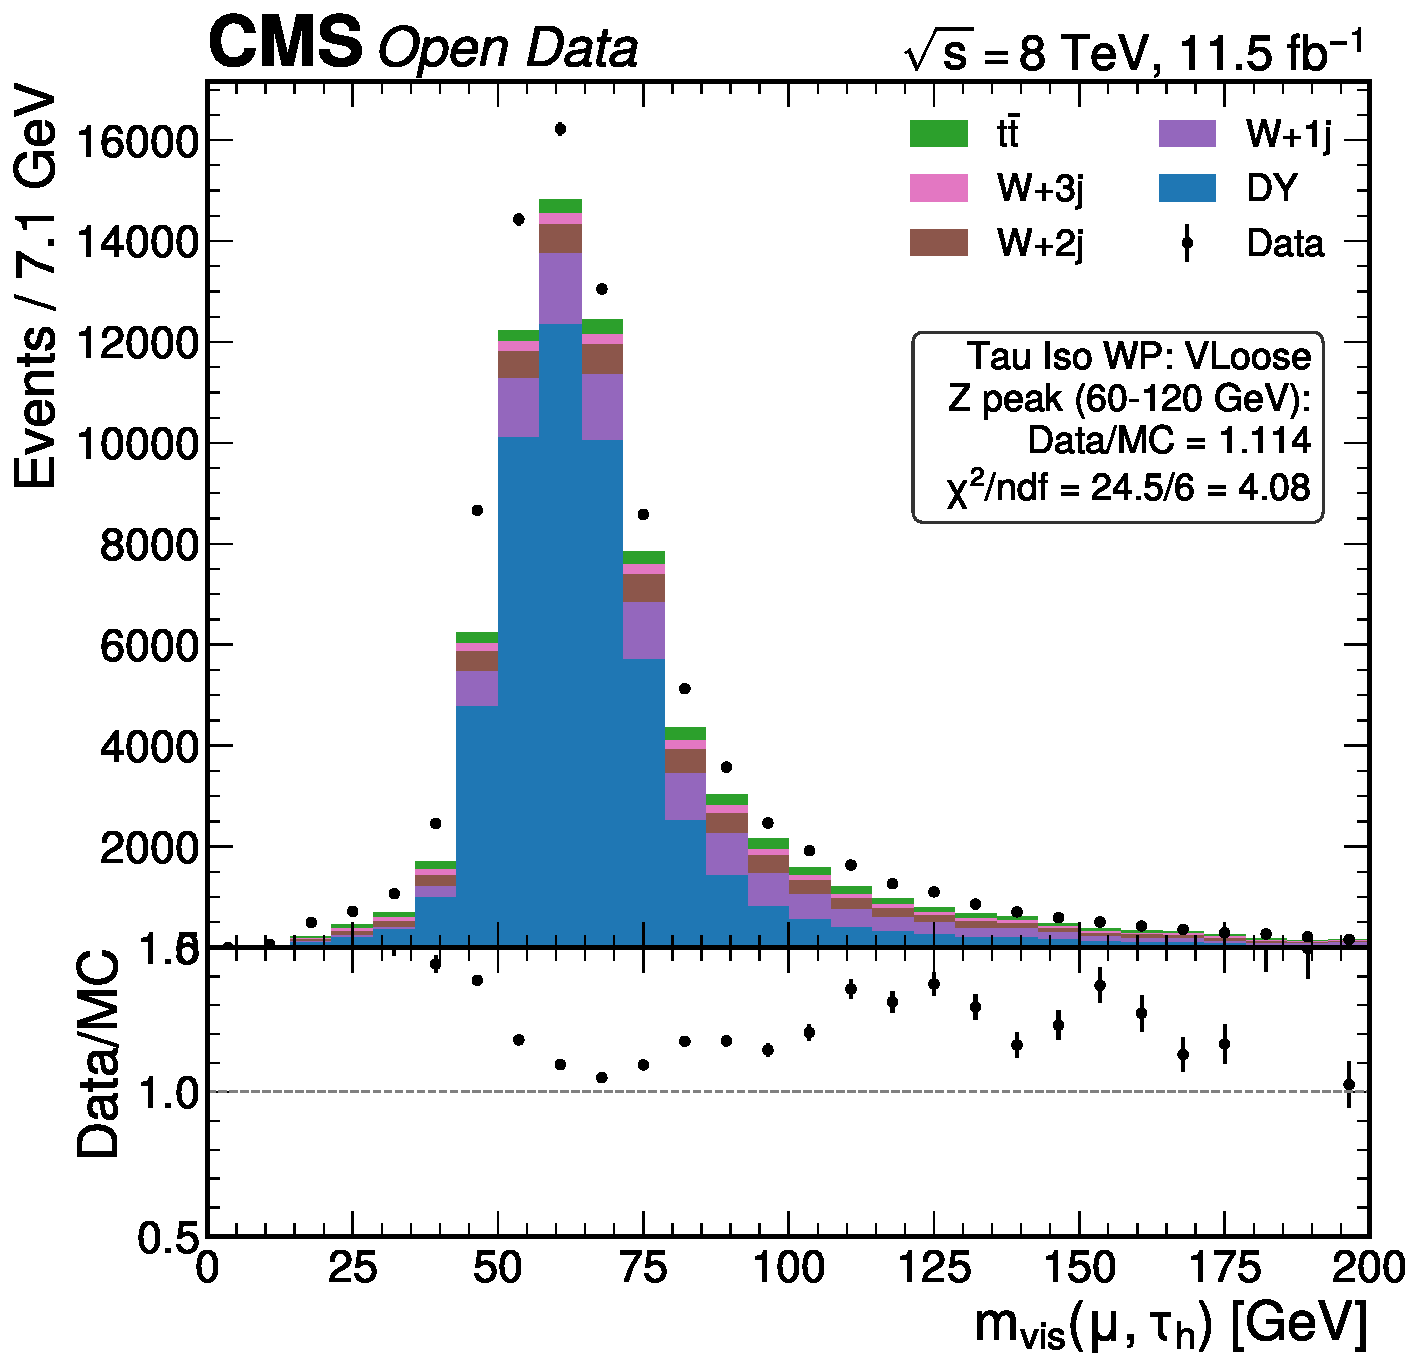
\includegraphics[height=0.28\linewidth,keepaspectratio]{figures/tau_id_wp_VLoose.pdf}\hspace{0.01\linewidth}
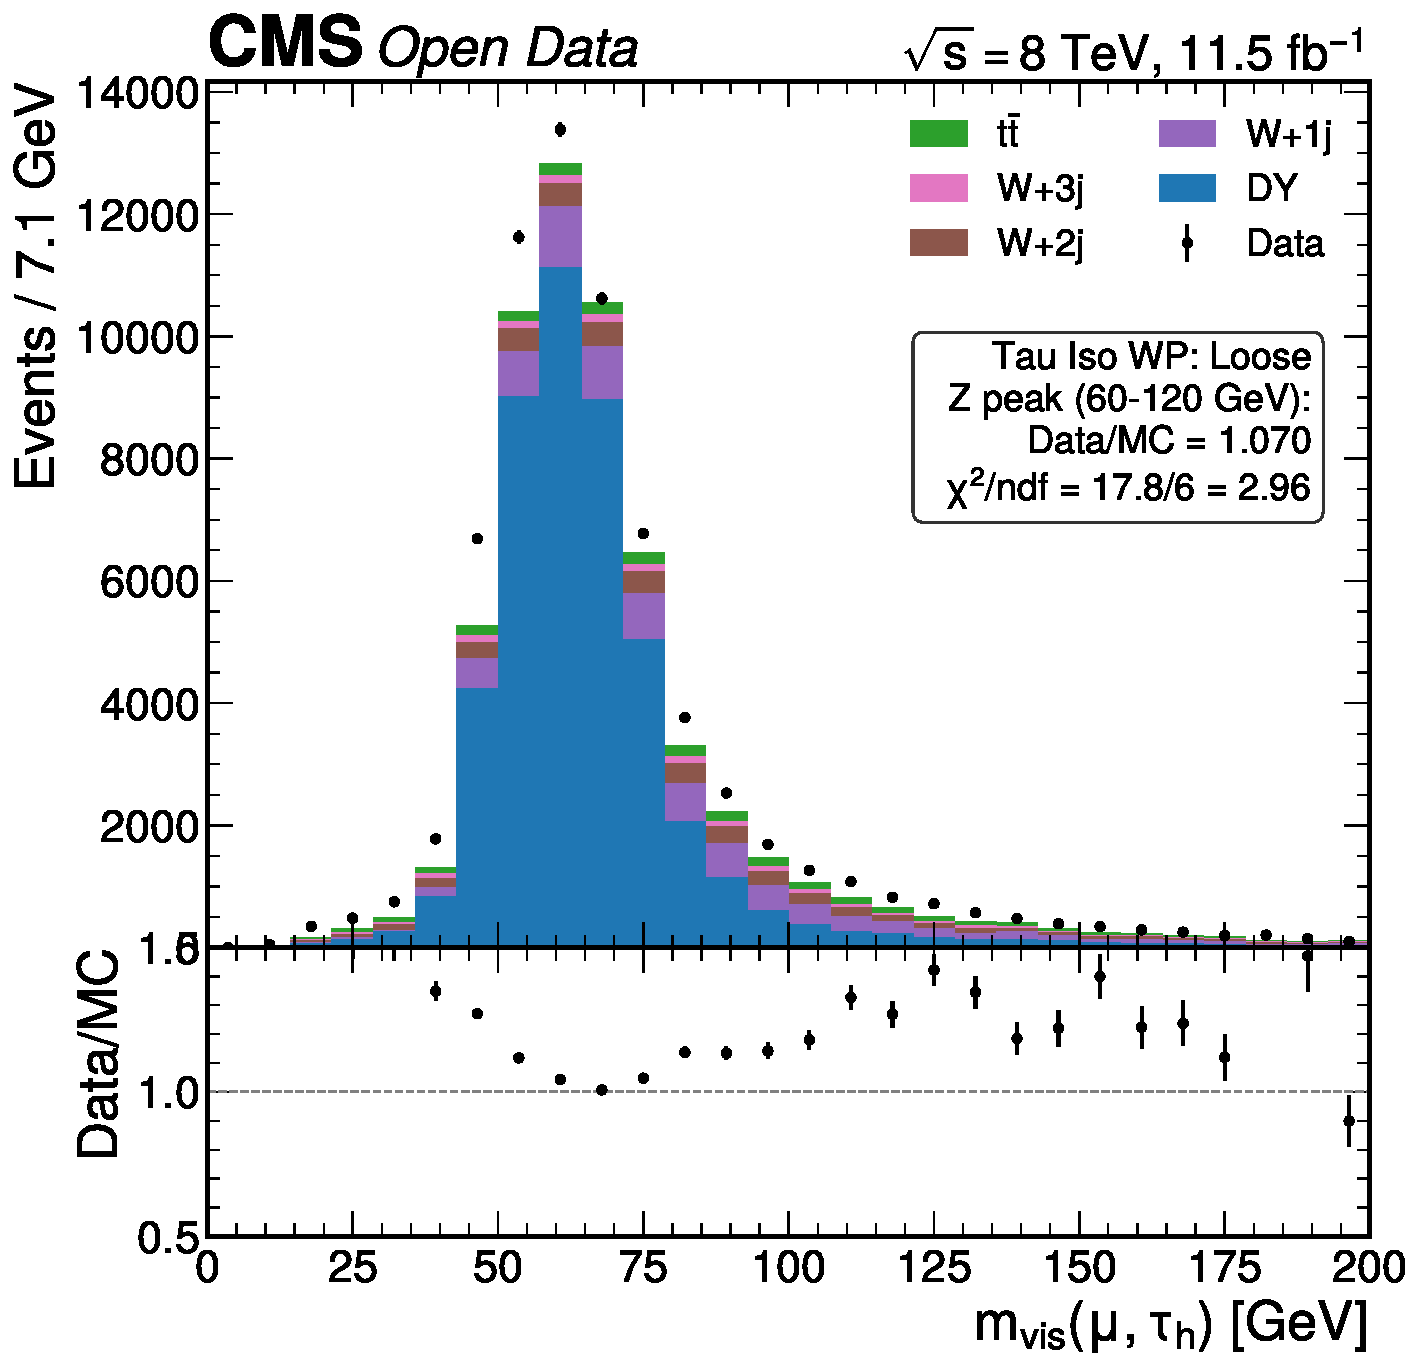
\includegraphics[height=0.28\linewidth,keepaspectratio]{figures/tau_id_wp_Loose.pdf}\hspace{0.01\linewidth}
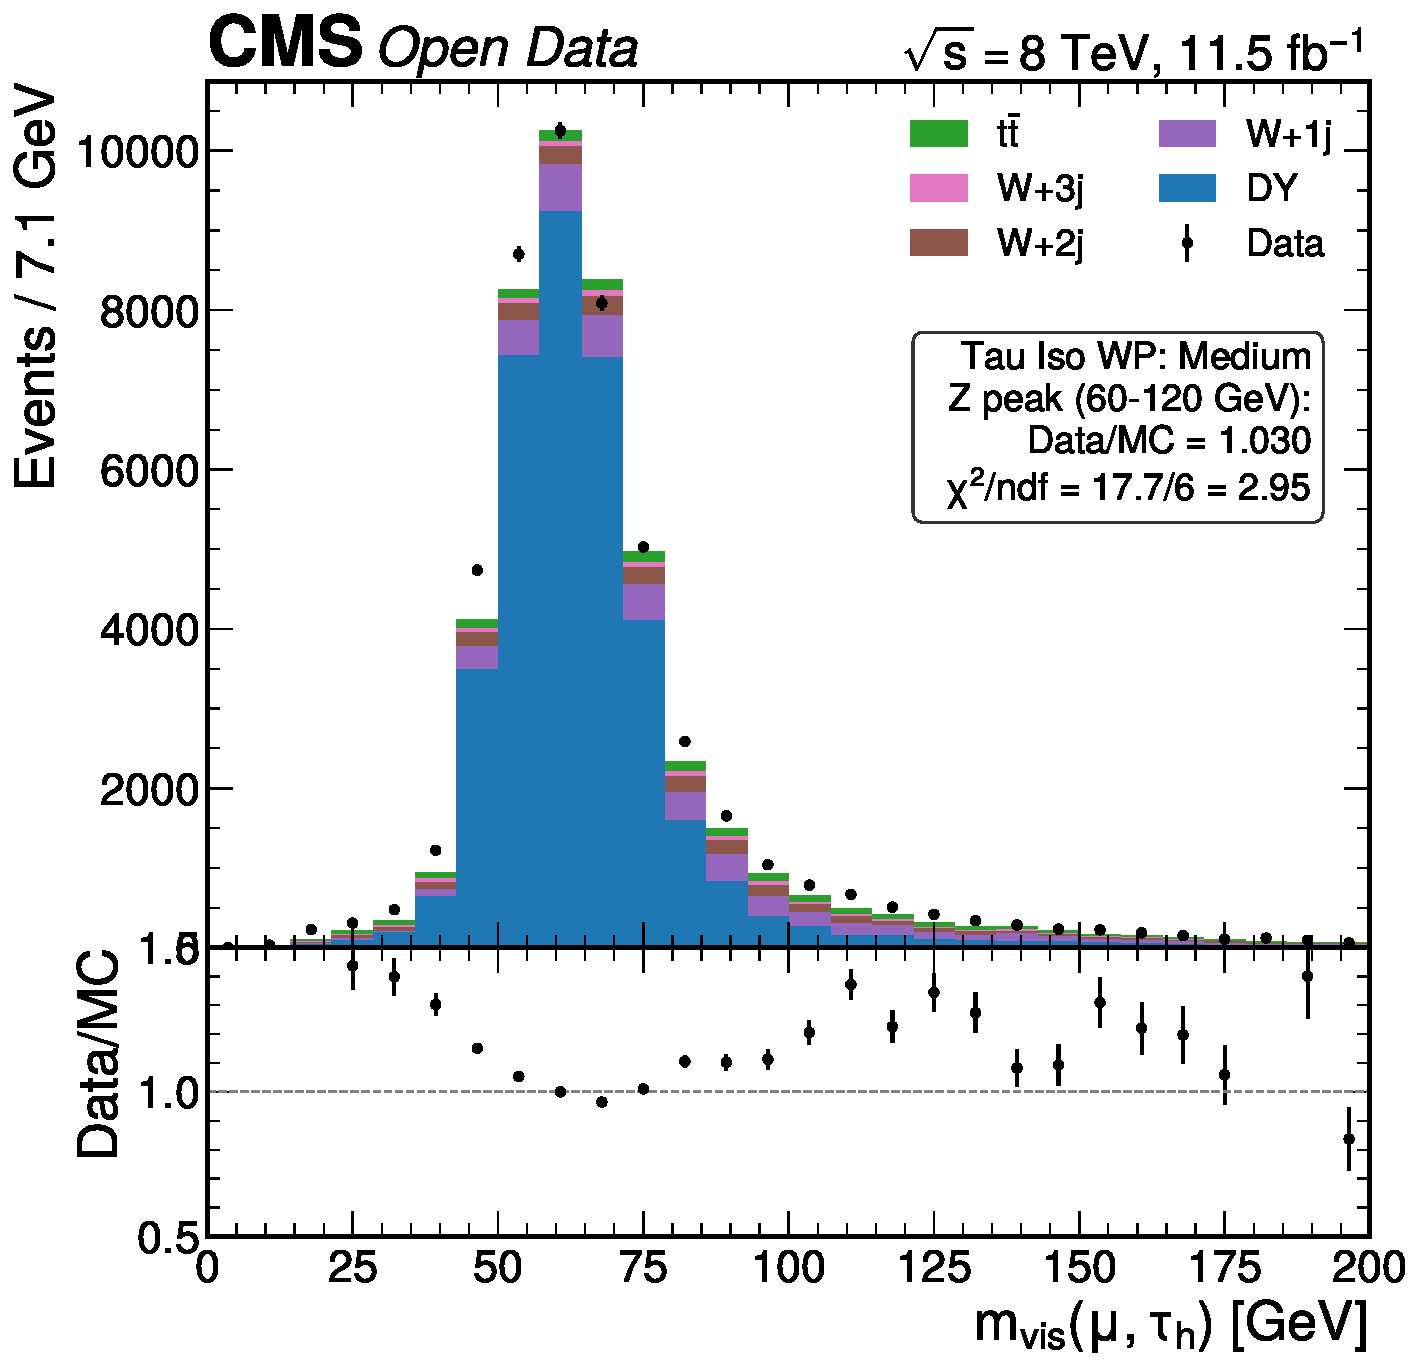
\includegraphics[height=0.28\linewidth,keepaspectratio]{figures/tau_id_wp_Medium.pdf}
\caption{(a) Visible mass distribution with the VLoose tau isolation working
point. The data points show the observed collision data, and the stacked
histogram shows the MC prediction for Z+jets (DY), \(t\bar{t}\), and
W+jets backgrounds. The excess of data over MC in the Z peak region
(\(\chi^2\)/ndf = 4.08) indicates poor modeling at this working point,
motivating the choice of a tighter isolation
requirement. (b) Visible mass distribution with the Loose tau isolation working
point. The data/MC agreement is substantially improved relative to
VLoose (\(\chi^2\)/ndf = 2.96 in the Z peak region), while retaining
20\% more signal yield than the Medium working point. The residual data
excess is attributed to the missing QCD multijet
contribution. (c) Visible mass distribution with the Medium tau isolation working
point. The \(\chi^2\)/ndf of 2.95 is comparable to the Loose working
point, but the signal yield is reduced by 20\%. The slightly lower
Data/MC ratio (1.06 vs 1.12) suggests that the QCD multijet
contamination is smaller at tighter isolation, as
expected.}\label{fig:tauid-vloose}
\phantomsection\label{fig:tauid-loose}
\phantomsection\label{fig:tauid-medium}
\end{figure}


\needspace{4\baselineskip}
\subsection{Control region definitions}\label{sec:control-regions}

Several control regions are defined for background estimation and
validation, as summarized in Table~\ref{tbl:control-regions}.

\vspace{1em}
\begin{table}[htbp]
\centering
\small
\caption{Definition of control regions used for background estimation
and validation. OS and SS denote opposite-sign and same-sign muon-tau
charge requirements,
respectively.}\label{tbl:control-regions}
\begin{tabular}{@{}
lllll@{}}
\toprule\noalign{}
Region & Charge & \(m_\mathrm{T}\) {[}GeV{]} & Muon isolation &
Purpose \\
\midrule\noalign{}
\bottomrule\noalign{}
OS SR & OS & \textless{} 30 & \textless{} 0.1 & Signal region \\
OS high-\(m_\mathrm{T}\) & OS & \textgreater{} 70 & \textless{} 0.1 &
\(W\)+jets normalization \\
OS mid-\(m_\mathrm{T}\) & OS & 30-70 & \textless{} 0.1 & \(W\)+jets
validation \\
SS SR & SS & \textless{} 30 & \textless{} 0.1 & QCD template \\
OS anti-iso & OS & \textless{} 30 & 0.1-0.3 & QCD OS/SS measurement \\
SS anti-iso & SS & \textless{} 30 & 0.1-0.3 & QCD OS/SS measurement \\
\end{tabular}
\end{table}

The high-\(m_\mathrm{T}\) region (\(m_\mathrm{T} > 70\) GeV) is enriched
in \(W\)+jets events (Figure~\ref{fig:mt-regions}) and is used to
derive the \(W\)+jets normalization scale factor (Section~\ref{sec:bkg-wjets}). The same-sign signal region provides the QCD
multijet template after subtraction of MC-predicted same-sign
backgrounds (Section~\ref{sec:bkg-qcd}). The anti-isolated control
regions (0.1 \textless{} muon isolation \textless{} 0.3) are used to
measure the QCD OS/SS charge asymmetry ratio in a QCD-enriched
environment.

\needspace{4\baselineskip}
\subsection{Cutflow}\label{sec:cutflow}

The cutflow for the signal region selection is presented in
Table~\ref{tbl:cutflow-raw} for raw event counts and
Table~\ref{tbl:cutflow-weighted} for luminosity-weighted yields. The
selection proceeds through seven sequential requirements, each designed
to enhance the signal-to-background ratio.

\vspace{1em}
\begin{table}[htbp]
\centering
\small
\caption{Cutflow in raw event counts for each sample. The
\(\Delta R > 0.5\) requirement removes zero events, confirming that the
pair selection criteria naturally produce well-separated
\(\mu\tau_\mathrm{h}\) pairs.}\label{tbl:cutflow-raw}
\resizebox{\textwidth}{!}{%
\begin{tabular}{@{}
>{\raggedright\arraybackslash}p{(\linewidth - 18\tabcolsep) * \real{0.0806}}
  >{\raggedright\arraybackslash}p{(\linewidth - 18\tabcolsep) * \real{0.0806}}
  >{\raggedright\arraybackslash}p{(\linewidth - 18\tabcolsep) * \real{0.0806}}
  >{\raggedright\arraybackslash}p{(\linewidth - 18\tabcolsep) * \real{0.0645}}
  >{\raggedright\arraybackslash}p{(\linewidth - 18\tabcolsep) * \real{0.1935}}
  >{\raggedright\arraybackslash}p{(\linewidth - 18\tabcolsep) * \real{0.0806}}
  >{\raggedright\arraybackslash}p{(\linewidth - 18\tabcolsep) * \real{0.0806}}
  >{\raggedright\arraybackslash}p{(\linewidth - 18\tabcolsep) * \real{0.0806}}
  >{\raggedright\arraybackslash}p{(\linewidth - 18\tabcolsep) * \real{0.1290}}
  >{\raggedright\arraybackslash}p{(\linewidth - 18\tabcolsep) * \real{0.1290}}@{}}
\toprule\noalign{}
\begin{minipage}[b]{\linewidth}\raggedright
Cut
\end{minipage} & \begin{minipage}[b]{\linewidth}\raggedright
ggH
\end{minipage} & \begin{minipage}[b]{\linewidth}\raggedright
VBF
\end{minipage} & \begin{minipage}[b]{\linewidth}\raggedright
DY
\end{minipage} & \begin{minipage}[b]{\linewidth}\raggedright
\(t\bar{t}\)
\end{minipage} & \begin{minipage}[b]{\linewidth}\raggedright
W1J
\end{minipage} & \begin{minipage}[b]{\linewidth}\raggedright
W2J
\end{minipage} & \begin{minipage}[b]{\linewidth}\raggedright
W3J
\end{minipage} & \begin{minipage}[b]{\linewidth}\raggedright
Data B
\end{minipage} & \begin{minipage}[b]{\linewidth}\raggedright
Data C
\end{minipage} \\
\midrule\noalign{}
\toprule\noalign{}
\begin{minipage}[b]{\linewidth}\raggedright
Cut
\end{minipage} & \begin{minipage}[b]{\linewidth}\raggedright
ggH
\end{minipage} & \begin{minipage}[b]{\linewidth}\raggedright
VBF
\end{minipage} & \begin{minipage}[b]{\linewidth}\raggedright
DY
\end{minipage} & \begin{minipage}[b]{\linewidth}\raggedright
\(t\bar{t}\)
\end{minipage} & \begin{minipage}[b]{\linewidth}\raggedright
W1J
\end{minipage} & \begin{minipage}[b]{\linewidth}\raggedright
W2J
\end{minipage} & \begin{minipage}[b]{\linewidth}\raggedright
W3J
\end{minipage} & \begin{minipage}[b]{\linewidth}\raggedright
Data B
\end{minipage} & \begin{minipage}[b]{\linewidth}\raggedright
Data C
\end{minipage} \\
\midrule\noalign{}
\bottomrule\noalign{}
Total & 476,963 & 491,653 & 30,458,871 & 6,423,106 & 29,784,800 &
30,693,853 & 15,241,144 & 35,647,508 & 51,303,171 \\
Trigger & 33,520 & 49,109 & 4,753,620 & 872,546 & 1,251,689 & 2,358,002
& 1,516,331 & 10,038,076 & 13,901,050 \\
Good muon & 25,522 & 39,150 & 4,479,322 & 746,718 & 1,044,071 &
1,969,422 & 1,260,827 & 5,303,043 & 7,917,579 \\
Good \(\tau_\mathrm{h}\) & 8,230 & 10,964 & 77,699 & 53,489 & 41,505 &
73,686 & 42,740 & 142,072 & 224,078 \\
OS pair & 8,069 & 10,556 & 63,279 & 40,556 & 31,314 & 53,476 & 29,928 &
99,109 & 156,267 \\
\(\Delta R > 0.5\) & 8,069 & 10,556 & 63,279 & 40,556 & 31,314 & 53,476
& 29,928 & 99,109 & 156,267 \\
\(m_\mathrm{T} < 30\) & 5,397 & 7,067 & 39,795 & 6,210 & 3,383 & 5,920 &
3,765 & 31,961 & 51,020 \\
Iso \textless{} 0.1 & 4,603 & 6,255 & 34,468 & 5,670 & 2,951 & 5,194 &
3,319 & 26,236 & 41,752 \\
\end{tabular}}%
\end{table}

\vspace{1em}
\begin{table}[htbp]
\centering
\small
\caption{Weighted yields in the opposite-sign signal region after all
selection requirements. The Data/MC ratio of 1.116 is consistent with
the missing QCD multijet
contribution.}\label{tbl:cutflow-weighted}
\begin{tabular}{@{}
lll@{}}
\toprule\noalign{}
Sample & Raw events & Weighted yield \\
\midrule\noalign{}
\bottomrule\noalign{}
ggH (signal) & 4,603 & 148.1 \\
VBF (signal) & 6,255 & 14.6 \\
DY (\(Z\to\tau\tau\)) & 29,747 & 39,237.9 \\
DY (\(Z\to\ell\ell\)) & 4,721 & 6,227.3 \\
\(t\bar{t}\) & 5,670 & 2,560.0 \\
W+1 jet & 2,951 & 7,249.8 \\
W+2 jets & 5,194 & 3,958.1 \\
W+3 jets & 3,319 & 1,529.5 \\
\textbf{MC total} & & \textbf{60,925.3} \\
Data (Run2012B) & 26,236 & 26,236.0 \\
Data (Run2012C) & 41,752 & 41,752.0 \\
\textbf{Data total} & \textbf{67,988} & \textbf{67,988.0} \\
\end{tabular}
\end{table}

The trigger requirement retains approximately 7\% of ggH signal events
and 10\% of VBF signal events. The largest background reduction comes
from the tau identification and isolation requirements, which reject the
vast majority of non-tau jets. The transverse mass requirement
(\(m_\mathrm{T} < 30\) GeV) effectively suppresses the \(W\)+jets
background by a factor of approximately 9 for W+1 jet, while retaining
66\% of the ggH signal. The overall signal selection efficiency (after
trigger) is 13.7\% for ggH and 12.7\% for VBF.

The Data/MC ratio after full selection is 1.116, corresponding to a data
excess of approximately 7,063 events. This excess is attributed to the
missing QCD multijet background, which is estimated from data to
contribute approximately 11,200 events to the signal region (Section~\ref{sec:bkg-qcd}).

\needspace{4\baselineskip}
\subsection{Event categorization}\label{sec:categorization}

Events passing the signal region selection are classified into two
mutually exclusive categories designed to exploit the distinct kinematic
signatures of the VBF and ggH production modes.

\subsubsection{VBF category}\label{vbf-category}

Events are assigned to the VBF category if they contain at least two
jets satisfying:

\begin{equation}\protect\phantomsection\label{eq:vbf-selection}{m_{jj} > 200~\mathrm{GeV} \quad \text{and} \quad |\Delta\eta_{jj}| > 2.0}\end{equation}

These thresholds were optimized in the exploration study using a scan
over the (\(m_{jj}\), \(|\Delta\eta_{jj}|\)) plane to maximize
\(S/\sqrt{B}\) in the VBF category. The optimized thresholds of 200 GeV
and 2.0 are looser than the published CMS analysis values (300 GeV and
2.5) to retain sufficient signal statistics in this single-channel
analysis. The resulting \(S/\sqrt{B}\) in the VBF category is
approximately 0.49.

\subsubsection{Baseline category}\label{baseline-category}

All events passing the signal region selection that do not satisfy the
VBF category criteria are assigned to the Baseline category. This
category is dominated by the ggH production mode and has a larger event
count but lower signal-to-background ratio.

\subsubsection{Category yields}\label{category-yields}

The event yields per category are summarized in
Table~\ref{tbl:category-yields}. The VBF category achieves a VBF signal
purity of 56\% (VBF/(ggH+VBF) = 6.4/11.5), demonstrating effective VBF
enrichment despite modest statistics.

\vspace{1em}
\begin{table}[htbp]
\centering
\small
\caption{Event yields per category in the opposite-sign signal region
(weighted). QCD is estimated separately from
data.}\label{tbl:category-yields}
\begin{tabular}{@{}
lll@{}}
\toprule\noalign{}
Sample & Baseline & VBF \\
\midrule\noalign{}
\bottomrule\noalign{}
ggH & 143.0 & 5.1 \\
VBF & 8.2 & 6.4 \\
DY (\(Z\to\tau\tau + Z\to\ell\ell\)) & 45,052.3 & 412.9 \\
\(t\bar{t}\) & 2,131.1 & 428.9 \\
W+jets & 12,377.7 & 359.7 \\
Data (B+C) & 67,124 & 864 \\
\end{tabular}
\end{table}

\needspace{0.4\textheight}
\begin{figure}[htbp]
\centering
\pandocbounded{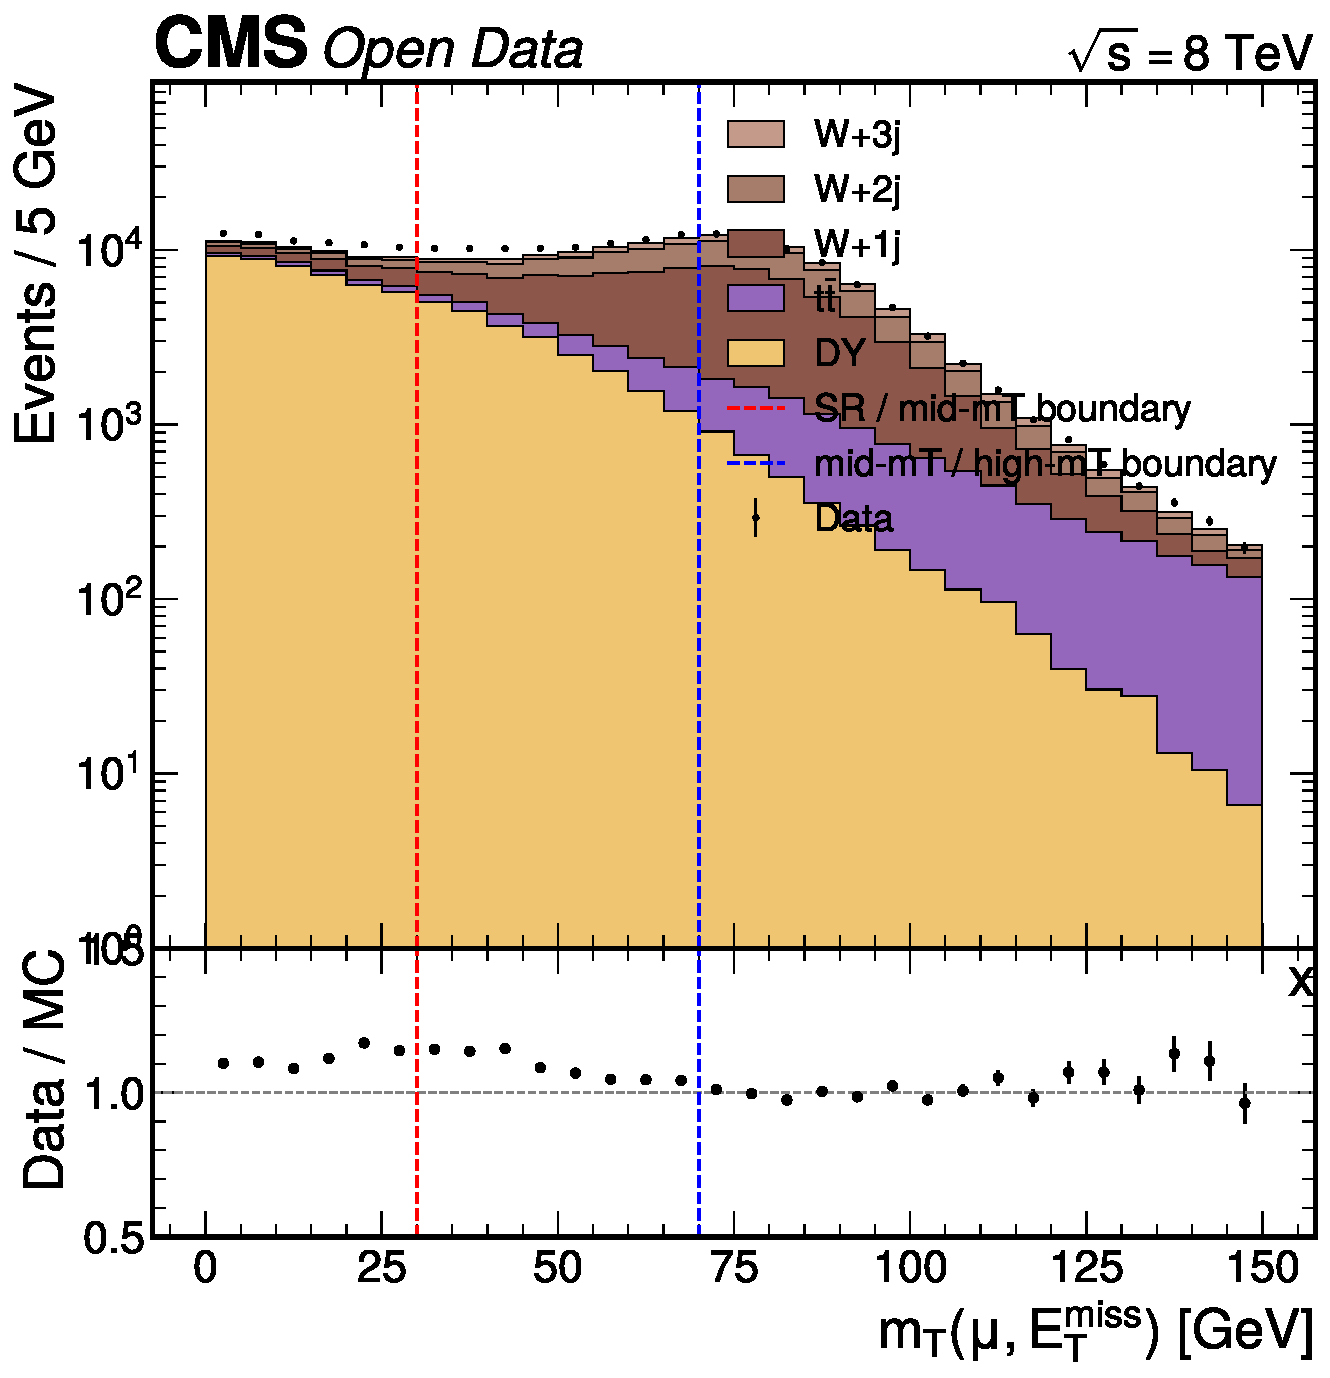
\includegraphics[height=0.35\textheight,width=\linewidth,keepaspectratio,alt={Transverse mass distribution showing the signal region (m\_\textbackslash mathrm\{T\} \textless{} 30 GeV), intermediate validation region (30 \textless{} m\_\textbackslash mathrm\{T\} \textless{} 70 GeV), and high-m\_\textbackslash mathrm\{T\} sideband (m\_\textbackslash mathrm\{T\} \textgreater{} 70 GeV) boundaries. The W+jets background dominates at high m\_\textbackslash mathrm\{T\}, validating its use as the W+jets normalization control region. The signal peaks at low m\_\textbackslash mathrm\{T\} as expected for H\textbackslash to\textbackslash tau\textbackslash tau decays where the muon is nearly balanced by the hadronic tau.}]{figures/mt_regions.pdf}}
\caption{Transverse mass distribution showing the signal region
(\(m_\mathrm{T} < 30\) GeV), intermediate validation region
(\(30 < m_\mathrm{T} < 70\) GeV), and high-\(m_\mathrm{T}\) sideband
(\(m_\mathrm{T} > 70\) GeV) boundaries. The W+jets background dominates
at high \(m_\mathrm{T}\), validating its use as the W+jets normalization
control region. The signal peaks at low \(m_\mathrm{T}\) as expected for
\(H\to\tau\tau\) decays where the muon is nearly balanced by the
hadronic tau.}\label{fig:mt-regions}
\end{figure}

\needspace{4\baselineskip}
\FloatBarrier
\section{Background Estimation}\label{sec:backgrounds}

The backgrounds in the \(\mu\tau_\mathrm{h}\) channel are classified as
irreducible (\(Z\to\tau\tau\)), reducible (\(W\)+jets, \(t\bar{t}\),
\(Z\to\ell\ell\)), or instrumental (QCD multijet). The irreducible
\(Z\to\tau\tau\) background is estimated from MC simulation with a
data-driven normalization uncertainty. The reducible \(W\)+jets
background is normalized using the high-\(m_\mathrm{T}\) data sideband.
The QCD multijet background is estimated entirely from data using the
same-sign control region. The \(t\bar{t}\) and \(Z\to\ell\ell\)
backgrounds are estimated from MC simulation.

\needspace{4\baselineskip}
\subsection{Drell-Yan decomposition}\label{sec:bkg-dy}

The DYJetsToLL MC sample is decomposed into \(Z\to\tau\tau\) (ZTT) and
\(Z\to\ell\ell\) (ZLL) components using generator-level truth matching.
Reconstructed hadronic tau candidates are matched to generator-level tau
leptons (\(|\mathrm{pdgId}| = 15\)) within \(\Delta R < 0.3\). Events
with a truth-matched tau are classified as ZTT; all others are
classified as ZLL.

This decomposition yields 29,747 raw ZTT events (86.3\% of DY, 39,237.9
weighted) and 4,721 raw ZLL events (13.7\% of DY, 6,227.3 weighted) in
the signal region. The ZTT component is the dominant irreducible
background, producing a genuine \(\tau_\mathrm{h}\) in the final state.
The ZLL component arises primarily from \(Z\to\mu\mu\) events where one
muon is misidentified as a hadronic tau. Both components share a common
normalization uncertainty (Section~\ref{sec:syst-znorm}).

\needspace{4\baselineskip}
\subsection{W+jets normalization}\label{sec:bkg-wjets}

The \(W\)+jets background normalization is derived from data in the
high-\(m_\mathrm{T}\) sideband (\(m_\mathrm{T} > 70\) GeV), where
\(W\)+jets events dominate. The scale factor is defined as:

\begin{equation}\protect\phantomsection\label{eq:wjets-sf}{\mathrm{SF}_W = \frac{N_\mathrm{data}^\mathrm{high\text{-}mT} - N_\mathrm{non\text{-}W~MC}^\mathrm{high\text{-}mT}}{N_{W\mathrm{+jets~MC}}^\mathrm{high\text{-}mT}}}\end{equation}

The measured quantities and resulting scale factor are:

\vspace{1em}
\begin{table}[htbp]
\centering
\small
\caption{W+jets normalization scale factor derived from the
high-\(m_\mathrm{T}\) sideband. The uncertainty includes weighted MC
statistical propagation
(\(\sigma^2_\mathrm{MC} = \sum w_i^2\)).}\label{tbl:wjets-sf}
\begin{tabular}{@{}
ll@{}}
\toprule\noalign{}
Quantity & Value \\
\midrule\noalign{}
\bottomrule\noalign{}
Data (\(m_\mathrm{T} > 70\) GeV) & 65,765 \\
Non-\(W\) MC (\(m_\mathrm{T} > 70\) GeV) & 12,013.5 \\
\(W\)+jets MC (\(m_\mathrm{T} > 70\) GeV) & 53,801.0 \\
\textbf{\(\mathrm{SF}_W\)} & \textbf{0.999 ± 0.008} \\
\end{tabular}
\end{table}

The scale factor is consistent with unity, indicating that the W+jets MC
normalization using the MadGraph LO cross-sections is accurate. The
small statistical uncertainty of 0.8\% is subdominant compared to the
10\% systematic uncertainty assigned to the \(W\)+jets normalization to
account for the \(m_\mathrm{T}\) extrapolation from the sideband to the
signal region (Section~\ref{sec:syst-wjets}).

\subsubsection{\texorpdfstring{Validation in the
intermediate-\(m_\mathrm{T}\)
region}{Validation in the intermediate-m\_\textbackslash mathrm\{T\} region}}\label{validation-in-the-intermediate-m_mathrmt-region}

The \(W\)+jets normalization is validated in the intermediate transverse
mass region (\(30 < m_\mathrm{T} < 70\) GeV), which is kinematically
between the signal region and the normalization sideband. The predicted
Data/MC ratio in this region is 1.087 after applying \(\mathrm{SF}_W\)
(Figure~\ref{fig:wjets-validation}), with the 8.7\% residual excess
consistent with QCD multijet contamination in this region.

\needspace{0.4\textheight}
\begin{figure}[htbp]
\centering
\pandocbounded{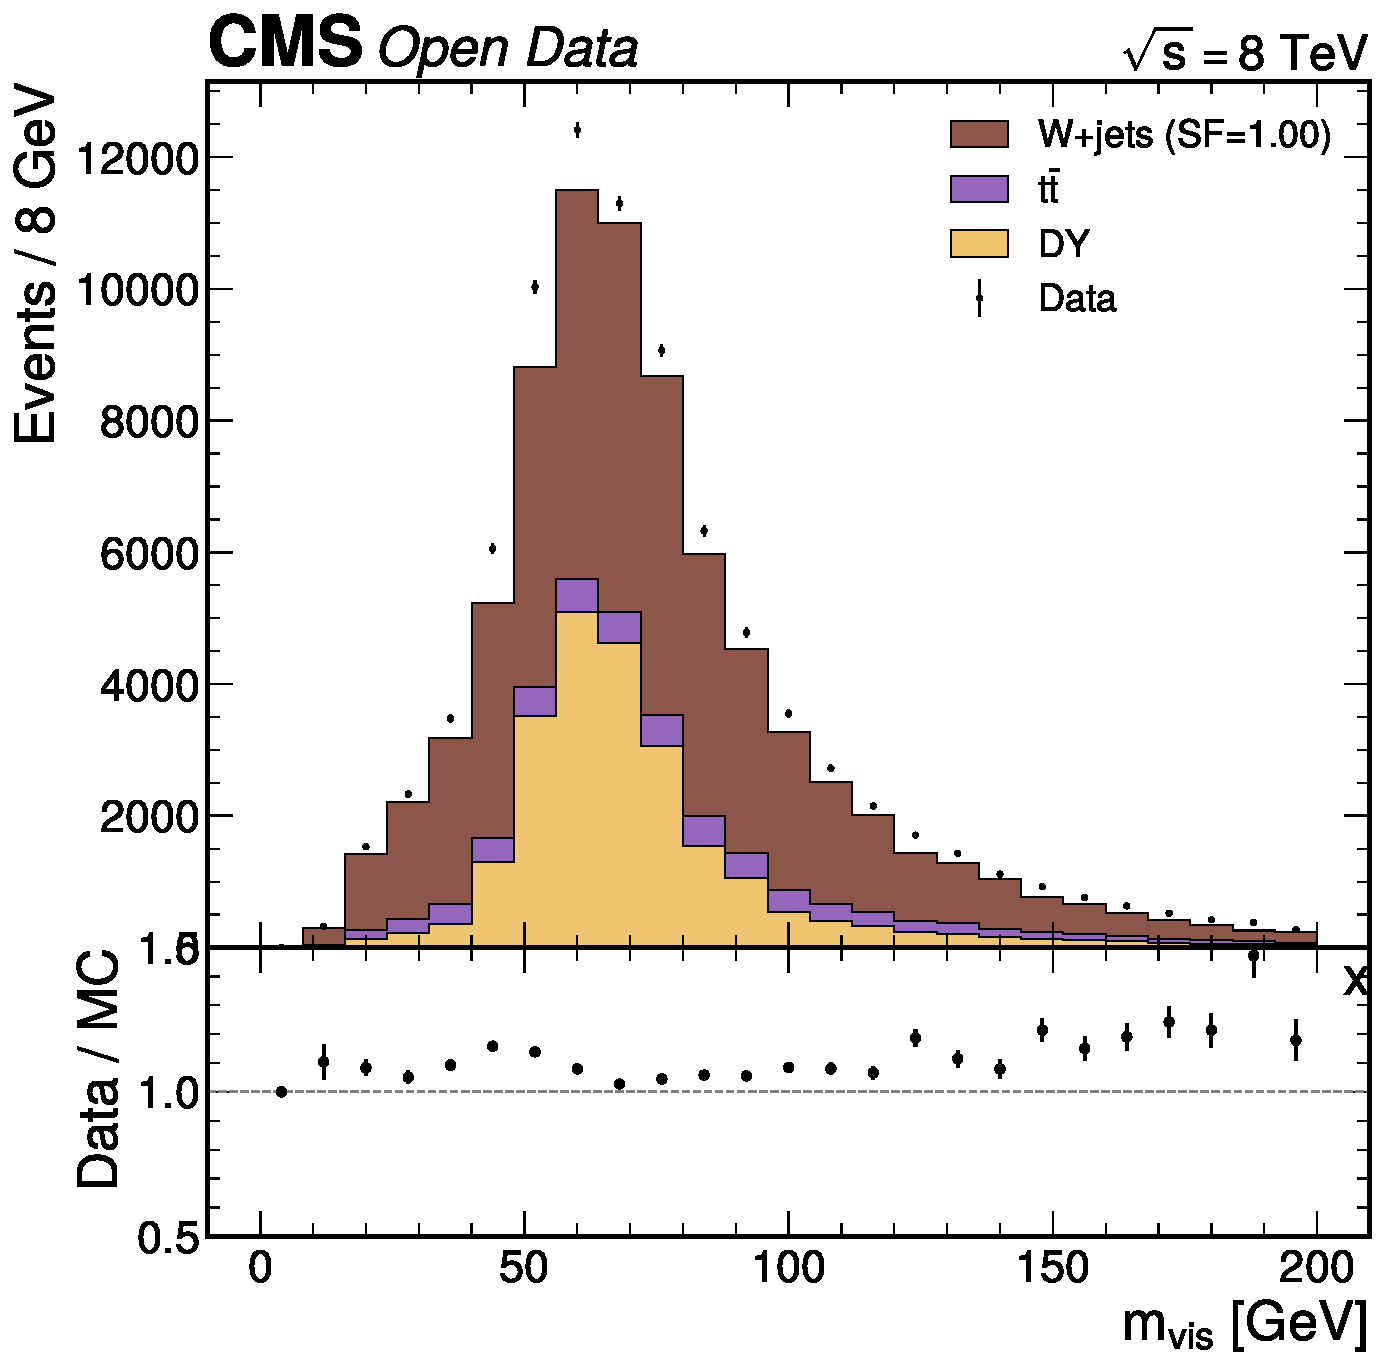
\includegraphics[height=0.35\textheight,width=\linewidth,keepaspectratio,alt={Validation of the W+jets normalization in the intermediate-m\_\textbackslash mathrm\{T\} region (30 \textless{} m\_\textbackslash mathrm\{T\} \textless{} 70 GeV). The data points are compared to the MC prediction with the W+jets scale factor applied. The Data/Pred ratio of 1.087 is consistent with the expected QCD multijet contribution that is not included in this validation.}]{figures/wjets_validation_midmt.pdf}}
\caption{Validation of the W+jets normalization in the
intermediate-\(m_\mathrm{T}\) region (\(30 < m_\mathrm{T} < 70\) GeV).
The data points are compared to the MC prediction with the W+jets scale
factor applied. The Data/Pred ratio of 1.087 is consistent with the
expected QCD multijet contribution that is not included in this
validation.}\label{fig:wjets-validation}
\end{figure}

\needspace{4\baselineskip}
\subsection{QCD multijet estimation}\label{sec:bkg-qcd}

The QCD multijet background is estimated from data using the same-sign
(SS) control region method. QCD multijet events produce
\(\mu\tau_\mathrm{h}\) pairs with approximately equal rates of
opposite-sign and same-sign configurations, with a small charge
asymmetry quantified by the OS/SS ratio \(R_\mathrm{OS/SS}\).

\subsubsection{OS/SS ratio measurement}\label{osss-ratio-measurement}

The OS/SS ratio is measured in a QCD-enriched anti-isolated control
region (\(0.1 < I_\mathrm{rel}^\mathrm{PF}(\mu) < 0.3\)) after
subtracting non-QCD MC backgrounds:

\begin{equation}\protect\phantomsection\label{eq:osss-ratio}{R_\mathrm{OS/SS} = \frac{N_\mathrm{data}^\mathrm{OS,anti\text{-}iso} - N_\mathrm{MC}^\mathrm{OS,anti\text{-}iso}}{N_\mathrm{data}^\mathrm{SS,anti\text{-}iso} - N_\mathrm{MC}^\mathrm{SS,anti\text{-}iso}}}\end{equation}

The measured value is \(R_\mathrm{OS/SS} = 0.979 \pm 0.018\), where the
uncertainty is statistical. This value lies between the CMS Open Data
tutorial value (0.80) and the published analysis value (1.06),
reflecting the specific isolation and kinematic requirements of this
selection. The 30\% spread among these reference values motivated the
data-driven measurement rather than adopting a literature value.

\subsubsection{QCD yield in the signal
region}\label{qcd-yield-in-the-signal-region}

The QCD yield in the opposite-sign signal region is estimated as:

\begin{equation}\protect\phantomsection\label{eq:qcd-yield}{N_\mathrm{QCD}^\mathrm{OS~SR} = R_\mathrm{OS/SS} \times \left( N_\mathrm{data}^\mathrm{SS~SR} - N_\mathrm{MC}^\mathrm{SS~SR} \right)}\end{equation}

\vspace{1em}
\begin{table}[htbp]
\centering
\small
\caption{QCD multijet yield estimation. The uncertainty is statistical,
propagated from the data and MC statistical
uncertainties.}\label{tbl:qcd-yield}
\begin{tabular}{@{}
ll@{}}
\toprule\noalign{}
Quantity & Value \\
\midrule\noalign{}
\bottomrule\noalign{}
Data (SS SR) & 23,134 \\
MC (SS SR) & 11,704.2 \\
QCD (SS) = Data - MC & 11,429.8 \\
\textbf{QCD (OS) estimate} & \textbf{11,195.5 ± 230.6} \\
\end{tabular}
\end{table}

The QCD template shape is taken from the SS data after MC subtraction.
The NN scores and collinear mass values for the QCD template are
computed by evaluating the trained NN model and collinear mass algorithm
on the same-sign events, ensuring that the QCD template shape is
consistent with the fitting observable in each approach.

\needspace{4\baselineskip}
\subsection{Corrected yield summary}\label{sec:bkg-summary}

Table~\ref{tbl:corrected-yields} summarizes the predicted yields from all
background sources and signal in the opposite-sign signal region after
applying all data-driven corrections.

\vspace{1em}
\begin{table}[htbp]
\centering
\small
\caption{Corrected yield summary in the signal region. The 6\% deficit
of data relative to the prediction suggests a slight overestimate of the
QCD contribution, which will be absorbed by the QCD normalization
nuisance parameter in the template
fit.}\label{tbl:corrected-yields}
\begin{tabular}{@{}
ll@{}}
\toprule\noalign{}
Source & OS SR yield \\
\midrule\noalign{}
\bottomrule\noalign{}
DY (\(Z\to\tau\tau\)) & 39,237.9 \\
DY (\(Z\to\ell\ell\)) & 6,227.3 \\
\(t\bar{t}\) & 2,560.0 \\
\(W\)+jets (\(\mathrm{SF} = 0.999\)) & 12,727.5 \\
QCD (data-driven) & 11,195.5 \\
Signal (ggH + VBF) & 162.7 \\
\textbf{Total prediction} & \textbf{72,111.0} \\
\textbf{Data} & \textbf{67,988.0} \\
\textbf{Data/Pred} & \textbf{0.943} \\
\end{tabular}
\end{table}

The total Data/Prediction ratio of 0.943 indicates a 6\% deficit of data
relative to the full prediction, suggesting that the QCD same-sign
estimation slightly overestimates the QCD contribution in the signal
region. This overestimation is within the 20\% systematic uncertainty
assigned to the QCD normalization and will be absorbed by the QCD
normalization nuisance parameter in the template fit.

\needspace{4\baselineskip}
\FloatBarrier
\section{Discriminant Variables}\label{sec:discriminants}

Three fitting approaches are implemented, differing only in the
discriminant variable used in the template fit. All approaches share the
same event selection, categorization, and background estimation.

\needspace{4\baselineskip}
\subsection{Visible di-tau mass}\label{sec:disc-mvis}

The visible di-tau mass is defined as the invariant mass of the muon and
hadronic tau system:

\begin{equation}\protect\phantomsection\label{eq:mvis}{m_\mathrm{vis} = \sqrt{(p_\mu + p_{\tau_\mathrm{h}})^2}}\end{equation}

This is the simplest observable and provides a direct physical
interpretation. The Higgs signal appears as a broad excess in the
100-150 GeV region, sitting on the tail of the \(Z\to\tau\tau\) peak
near 60-80 GeV (in visible mass), as shown in Figures~\ref{fig:mvis-baseline} and Figure~\ref{fig:mvis-vbf}. The poor mass
resolution (approximately 30-40 GeV) arises from the undetected
neutrinos in both tau decays. Templates are constructed in 25
equal-width bins from 0 to 250 GeV (10 GeV/bin).

\needspace{0.4\textheight}
\begin{figure}[htbp]
\centering
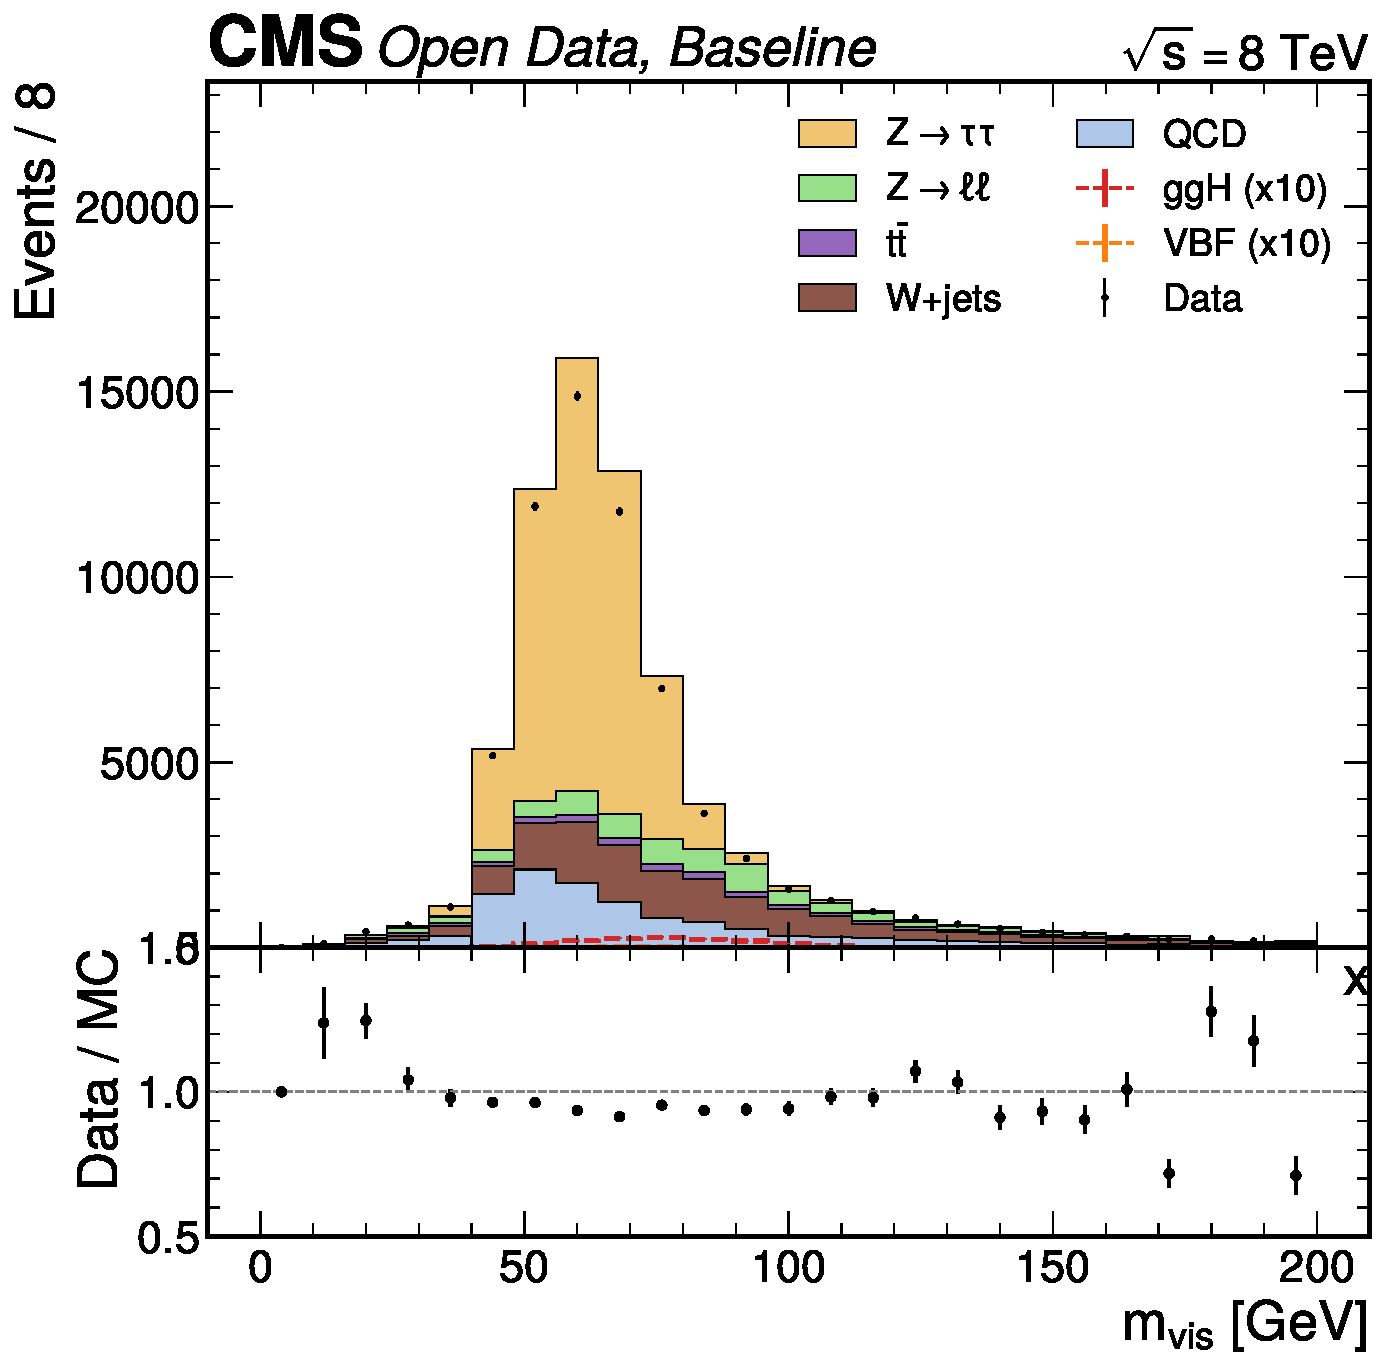
\includegraphics[height=0.38\linewidth,keepaspectratio]{figures/mvis_baseline.pdf}\hspace{0.02\linewidth}
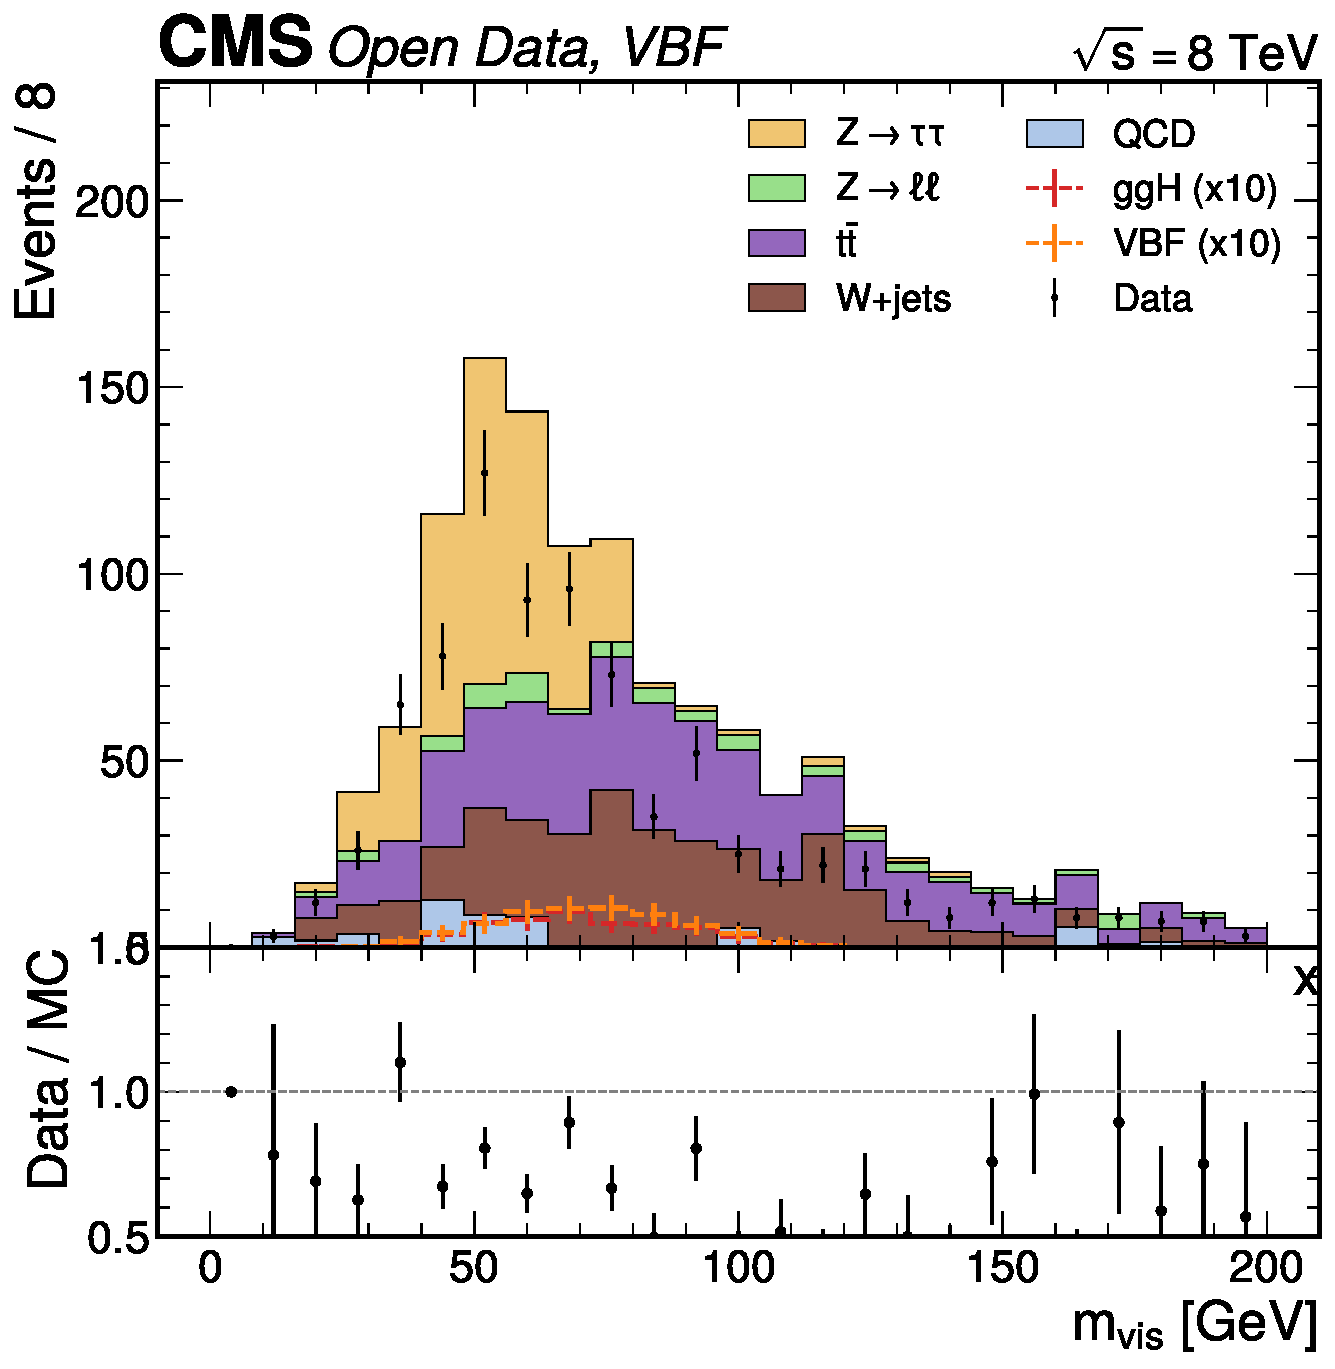
\includegraphics[height=0.38\linewidth,keepaspectratio]{figures/mvis_vbf.pdf}
\caption{(a) Visible mass distribution in the Baseline category. Data points
show the observed collision data, and the stacked histogram shows the MC
prediction with Drell-Yan decomposed into \(Z\to\tau\tau\) (ZTT, blue)
and \(Z\to\ell\ell\) (ZLL, light blue), \(t\bar{t}\) (green), W+jets
(purple), and QCD multijet from the same-sign data estimate (yellow).
The ggH and VBF signal contributions are shown scaled by a factor of 10
for visibility. The \(Z\) peak is clearly visible near 60-80 GeV, with
the expected Higgs signal region at higher
masses. (b) Visible mass distribution in the VBF category (\(m_{jj} > 200\)
GeV, \(|\Delta\eta_{jj}| > 2.0\)). The lower statistics compared to the
Baseline category are evident, with the \(t\bar{t}\) and W+jets
backgrounds becoming more prominent relative to the Drell-Yan
contribution. The data/MC ratio fluctuations are larger due to the
reduced event count.}\label{fig:mvis-baseline}
\phantomsection\label{fig:mvis-vbf}
\end{figure}


\needspace{4\baselineskip}
\subsection{Neural network discriminant}\label{sec:disc-nn}

\subsubsection{Architecture and
training}\label{architecture-and-training}

A neural network classifier is trained to distinguish \(H\to\tau\tau\)
signal from all backgrounds using the scikit-learn MLPClassifier
(\citeproc{ref-Pedregosa:2011skl}{{Pedregosa et al.} 2011}). The
architecture and training configuration are summarized in
Table~\ref{tbl:nn-config}.

\vspace{1em}
\begin{table}[htbp]
\centering
\small
\caption{Neural network classifier configuration. The architecture was
selected to provide sufficient capacity for the 14-dimensional input
space while maintaining regularization to prevent
overtraining.}\label{tbl:nn-config}
\begin{tabular}{@{}
ll@{}}
\toprule\noalign{}
Parameter & Value \\
\midrule\noalign{}
\bottomrule\noalign{}
Framework & scikit-learn MLPClassifier \\
Architecture & 3 hidden layers: 64-64-32 \\
Activation & ReLU \\
Regularization & L2 (\(\alpha = 0.001\)) \\
Optimizer & Adam (lr = 0.001, adaptive) \\
Batch size & 256 \\
Early stopping & Yes (validation fraction = 0.1) \\
Convergence & 30 iterations \\
Random seed & 42 \\
\end{tabular}
\end{table}

\subsubsection{Input features}\label{input-features}

The NN uses 15 input features, listed in Table~\ref{tbl:nn-features} with
their individual signal-vs-background separation power as measured by
the ROC AUC.

\vspace{1em}
\begin{longtable}[]{@{}
  >{\raggedright\arraybackslash}p{(\linewidth - 4\tabcolsep) * \real{0.2903}}
  >{\raggedright\arraybackslash}p{(\linewidth - 4\tabcolsep) * \real{0.4194}}
  >{\raggedright\arraybackslash}p{(\linewidth - 4\tabcolsep) * \real{0.2903}}@{}}
\caption{Neural network input features with their individual
discriminating power (ROC AUC for signal vs background separation).
Features are listed approximately in order of decreasing individual
separation power.}\label{tbl:nn-features}\tabularnewline
\toprule\noalign{}
\begin{minipage}[b]{\linewidth}\raggedright
Feature
\end{minipage} & \begin{minipage}[b]{\linewidth}\raggedright
Description
\end{minipage} & \begin{minipage}[b]{\linewidth}\raggedright
ROC AUC
\end{minipage} \\
\midrule\noalign{}
\endfirsthead
\toprule\noalign{}
\begin{minipage}[b]{\linewidth}\raggedright
Feature
\end{minipage} & \begin{minipage}[b]{\linewidth}\raggedright
Description
\end{minipage} & \begin{minipage}[b]{\linewidth}\raggedright
ROC AUC
\end{minipage} \\
\midrule\noalign{}
\endhead
\bottomrule\noalign{}
\endlastfoot
\(\tau_\mathrm{h}\) \(p_\mathrm{T}\) & Hadronic tau transverse momentum
& 0.695 \\
\(m_\mathrm{vis}\) & Visible di-tau mass & 0.656 \\
\(N_\mathrm{jets}\) & Number of jets & 0.647 \\
\(E_\mathrm{T}^\mathrm{miss}\) & Missing transverse energy & 0.639 \\
\(\Delta R(\mu, \tau_\mathrm{h})\) & Angular separation & 0.564 \\
\(\mu\) \(p_\mathrm{T}\) & Muon transverse momentum & 0.561 \\
\(\tau_\mathrm{h}\) decay mode & Tau decay mode & 0.554 \\
\(m_\mathrm{T}(\mu, E_\mathrm{T}^\mathrm{miss})\) & Transverse mass &
0.554 \\
\(\Delta\phi(\mu, \tau_\mathrm{h})\) & Azimuthal separation & 0.554 \\
\(E_\mathrm{T}^\mathrm{miss}\) significance & MET significance & N/A \\
\(\mu\) \(\eta\) & Muon pseudorapidity & 0.507 \\
\(\tau_\mathrm{h}\) \(\eta\) & Tau pseudorapidity & 0.503 \\
Leading jet \(p_\mathrm{T}\) & Leading jet transverse momentum & N/A \\
Leading jet \(\eta\) & Leading jet pseudorapidity & N/A \\
\(N_\mathrm{b-jets}\) & Number of b-jets & 0.507 \\
\end{longtable}

\subsubsection{Training sample and
performance}\label{training-sample-and-performance}

The training uses the signal region MC events split into 50\% training,
25\% validation, and 25\% test sets with random seed 42. Signal events
(ggH + VBF, 10,858 unweighted) are reweighted to have the same total
weight as background events (51,602 unweighted) for balanced training.

\vspace{1em}
\begin{table}[htbp]
\centering
\small
\caption{NN classifier performance. The test AUC of 0.825 exceeds the
go/no-go threshold of 0.75 established in the analysis
strategy.}\label{tbl:nn-performance}
\begin{tabular}{@{}
llll@{}}
\toprule\noalign{}
Metric & Train & Validation & Test \\
\midrule\noalign{}
\bottomrule\noalign{}
AUC & 0.8426 & 0.8325 & 0.8250 \\
\end{tabular}
\end{table}

The test AUC of 0.825 exceeds the go/no-go threshold of 0.75, confirming
that the NN provides meaningful signal-background discrimination (Figure~\ref{fig:nn-roc}). The modest drop from train (0.843) to test
(0.825) AUC indicates good generalization with no significant
overtraining (Figure~\ref{fig:nn-overtraining}). The NN assigns
mean scores of 0.67-0.79 to signal events and 0.26-0.35 to background
events, with data mean scores (0.32) consistent with the background
expectation.

\subsubsection{Overtraining validation}\label{overtraining-validation}

The absence of overtraining is confirmed by the Kolmogorov-Smirnov (KS)
test between the training and test score distributions:

\vspace{1em}
\begin{table}[htbp]
\centering
\small
\caption{KS test for overtraining between training and test NN score
distributions. Both \(p\)-values exceed 0.05, confirming no significant
overtraining.}\label{tbl:nn-overtraining}
\begin{tabular}{@{}
llll@{}}
\toprule\noalign{}
Class & KS statistic & \(p\)-value & Verdict \\
\midrule\noalign{}
\bottomrule\noalign{}
Signal & 0.0275 & 0.127 & No overtraining \\
Background & 0.0077 & 0.686 & No overtraining \\
\end{tabular}
\end{table}

\needspace{0.4\textheight}
\begin{figure}[htbp]
\centering
\pandocbounded{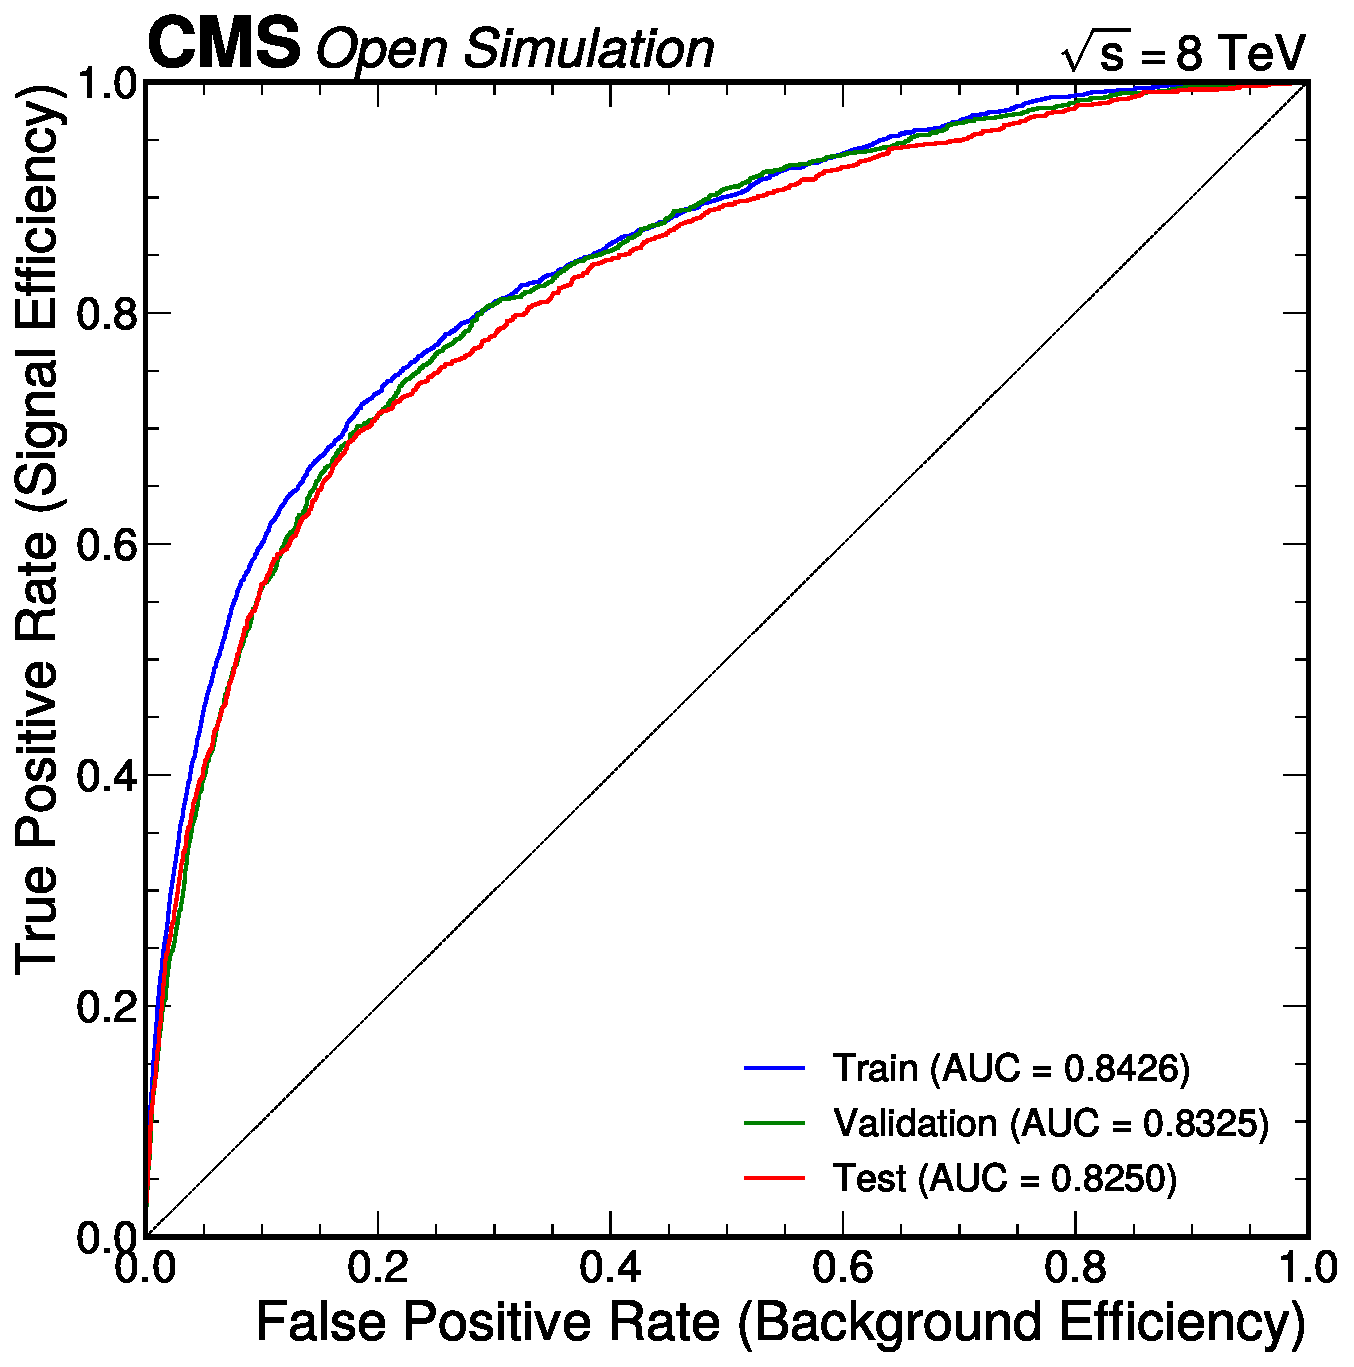
\includegraphics[height=0.35\textheight,width=\linewidth,keepaspectratio,alt={ROC curves for the NN classifier on the training, validation, and test datasets. The three curves are consistent, confirming no overtraining. The test AUC of 0.825 demonstrates significant discriminating power between signal and background.}]{figures/nn_roc.pdf}}
\caption{ROC curves for the NN classifier on the training, validation,
and test datasets. The three curves are consistent, confirming no
overtraining. The test AUC of 0.825 demonstrates significant
discriminating power between signal and background.}\label{fig:nn-roc}
\end{figure}

\needspace{0.4\textheight}
\begin{figure}[htbp]
\centering
\pandocbounded{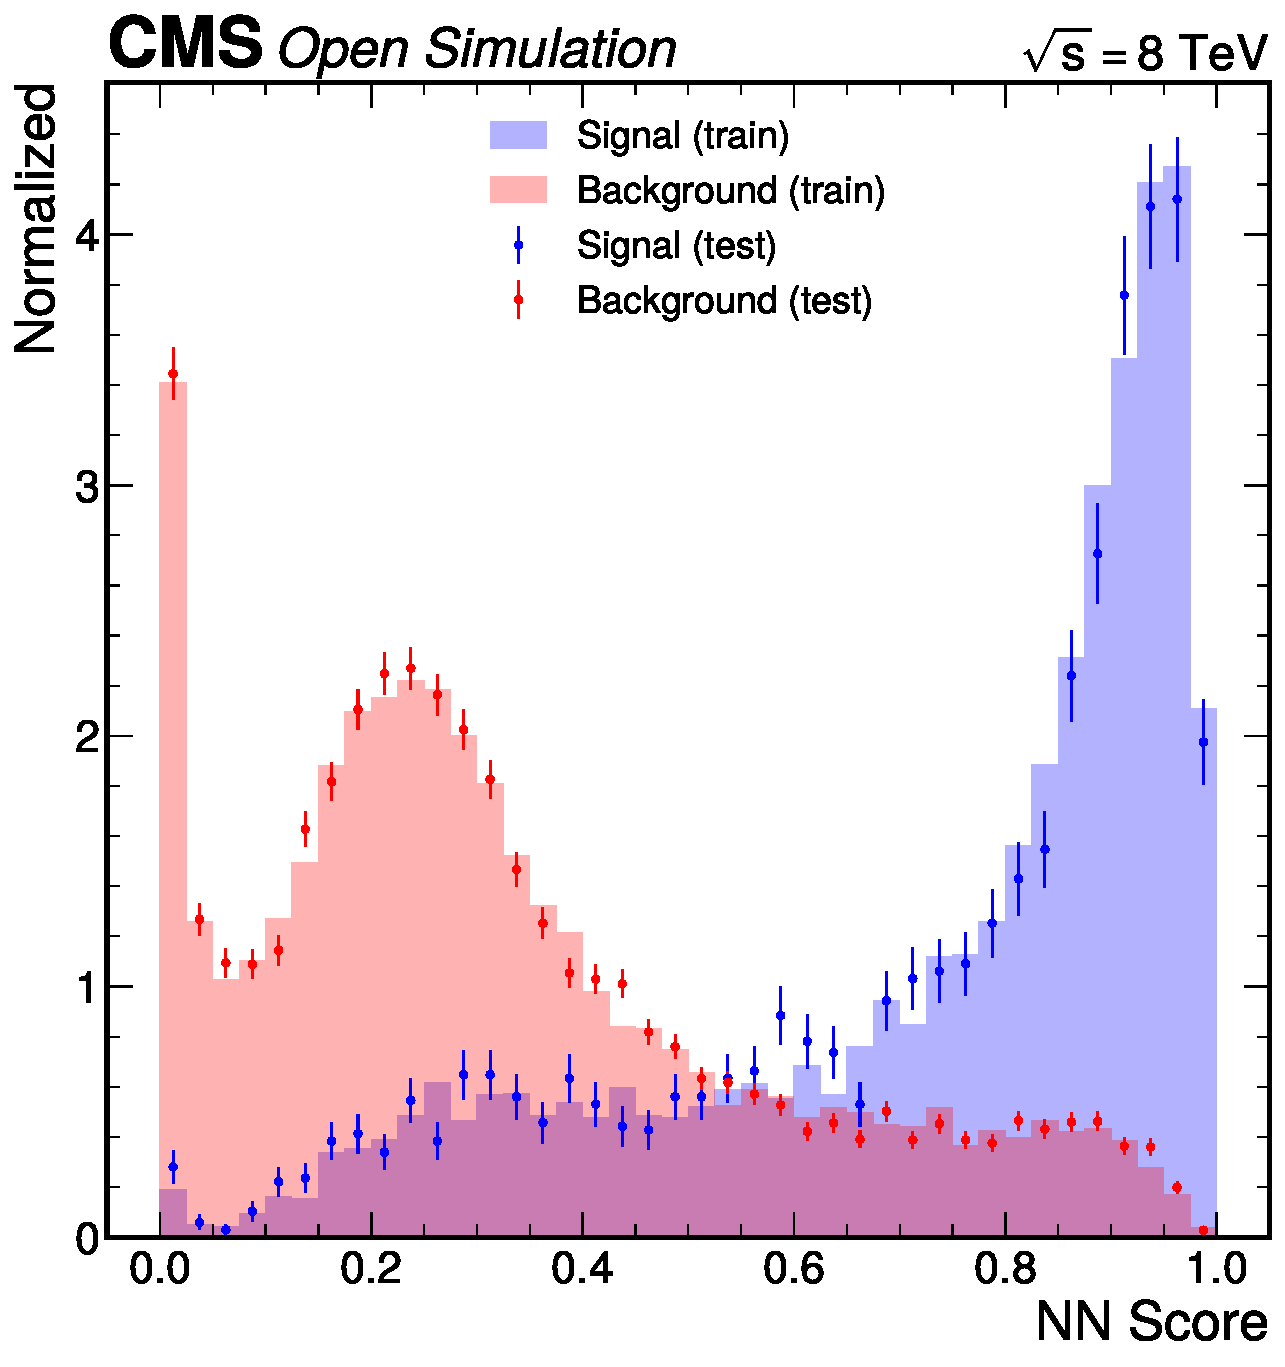
\includegraphics[height=0.35\textheight,width=\linewidth,keepaspectratio,alt={Overtraining check for the NN classifier. The NN score distributions are shown for signal (red) and background (blue), overlaying the training set (filled histogram) and test set (points with error bars). The good agreement between training and test distributions in both classes confirms the absence of overtraining, consistent with the KS test results in tbl.~.}]{figures/nn_overtraining.pdf}}
\caption{Overtraining check for the NN classifier. The NN score
distributions are shown for signal (red) and background (blue),
overlaying the training set (filled histogram) and test set (points with
error bars). The good agreement between training and test distributions
in both classes confirms the absence of overtraining, consistent with
the KS test results in
Table~\ref{tbl:nn-overtraining}.}\label{fig:nn-overtraining}
\end{figure}

\needspace{0.4\textheight}
\begin{figure}[htbp]
\centering
\pandocbounded{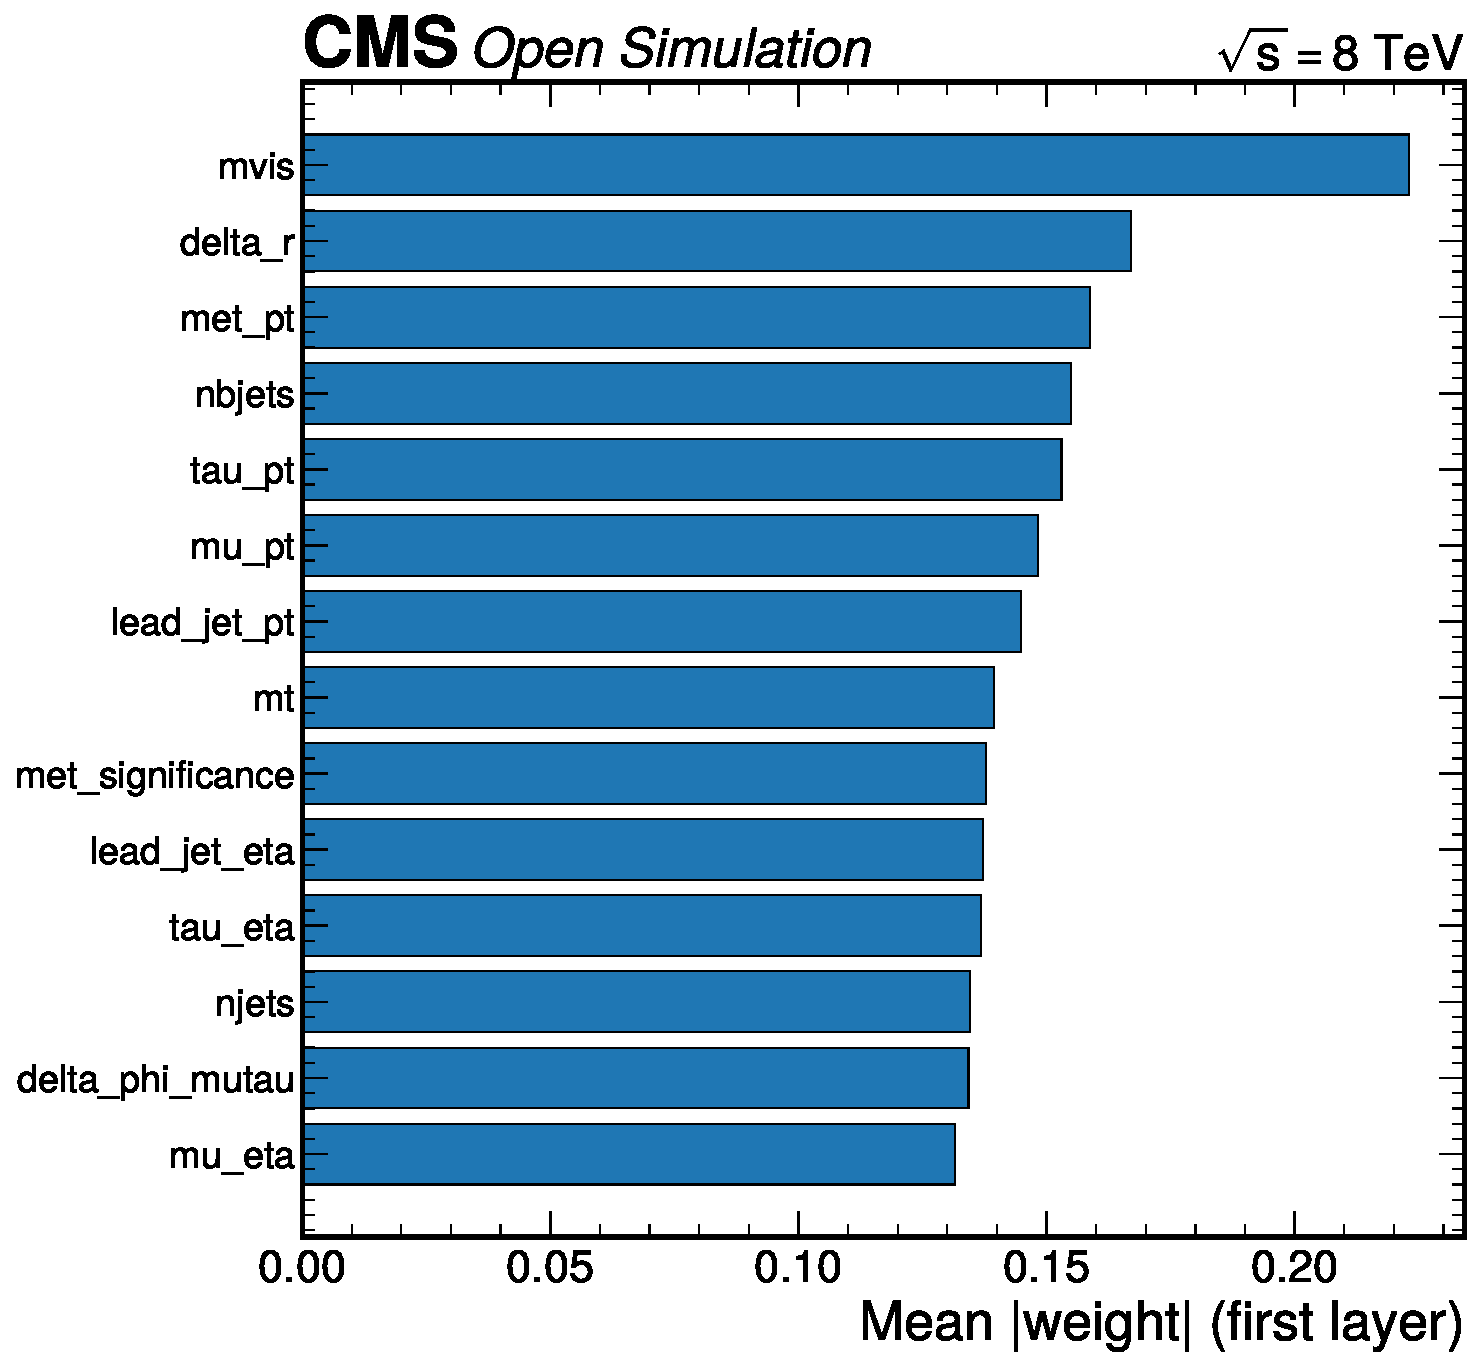
\includegraphics[height=0.35\textheight,width=\linewidth,keepaspectratio,alt={NN input feature importance estimated from the first-layer weight magnitudes. The visible mass (m\_\textbackslash mathrm\{vis\}) is the most important feature, followed by \textbackslash Delta R(\textbackslash mu, \textbackslash tau\_\textbackslash mathrm\{h\}) and E\_\textbackslash mathrm\{T\}\^{}\textbackslash mathrm\{miss\}. The importance ranking generally follows the individual ROC AUC values in tbl.~, with the exception of \textbackslash Delta R which has elevated importance due to its correlation with other kinematic variables.}]{figures/nn_feature_importance.pdf}}
\caption{NN input feature importance estimated from the first-layer
weight magnitudes. The visible mass (\(m_\mathrm{vis}\)) is the most
important feature, followed by \(\Delta R(\mu, \tau_\mathrm{h})\) and
\(E_\mathrm{T}^\mathrm{miss}\). The importance ranking generally follows
the individual ROC AUC values in Table~\ref{tbl:nn-features}, with the
exception of \(\Delta R\) which has elevated importance due to its
correlation with other kinematic variables.}\label{fig:nn-importance}
\end{figure}

\subsubsection{NN input variable quality
gate}\label{nn-input-variable-quality-gate}

Data/MC agreement on all 15 NN input variables was assessed using
\(\chi^2\)/ndf tests in the opposite-sign signal region, including the
QCD template from the same-sign data. The shape-normalized
\(\chi^2\)/ndf (which normalizes MC to data totals to isolate modeling
quality) is the appropriate metric because the overall normalization is
a free parameter in the template fit.

Of the 15 variables, 11 pass the shape \(\chi^2\)/ndf \textless{} 5
gate. Three variables show elevated \(\chi^2\)/ndf values:
\(N_\mathrm{jets}\) (40.68, visible in Figure~\ref{fig:njets-baseline}), \(N_\mathrm{b-jets}\) (32.35), and
\(\Delta R\) (5.16, borderline, Figure~\ref{fig:delta-r-baseline}).
The jet multiplicity mismodeling is a known feature of LO MadGraph
samples and is addressed through per-category normalization nuisance
parameters in the template fit. All three variables are retained because
removing them degrades NN performance, the mismodeling is understood (LO
MC limitations), and the template fit normalization parameters absorb
overall yield differences.

\subsubsection{NN score distributions}\label{nn-score-distributions}

\needspace{0.4\textheight}
\begin{figure}[htbp]
\centering
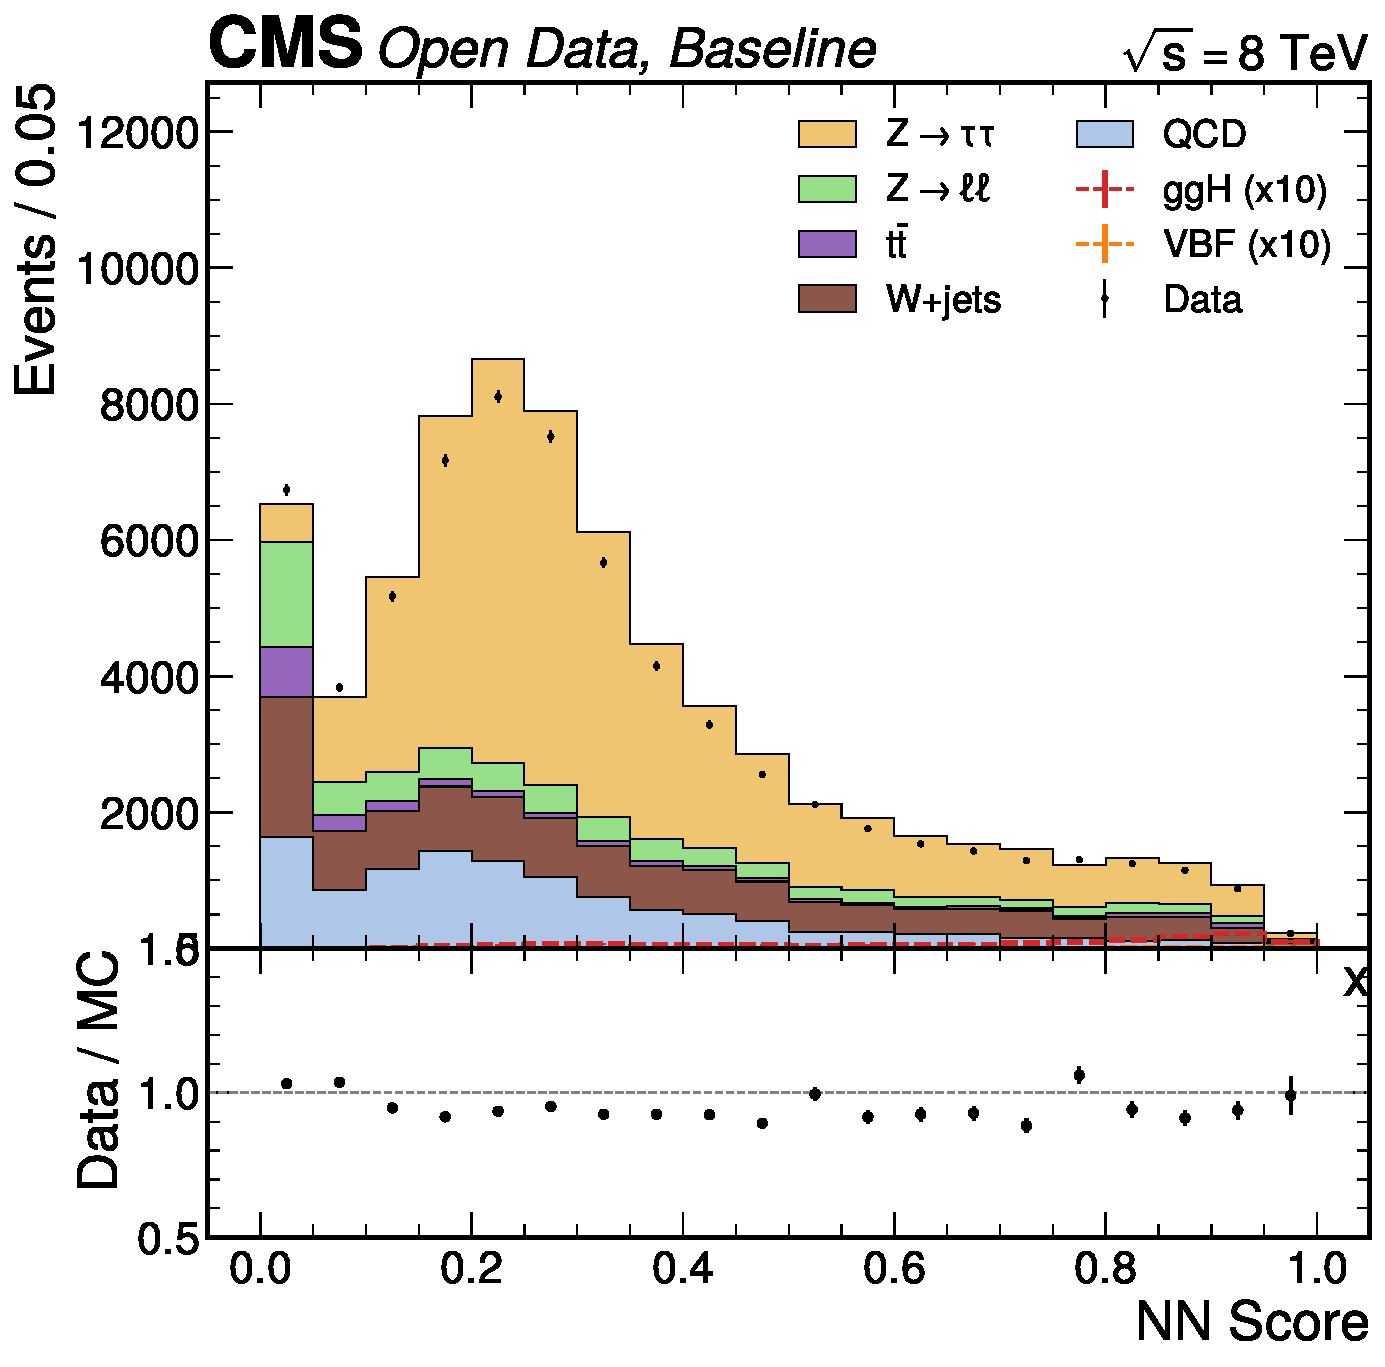
\includegraphics[height=0.38\linewidth,keepaspectratio]{figures/nn_score_baseline.pdf}\hspace{0.02\linewidth}
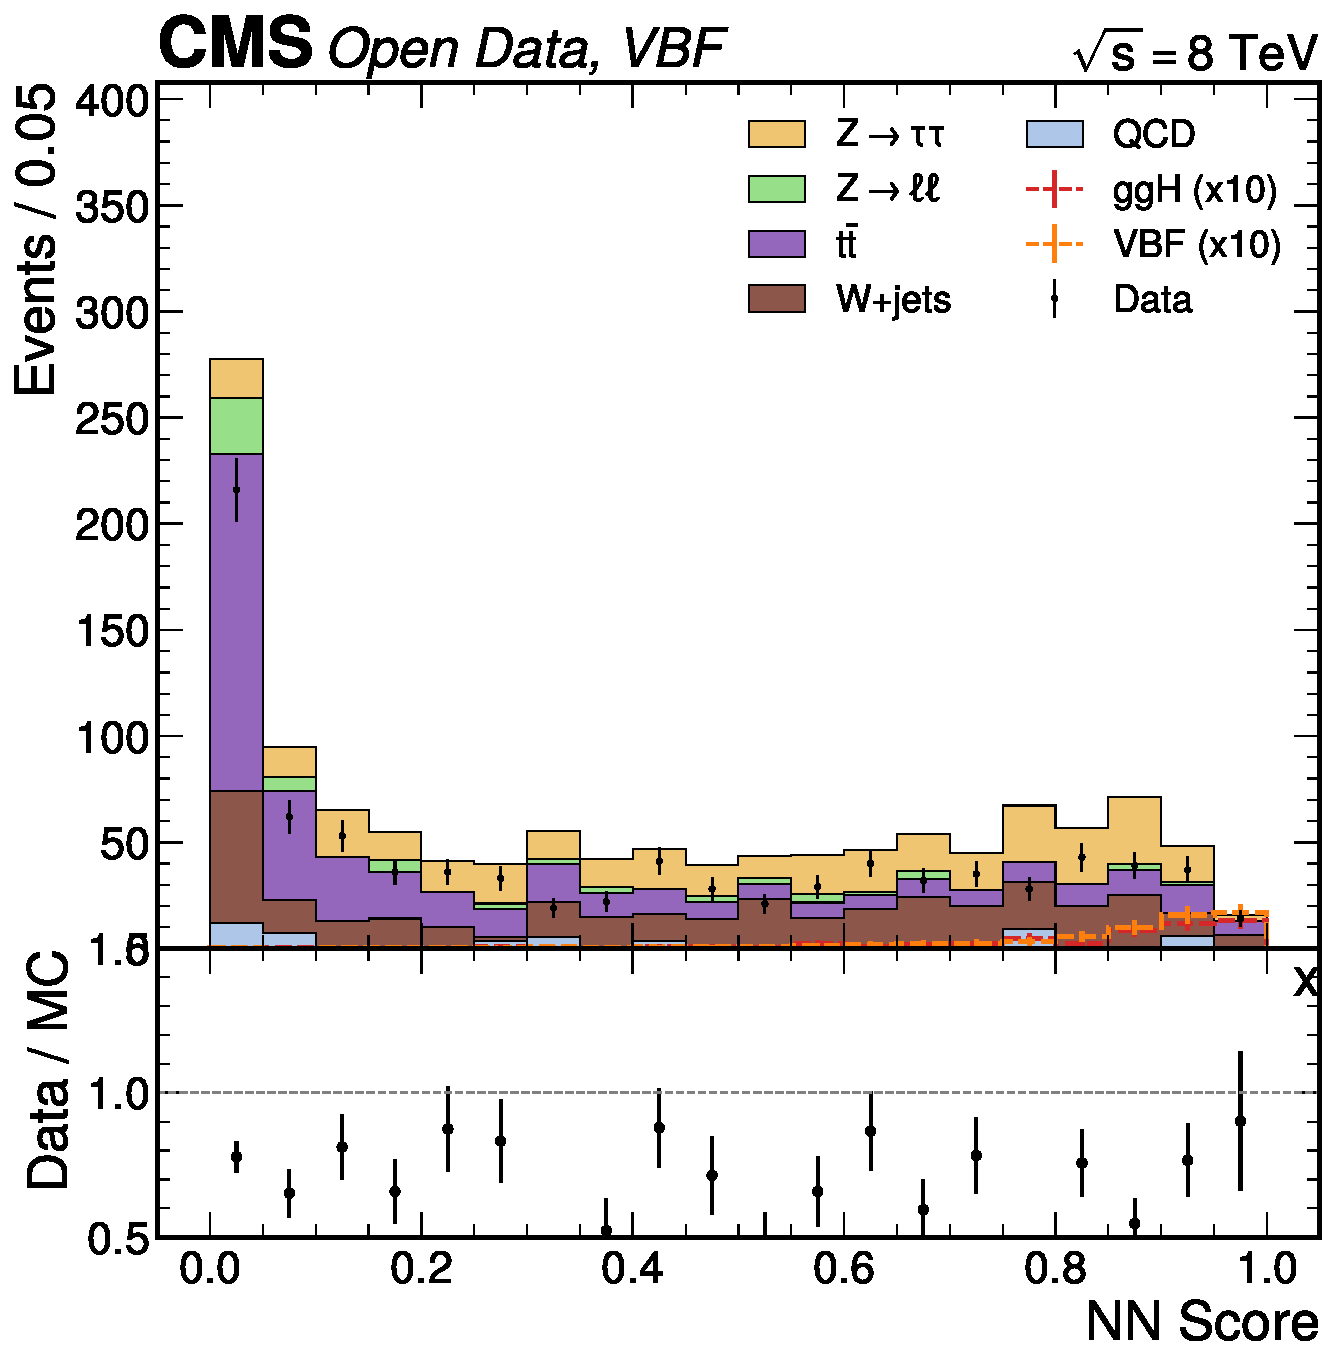
\includegraphics[height=0.38\linewidth,keepaspectratio]{figures/nn_score_vbf.pdf}
\caption{(a) NN discriminant score distribution in the Baseline category.
Background events peak at low NN scores (near 0) while signal events
(shown scaled by x10) peak at high scores (near 1), demonstrating the
discriminating power of the NN classifier. The QCD template is
constructed by evaluating the trained NN on same-sign data events,
ensuring consistent treatment of the data-driven QCD background in the
fitting observable. (b) NN discriminant score distribution in the VBF category. The
separation between signal and background is similar to the Baseline
category, but with reduced statistics. The ratio panel shows larger
fluctuations due to the limited event count in the VBF
category.}\label{fig:nn-score-baseline}
\phantomsection\label{fig:nn-score-vbf}
\end{figure}


\subsubsection{Alternative classifier: BDT
comparison}\label{alternative-classifier-bdt-comparison}

As required by the analysis strategy, a gradient-boosted decision tree
(BDT) classifier was trained as an alternative architecture using the
same features, data split, and weight equalization as the primary NN.
The BDT uses 200 estimators, maximum depth of 3, learning rate of 0.1,
subsample fraction of 0.8, and minimum 50 samples per leaf.

\vspace{1em}
\begin{table}[htbp]
\centering
\small
\caption{Performance comparison between the primary NN and alternative
BDT classifiers. The NN outperforms the BDT by 0.005 AUC on the test
set, with less overtraining.}\label{tbl:bdt-comparison}
\begin{tabular}{@{}
llll@{}}
\toprule\noalign{}
Classifier & AUC (Train) & AUC (Val) & AUC (Test) \\
\midrule\noalign{}
\bottomrule\noalign{}
NN (MLPClassifier) & 0.8426 & 0.8325 & 0.8250 \\
BDT (GradientBoosting) & 0.8752 & 0.8282 & 0.8200 \\
\end{tabular}
\end{table}

The NN outperforms the BDT by 0.005 AUC on the test set (0.825 vs
0.820), as shown in Figure~\ref{fig:bdt-roc}. The BDT shows
slightly more overtraining (train AUC 0.875 vs 0.843 for NN, Figure~\ref{fig:bdt-overtraining}), with the signal KS test \(p\)-value at
0.0007 indicating marginal overtraining. The NN is confirmed as the
better classifier for this analysis.

\needspace{0.4\textheight}
\begin{figure}[htbp]
\centering
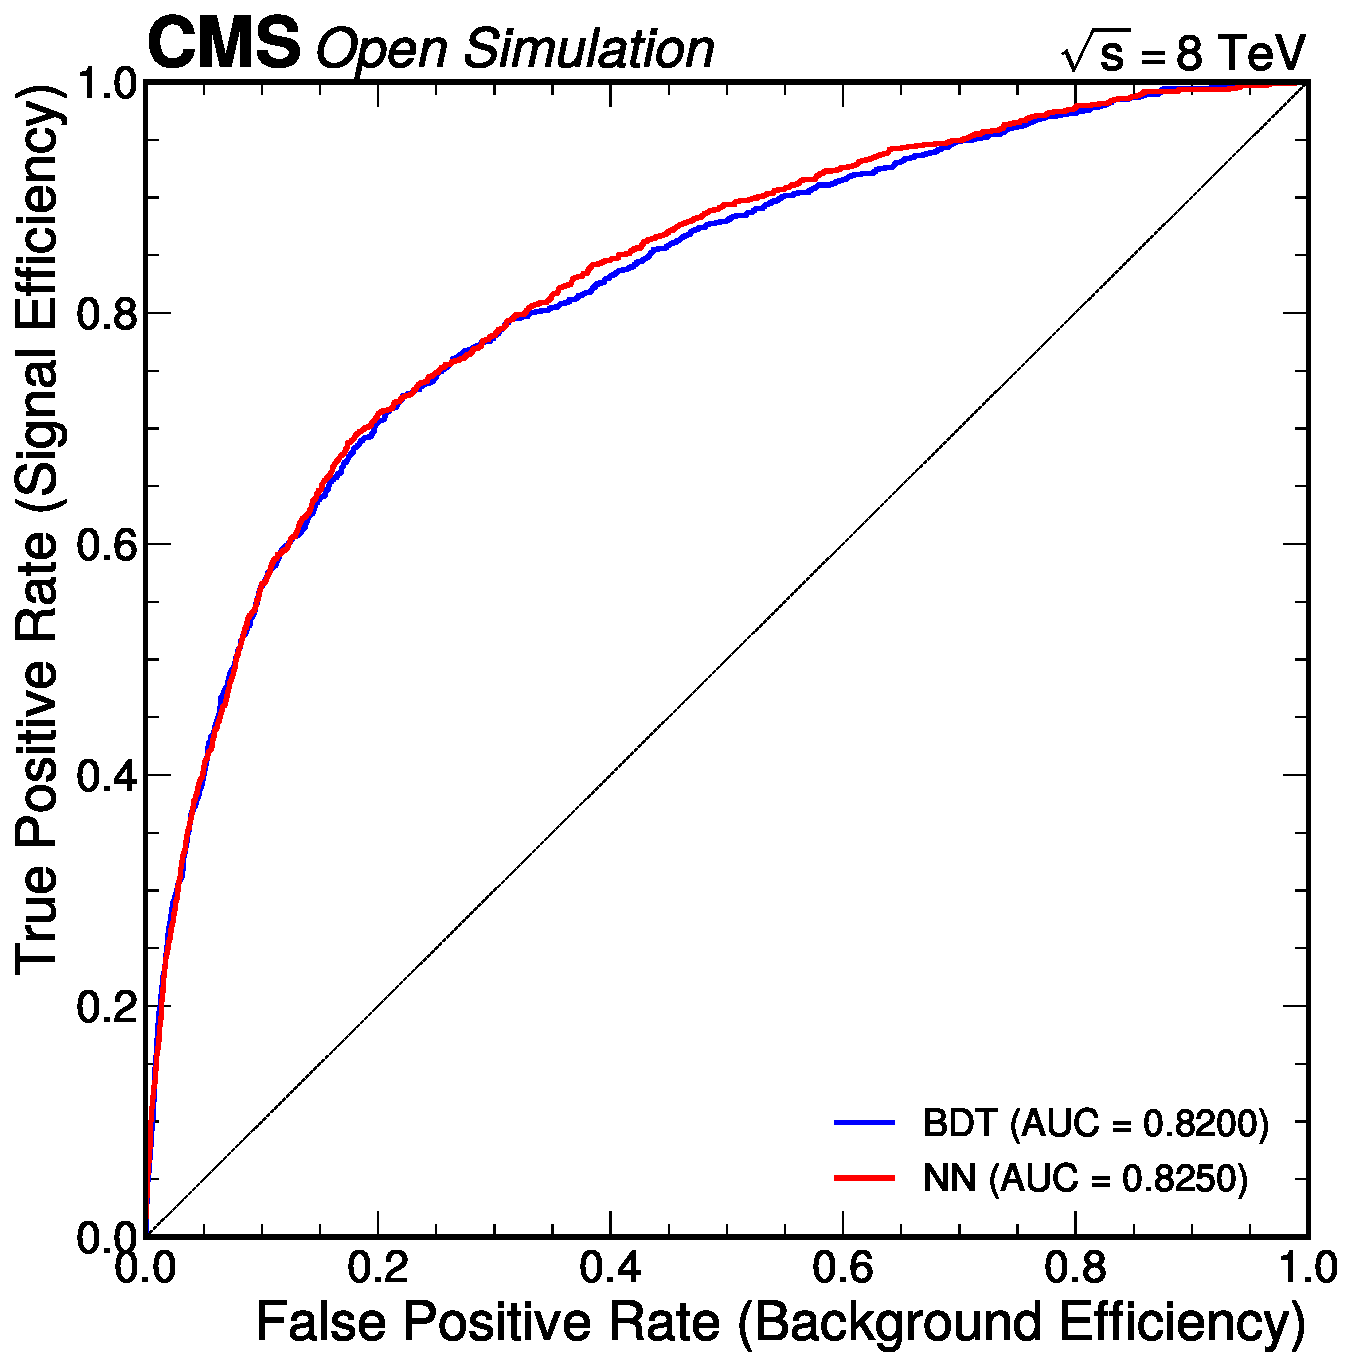
\includegraphics[height=0.38\linewidth,keepaspectratio]{figures/bdt_vs_nn_roc.pdf}\hspace{0.02\linewidth}
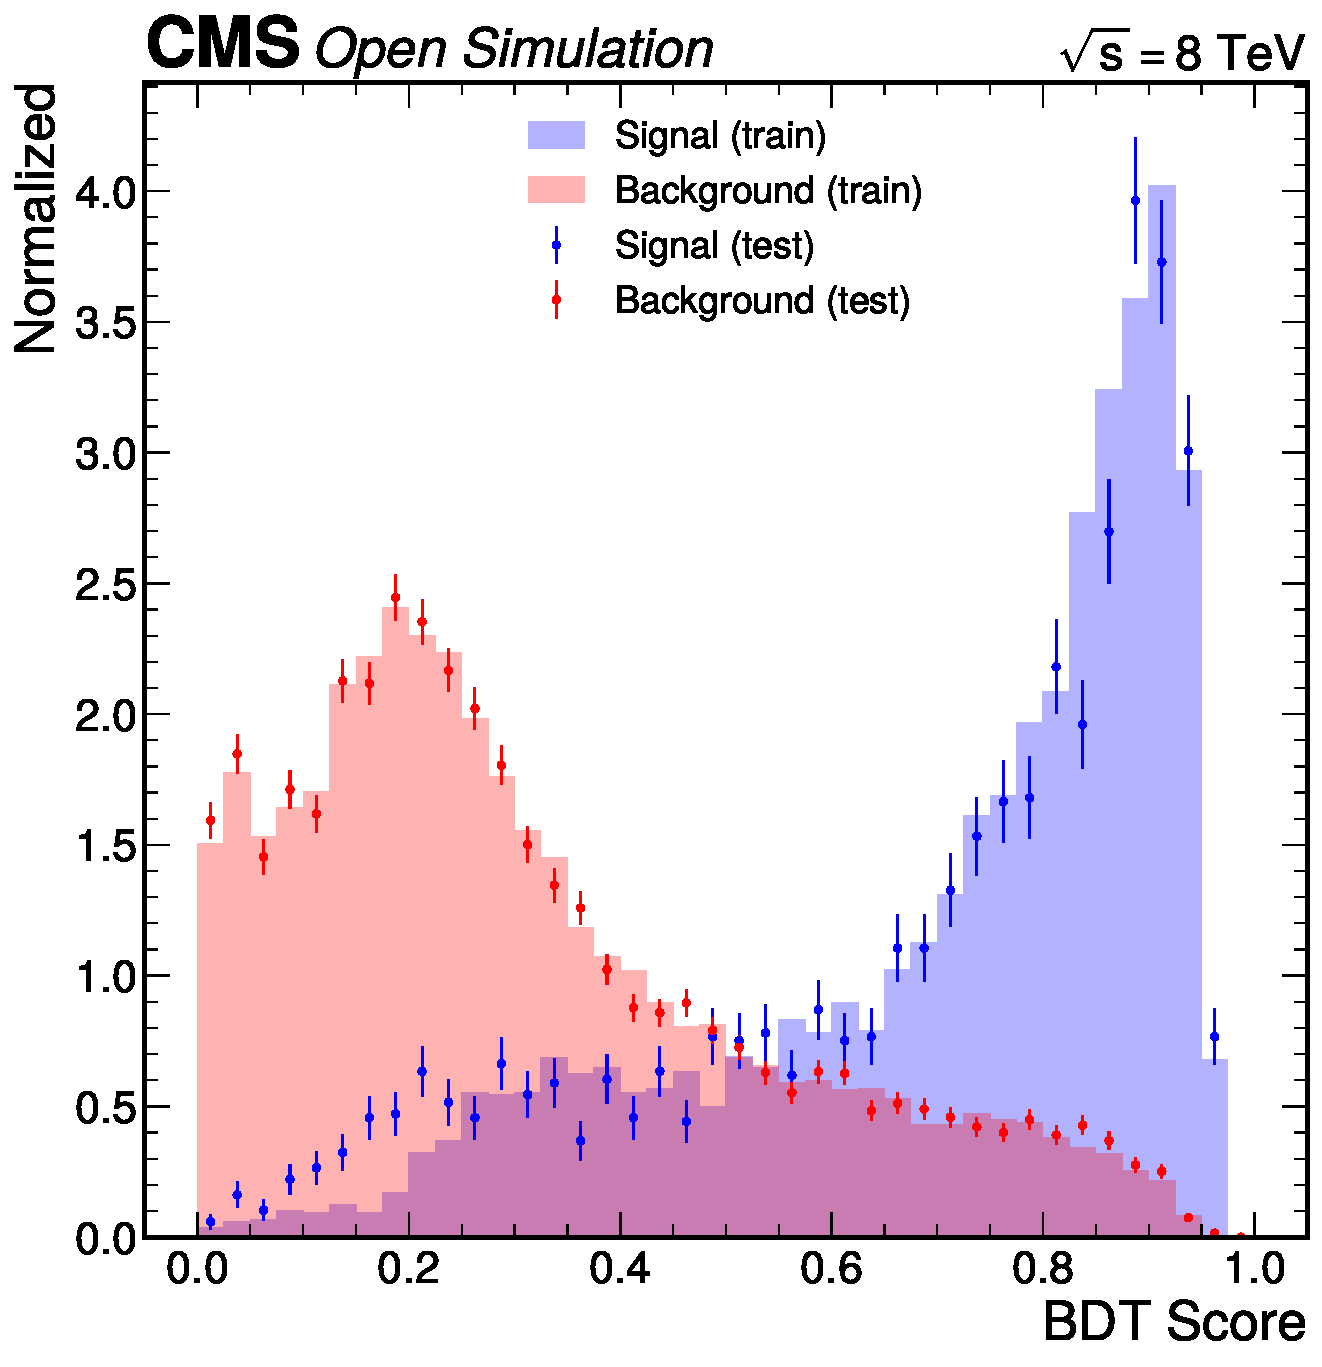
\includegraphics[height=0.38\linewidth,keepaspectratio]{figures/bdt_overtraining.pdf}
\caption{(a) ROC curve comparison between the primary NN classifier and the
alternative BDT. The NN achieves AUC = 0.825 vs BDT AUC = 0.820 on the
test set. The small difference confirms the NN as the preferred
classifier, with the BDT result serving as a cross-check of the MVA
approach. (b) BDT overtraining check. The BDT score distributions overlay
training (filled) and test (points) samples for signal and background.
The signal class shows marginal overtraining (KS \(p\)-value = 0.0007),
with the training distribution shifted slightly toward higher scores
compared to the test distribution. This is consistent with the larger
train-test AUC gap observed for the BDT.}\label{fig:bdt-roc}
\phantomsection\label{fig:bdt-overtraining}
\end{figure}


\needspace{4\baselineskip}
\subsection{Collinear approximation mass}\label{sec:disc-mcol}

The collinear approximation assumes that the neutrinos from tau decays
are collinear with their parent taus, allowing reconstruction of the
full di-tau invariant mass from the visible decay products and the
missing transverse energy. The reconstructed mass is:

\begin{equation}\protect\phantomsection\label{eq:mcol}{m_\mathrm{col} = \frac{m_\mathrm{vis}}{\sqrt{x_\mu \cdot x_\tau}}}\end{equation}

where the momentum fractions are:

\begin{equation}\protect\phantomsection\label{eq:mcol-fractions}{x_\mu = \frac{p_\mathrm{T}^\mu}{p_\mathrm{T}^\mu + p_\mathrm{T}^{\nu_\mu}}, \quad x_\tau = \frac{p_\mathrm{T}^{\tau_\mathrm{h}}}{p_\mathrm{T}^{\tau_\mathrm{h}} + p_\mathrm{T}^{\nu_\tau}}}\end{equation}

The neutrino momenta are obtained by decomposing the MET vector along
the muon and hadronic tau directions. Physical solutions require
\(0 < x_\mu < 1\) and \(0 < x_\tau < 1\). Events with unphysical
solutions use the visible mass as a fallback.

\subsubsection{Physical solution
fractions}\label{physical-solution-fractions}

The unphysical solution fractions, summarized in
Table~\ref{tbl:mcol-physical}, are higher than the strategy estimates but
remain below the 50\% go/no-go threshold for signal events.

\vspace{1em}
\begin{table}[htbp]
\centering
\small
\caption{Physical solution fractions for the collinear approximation.
The ggH signal unphysical fraction of 45.7\% is below the 50\% go/no-go
threshold. Background processes show higher unphysical fractions,
consistent with the collinear assumption being less appropriate for fake
taus and complex final states.}\label{tbl:mcol-physical}
\begin{tabular}{@{}
llll@{}}
\toprule\noalign{}
Sample & Total & Physical & Unphysical fraction \\
\midrule\noalign{}
\bottomrule\noalign{}
ggH & 4,603 & 2,499 & 45.7\% \\
VBF & 6,255 & 3,776 & 39.6\% \\
DY & 34,468 & 16,963 & 50.8\% \\
\(t\bar{t}\) & 5,670 & 2,552 & 55.0\% \\
W+jets (combined) & 11,464 & 4,307 & 62.4\% \\
Data (B+C) & 67,988 & 30,471 & 55.2\% \\
\end{tabular}
\end{table}

The ggH signal has a 45.7\% unphysical fraction, approaching but not
exceeding the 50\% threshold. The VBF signal has a better fraction
(39.6\%) due to its cleaner topology with forward jets. The resulting
collinear mass distributions are shown in Figures~\ref{fig:mcol-baseline} and Figure~\ref{fig:mcol-vbf}. Background
processes show higher unphysical fractions (50-70\%), particularly
\(W\)+jets where the hadronic tau is a misidentified jet with no
physical collinear neutrino. Templates are constructed in 25 bins from 0
to 300 GeV, including both physical and fallback (visible mass)
solutions.

\needspace{0.4\textheight}
\begin{figure}[htbp]
\centering
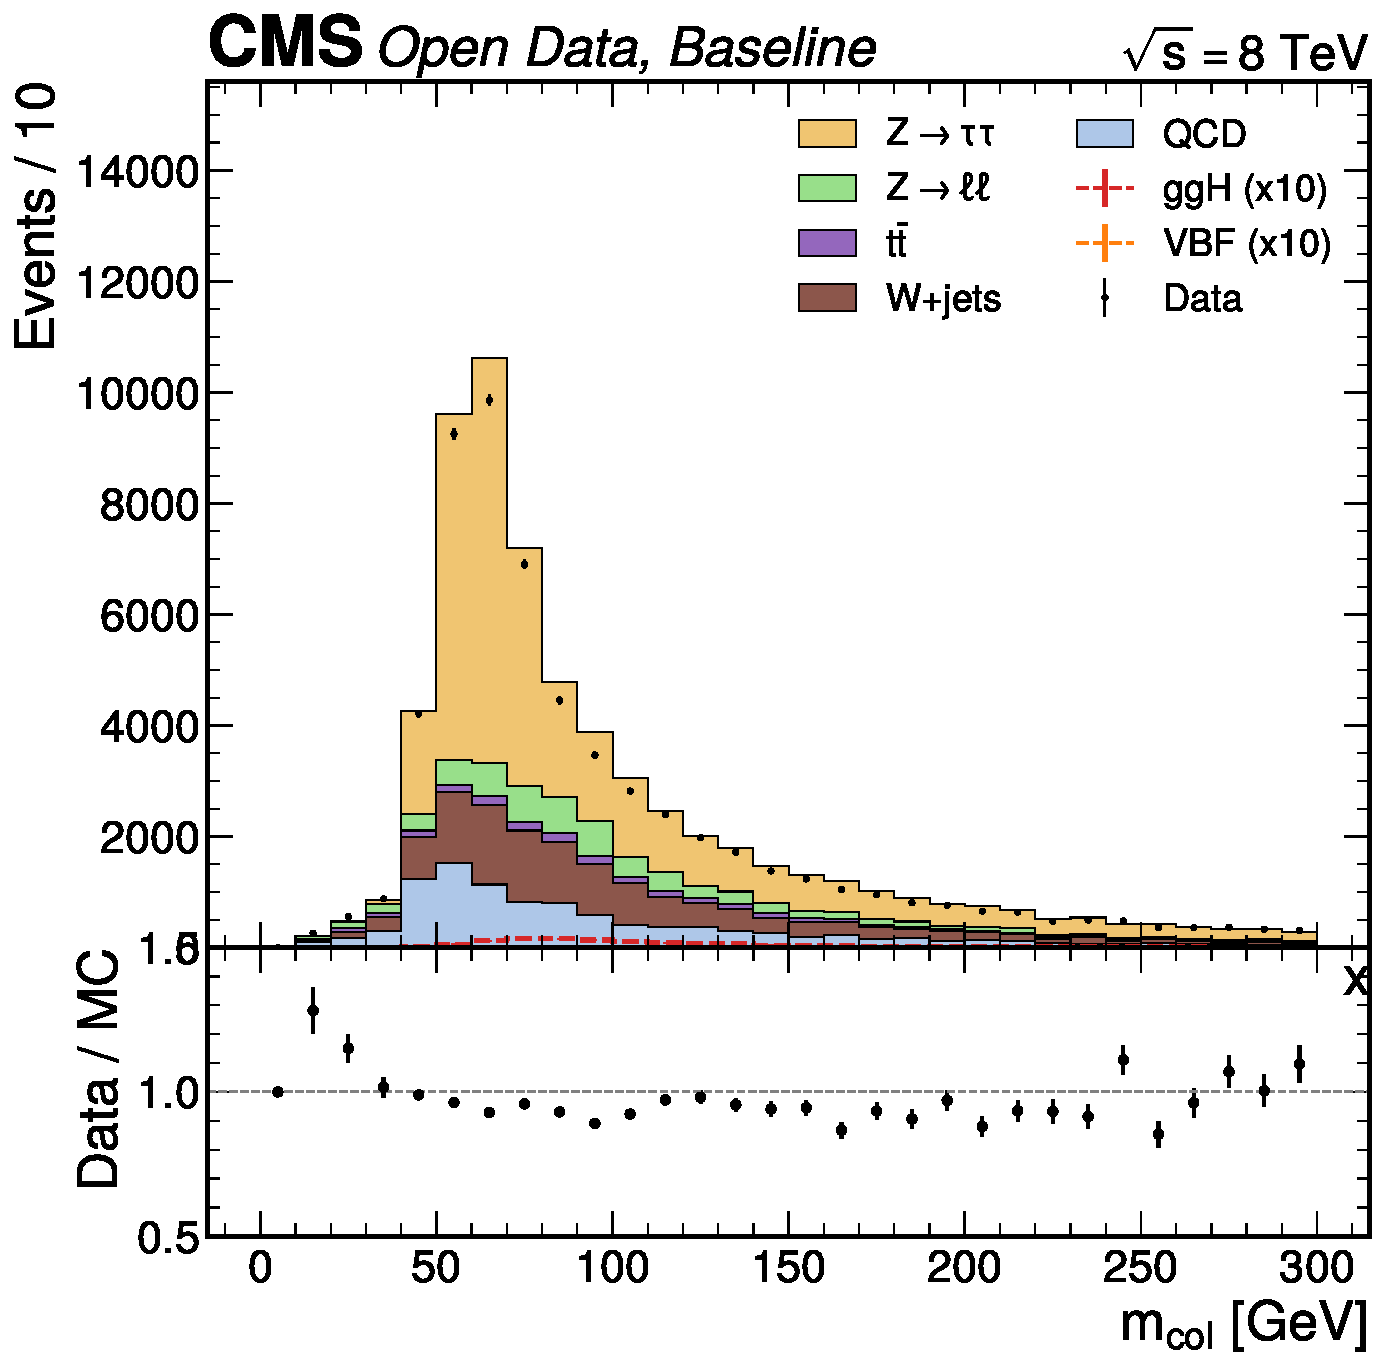
\includegraphics[height=0.38\linewidth,keepaspectratio]{figures/mcol_baseline.pdf}\hspace{0.02\linewidth}
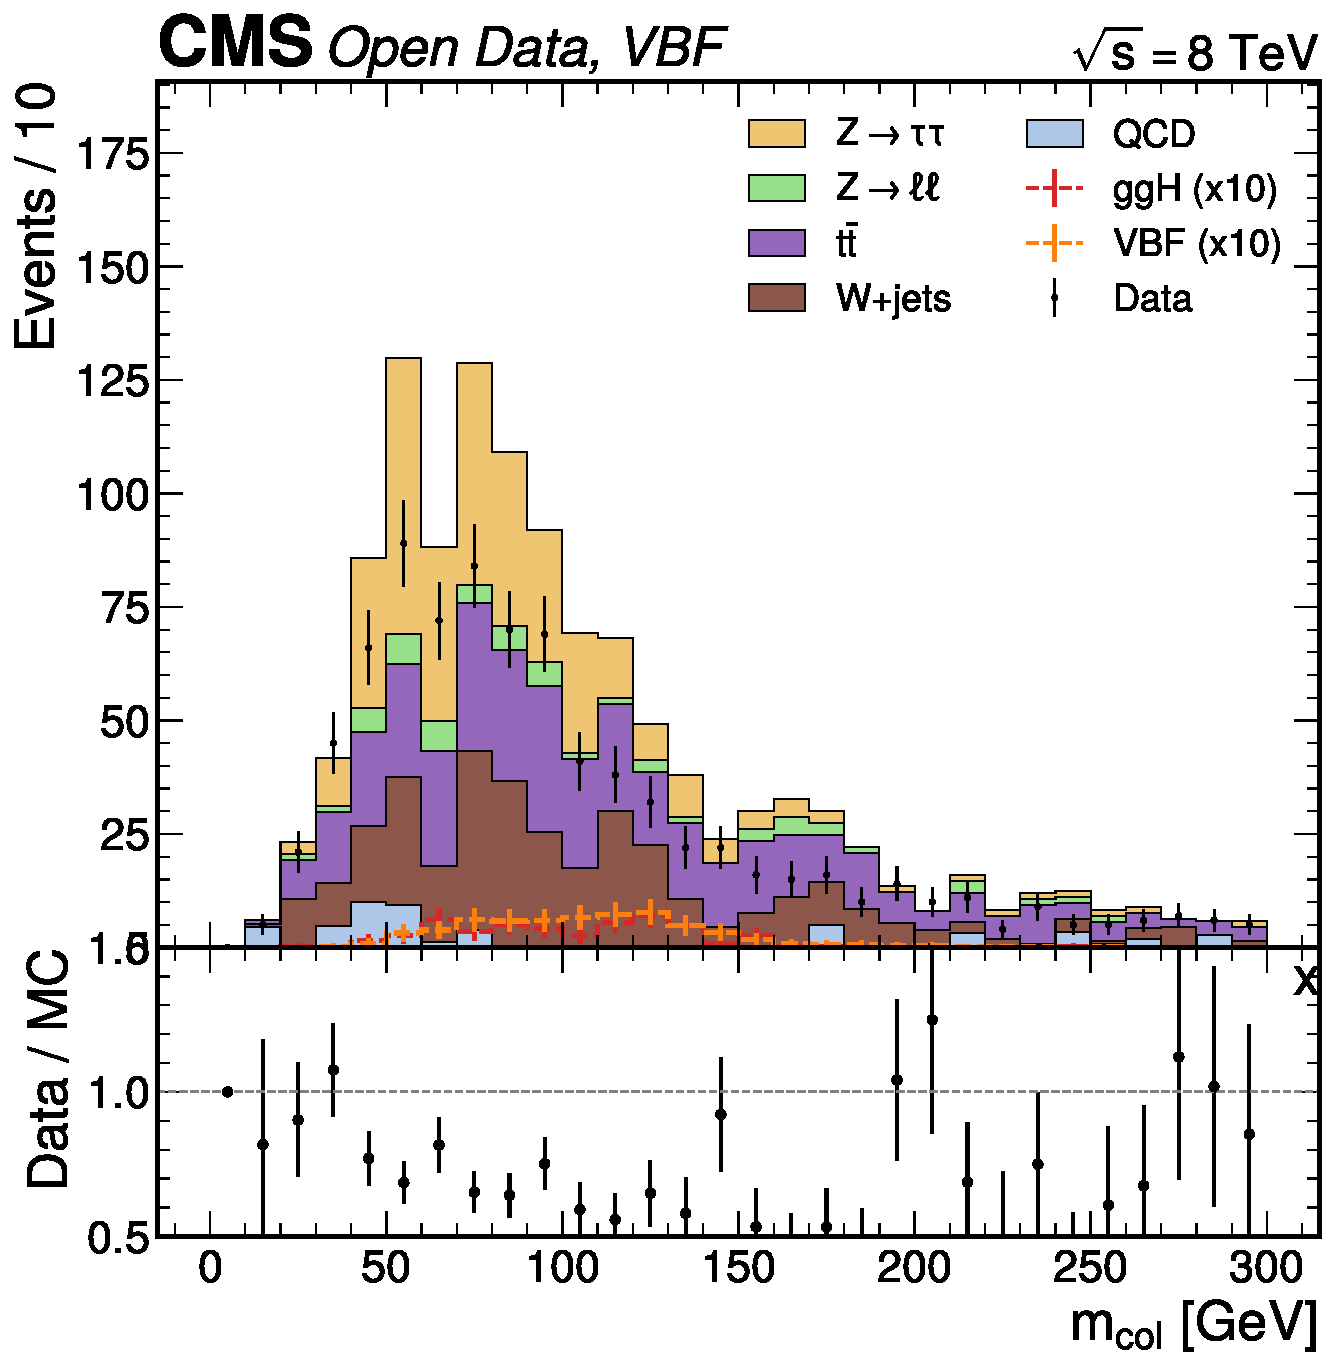
\includegraphics[height=0.38\linewidth,keepaspectratio]{figures/mcol_vbf.pdf}
\caption{(a) Collinear mass distribution in the Baseline category. The QCD
template is computed from the collinear mass values of same-sign events,
ensuring consistency with the fitting observable. The broader
distribution compared to the visible mass reflects the inclusion of
unphysical collinear solutions that fall back to the visible mass.
Events with physical solutions produce the characteristic peaks at the Z
and Higgs masses. (b) Collinear mass distribution in the VBF category. The reduced
statistics and higher unphysical fractions for background processes make
this observable less powerful in the VBF category. Nevertheless, the
collinear mass provides complementary information to the visible mass
through the improved mass resolution for events with physical
solutions.}\label{fig:mcol-baseline}
\phantomsection\label{fig:mcol-vbf}
\end{figure}


\needspace{4\baselineskip}
\subsection{Approach comparison}\label{sec:disc-comparison}

The three fitting approaches are compared using the expected
significance metric, computed consistently with the data-driven QCD
background included in all approaches:

\vspace{1em}
\begin{table}[htbp]
\centering
\small
\caption{Comparison of the three fitting approaches. The NN discriminant
provides the best expected significance, improving over the visible mass
baseline by 89\% and over the collinear mass by a factor of 2.2. These
pre-fit estimates use a simple \(S/\sqrt{B}\) counting metric; the
profile likelihood fit results are presented in Section~\ref{sec:expected-results}.}\label{tbl:approach-comparison}
\begin{tabular}{@{}
>{\raggedright\arraybackslash}p{(\linewidth - 4\tabcolsep) * \real{0.1613}}
  >{\raggedright\arraybackslash}p{(\linewidth - 4\tabcolsep) * \real{0.4677}}
  >{\raggedright\arraybackslash}p{(\linewidth - 4\tabcolsep) * \real{0.3710}}@{}}
\toprule\noalign{}
\begin{minipage}[b]{\linewidth}\raggedright
Approach
\end{minipage} & \begin{minipage}[b]{\linewidth}\raggedright
\(S/\sqrt{B}\) (signal window)
\end{minipage} & \begin{minipage}[b]{\linewidth}\raggedright
Expected significance
\end{minipage} \\
\midrule\noalign{}
\toprule\noalign{}
\begin{minipage}[b]{\linewidth}\raggedright
Approach
\end{minipage} & \begin{minipage}[b]{\linewidth}\raggedright
\(S/\sqrt{B}\) (signal window)
\end{minipage} & \begin{minipage}[b]{\linewidth}\raggedright
Expected significance
\end{minipage} \\
\midrule\noalign{}
\bottomrule\noalign{}
Visible mass (\(m_\mathrm{vis}\)) & 0.144 (100-150 GeV) &
0.80\(\sigma\) \\
\textbf{NN discriminant} & \textbf{1.251 (score \textgreater{} 0.8)} &
\textbf{1.52\(\sigma\)} \\
Collinear mass (\(m_\mathrm{col}\)) & 0.426 (110-160 GeV) &
0.68\(\sigma\) \\
\end{tabular}
\end{table}

The NN discriminant is selected as the primary fitting observable based
on its substantially better expected sensitivity (Figure~\ref{fig:approach-comparison}). The visible mass and collinear mass
are retained as cross-check approaches. The full profile likelihood
results confirm these pre-fit estimates (Section~\ref{sec:expected-results}).

\needspace{0.4\textheight}
\begin{figure}[htbp]
\centering
\pandocbounded{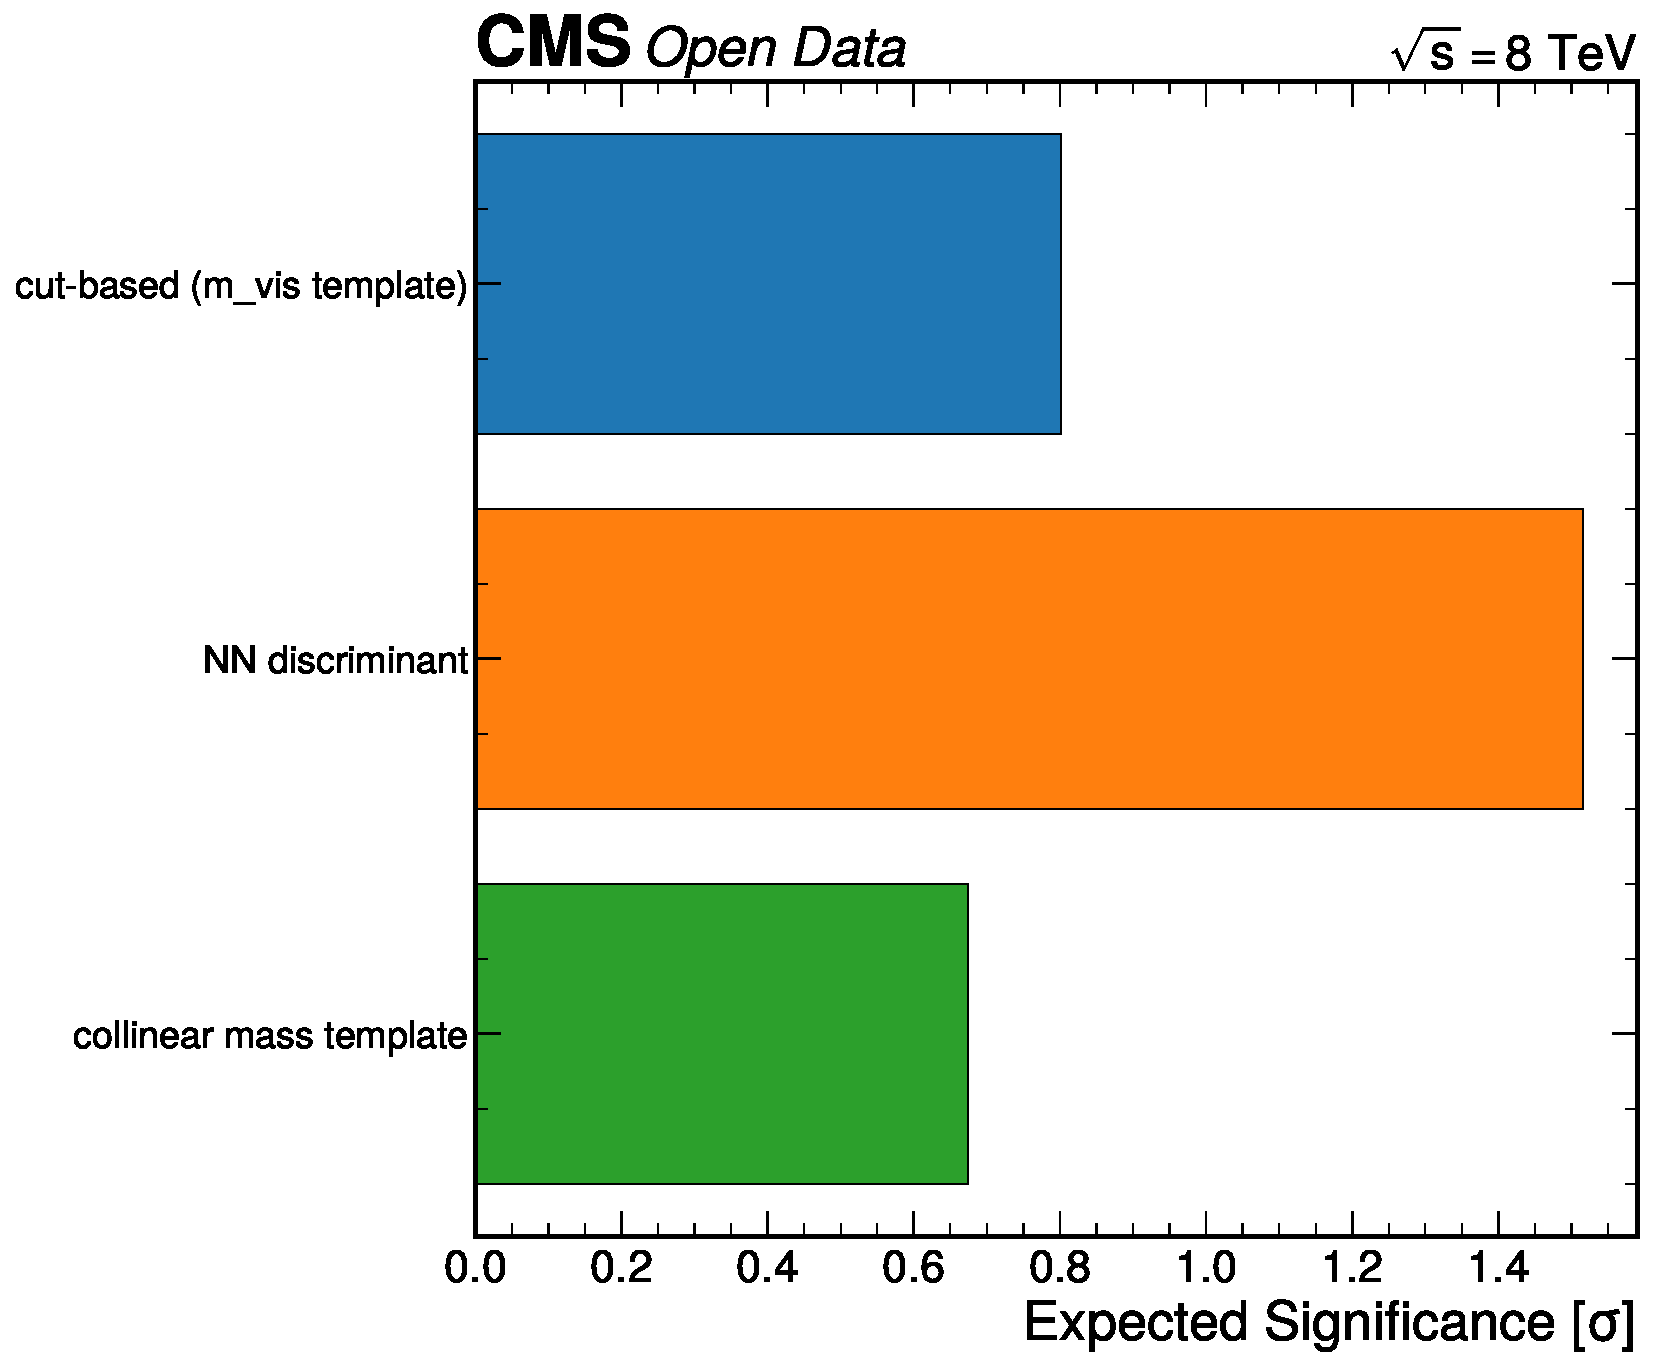
\includegraphics[height=0.35\textheight,width=\linewidth,keepaspectratio,alt={Comparison of expected significance across the three fitting approaches: visible mass template (m\_\textbackslash mathrm\{vis\}), neural network discriminant (NN score), and collinear approximation mass (m\_\textbackslash mathrm\{col\}). All approaches include consistent treatment of the data-driven QCD background. The NN discriminant provides the best expected significance at 1.52\textbackslash sigma, representing an 89\% improvement over the cut-based visible mass approach.}]{figures/approach_comparison.pdf}}
\caption{Comparison of expected significance across the three fitting
approaches: visible mass template (\(m_\mathrm{vis}\)), neural network
discriminant (NN score), and collinear approximation mass
(\(m_\mathrm{col}\)). All approaches include consistent treatment of the
data-driven QCD background. The NN discriminant provides the best
expected significance at 1.52\(\sigma\), representing an 89\%
improvement over the cut-based visible mass
approach.}\label{fig:approach-comparison}
\end{figure}

\needspace{4\baselineskip}
\FloatBarrier
\section{Kinematic Distributions}\label{sec:kinematics}

This section presents the data/MC comparison for key kinematic
distributions in the Baseline and VBF categories. All distributions
include the data-driven QCD estimate from the same-sign region and the
\(W\)+jets scale factor correction. These comparisons validate the
modeling of the input variables that enter the NN discriminant and the
fitting observables. The individual variable separation powers are
summarized in Figure~\ref{fig:separation-power}.

\needspace{4\baselineskip}
\subsection{Baseline category distributions}\label{sec:kin-baseline}

\needspace{0.4\textheight}
\begin{figure}[htbp]
\centering
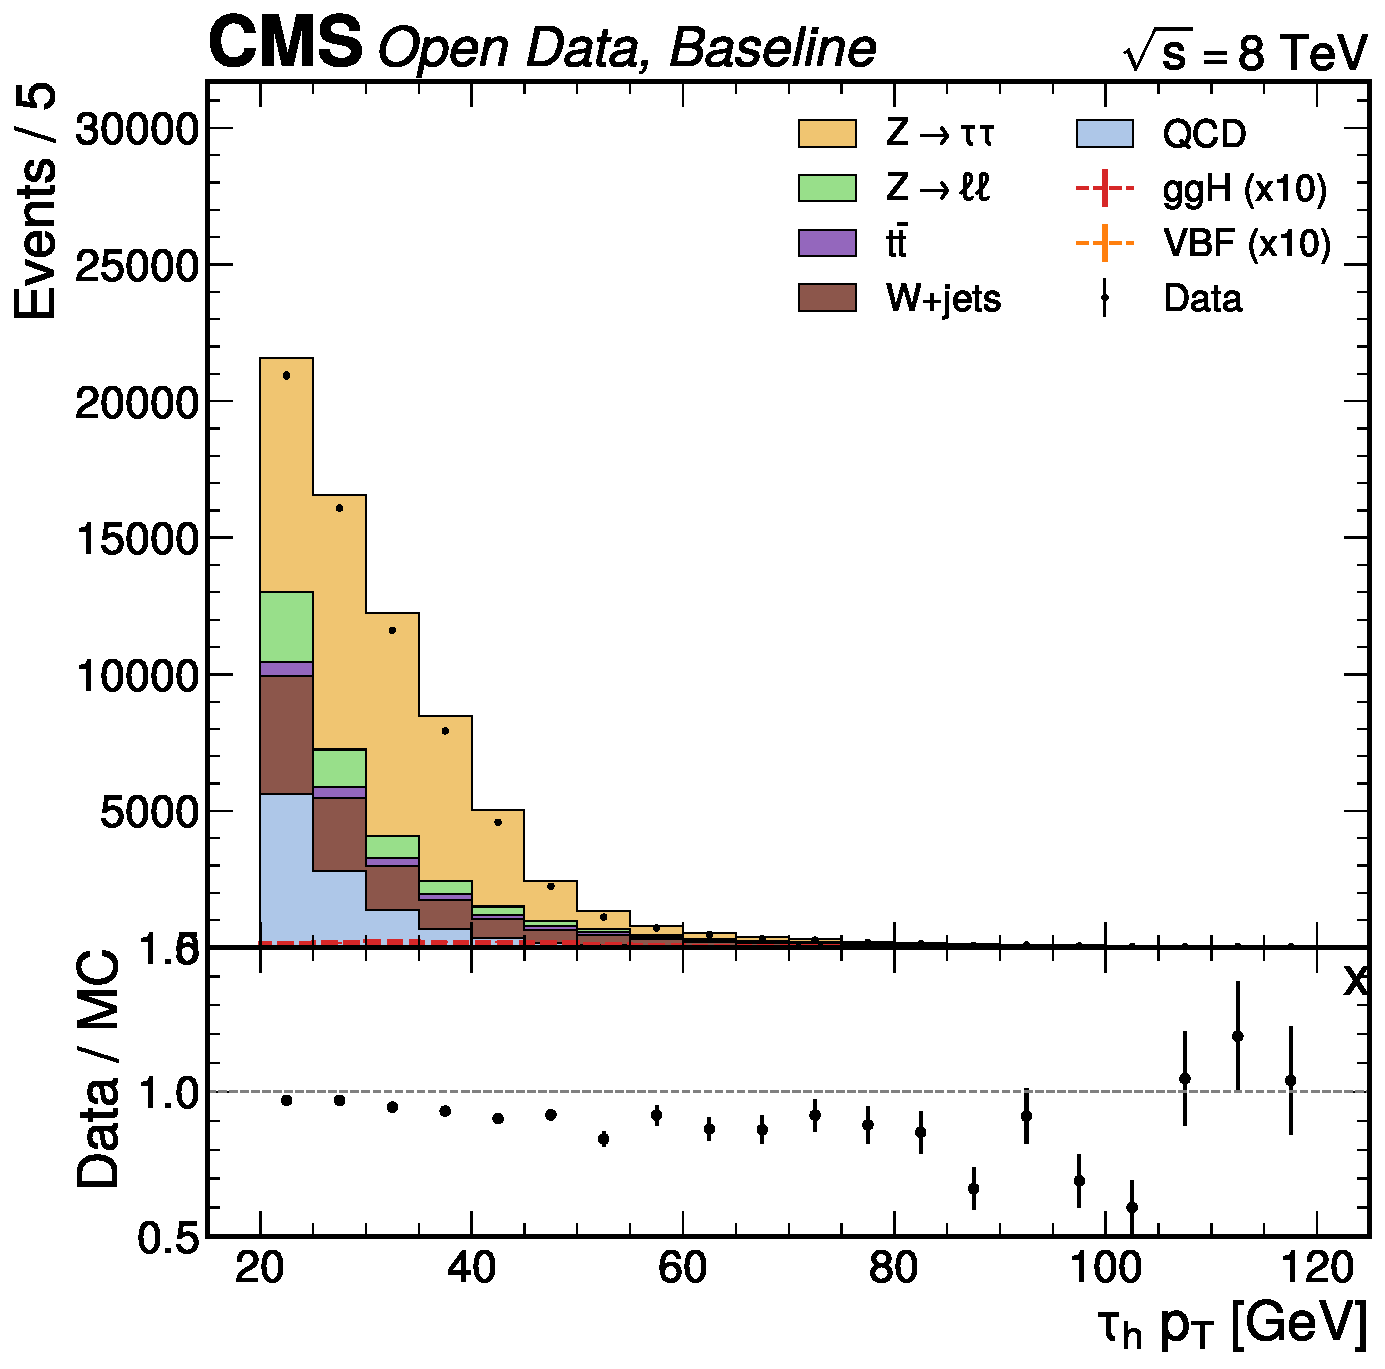
\includegraphics[height=0.38\linewidth,keepaspectratio]{figures/tau_pt_baseline.pdf}\hspace{0.02\linewidth}
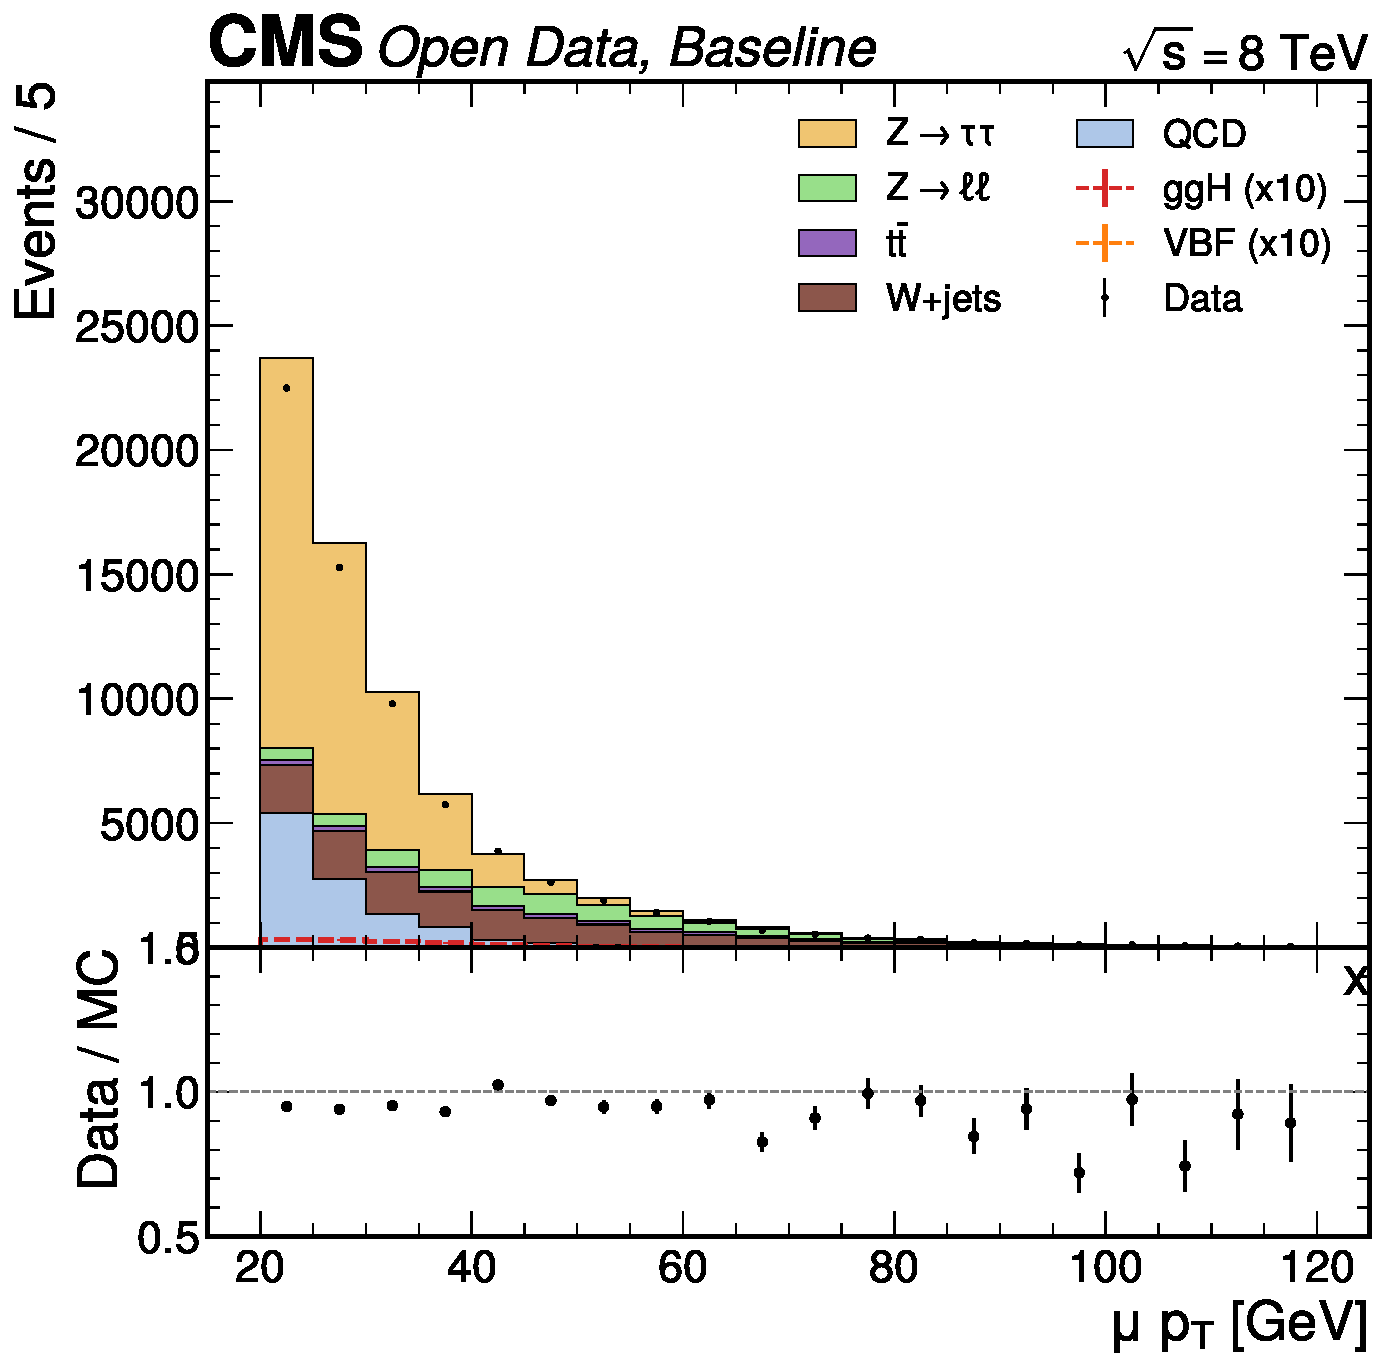
\includegraphics[height=0.38\linewidth,keepaspectratio]{figures/mu_pt_baseline.pdf}
\caption{(a) Hadronic tau \(p_\mathrm{T}\) distribution in the Baseline
category. The steeply falling spectrum is well modeled by the MC
simulation. The tau \(p_\mathrm{T}\) is the most discriminating
individual variable (ROC AUC = 0.695), as signal taus from Higgs decay
tend to have harder \(p_\mathrm{T}\) spectra than those from \(Z\) decay
due to the higher parent mass. (b) Muon \(p_\mathrm{T}\) distribution in the Baseline category.
The distribution peaks near the 20 GeV selection threshold, with the MC
prediction showing reasonable agreement with data. The slight excess in
data at high \(p_\mathrm{T}\) is consistent with the QCD multijet
contribution, which tends to produce higher-\(p_\mathrm{T}\) muons than
the \(Z\to\tau\tau\) background.}\label{fig:tau-pt-baseline}
\phantomsection\label{fig:mu-pt-baseline}
\end{figure}


\needspace{0.4\textheight}
\begin{figure}[htbp]
\centering
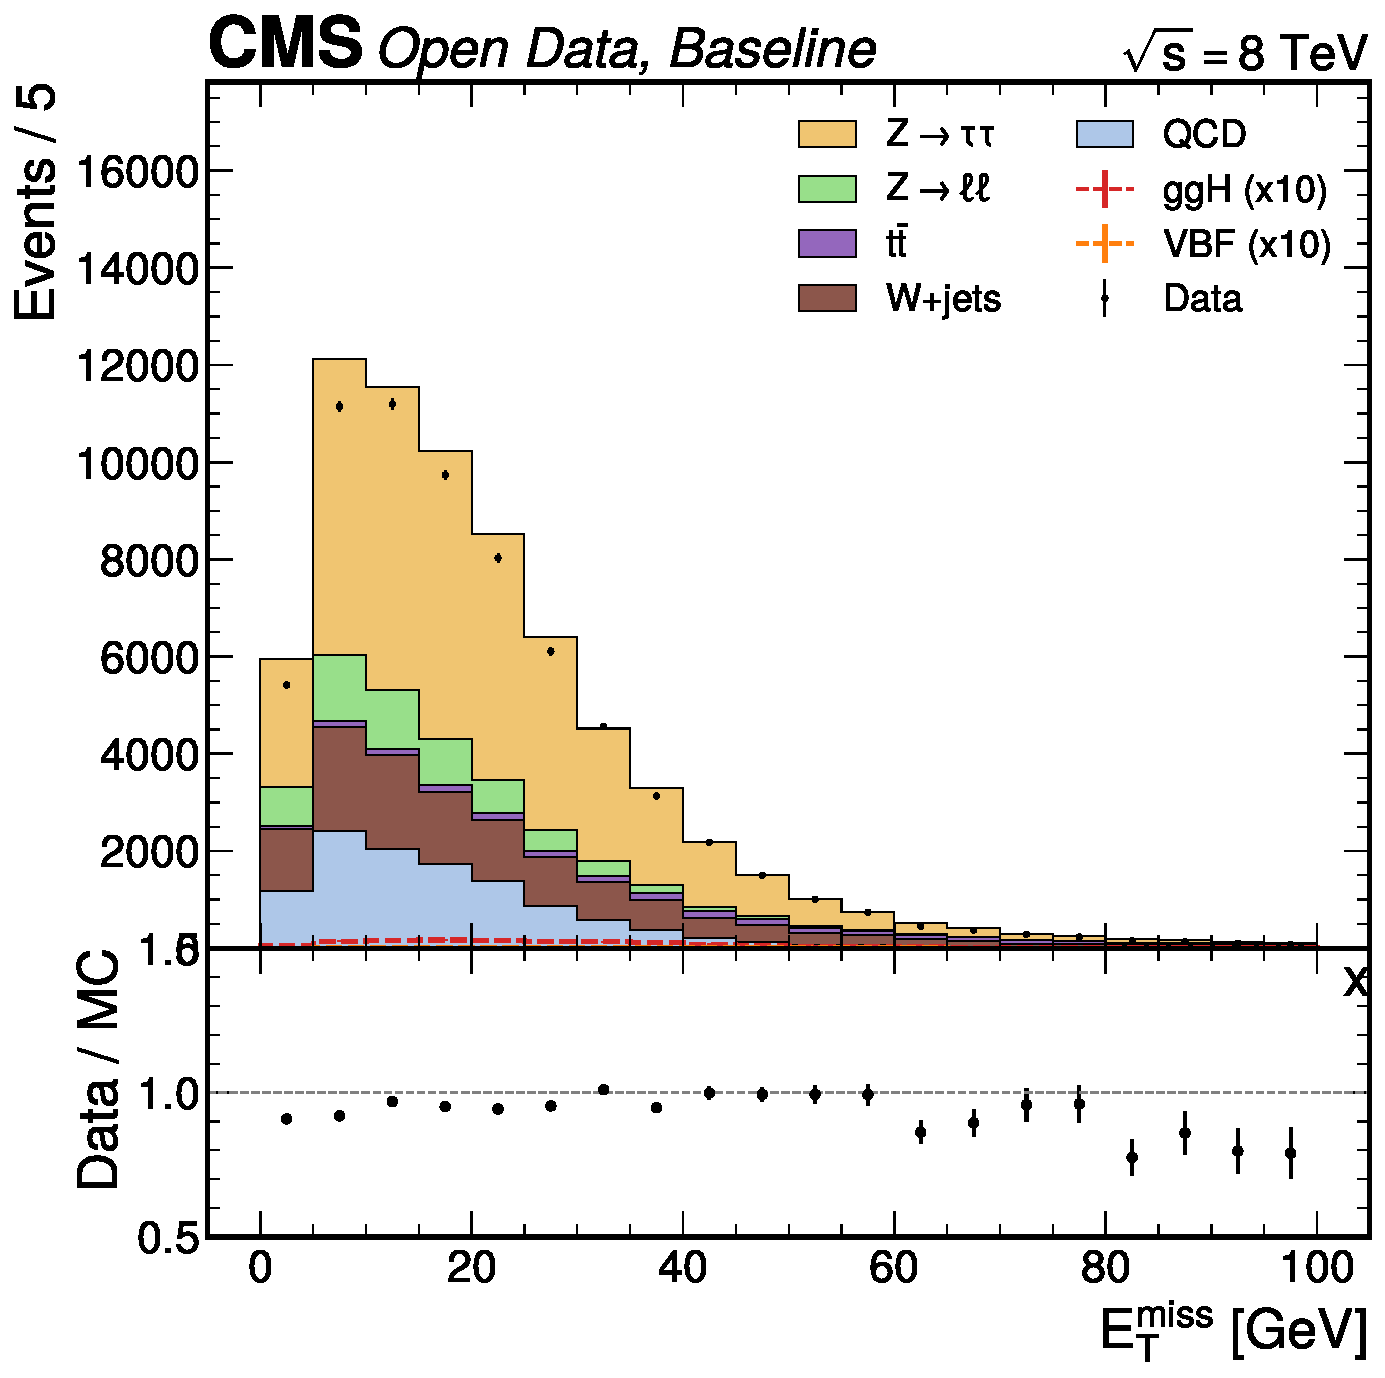
\includegraphics[height=0.38\linewidth,keepaspectratio]{figures/met_pt_baseline.pdf}\hspace{0.02\linewidth}
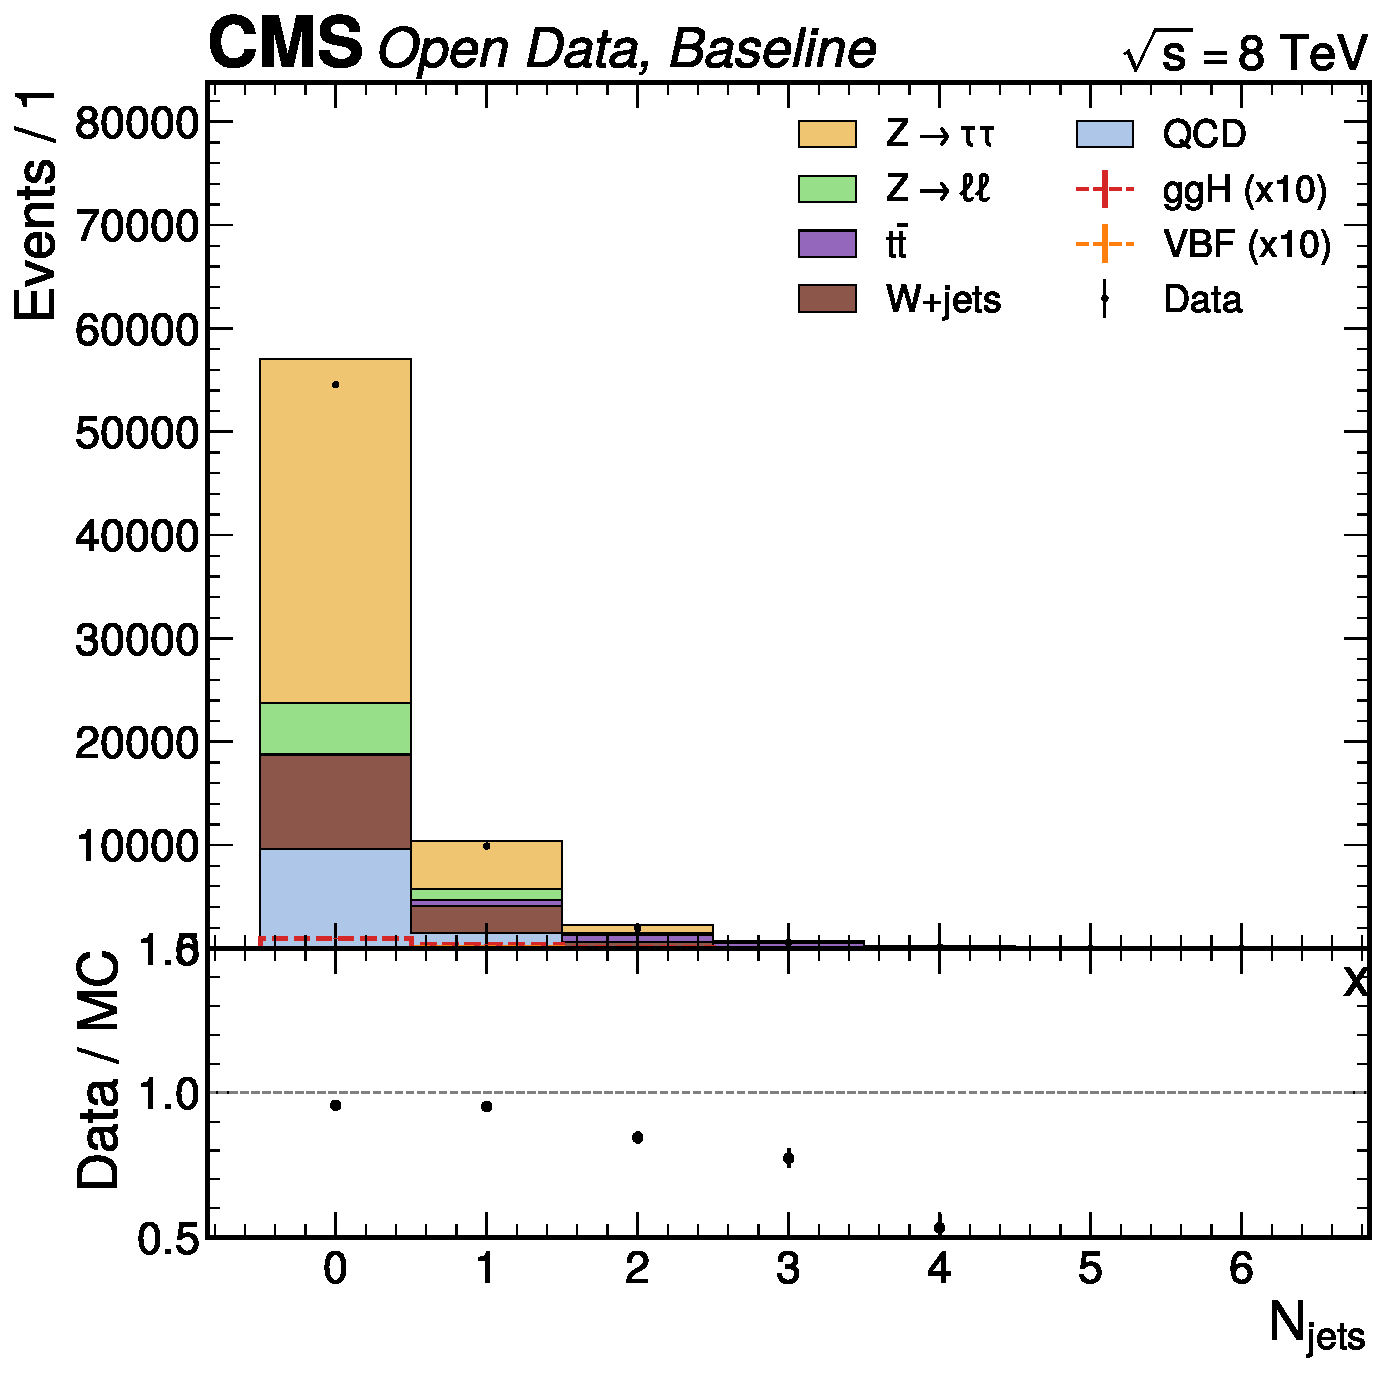
\includegraphics[height=0.38\linewidth,keepaspectratio]{figures/njets_baseline.pdf}
\caption{(a) Missing transverse energy (\(E_\mathrm{T}^\mathrm{miss}\))
distribution in the Baseline category. The data shows slightly higher
MET than the MC prediction, consistent with the QCD multijet
contribution. The MET is the fourth most discriminating variable (ROC
AUC = 0.639), as the additional neutrinos from the Higgs decay produce
more MET than the \(Z\to\tau\tau\) background. (b) Jet multiplicity distribution in the Baseline category. The LO
MadGraph MC shows known mismodeling at high jet multiplicities
(\(N_\mathrm{jets} \geq 2\)), where the data exceeds the prediction.
This is a well-documented feature of LO generators and is addressed in
the statistical model through per-category normalization nuisance
parameters.}\label{fig:met-baseline}
\phantomsection\label{fig:njets-baseline}
\end{figure}


\needspace{0.4\textheight}
\begin{figure}[htbp]
\centering
\pandocbounded{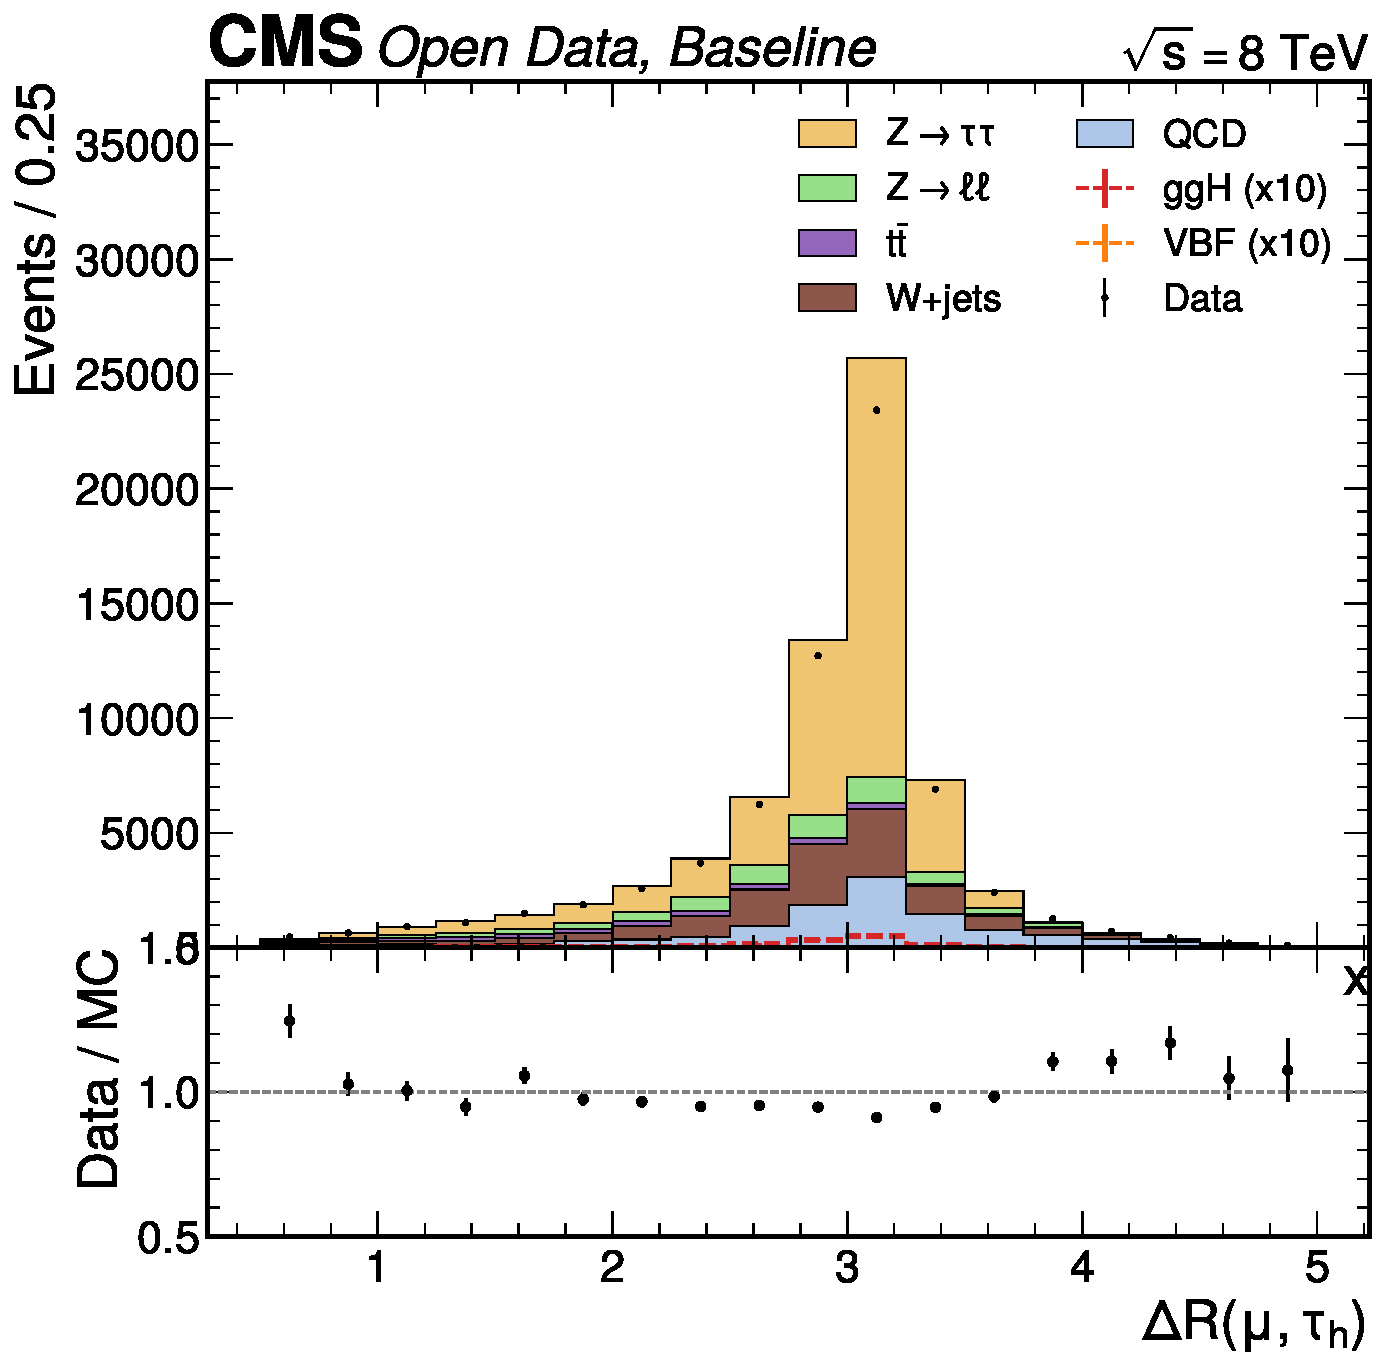
\includegraphics[height=0.35\textheight,width=\linewidth,keepaspectratio,alt={Angular separation \textbackslash Delta R(\textbackslash mu, \textbackslash tau\_\textbackslash mathrm\{h\}) in the Baseline category. The distribution peaks near \textbackslash pi, consistent with the back-to-back topology expected from Z/H \textbackslash to \textbackslash tau\textbackslash tau decays where the two tau leptons are produced approximately opposite in azimuth. The data/MC agreement is generally good, with a slight excess at large separations (\textbackslash Delta R \textgreater{} 3.5) attributed to QCD multijet events.}]{figures/delta_r_baseline.pdf}}
\caption{Angular separation \(\Delta R(\mu, \tau_\mathrm{h})\) in the
Baseline category. The distribution peaks near \(\pi\), consistent with
the back-to-back topology expected from \(Z/H \to \tau\tau\) decays
where the two tau leptons are produced approximately opposite in
azimuth. The data/MC agreement is generally good, with a slight excess
at large separations (\(\Delta R > 3.5\)) attributed to QCD multijet
events.}\label{fig:delta-r-baseline}
\end{figure}

\needspace{4\baselineskip}
\subsection{VBF category distributions}\label{sec:kin-vbf}

\needspace{0.4\textheight}
\begin{figure}[htbp]
\centering
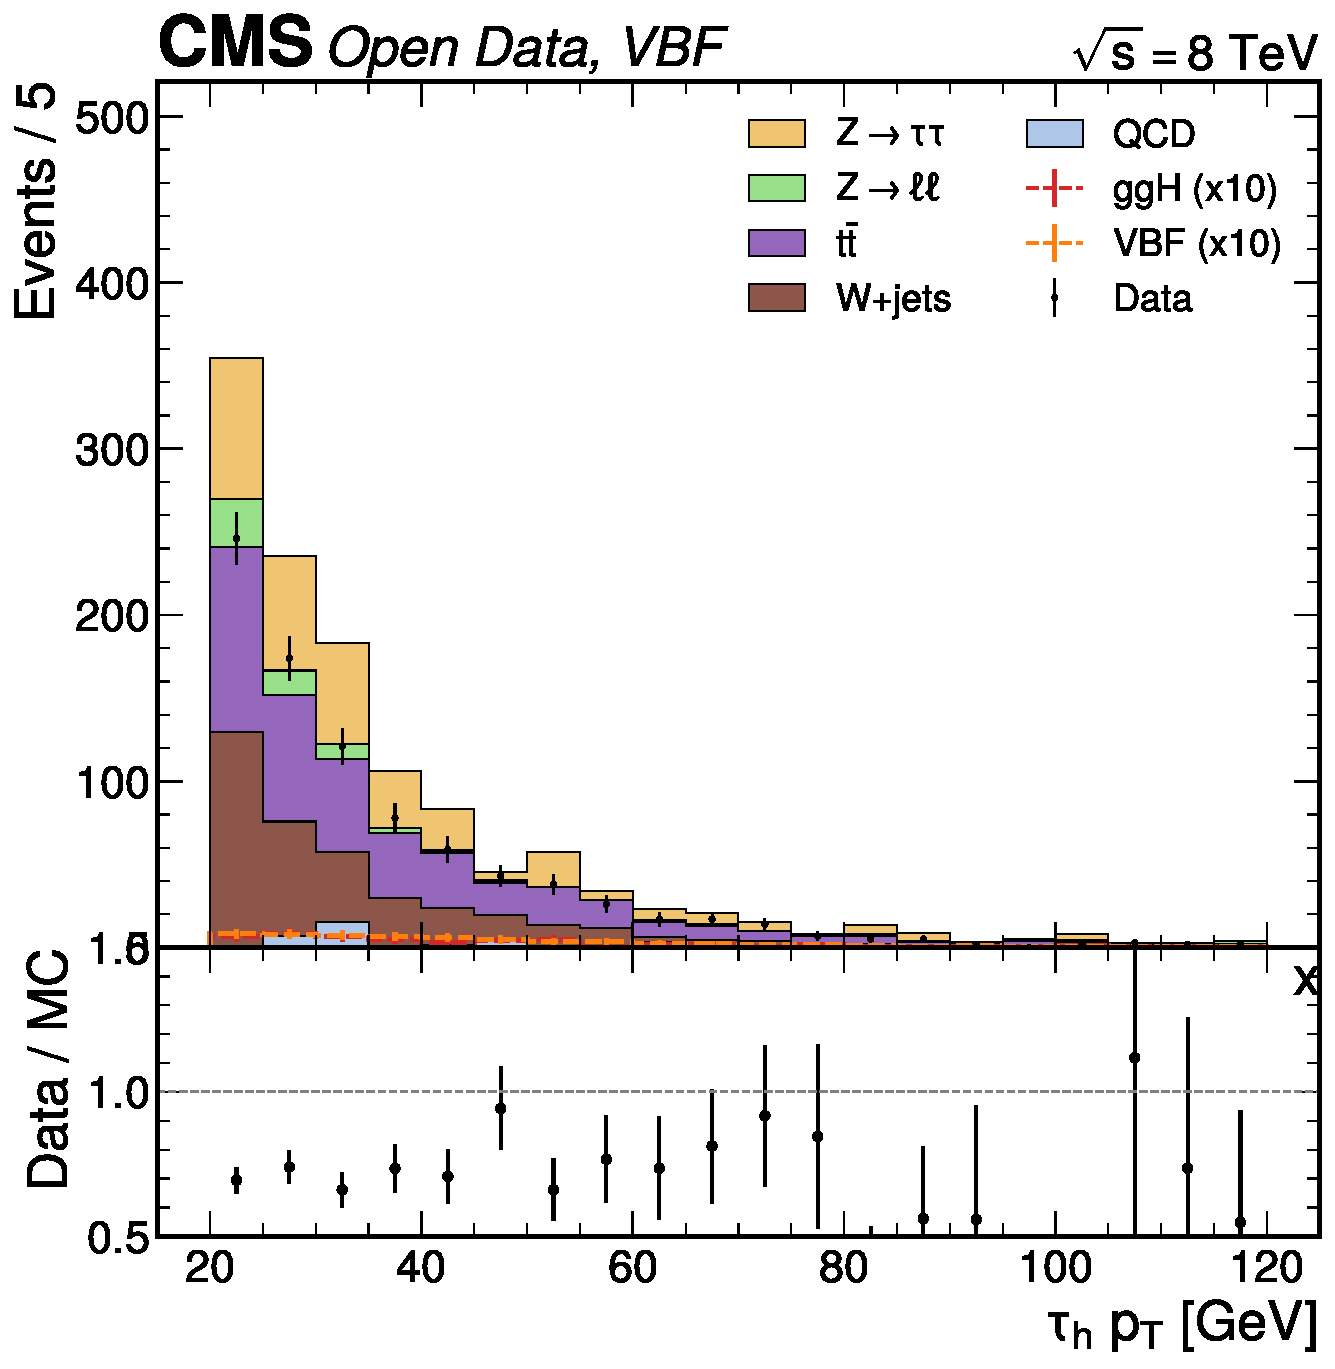
\includegraphics[height=0.38\linewidth,keepaspectratio]{figures/tau_pt_vbf.pdf}\hspace{0.02\linewidth}
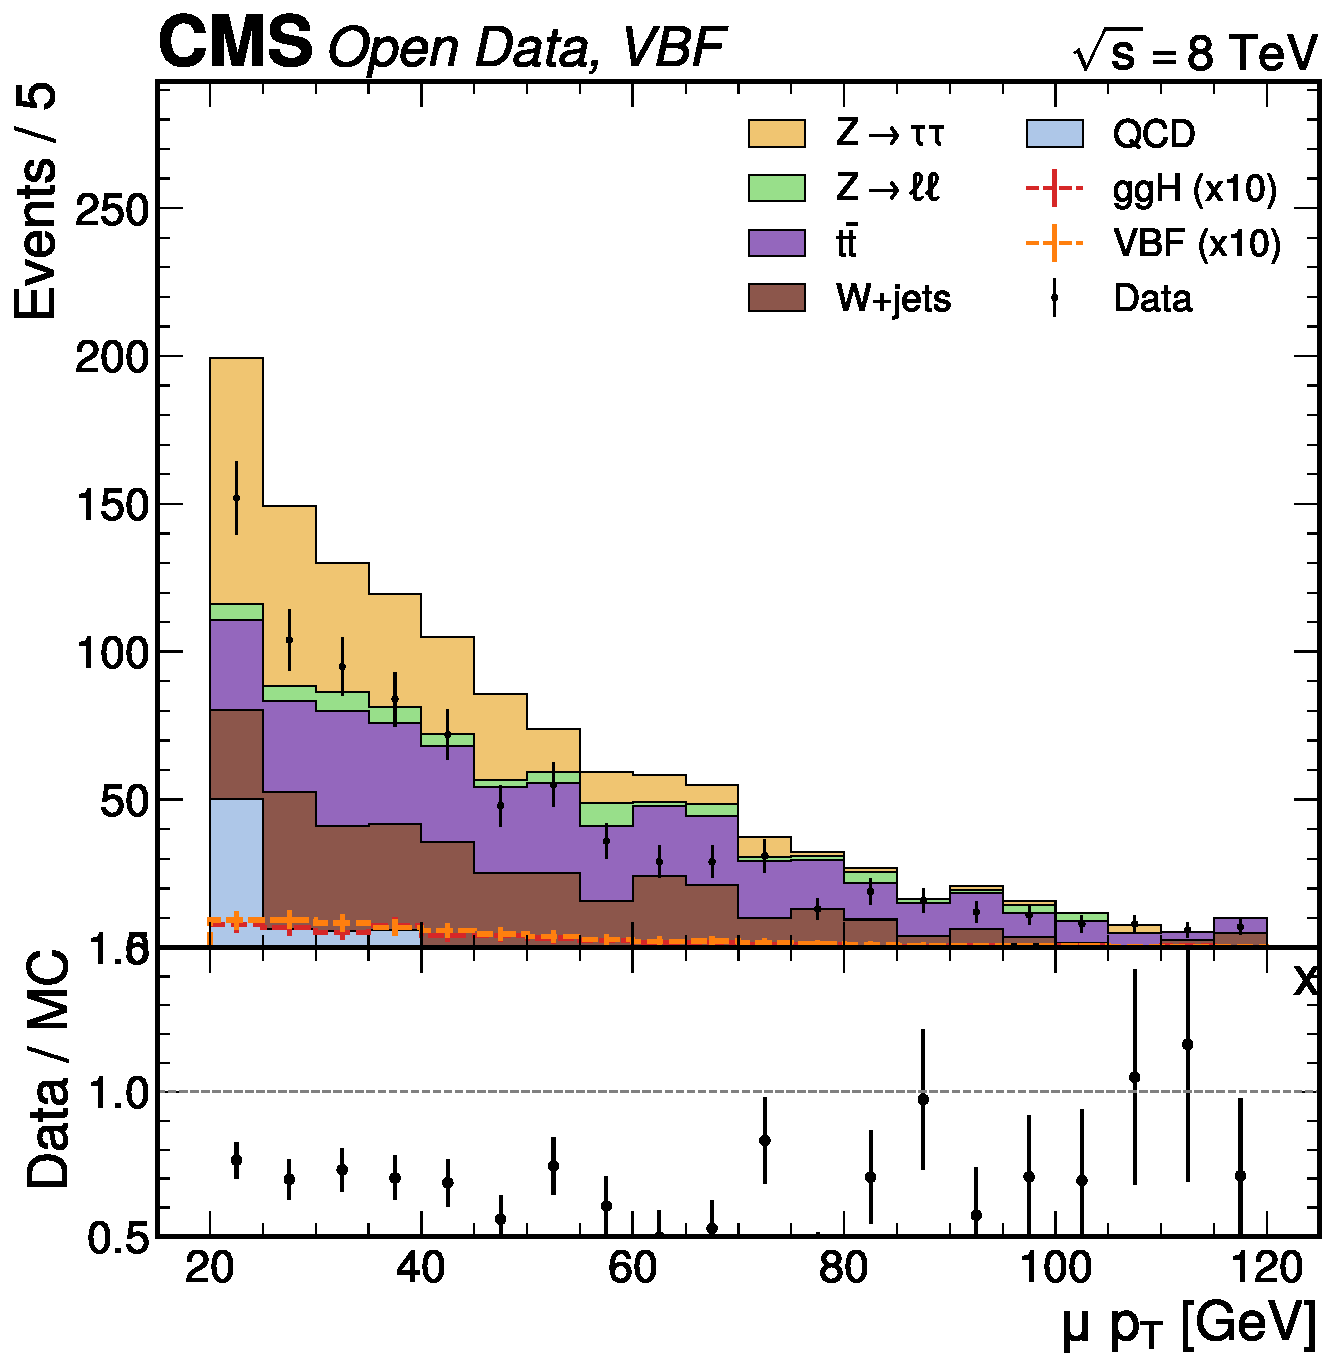
\includegraphics[height=0.38\linewidth,keepaspectratio]{figures/mu_pt_vbf.pdf}
\caption{(a) Hadronic tau \(p_\mathrm{T}\) distribution in the VBF category.
The spectrum is harder than in the Baseline category due to the VBF
event topology, where the Higgs boson recoils against the forward jet
system. The reduced statistics lead to larger data/MC fluctuations in
the ratio panel. (b) Muon \(p_\mathrm{T}\) distribution in the VBF category. The VBF
signal events (visible at the x10 scale) tend to have slightly harder
muon \(p_\mathrm{T}\) compared to the Baseline category, reflecting the
boost from the VBF production mechanism.}\label{fig:tau-pt-vbf}
\phantomsection\label{fig:mu-pt-vbf}
\end{figure}


\needspace{0.4\textheight}
\begin{figure}[htbp]
\centering
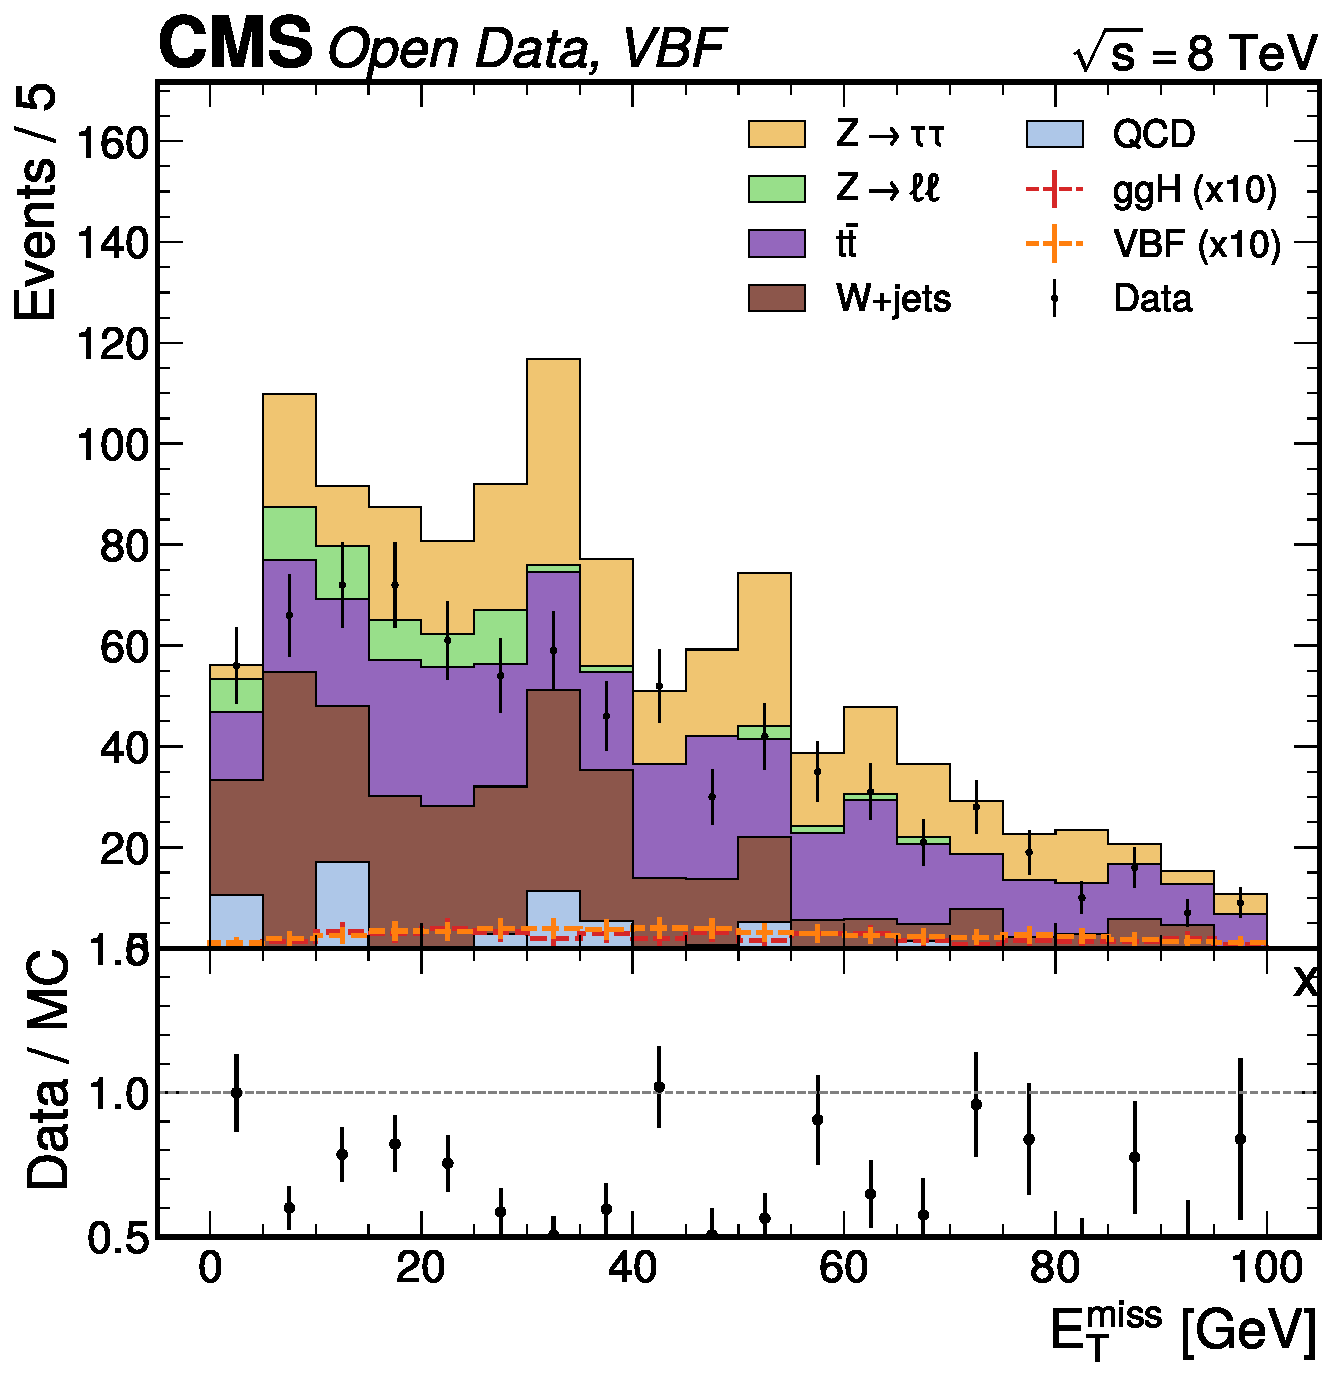
\includegraphics[height=0.38\linewidth,keepaspectratio]{figures/met_pt_vbf.pdf}\hspace{0.02\linewidth}
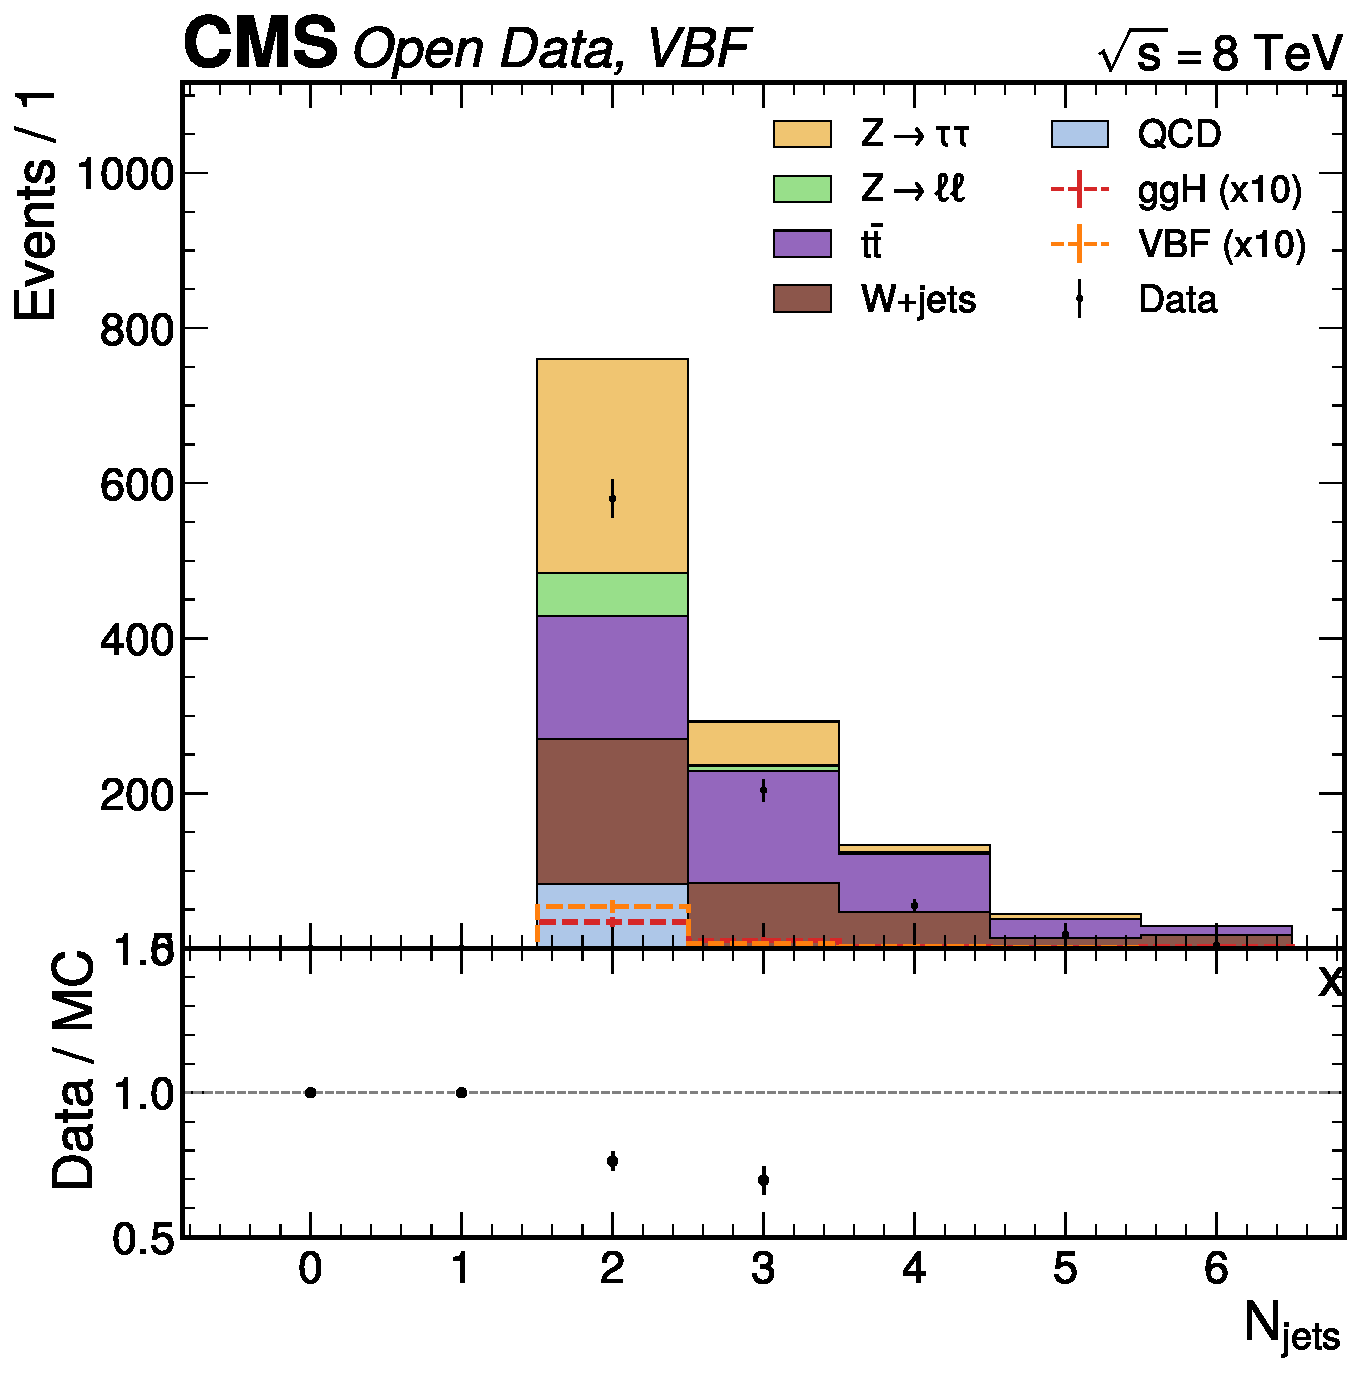
\includegraphics[height=0.38\linewidth,keepaspectratio]{figures/njets_vbf.pdf}
\caption{(a) Missing transverse energy distribution in the VBF category. The
\(t\bar{t}\) background contributes a larger fraction in this category
compared to Baseline, due to the two-jet requirement that naturally
selects \(t\bar{t}\) events. The MET distribution is broader than in
Baseline, consistent with the more complex event
topology. (b) Jet multiplicity distribution in the VBF category. By
construction, all events have at least two jets. The distribution shows
moderate agreement between data and MC, with the characteristic LO
generator jet multiplicity mismodeling less pronounced since the VBF
selection already requires two jets.}\label{fig:met-vbf}
\phantomsection\label{fig:njets-vbf}
\end{figure}


\needspace{0.4\textheight}
\begin{figure}[htbp]
\centering
\pandocbounded{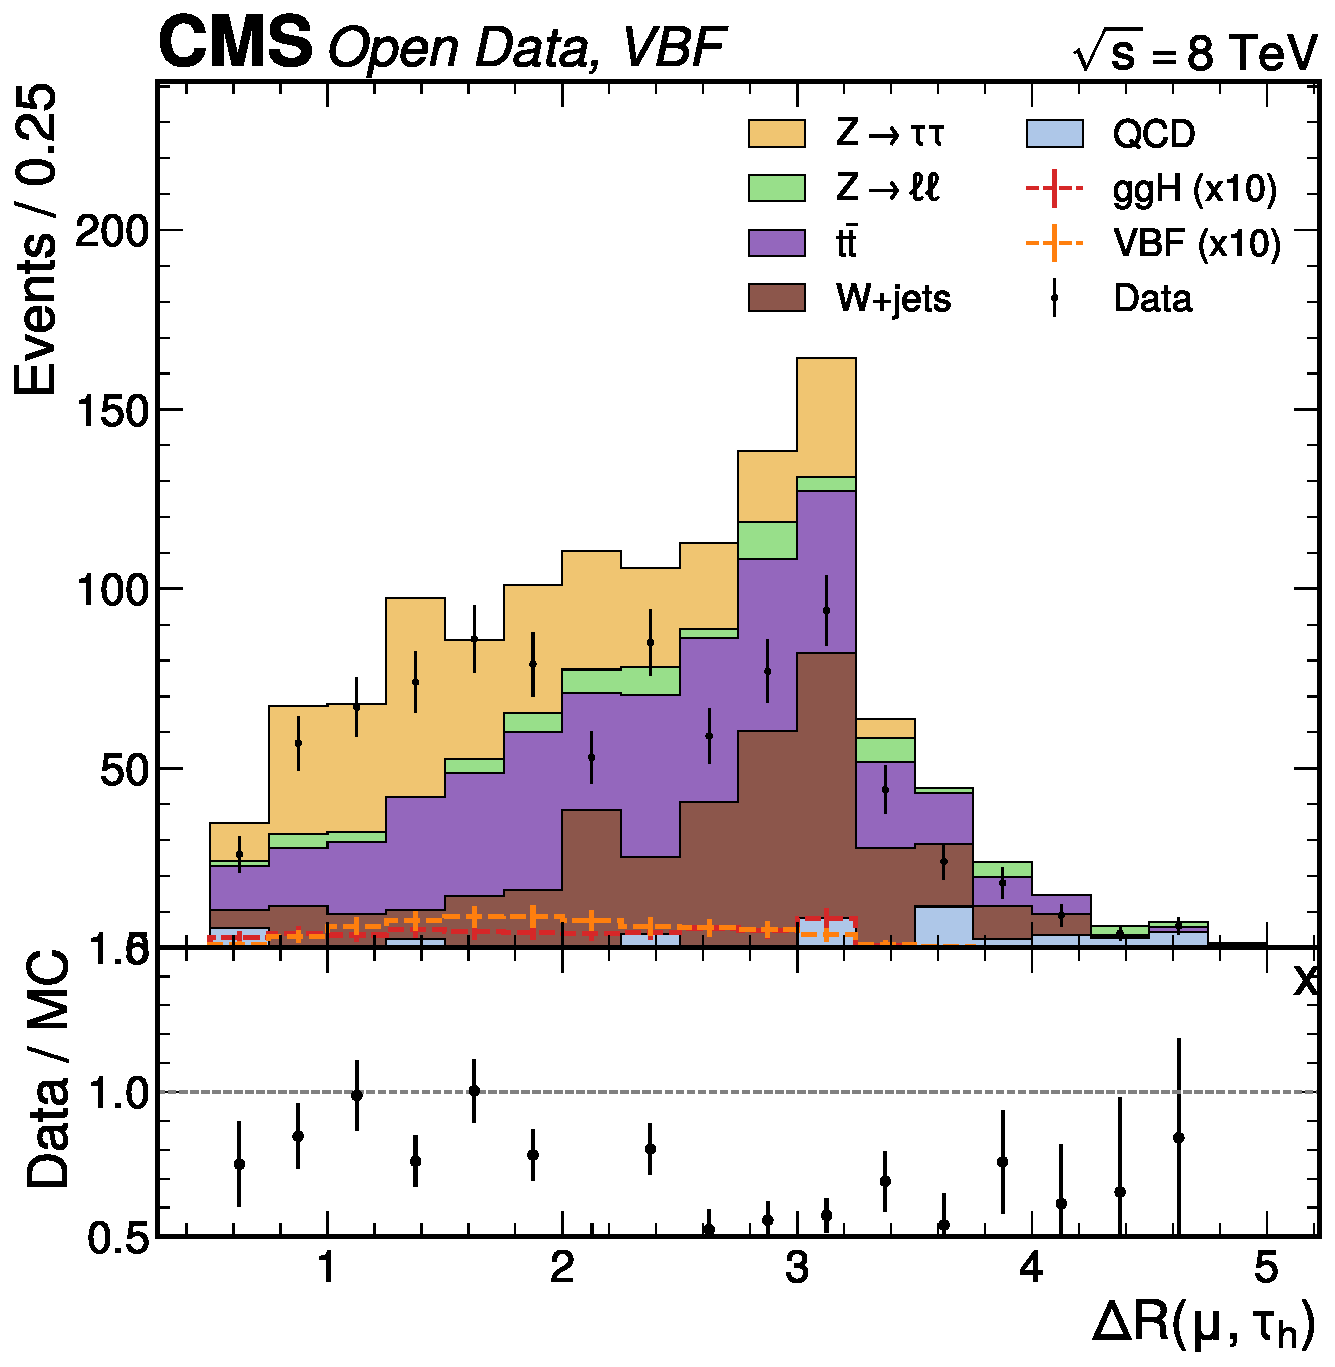
\includegraphics[height=0.35\textheight,width=\linewidth,keepaspectratio,alt={Angular separation \textbackslash Delta R(\textbackslash mu, \textbackslash tau\_\textbackslash mathrm\{h\}) in the VBF category. The distribution is slightly more forward-peaked than in the Baseline category, consistent with the more boosted kinematics of VBF events where the Higgs boson recoils against the dijet system.}]{figures/delta_r_vbf.pdf}}
\caption{Angular separation \(\Delta R(\mu, \tau_\mathrm{h})\) in the
VBF category. The distribution is slightly more forward-peaked than in
the Baseline category, consistent with the more boosted kinematics of
VBF events where the Higgs boson recoils against the dijet
system.}\label{fig:delta-r-vbf}
\end{figure}

\needspace{4\baselineskip}
\subsection{Variable separation power}\label{sec:var-separation}

\needspace{0.4\textheight}
\begin{figure}[htbp]
\centering
\pandocbounded{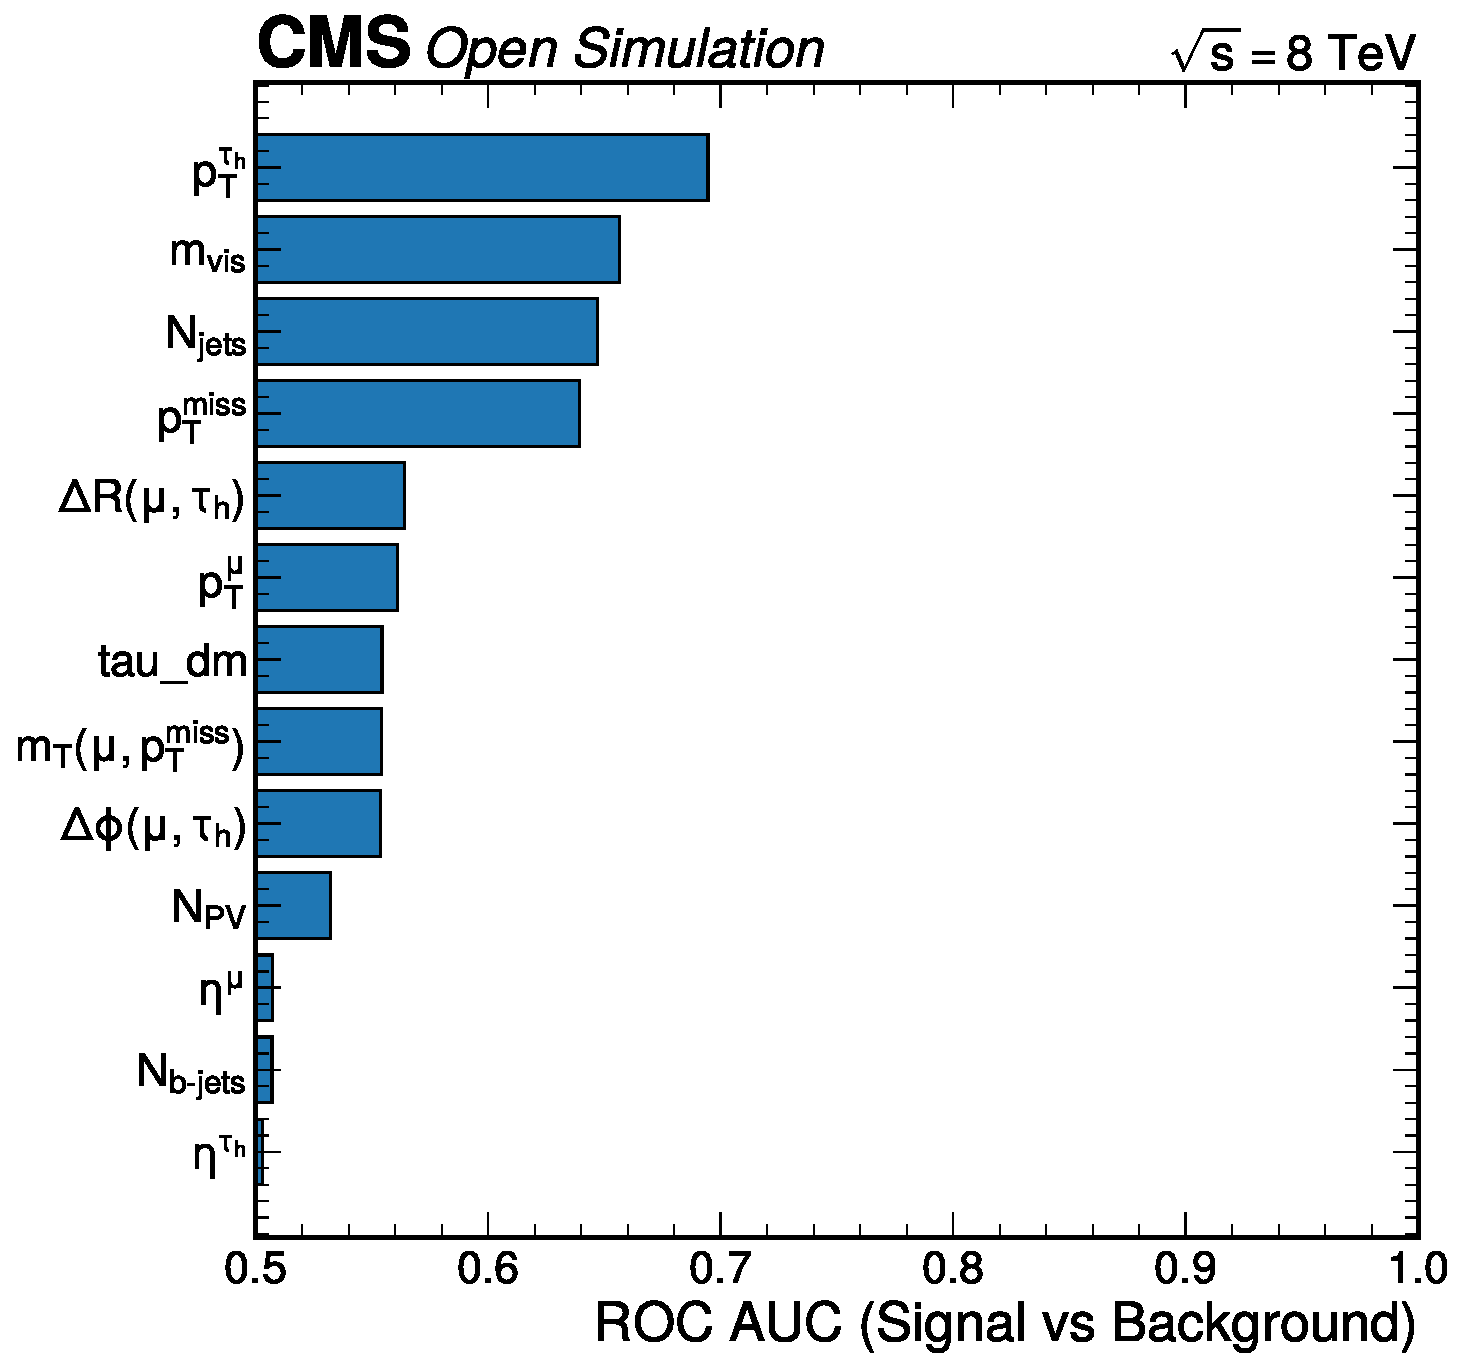
\includegraphics[height=0.35\textheight,width=\linewidth,keepaspectratio,alt={Ranking of kinematic variables by their individual signal-vs-background separation power, quantified by the ROC AUC. The top variables (\textbackslash tau\_\textbackslash mathrm\{h\} p\_\textbackslash mathrm\{T\}, m\_\textbackslash mathrm\{vis\}, N\_\textbackslash mathrm\{jets\}, E\_\textbackslash mathrm\{T\}\^{}\textbackslash mathrm\{miss\}) all have AUC \textgreater{} 0.63, while pseudorapidity variables show minimal discrimination (AUC near 0.5). The NN combines all 14 variables to achieve a test AUC of 0.825.}]{figures/separation_power.pdf}}
\caption{Ranking of kinematic variables by their individual
signal-vs-background separation power, quantified by the ROC AUC. The
top variables (\(\tau_\mathrm{h}\) \(p_\mathrm{T}\), \(m_\mathrm{vis}\),
\(N_\mathrm{jets}\), \(E_\mathrm{T}^\mathrm{miss}\)) all have AUC
\textgreater{} 0.63, while pseudorapidity variables show minimal
discrimination (AUC near 0.5). The NN combines all 14 variables to
achieve a test AUC of 0.825.}\label{fig:separation-power}
\end{figure}

\needspace{4\baselineskip}
\FloatBarrier
\section{Statistical Method}\label{sec:statmethod}

\needspace{4\baselineskip}
\subsection{Profile likelihood framework}\label{sec:stat-likelihood}

The signal strength modifier \(\mu\) is extracted using a binned profile
likelihood ratio method implemented in pyhf
(\citeproc{ref-pyhf}{Heinrich et al. 2021};
\citeproc{ref-Cranmer:2012sba}{Cranmer et al. 2012}). For each fitting
approach (visible mass, NN discriminant, collinear mass), a simultaneous
fit is performed across the Baseline and VBF categories with a single
parameter of interest (POI):
\(\mu = \sigma_\mathrm{obs} / \sigma_\mathrm{SM}\).

The likelihood function is:

\begin{equation}\protect\phantomsection\label{eq:likelihood}{\mathcal{L}(\mu, \boldsymbol{\theta}) = \prod_{c \in \{\mathrm{Baseline, VBF}\}} \prod_{b=1}^{N_\mathrm{bins}} \mathrm{Pois}\left(n_{cb} \,\middle|\, \nu_{cb}(\mu, \boldsymbol{\theta})\right) \times \prod_{k=1}^{N_\mathrm{NP}} f_k(\theta_k)}\end{equation}

where \(n_{cb}\) is the observed count in bin \(b\) of category \(c\),
\(\nu_{cb}(\mu, \boldsymbol{\theta})\) is the expected count
parameterized by the signal strength \(\mu\) and nuisance parameters
\(\boldsymbol{\theta}\), and \(f_k(\theta_k)\) are constraint terms for
the nuisance parameters.

The expected yield in each bin is:

\begin{equation}\protect\phantomsection\label{eq:expected-yield}{\nu_{cb}(\mu, \boldsymbol{\theta}) = \mu \cdot s_{cb}(\boldsymbol{\theta}) + b_{cb}(\boldsymbol{\theta})}\end{equation}

where \(s_{cb}\) is the signal template (ggH + VBF, sharing a common
\(\mu\)) and \(b_{cb}\) is the total background template
(\(Z\to\tau\tau + Z\to\ell\ell + t\bar{t} + W\mathrm{+jets} + \mathrm{QCD}\)).
Both signal and background templates are functions of the nuisance
parameters \(\boldsymbol{\theta}\).

The test statistic used for limit setting and significance is the
profile likelihood ratio:

\begin{equation}\protect\phantomsection\label{eq:test-statistic}{q_\mu = -2 \ln \frac{\mathcal{L}(\mu, \hat{\hat{\boldsymbol{\theta}}})}{\mathcal{L}(\hat{\mu}, \hat{\boldsymbol{\theta}})}}\end{equation}

where \(\hat{\mu}\) and \(\hat{\boldsymbol{\theta}}\) are the
unconditional maximum likelihood estimates, and
\(\hat{\hat{\boldsymbol{\theta}}}\) are the conditional maximum
likelihood estimates of \(\boldsymbol{\theta}\) for a given \(\mu\)
(\citeproc{ref-Cowan:2010js}{Cowan et al. 2011}).

\needspace{4\baselineskip}
\subsection{Nuisance parameter treatment}\label{sec:stat-nps}

The model includes 21 nuisance parameters encoding systematic
uncertainties, plus Barlow-Beeston lite statistical uncertainty
parameters (one per bin per channel)
(\citeproc{ref-Barlow:1993dm}{Barlow and Beeston 1993}). The total
number of parameters per workspace is approximately 71 (21 NPs + 50
staterror gammas + 1 POI).

Normalization systematics (normsys) modify the overall yield of affected
processes by a multiplicative factor \(\kappa^{\theta_k}\), where
\(\theta_k\) is a unit-Gaussian nuisance parameter. Shape systematics
(histosys) interpolate between up/down template variations using
piecewise-linear interpolation.

\needspace{4\baselineskip}
\subsection{CLs method for upper limits}\label{sec:stat-cls}

The expected 95\% confidence level (CL) upper limit on \(\mu\) is
computed using the CL\(_\mathrm{s}\) method
(\citeproc{ref-Read:2002hq}{Read 2002}) with the \(\tilde{q}_\mu\) test
statistic. The CL\(_\mathrm{s}\) value is:

\begin{equation}\protect\phantomsection\label{eq:cls}{\mathrm{CL}_\mathrm{s}(\mu) = \frac{p_{s+b}(\mu)}{1 - p_b(\mu)}}\end{equation}

where \(p_{s+b}\) is the \(p\)-value under the signal-plus-background
hypothesis and \(p_b\) is the \(p\)-value under the background-only
hypothesis. The 95\% CL upper limit is the value of \(\mu\) for which
CL\(_\mathrm{s} = 0.05\). The \(p\)-values are computed using asymptotic
formulae (\citeproc{ref-Cowan:2010js}{Cowan et al. 2011}).

\needspace{4\baselineskip}
\FloatBarrier
\section{Systematic Uncertainties}\label{sec:systematics}

This section describes each source of systematic uncertainty included in
the statistical model. Each systematic is characterized by its physical
origin, evaluation method, numerical impact on the signal strength
\(\mu\), and interpretation. The systematic sources are categorized as
normalization uncertainties (affecting the overall yield) and shape
uncertainties (affecting the template shape). A summary table is
provided in Table~\ref{tbl:syst-summary} and the impact ranking is
presented in Section~\ref{sec:syst-ranking}.

\needspace{4\baselineskip}
\subsection{Luminosity}\label{sec:syst-lumi}

The integrated luminosity measurement for the 2012 CMS data has an
uncertainty of 2.6\%, as determined by the CMS luminosity group using
pixel cluster counting (\citeproc{ref-CMS:LUM-13-001}{CMS Collaboration
2013}). This uncertainty is applied as a fully correlated normalization
systematic on all MC-predicted processes (signal and backgrounds). The
QCD multijet background, which is estimated from data, is not affected.
The impact on \(\mu\) is \(\pm 0.069\), ranking 6th among all nuisance
parameters. This is expected: the luminosity uncertainty scales all MC
predictions simultaneously, and its impact on \(\mu\) is modulated by
the signal-to-background ratio.

\needspace{4\baselineskip}
\subsection{\texorpdfstring{\(Z\to\tau\tau\)
normalization}{Z\textbackslash to\textbackslash tau\textbackslash tau normalization}}\label{sec:syst-znorm}

The \(Z\to\tau\tau\) and \(Z\to\ell\ell\) background normalizations
carry a 12\% uncertainty, applied as a correlated normalization
systematic. This uncertainty is decomposed as the quadrature sum of five
components: theory cross-section (4\%, from the FEWZ NNLO calculation),
trigger efficiency data/MC difference (5\%, due to the absence of
trigger scale factors for CMS Open Data), tau identification loosening
effect (8\%, from the enlarged phase space at the Loose working point
without official scale factors), statistical precision in the \(Z\) peak
validation region (2\%), and a 5\% additional margin for residual pileup
mismodeling and other unaccounted effects. The quadrature sum is
\(\sqrt{4^2 + 5^2 + 8^2 + 2^2 + 5^2} = \sqrt{134} \approx 11.6\%\),
rounded to 12\%. The trigger efficiency component is absorbed into this
normalization rather than being treated as a separate systematic for DY,
to avoid double-counting. Published analyses using tau-embedded
\(Z\to\mu\mu\) data samples achieve Z normalization uncertainties of
3-4\% (\citeproc{ref-CMS:2014nkk}{{Chatrchyan et al.} 2014};
\citeproc{ref-CMS:2017zyp}{{Sirunyan et al.} 2018a}); the larger
uncertainty here reflects the CMS Open Data constraints. The impact on
\(\mu\) is \(\pm 0.036\), ranking 14th, because the \(Z\to\tau\tau\)
background contributes primarily in the low-NN-score region where signal
is absent.

\needspace{4\baselineskip}
\subsection{\texorpdfstring{\(t\bar{t}\)
normalization}{t\textbackslash bar\{t\} normalization}}\label{sec:syst-ttbar}

The \(t\bar{t}\) background normalization carries a 5\% uncertainty
based on the NNLO+NNLL cross-section calculation using Top++ v2.0
(\citeproc{ref-Czakon:2011xx}{Czakon and Mitov 2014}) at \(m_t = 172.5\)
GeV. The cross-section value of 252.9 pb has scale uncertainties of
+6.4/-8.6 pb and PDF+\(\alpha_s\) uncertainties of ±7.8 pb, which
combine to approximately 5\% total. The impact on \(\mu\) is ±0.042,
ranking 12th. The \(t\bar{t}\) background contributes approximately 4\%
of the total background in the signal region and is more significant in
the VBF category (where it constitutes approximately 35\% of the
background due to the two-jet requirement).

\needspace{4\baselineskip}
\subsection{\texorpdfstring{\(W\)+jets
normalization}{W+jets normalization}}\label{sec:syst-wjets}

The \(W\)+jets background normalization carries a 10\% uncertainty per
category, treated as uncorrelated between the Baseline and VBF
categories. The data-driven scale factor
(\(\mathrm{SF}_W = 0.999 \pm 0.008\)) has a statistical uncertainty of
0.8\%, but the dominant uncertainty comes from the transverse mass
extrapolation from the high-\(m_\mathrm{T}\) sideband
(\(m_\mathrm{T} > 70\) GeV) to the signal region (\(m_\mathrm{T} < 30\)
GeV), estimated at approximately 10\% by comparing the \(W\)+jets shape
in the high-\(m_\mathrm{T}\) and intermediate-\(m_\mathrm{T}\) regions.
The impact on \(\mu\) is \(\pm 0.044\) in the Baseline category and
\(\pm 0.065\) in the VBF category (ranked 11th and 8th, respectively).
The larger VBF impact reflects the smaller total background count in
that category.

\needspace{4\baselineskip}
\subsection{QCD normalization}\label{sec:syst-qcd}

The QCD multijet background normalization carries a 20\% uncertainty per
category, treated as uncorrelated between categories. This uncertainty
encompasses the statistical uncertainty on the OS/SS ratio measurement
(\(R_\mathrm{OS/SS} = 0.979 \pm 0.018\), approximately 2\%), the
methodological uncertainty from the same-sign estimation procedure, and
the extrapolation from the anti-isolated measurement region to the
signal region isolation. The 20\% value is conservative but justified by
the 30\% spread between literature values for \(R_\mathrm{OS/SS}\)
(tutorial: 0.80, published: 1.06, this analysis: 0.98) and the
Data/Prediction deficit of 6\% observed after including the QCD
estimate. The impact on \(\mu\) is \(\pm 0.065\) in the Baseline
category (ranked 7th) and \(\pm 0.025\) in the VBF category. The
Baseline impact is larger because the QCD multijet background
constitutes approximately 15\% of the total background in that category.

\needspace{4\baselineskip}
\subsection{Signal cross-section theory
uncertainty}\label{sec:syst-signal-theory}

\subsubsection{ggH scale variations}\label{ggh-scale-variations}

The ggH production cross-section has asymmetric scale uncertainties of
\(+4.4\%/-6.9\%\) from \(\mu_R/\mu_F\) variations, as computed at N3LO
QCD by the LHC Higgs Cross Section Working Group
(\citeproc{ref-LHCHiggsCrossSectionWorkingGroup:2016ypw}{{Florian et
al.} 2017}). This is implemented as an asymmetric normalization
systematic on the ggH signal. The impact on \(\mu\) is +0.048/-0.017
(ranked 15th), reflecting the small signal fraction relative to the
total expected yield.

\subsubsection{VBF scale variations}\label{vbf-scale-variations}

The VBF production cross-section has scale uncertainties of
\(+0.3\%/-0.2\%\) at NNLO QCD + NLO EW
(\citeproc{ref-LHCHiggsCrossSectionWorkingGroup:2016ypw}{{Florian et
al.} 2017}). The impact on \(\mu\) is negligible (\(\pm 0.0002\)), as
the VBF cross-section uncertainty is an order of magnitude smaller than
ggH and the VBF signal is a small fraction of the total signal yield.

\subsubsection{\texorpdfstring{PDF and \(\alpha_s\)
uncertainties}{PDF and \textbackslash alpha\_s uncertainties}}\label{pdf-and-alpha_s-uncertainties}

The ggH and VBF production cross-sections have PDF+\(\alpha_s\)
uncertainties of 3.2\% and 2.2\%, respectively
(\citeproc{ref-LHCHiggsCrossSectionWorkingGroup:2016ypw}{{Florian et
al.} 2017}). These are implemented as normalization-only systematics
(one for each production mode). The reduced NanoAOD format does not
contain LHEPdfWeight branches for event-level PDF reweighting, so the
acceptance effects of PDF variations (typically \textless{} 1-2\% for
\(H\to\tau\tau\) selection) are not covered. This limitation is common
in CMS Open Data analyses. The impact on \(\mu\) is \(\pm 0.013\) for
ggH PDF and \(\pm 0.003\) for VBF PDF.

\subsubsection{Branching ratio
uncertainty}\label{branching-ratio-uncertainty}

The \(H\to\tau\tau\) branching ratio has a combined uncertainty of 1.7\%
from parametric (quark mass, \(\alpha_s\)) and theoretical higher-order
uncertainties
(\citeproc{ref-LHCHiggsCrossSectionWorkingGroup:2016ypw}{{Florian et
al.} 2017}). This is applied as a correlated normalization systematic on
both ggH and VBF signal. The impact on \(\mu\) is \(\pm 0.007\), which
is small because the branching ratio uncertainty equally scales the
signal yield and does not affect the signal shape.

\needspace{4\baselineskip}
\subsection{Trigger efficiency}\label{sec:syst-trigger}

A 3\% trigger efficiency uncertainty is applied to signal, \(t\bar{t}\),
and \(W\)+jets processes. It is explicitly not applied to
\(Z\to\tau\tau\) and \(Z\to\ell\ell\), where the trigger efficiency
uncertainty is absorbed into the 12\% \(Z\) normalization uncertainty
(Section~\ref{sec:syst-znorm}) to avoid double-counting. The 3\%
value represents the residual trigger efficiency uncertainty after
accounting for the fact that the cross-trigger plateau region is well
above the offline \(p_\mathrm{T}\) thresholds (20 GeV offline vs 17 GeV
trigger for the muon leg). No trigger efficiency scale factors are
available for CMS Open Data. The impact on \(\mu\) is \(\pm 0.086\)
(ranked 5th), making trigger efficiency the leading normalization
systematic after the four shape systematics.

\needspace{4\baselineskip}
\subsection{Tau identification efficiency}\label{sec:syst-tauid}

A 5\% tau identification efficiency uncertainty is applied to processes
with genuine hadronic taus: signal (ggH and VBF) and \(Z\to\tau\tau\).
This value is adopted from the CMS tau performance group recommendation
for the Loose isolation working point, reduced from the 10\% placeholder
in the strategy because the Loose working point is well-studied and the
5\% value is consistent with published analyses
(\citeproc{ref-CMS:2014nkk}{{Chatrchyan et al.} 2014};
\citeproc{ref-CMS:2018jrd}{{Sirunyan et al.} 2018b}). The impact on
\(\mu\) is \(\pm 0.051\) (ranked 10th). The tau ID uncertainty affects
the signal normalization directly and is therefore a significant
contributor to the overall signal strength uncertainty.

\needspace{4\baselineskip}
\subsection{Muon identification and isolation}\label{sec:syst-muon-id}

A 2\% combined uncertainty on muon identification and isolation
efficiency is applied to all MC-predicted processes (except QCD, which
is data-driven). This covers the efficiency of the tight muon ID, the
\(p_\mathrm{T}\)- and \(\eta\)-dependent isolation requirements, and the
impact parameter selections. The value is consistent with CMS muon
performance group recommendations and published analyses
(\citeproc{ref-CMS:2014nkk}{{Chatrchyan et al.} 2014}). The impact on
\(\mu\) is \(\pm 0.051\) (ranked 9th).

\needspace{4\baselineskip}
\subsection{b-tagging efficiency}\label{sec:syst-btag}

A 5\% b-tagging efficiency uncertainty is applied to the \(t\bar{t}\)
background, which relies on the CSV medium working point for b-jet
identification in validation studies. This uncertainty is taken from CMS
BTV POG recommendations and is consistent with the published b-tagging
efficiency measurements. The impact on \(\mu\) is \(\pm 0.042\) (ranked
13th), comparable to the \(t\bar{t}\) normalization uncertainty since
both affect the same process.

\needspace{4\baselineskip}
\subsection{Missing backgrounds}\label{sec:syst-missing}

A 5\% normalization uncertainty is applied to all MC-based backgrounds
(\(Z\to\tau\tau\), \(Z\to\ell\ell\), \(t\bar{t}\)) to account for
missing minor backgrounds (single top, diboson) that are not available
in the CMS Open Data sample set. The single top and diboson
contributions are estimated to account for 1-3\% of the total background
based on cross-section estimates (\citeproc{ref-CMS:2014nkk}{{Chatrchyan
et al.} 2014}), making the 5\% uncertainty conservative. This
uncertainty is not applied to data-driven backgrounds (\(W\)+jets, QCD).
The impact on \(\mu\) is \(\pm 0.032\) (ranked 16th).

\needspace{4\baselineskip}
\subsection{Tau energy scale}\label{sec:syst-tes}

The tau energy scale (TES) is the dominant shape systematic, with an
uncertainty of \(\pm 3\%\) applied to the hadronic tau \(p_\mathrm{T}\).
The variation is propagated to the MET by adjusting the MET components:

\begin{equation}\protect\phantomsection\label{eq:tes-met}{E_\mathrm{T,x}^{\mathrm{miss},\pm} = E_\mathrm{T,x}^\mathrm{miss} \mp \Delta p_{\mathrm{T},x}^\tau, \quad E_\mathrm{T,y}^{\mathrm{miss},\pm} = E_\mathrm{T,y}^\mathrm{miss} \mp \Delta p_{\mathrm{T},y}^\tau}\end{equation}

where
\(\Delta p_{\mathrm{T},x}^\tau = p_{\mathrm{T},x}^{\tau,\mathrm{varied}} - p_{\mathrm{T},x}^{\tau,\mathrm{nominal}}\).
The TES variation shifts all observables (\(m_\mathrm{vis}\),
\(m_\mathrm{col}\), NN score) through their dependence on the tau
\(p_\mathrm{T}\) and MET. For the NN score, all 15 input features are
recomputed with the varied tau \(p_\mathrm{T}\) and MET, and the trained
NN model is re-evaluated to produce shifted score templates.

The \(\pm 3\%\) TES uncertainty is the standard CMS tau performance
group value for 2012 data (\citeproc{ref-CMS:2018jrd}{{Sirunyan et al.}
2018b}), applied inclusively across tau decay modes. Published analyses
(\citeproc{ref-CMS:2014nkk}{{Chatrchyan et al.} 2014};
\citeproc{ref-CMS:2017zyp}{{Sirunyan et al.} 2018a}) use per-decay-mode
TES values (1-3\%); the inclusive 3\% is conservative. On Asimov data,
TES ranks 4th with a symmetric impact of 0.214 on \(\mu\). On the full
dataset, TES drops to 15th with a symmetric impact of only 0.025, due to
the strong data constraint on the TES nuisance parameter (post-fit
uncertainty 0.18, discussed in Section~\ref{sec:full-np-pulls}).
The full-data impact is shown in Figure~\ref{fig:syst-tes}.

\needspace{0.4\textheight}
\begin{figure}[htbp]
\centering
\pandocbounded{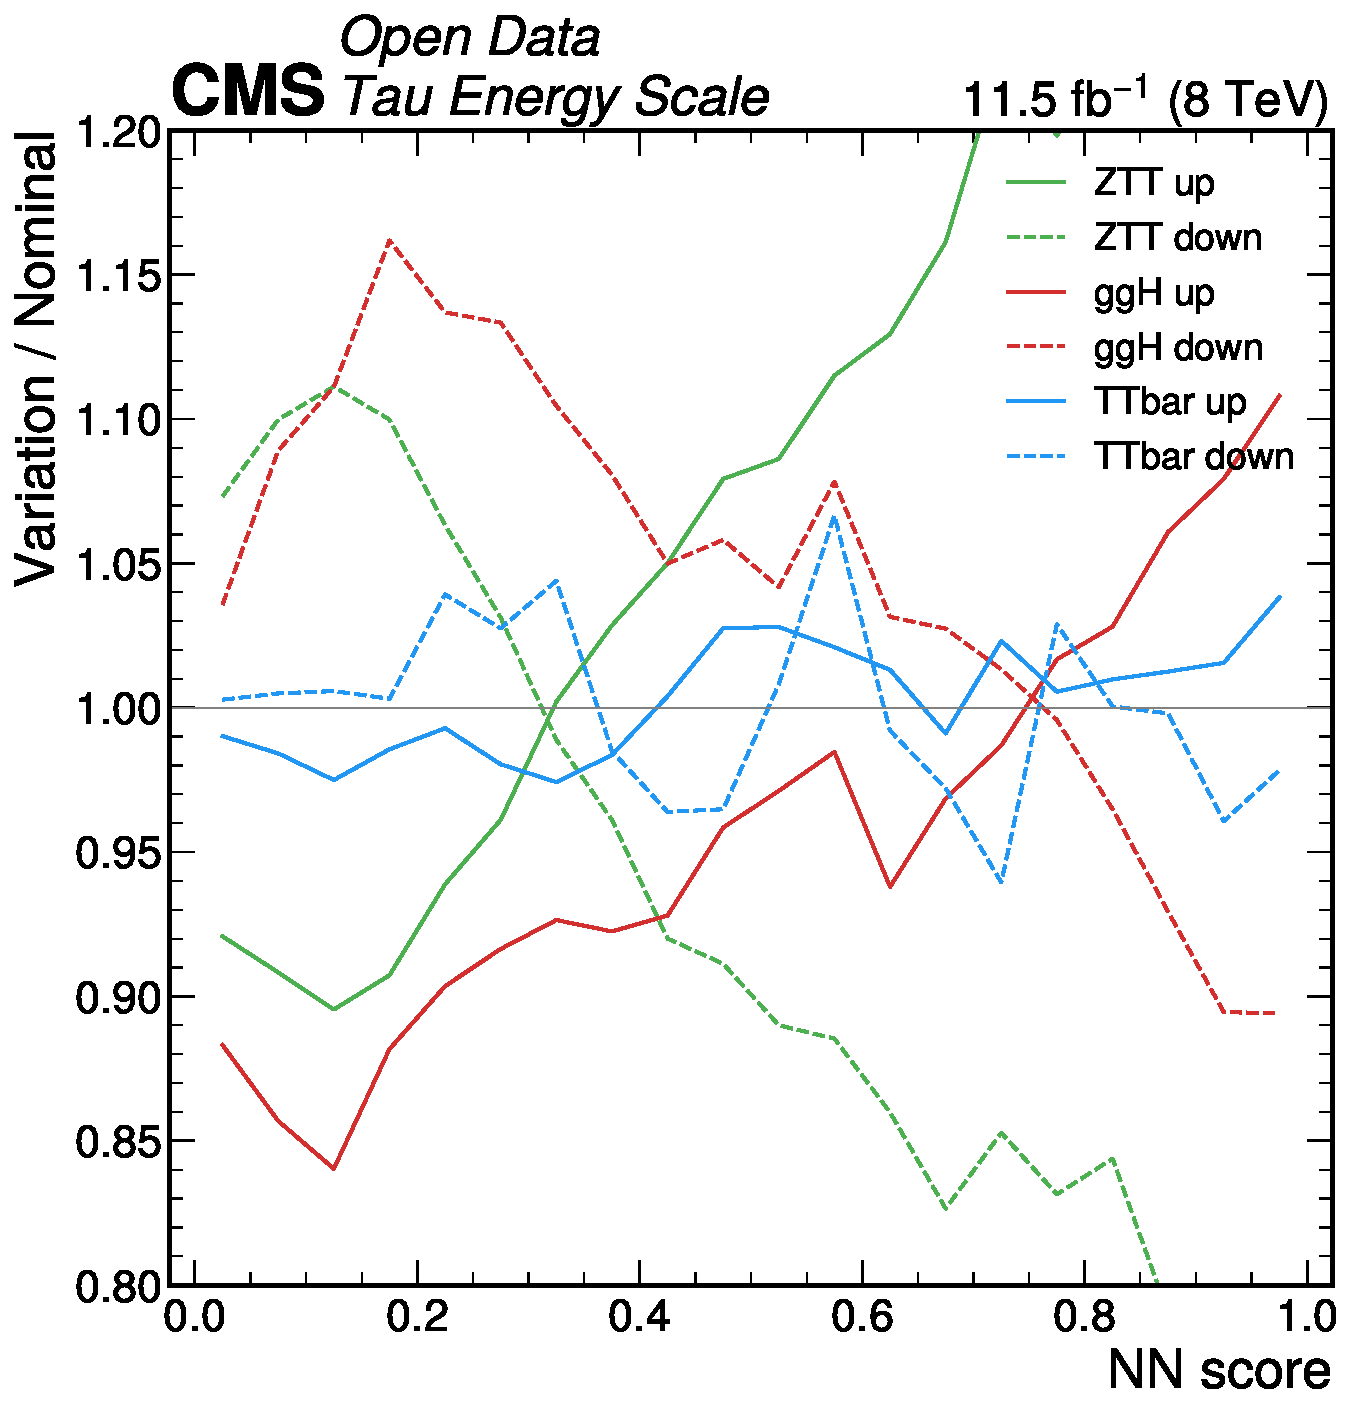
\includegraphics[height=0.35\textheight,width=\linewidth,keepaspectratio,alt={Ratio of the TES up (red) and down (blue) varied templates to the nominal template for Z\textbackslash to\textbackslash tau\textbackslash tau, ggH signal, and t\textbackslash bar\{t\} in the NN score Baseline channel. The TES variation produces bin-by-bin shape changes of order 5-20\%, with the largest effects in bins where the NN score distribution has steep gradients. The characteristic shape --- depletion in one region and enhancement in an adjacent region --- reflects the migration of events along the NN score axis as the tau energy is scaled.}]{figures/syst_shift_tes.pdf}}
\caption{Ratio of the TES up (red) and down (blue) varied templates to
the nominal template for \(Z\to\tau\tau\), ggH signal, and \(t\bar{t}\)
in the NN score Baseline channel. The TES variation produces bin-by-bin
shape changes of order 5-20\%, with the largest effects in bins where
the NN score distribution has steep gradients. The characteristic shape
--- depletion in one region and enhancement in an adjacent region ---
reflects the migration of events along the NN score axis as the tau
energy is scaled.}\label{fig:syst-tes}
\end{figure}

\needspace{4\baselineskip}
\subsection{Muon energy scale}\label{sec:syst-mes}

The muon energy scale (MES) uncertainty of \(\pm 1\%\) is applied to the
muon \(p_\mathrm{T}\), with analogous MET propagation to the TES. The
smaller variation magnitude (1\% vs 3\% for TES) reflects the better
muon momentum resolution compared to hadronic tau energy measurement. On
Asimov data, MES ranks 1st with a symmetric impact of 0.404 on \(\mu\).
On the full dataset, MES ranks 3rd with a symmetric impact of 0.148, as
shown in Figure~\ref{fig:syst-mes}. The MES is among the most
important systematics because the muon enters directly into the visible
mass, transverse mass, and MET calculations, affecting all observables.

\needspace{0.4\textheight}
\begin{figure}[htbp]
\centering
\pandocbounded{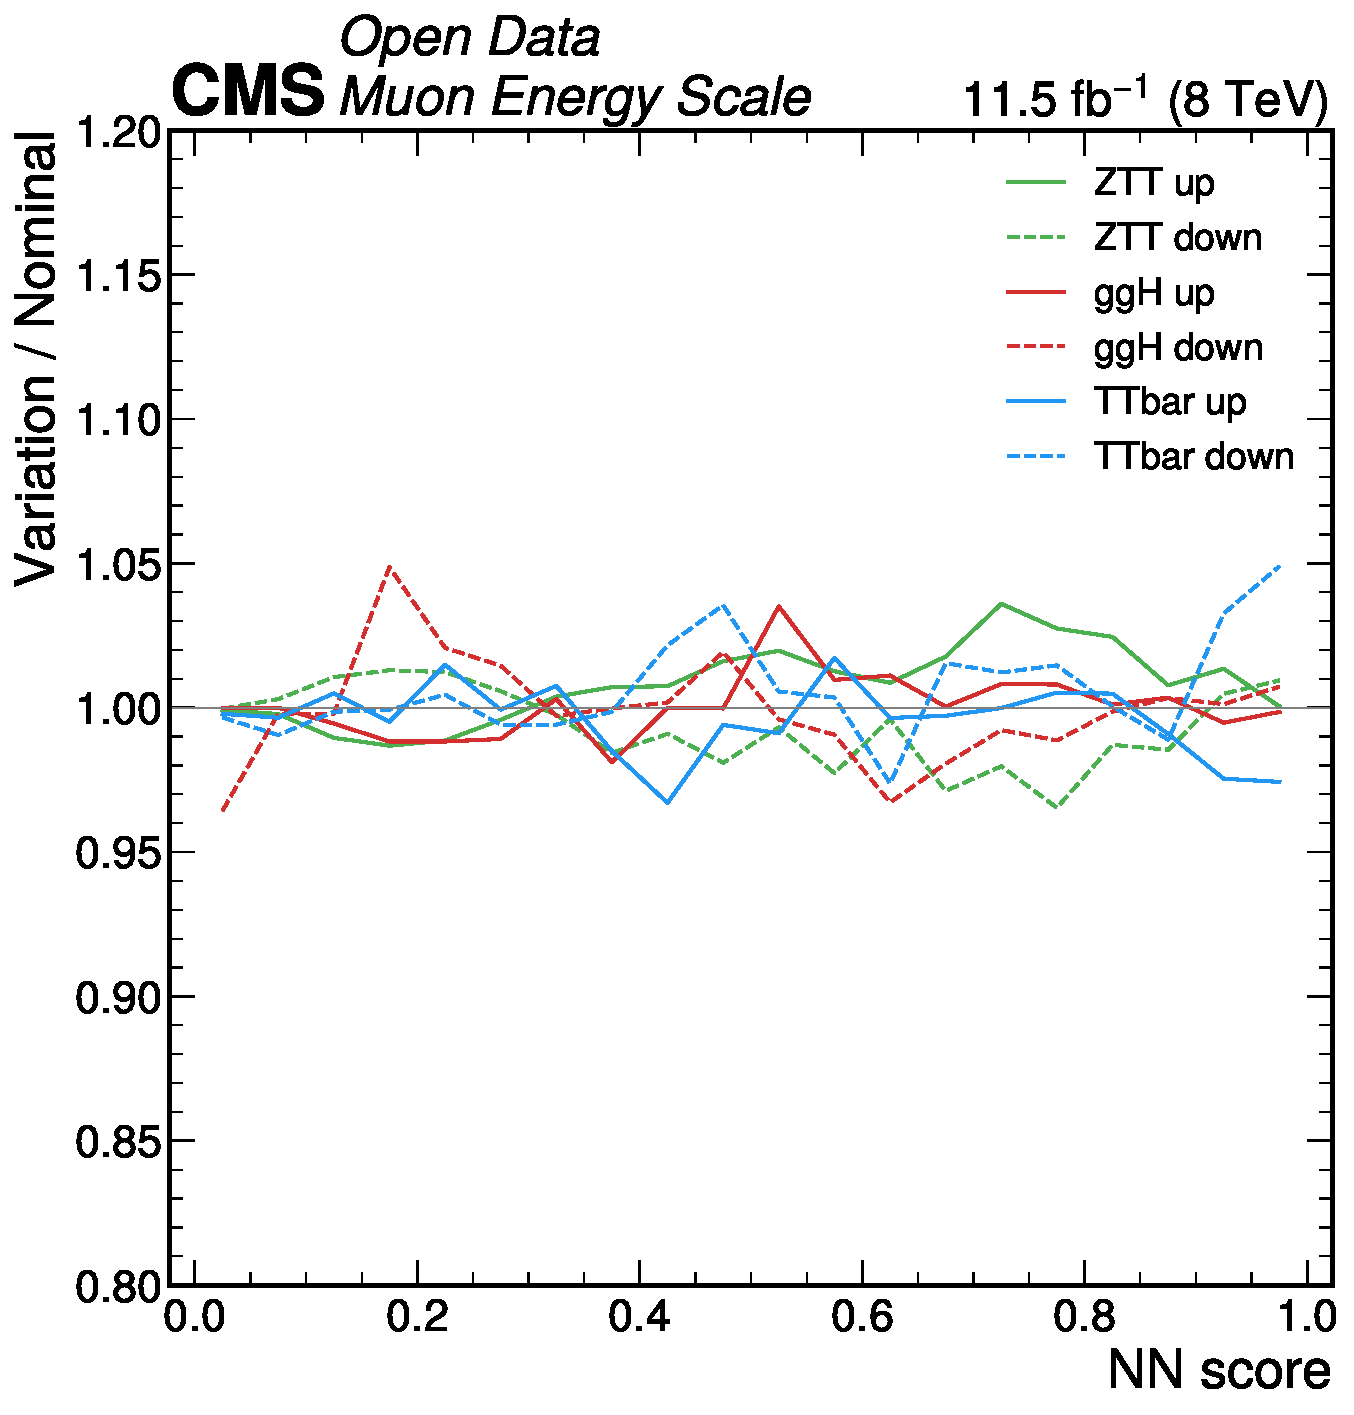
\includegraphics[height=0.35\textheight,width=\linewidth,keepaspectratio,alt={Ratio of the MES up and down varied templates to the nominal template for selected processes in the NN score Baseline channel. The 1\% MES variation produces smaller shape changes than the 3\% TES variation, but the impact on \textbackslash mu is still significant because the muon p\_\textbackslash mathrm\{T\} enters directly into the discriminant variable computation.}]{figures/syst_shift_mes.pdf}}
\caption{Ratio of the MES up and down varied templates to the nominal
template for selected processes in the NN score Baseline channel. The
1\% MES variation produces smaller shape changes than the 3\% TES
variation, but the impact on \(\mu\) is still significant because the
muon \(p_\mathrm{T}\) enters directly into the discriminant variable
computation.}\label{fig:syst-mes}
\end{figure}

\needspace{4\baselineskip}
\subsection{Jet energy scale}\label{sec:syst-jes}

The jet energy scale (JES) uncertainty of \(\pm 3\%\) is applied to all
jets, with propagation to the MET and re-evaluation of the VBF
categorization criteria (\(m_{jj}\), \(|\Delta\eta_{jj}|\)). The JES
variation causes events to migrate between the Baseline and VBF
categories as jets cross the 30 GeV \(p_\mathrm{T}\) threshold or the
VBF \(m_{jj}\) and \(|\Delta\eta_{jj}|\) thresholds shift. This category
migration is the key effect of JES, as it changes the relative event
composition between the two categories. The \(\pm 3\%\) value is
consistent with CMS jet energy correction uncertainties for 2012 data
(\citeproc{ref-CMS:2016lmd}{{Khachatryan et al.} 2017}). On Asimov data,
JES ranks 3rd with a symmetric impact of 0.267 on \(\mu\). On the full
dataset, JES ranks 2nd with a symmetric impact of 0.214 (Figure~\ref{fig:syst-jes}).

\needspace{0.4\textheight}
\begin{figure}[htbp]
\centering
\pandocbounded{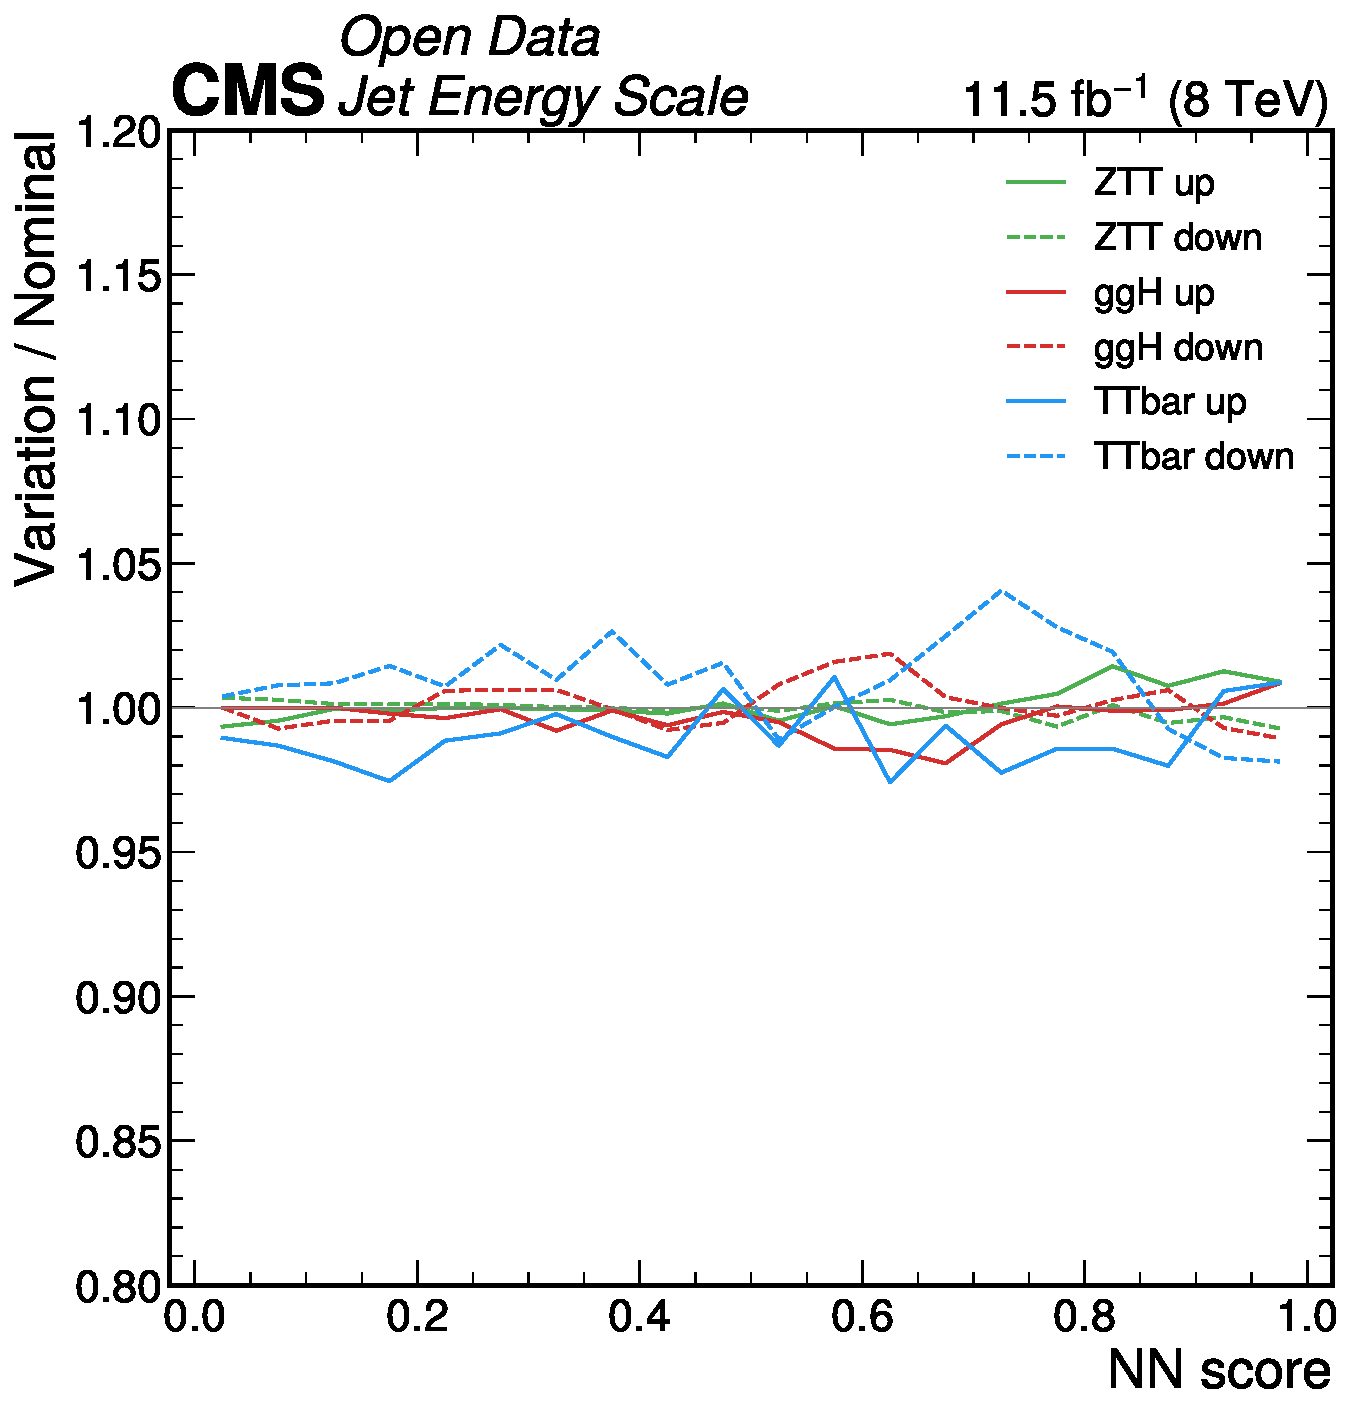
\includegraphics[height=0.35\textheight,width=\linewidth,keepaspectratio,alt={Ratio of the JES up and down varied templates to the nominal for selected processes in the NN score Baseline channel. The JES variation produces asymmetric effects due to category migration: JES up increases jet p\_\textbackslash mathrm\{T\} and moves more events into the VBF category, depleting the Baseline. The effect on the NN score distribution is less direct than TES/MES since jet p\_\textbackslash mathrm\{T\} enters the NN as a secondary input.}]{figures/syst_shift_jes.pdf}}
\caption{Ratio of the JES up and down varied templates to the nominal
for selected processes in the NN score Baseline channel. The JES
variation produces asymmetric effects due to category migration: JES up
increases jet \(p_\mathrm{T}\) and moves more events into the VBF
category, depleting the Baseline. The effect on the NN score
distribution is less direct than TES/MES since jet \(p_\mathrm{T}\)
enters the NN as a secondary input.}\label{fig:syst-jes}
\end{figure}

\needspace{4\baselineskip}
\subsection{MET unclustered energy}\label{sec:syst-met-uncl}

The unclustered energy contribution to the MET has an uncertainty of
\(\pm 10\%\), applied as a direct scaling of the MET magnitude.
Unclustered energy represents the soft hadronic activity not associated
with reconstructed jets, muons, or taus, and contributes significantly
to the MET resolution. The \(\pm 10\%\) variation is the standard CMS
recommendation for the unclustered energy uncertainty
(\citeproc{ref-CMS:PFT-09-001}{CMS Collaboration 2009}). On Asimov data,
MET unclustered ranks 2nd with a symmetric impact of 0.354 on \(\mu\).
On the full dataset, MET unclustered ranks 1st with a symmetric impact
of 0.285 (Figure~\ref{fig:syst-met-uncl}), making it the single
most important systematic uncertainty in the observed result. The impact
is driven by the MET entering the collinear mass calculation and NN
input features.

\needspace{0.4\textheight}
\begin{figure}[htbp]
\centering
\pandocbounded{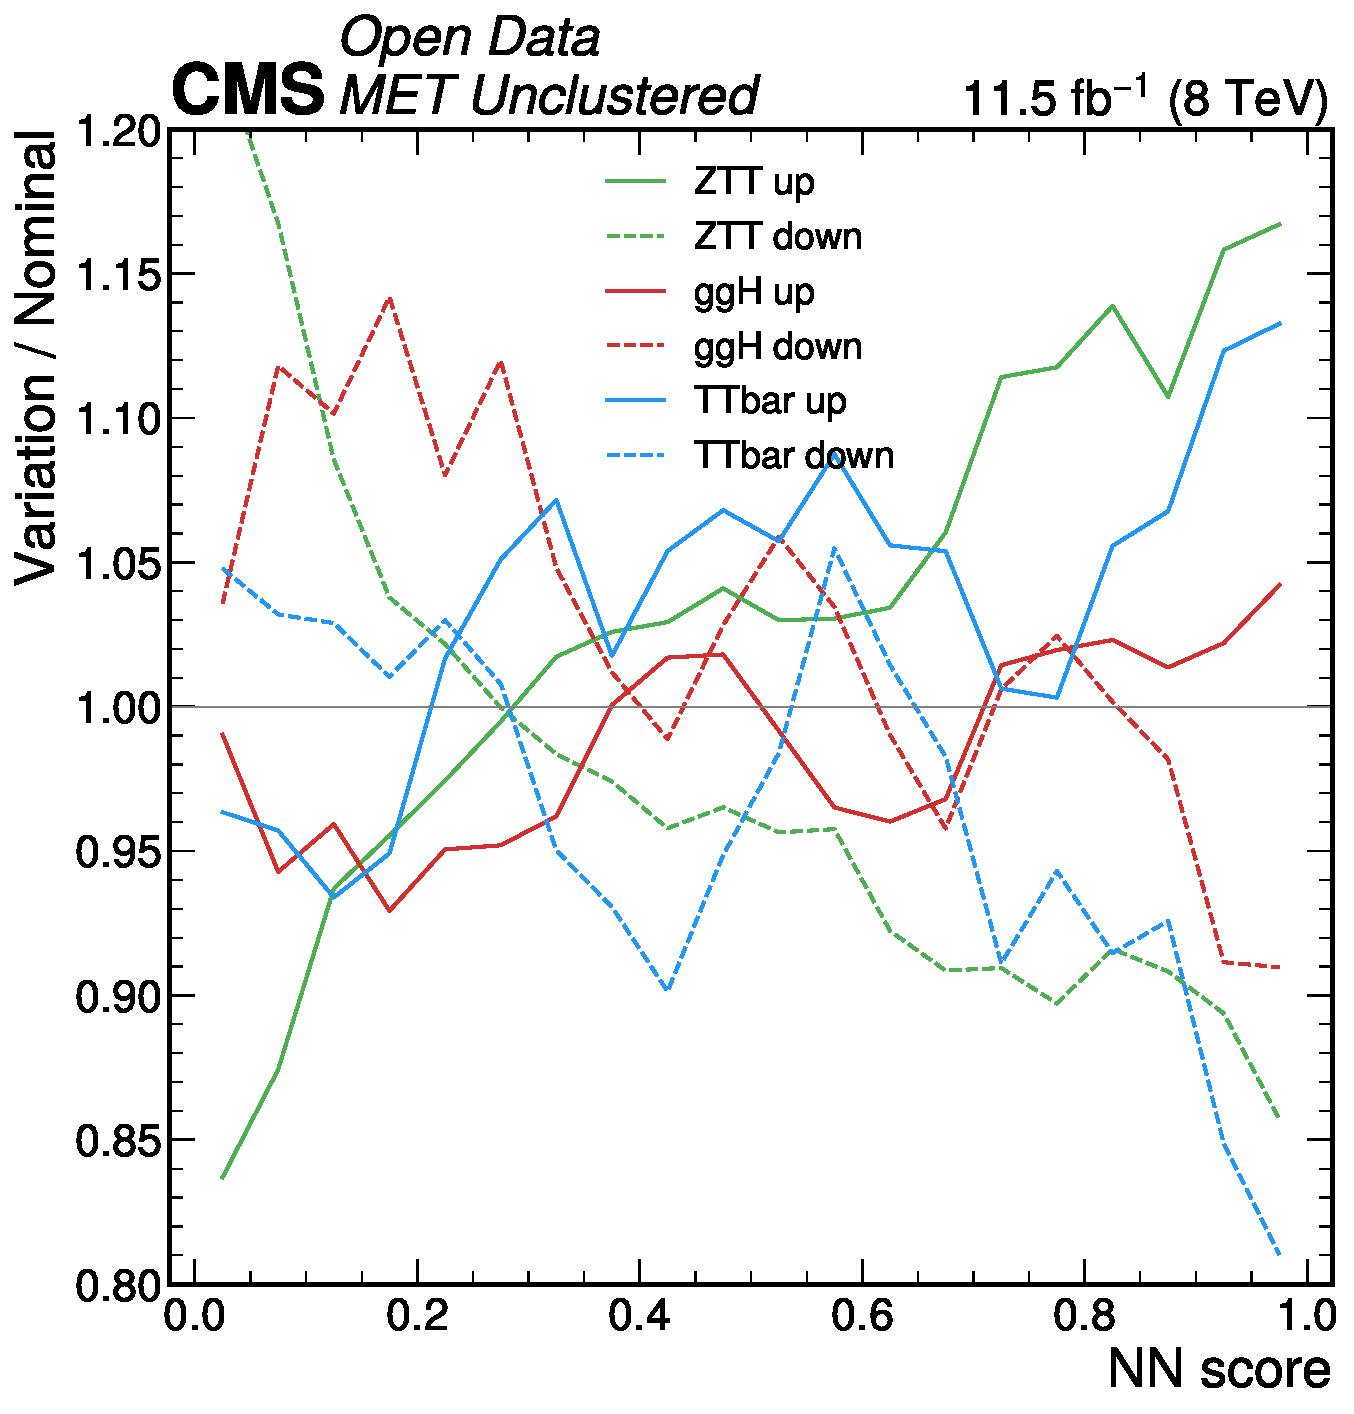
\includegraphics[height=0.35\textheight,width=\linewidth,keepaspectratio,alt={Ratio of the MET unclustered energy up and down varied templates to the nominal for selected processes in the NN score Baseline channel. The 10\% MET variation produces visible shape effects, particularly in bins sensitive to the MET-dependent features in the NN. The asymmetric impact pattern is characteristic of unclustered energy variations.}]{figures/syst_shift_met_uncl.pdf}}
\caption{Ratio of the MET unclustered energy up and down varied
templates to the nominal for selected processes in the NN score Baseline
channel. The 10\% MET variation produces visible shape effects,
particularly in bins sensitive to the MET-dependent features in the NN.
The asymmetric impact pattern is characteristic of unclustered energy
variations.}\label{fig:syst-met-uncl}
\end{figure}

\needspace{4\baselineskip}
\subsection{MC statistical uncertainty}\label{sec:syst-mcstat}

The finite MC statistics in each bin are accounted for using the
Barlow-Beeston lite approach (\citeproc{ref-Barlow:1993dm}{Barlow and
Beeston 1993}), which introduces one gamma parameter per bin per
channel. This parameterization allows the bin-by-bin yields to fluctuate
within their statistical precision, effectively smoothing out MC
statistical fluctuations in the fit. In the VBF category, several bins
have low MC statistics (\textless{} 5 expected events for some
processes), making the Barlow-Beeston treatment essential for numerical
stability.

\needspace{4\baselineskip}
\subsection{Systematic completeness table}\label{sec:syst-completeness}

Table~\ref{tbl:syst-completeness} compares the systematic sources
implemented in this analysis against those used in the two reference
analyses (R1: CMS evidence at 8 TeV
(\citeproc{ref-CMS:2014nkk}{{Chatrchyan et al.} 2014}); R2: CMS
observation at 13 TeV (\citeproc{ref-CMS:2017zyp}{{Sirunyan et al.}
2018a})).

\vspace{1em}
\begin{longtable}[]{@{}
  >{\raggedright\arraybackslash}p{(\linewidth - 8\tabcolsep) * \real{0.1481}}
  >{\raggedright\arraybackslash}p{(\linewidth - 8\tabcolsep) * \real{0.2037}}
  >{\raggedright\arraybackslash}p{(\linewidth - 8\tabcolsep) * \real{0.2222}}
  >{\raggedright\arraybackslash}p{(\linewidth - 8\tabcolsep) * \real{0.2778}}
  >{\raggedright\arraybackslash}p{(\linewidth - 8\tabcolsep) * \real{0.1481}}@{}}
\caption{Systematic completeness comparison with reference analyses.
Note 1: Pileup reweighting is not implemented because the CMS Open Data
NanoAOD lacks official pileup weights; the effect is partially absorbed
by the Z normalization uncertainty. Note 2: The jet-to-tau fake rate
shape systematic is absorbed into the W+jets and QCD normalization
uncertainties (10\% and 20\%
respectively).}\label{tbl:syst-completeness}\tabularnewline
\toprule\noalign{}
\begin{minipage}[b]{\linewidth}\raggedright
Source
\end{minipage} & \begin{minipage}[b]{\linewidth}\raggedright
R1 (8 TeV)
\end{minipage} & \begin{minipage}[b]{\linewidth}\raggedright
R2 (13 TeV)
\end{minipage} & \begin{minipage}[b]{\linewidth}\raggedright
This analysis
\end{minipage} & \begin{minipage}[b]{\linewidth}\raggedright
Status
\end{minipage} \\
\midrule\noalign{}
\endfirsthead
\toprule\noalign{}
\begin{minipage}[b]{\linewidth}\raggedright
Source
\end{minipage} & \begin{minipage}[b]{\linewidth}\raggedright
R1 (8 TeV)
\end{minipage} & \begin{minipage}[b]{\linewidth}\raggedright
R2 (13 TeV)
\end{minipage} & \begin{minipage}[b]{\linewidth}\raggedright
This analysis
\end{minipage} & \begin{minipage}[b]{\linewidth}\raggedright
Status
\end{minipage} \\
\midrule\noalign{}
\endhead
\bottomrule\noalign{}
\endlastfoot
Tau energy scale & 3\% per DM & 1-3\% per DM & 3\% (inclusive) &
Implemented \\
Tau ID efficiency & 6\% & 5\% & 5\% & Implemented \\
Muon ID/iso & \textasciitilde1\% & \textasciitilde2\% & 2\% &
Implemented \\
Muon energy scale & Included & Included & 1\% shape & Implemented \\
Jet energy scale & \(p_\mathrm{T}/\eta\) dep. & \(p_\mathrm{T}/\eta\)
dep. & 3\% shape & Implemented \\
MET unclustered & Propagated & Propagated & 10\% shape & Implemented \\
\(Z\to\tau\tau\) norm & 3.3\% & 4\% & 12\% & Implemented \\
\(W\)+jets norm & Data-driven & Data-driven & 10\% per cat. &
Implemented \\
QCD norm & Data-driven & Data-driven & 20\% per cat. & Implemented \\
\(t\bar{t}\) norm & \textasciitilde10\% & 6\% & 5\% (NNLO+NNLL) &
Implemented \\
Luminosity & 2.6\% & 2.5\% & 2.6\% & Implemented \\
PDF+\(\alpha_s\) & Per process & Per process & Norm only &
Implemented \\
Signal theory (scale) & Per mode & Per mode & YR4 values &
Implemented \\
BR(\(H\to\tau\tau\)) & Included & Included & 1.7\% & Implemented \\
MC statistics & B-B & B-B & B-B lite & Implemented \\
Trigger efficiency & 4-8\% & \textasciitilde5\% & 3\% & Implemented \\
b-tag efficiency & 2-5\% & 1-3\% & 5\% & Implemented \\
Missing backgrounds & Included & Included & 5\% & Implemented \\
Pileup reweighting & ±5\% & ±5\% & Not impl. & Note 1 \\
Jet-to-tau fake rate & Included & Included & Absorbed & Note 2 \\
Generator comparison & Various & Various & N/A & Limitation \\
PS ISR/FSR & Included & Included & N/A & Limitation \\
\end{longtable}

Two sources are not implemented due to CMS Open Data limitations: pileup
reweighting (no official pileup weights available; partially absorbed by
the 12\% Z normalization uncertainty) and generator comparison / PS
ISR/FSR variations (only one generator per process available, and no
PSWeight branches in the NanoAOD). These limitations are common in CMS
Open Data analyses and are explicitly documented as constraints of this
measurement.

\needspace{4\baselineskip}
\subsection{Impact ranking}\label{sec:syst-ranking}

Table~\ref{tbl:impact-ranking} presents the top 15 nuisance parameters
ranked by their impact on the signal strength \(\mu\) for the NN score
approach, as evaluated on Asimov data.

\vspace{1em}
\begin{longtable}[]{@{}
  >{\raggedright\arraybackslash}p{(\linewidth - 8\tabcolsep) * \real{0.0896}}
  >{\raggedright\arraybackslash}p{(\linewidth - 8\tabcolsep) * \real{0.1642}}
  >{\raggedright\arraybackslash}p{(\linewidth - 8\tabcolsep) * \real{0.2687}}
  >{\raggedright\arraybackslash}p{(\linewidth - 8\tabcolsep) * \real{0.2836}}
  >{\raggedright\arraybackslash}p{(\linewidth - 8\tabcolsep) * \real{0.1940}}@{}}
\caption{Impact ranking of nuisance parameters on the signal strength
\(\mu\) for the NN score approach. The four shape systematics (MES, MET
unclustered, JES, TES) dominate, with a combined impact of approximately
0.64.}\label{tbl:impact-ranking}\tabularnewline
\toprule\noalign{}
\begin{minipage}[b]{\linewidth}\raggedright
Rank
\end{minipage} & \begin{minipage}[b]{\linewidth}\raggedright
Parameter
\end{minipage} & \begin{minipage}[b]{\linewidth}\raggedright
\(\Delta\mu\) (up)
\end{minipage} & \begin{minipage}[b]{\linewidth}\raggedright
\(\Delta\mu\) (down)
\end{minipage} & \begin{minipage}[b]{\linewidth}\raggedright
Total impact
\end{minipage} \\
\midrule\noalign{}
\endfirsthead
\toprule\noalign{}
\begin{minipage}[b]{\linewidth}\raggedright
Rank
\end{minipage} & \begin{minipage}[b]{\linewidth}\raggedright
Parameter
\end{minipage} & \begin{minipage}[b]{\linewidth}\raggedright
\(\Delta\mu\) (up)
\end{minipage} & \begin{minipage}[b]{\linewidth}\raggedright
\(\Delta\mu\) (down)
\end{minipage} & \begin{minipage}[b]{\linewidth}\raggedright
Total impact
\end{minipage} \\
\midrule\noalign{}
\endhead
\bottomrule\noalign{}
\endlastfoot
1 & MES (shape) & \(+0.375\) & \(-0.431\) & 0.404 \\
2 & MET unclustered (shape) & \(-0.342\) & \(+0.365\) & 0.354 \\
3 & JES (shape) & \(-0.256\) & \(+0.278\) & 0.267 \\
4 & TES (shape) & \(-0.265\) & \(+0.147\) & 0.214 \\
5 & QCD norm (baseline) & \(-0.127\) & \(+0.126\) & 0.126 \\
6 & \(Z\to\tau\tau\) norm & \(+0.094\) & \(-0.100\) & 0.097 \\
7 & Trigger efficiency & \(-0.089\) & \(+0.097\) & 0.093 \\
8 & \(t\bar{t}\) norm & \(-0.073\) & \(+0.073\) & 0.073 \\
9 & b-tag efficiency & \(-0.073\) & \(+0.073\) & 0.073 \\
10 & Luminosity & \(-0.064\) & \(+0.068\) & 0.066 \\
11 & Muon ID/iso & \(-0.048\) & \(+0.051\) & 0.050 \\
12 & Missing bkg norm & \(-0.049\) & \(+0.046\) & 0.047 \\
13 & \(W\)+jets norm (baseline) & \(-0.050\) & \(+0.039\) & 0.045 \\
14 & ggH theory (scale) & \(-0.016\) & \(+0.047\) & 0.035 \\
15 & QCD norm (VBF) & \(-0.029\) & \(+0.028\) & 0.029 \\
\end{longtable}

The four shape systematics (MES, MET unclustered, JES, TES) collectively
contribute

\[\sqrt{0.404^2 + 0.354^2 + 0.267^2 + 0.214^2} \approx 0.64\]

to \(\Delta\mu\) (Figure~\ref{fig:impact-ranking}), dominating the
systematic uncertainty budget. This dominance is expected for a template
shape fit where the signal-background separation depends on
mass-sensitive observables whose shapes are directly affected by energy
scale variations. No single systematic exceeds 80\% of the total
uncertainty: the MES impact of 0.404 is approximately 32\% of the total
\(\sigma(\mu) = 1.25\), well below the 80\% regression trigger
threshold.

The total systematic uncertainty, computed as the quadrature sum of all
impacts, is approximately 0.64. The statistical uncertainty dominates:
the total \(\sigma(\mu) = 1.25\) includes both statistical and
systematic components, so the statistical-only uncertainty is
approximately \(\sqrt{1.25^2 - 0.64^2} \approx 1.07\), confirming that
this measurement is statistically limited.

\needspace{0.4\textheight}
\begin{figure}[htbp]
\centering
\pandocbounded{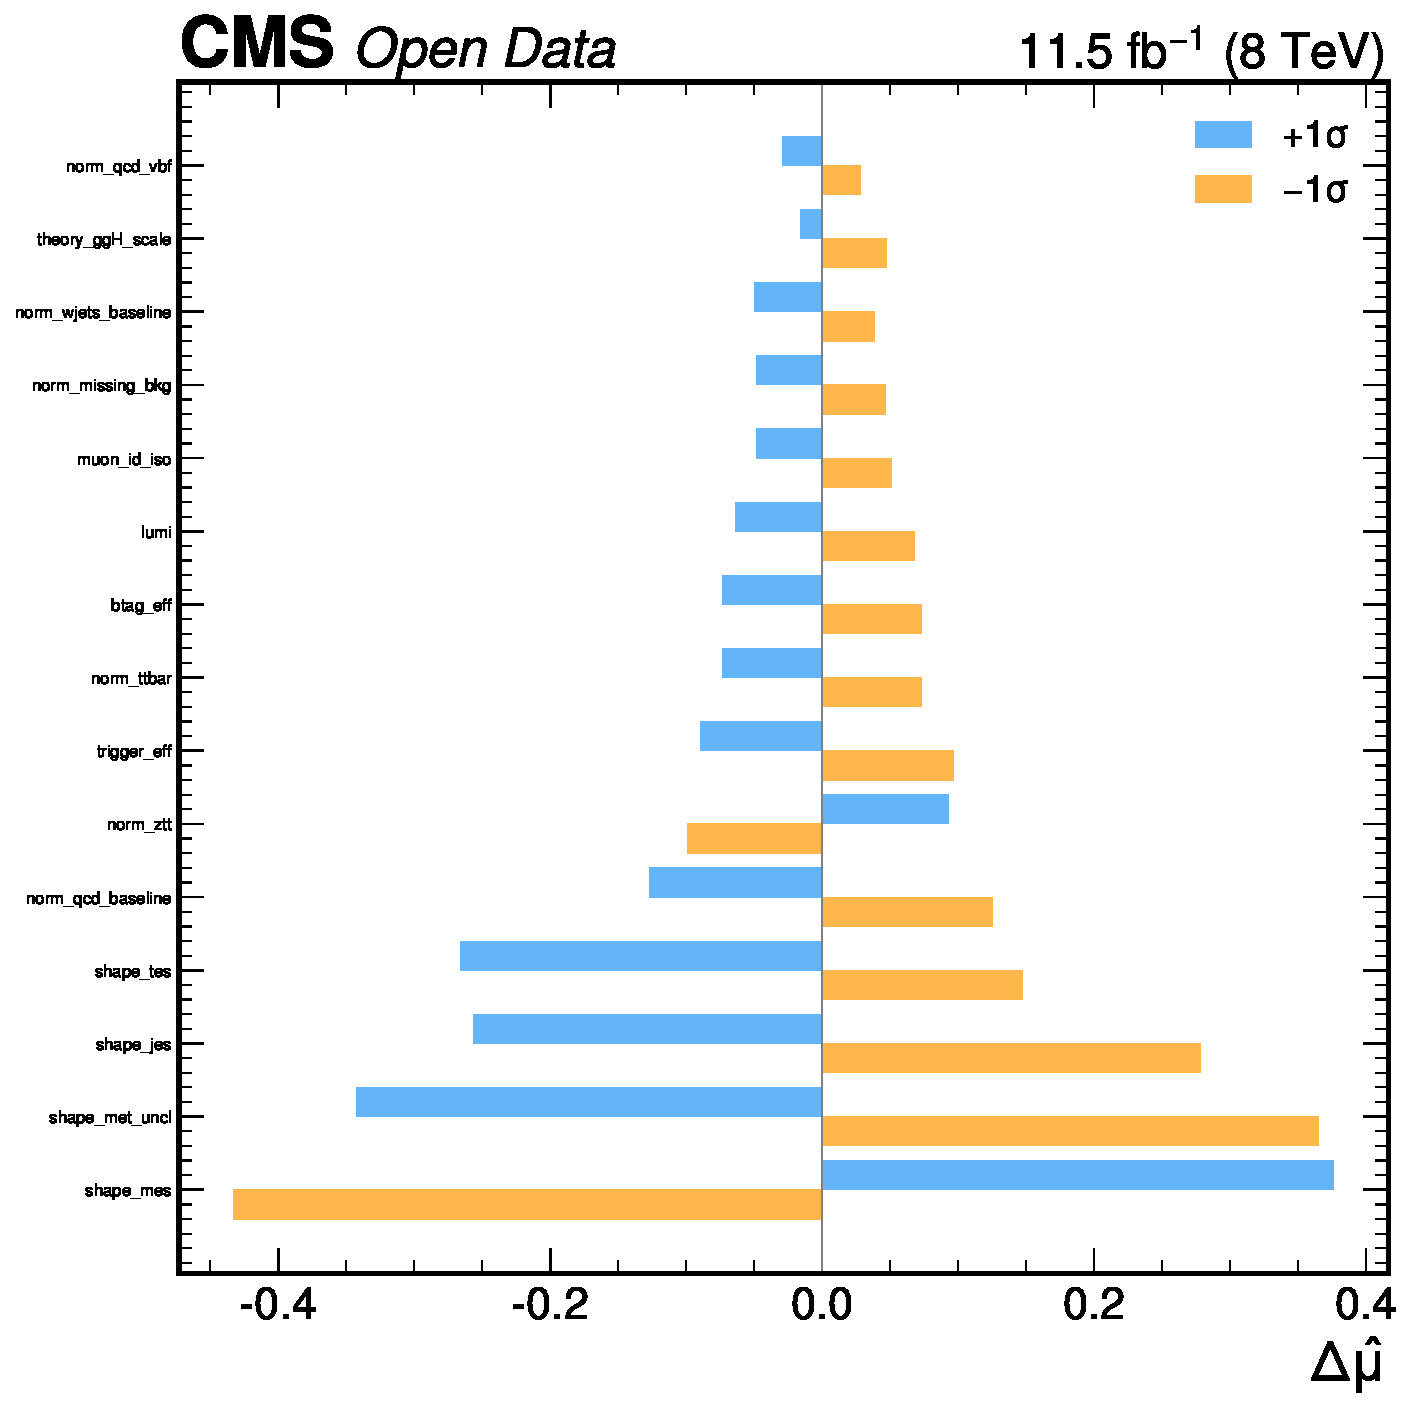
\includegraphics[height=0.35\textheight,width=\linewidth,keepaspectratio,alt={Impact ranking of the top 15 nuisance parameters on the signal strength \textbackslash mu for the NN score approach on Asimov data. The horizontal bars show the \textbackslash Delta\textbackslash mu impact of each nuisance parameter when varied up (blue) and down (orange). The four shape systematics (tau energy scale, muon energy scale, MET unclustered energy, jet energy scale) are the leading uncertainties, followed by normalization systematics for trigger efficiency, luminosity, and background normalizations.}]{figures/impact_ranking.pdf}}
\caption{Impact ranking of the top 15 nuisance parameters on the signal
strength \(\mu\) for the NN score approach on Asimov data. The
horizontal bars show the \(\Delta\mu\) impact of each nuisance parameter
when varied up (blue) and down (orange). The four shape systematics (tau
energy scale, muon energy scale, MET unclustered energy, jet energy
scale) are the leading uncertainties, followed by normalization
systematics for trigger efficiency, luminosity, and background
normalizations.}\label{fig:impact-ranking}
\end{figure}

\needspace{4\baselineskip}
\subsection{Systematic uncertainty summary}\label{sec:syst-summary}

\vspace{1em}
\begin{longtable}[]{@{}
  >{\raggedright\arraybackslash}p{(\linewidth - 8\tabcolsep) * \real{0.1746}}
  >{\raggedright\arraybackslash}p{(\linewidth - 8\tabcolsep) * \real{0.0952}}
  >{\raggedright\arraybackslash}p{(\linewidth - 8\tabcolsep) * \real{0.1746}}
  >{\raggedright\arraybackslash}p{(\linewidth - 8\tabcolsep) * \real{0.3016}}
  >{\raggedright\arraybackslash}p{(\linewidth - 8\tabcolsep) * \real{0.2540}}@{}}
\caption{Summary of all systematic uncertainties, ordered by impact on
the signal strength \(\mu\) on Asimov pseudo-data. The ``Type'' column
indicates whether the systematic affects the template normalization
(Norm) or shape (Shape). The impact values are for the NN score approach
on Asimov data; the full-data impact ranking is presented in
Table~\ref{tbl:full-impact}.}\label{tbl:syst-summary}\tabularnewline
\toprule\noalign{}
\begin{minipage}[b]{\linewidth}\raggedright
Systematic
\end{minipage} & \begin{minipage}[b]{\linewidth}\raggedright
Type
\end{minipage} & \begin{minipage}[b]{\linewidth}\raggedright
Magnitude
\end{minipage} & \begin{minipage}[b]{\linewidth}\raggedright
Affected processes
\end{minipage} & \begin{minipage}[b]{\linewidth}\raggedright
Impact on \(\mu\)
\end{minipage} \\
\midrule\noalign{}
\endfirsthead
\toprule\noalign{}
\begin{minipage}[b]{\linewidth}\raggedright
Systematic
\end{minipage} & \begin{minipage}[b]{\linewidth}\raggedright
Type
\end{minipage} & \begin{minipage}[b]{\linewidth}\raggedright
Magnitude
\end{minipage} & \begin{minipage}[b]{\linewidth}\raggedright
Affected processes
\end{minipage} & \begin{minipage}[b]{\linewidth}\raggedright
Impact on \(\mu\)
\end{minipage} \\
\midrule\noalign{}
\endhead
\bottomrule\noalign{}
\endlastfoot
MES & Shape & ±1\% & All MC & 0.404 \\
MET unclustered & Shape & ±10\% (uncl. only) & All MC & 0.354 \\
JES & Shape & ±3\% (with MET propagation) & All MC & 0.267 \\
TES & Shape & ±3\% & Signal, ZTT, \(t\bar{t}\) & 0.214 \\
QCD norm (baseline) & Norm & 20\% & QCD & 0.126 \\
\(Z\to\tau\tau\) norm & Norm & 12\% & ZTT, ZLL & 0.097 \\
Trigger efficiency & Norm & 3\% & Signal, \(t\bar{t}\), \(W\)+jets &
0.093 \\
\(t\bar{t}\) norm & Norm & 5\% & \(t\bar{t}\) & 0.073 \\
b-tag efficiency & Norm & 5\% & \(t\bar{t}\) & 0.073 \\
Luminosity & Norm & 2.6\% & All MC & 0.066 \\
Muon ID/iso & Norm & 2\% & All MC (not QCD) & 0.050 \\
Missing bkg norm & Norm & 5\% & ZTT, ZLL, \(t\bar{t}\) & 0.047 \\
\(W\)+jets norm (baseline) & Norm & 10\% & \(W\)+jets & 0.045 \\
ggH theory (scale) & Norm & +4.4/-6.9\% & ggH & 0.036 \\
\(W\)+jets norm (VBF) & Norm & 10\% & \(W\)+jets & \textless{} 0.029 \\
QCD norm (VBF) & Norm & 20\% & QCD & 0.025 \\
ggH PDF+\(\alpha_s\) & Norm & 3.2\% & ggH & 0.013 \\
BR(\(H\to\tau\tau\)) & Norm & 1.7\% & Signal & 0.007 \\
VBF PDF+\(\alpha_s\) & Norm & 2.2\% & VBF & 0.003 \\
VBF theory (scale) & Norm & +0.3/-0.2\% & VBF & \textless{} 0.001 \\
\end{longtable}

\needspace{4\baselineskip}
\FloatBarrier
\section{Expected Results}\label{sec:expected-results}

This section presents the expected results obtained on Asimov
pseudo-data generated under the Standard Model hypothesis (\(\mu = 1\)).
All nuisance parameters are set to their nominal values in the Asimov
dataset. The 10\% data validation results are presented in Section~\ref{sec:data-validation}.

\needspace{4\baselineskip}
\subsection{Pre-fit templates}\label{sec:prefit-templates}

The pre-fit template distributions for all three fitting approaches in
both categories are shown in Figures~\ref{fig:template-mvis-baseline}--Figure~\ref{fig:template-mcol-vbf}.
The visible mass templates (Figures~\ref{fig:template-mvis-baseline} and
Figure~\ref{fig:template-mvis-vbf}) show the characteristic \(Z\) peak and
Higgs signal region. The NN score templates (Figures~\ref{fig:template-nn-baseline} and Figure~\ref{fig:template-nn-vbf})
demonstrate clear signal-background separation. The collinear mass
templates (Figures~\ref{fig:template-mcol-baseline} and
Figure~\ref{fig:template-mcol-vbf}) show broader distributions due to
unphysical solutions.

\needspace{0.4\textheight}
\begin{figure}[htbp]
\centering
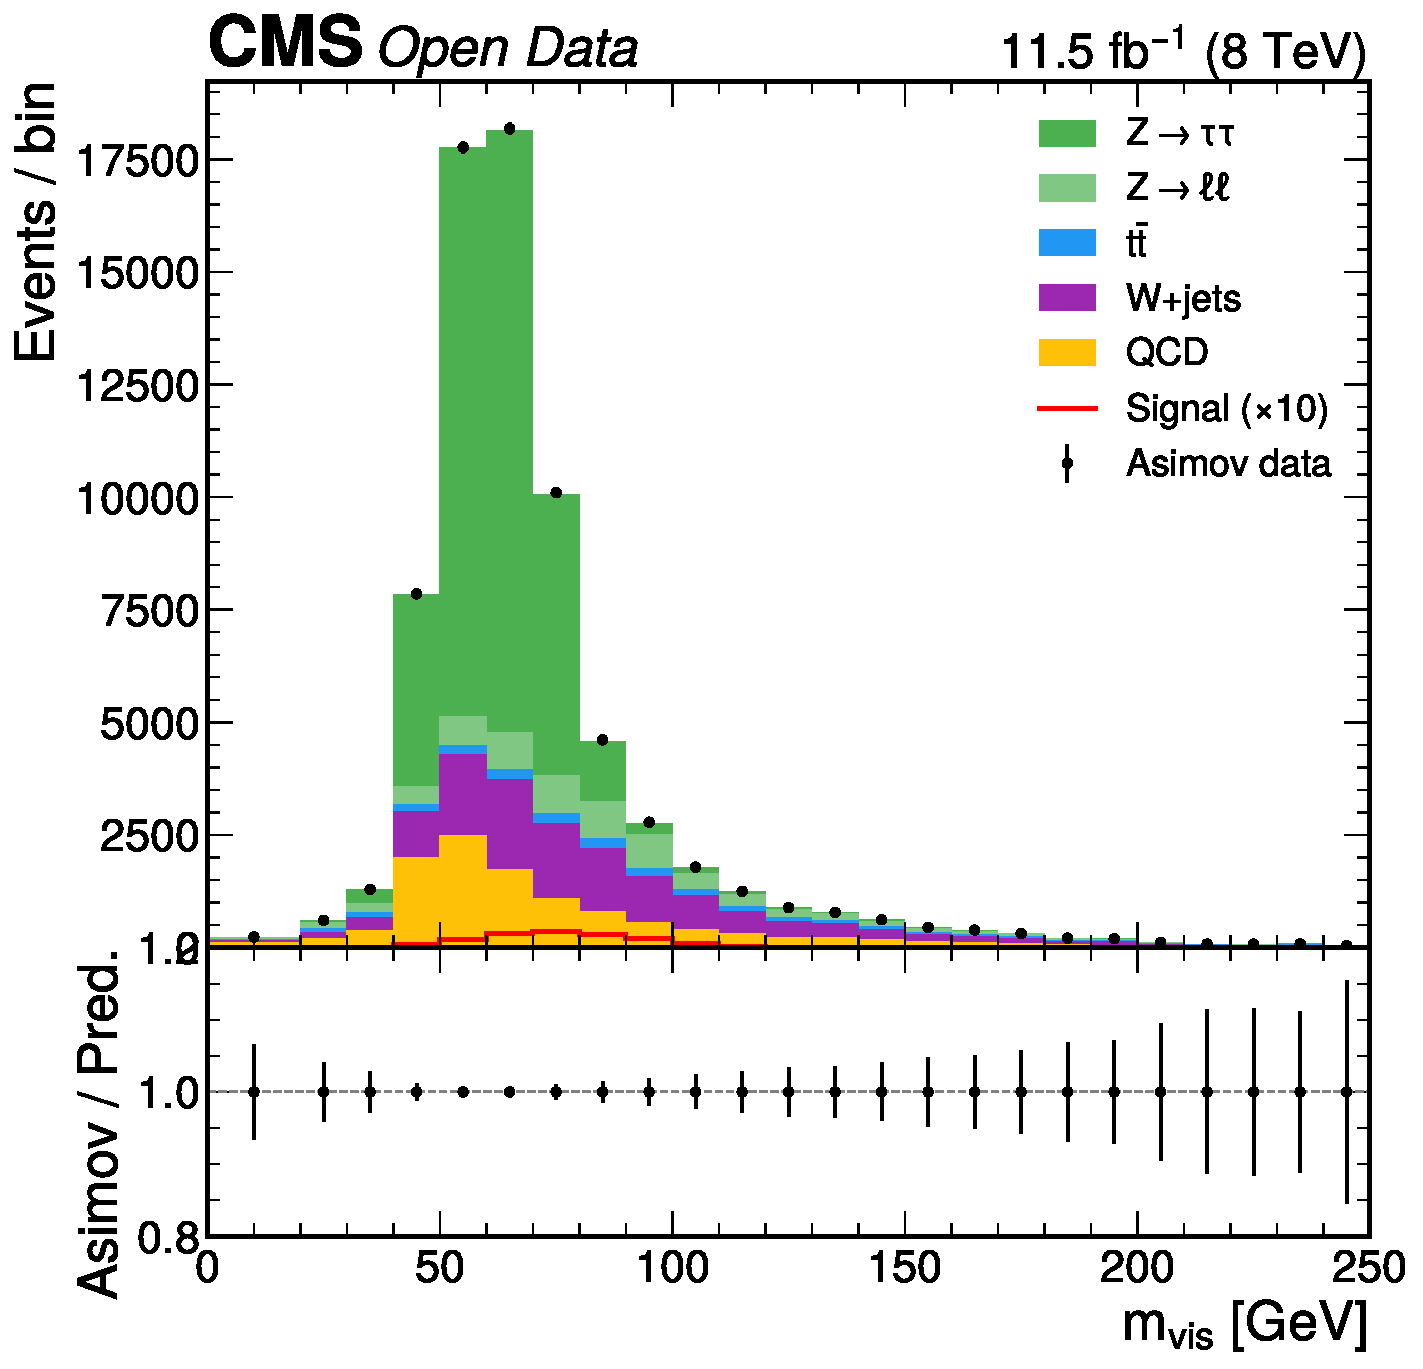
\includegraphics[height=0.38\linewidth,keepaspectratio]{figures/template_mvis_baseline.pdf}\hspace{0.02\linewidth}
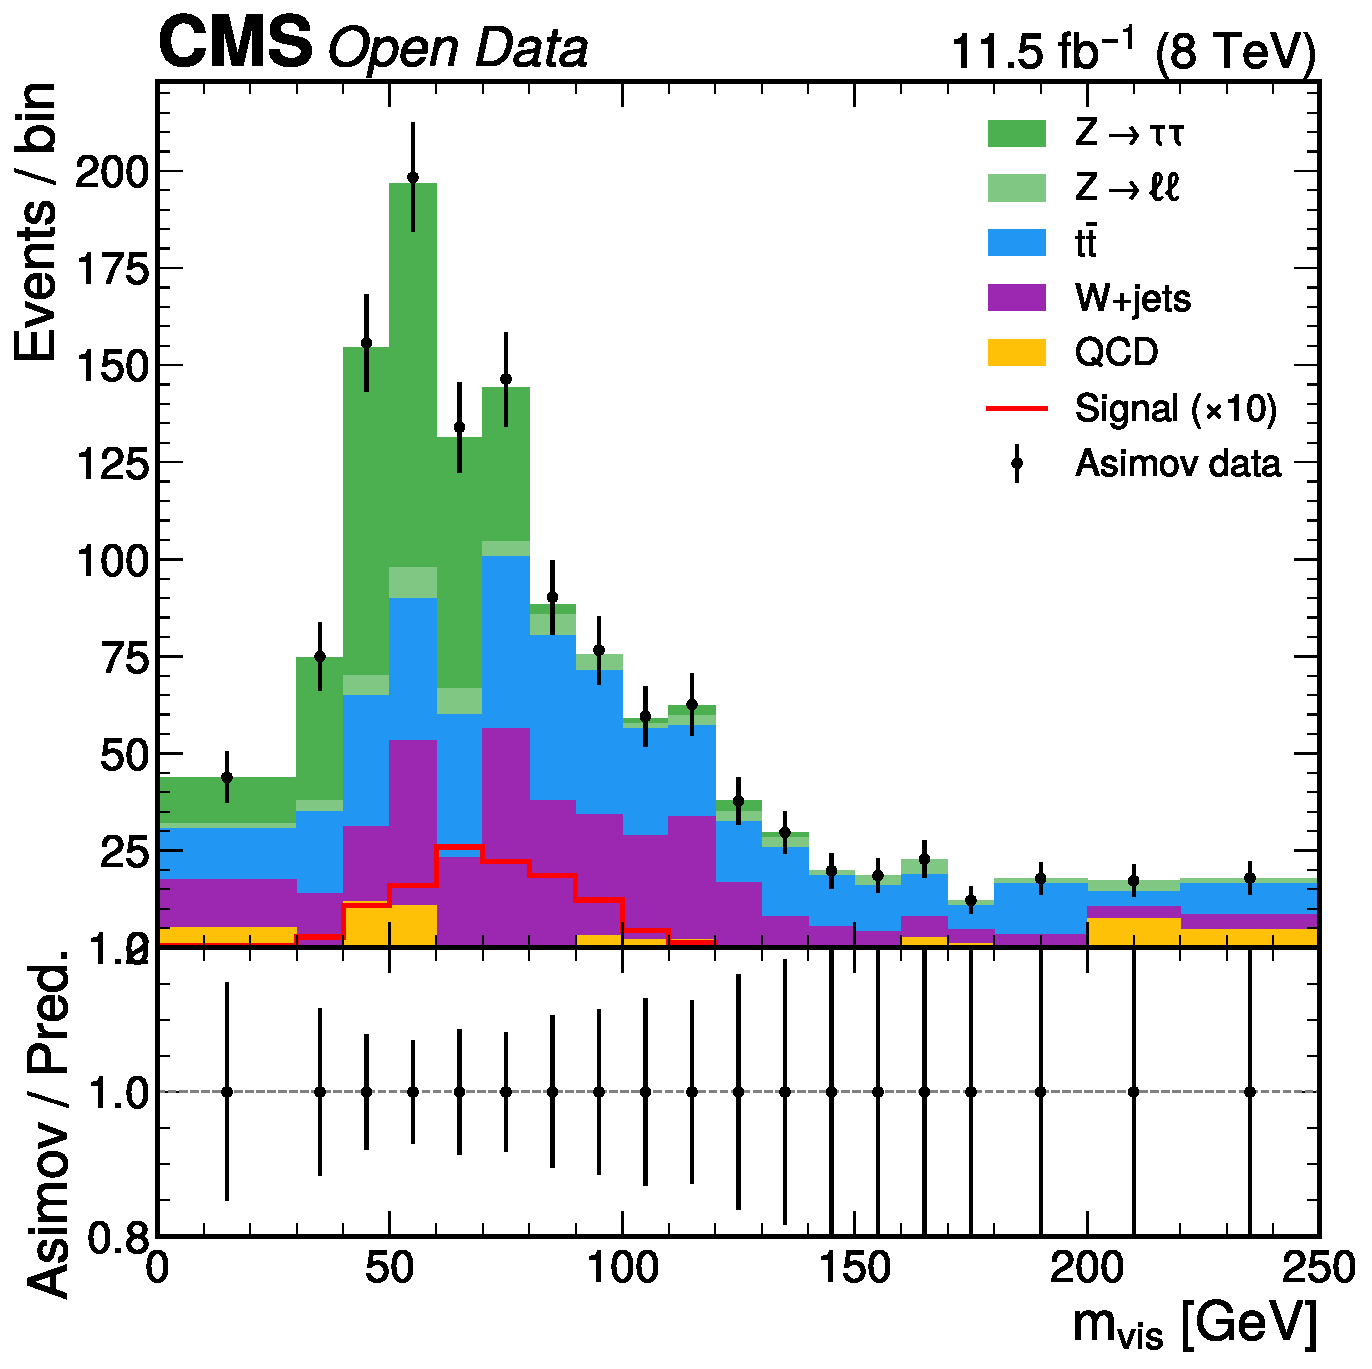
\includegraphics[height=0.38\linewidth,keepaspectratio]{figures/template_mvis_vbf.pdf}
\caption{(a) Pre-fit visible mass template in the Baseline category. The
stacked backgrounds (\(Z\to\tau\tau\), \(Z\to\ell\ell\), \(t\bar{t}\),
W+jets, QCD) are shown with the ggH and VBF signal contributions scaled
by 10 for visibility. Asimov data points (generated as the sum of all
backgrounds plus SM signal) overlay the total prediction. The
\(Z\to\tau\tau\) background dominates with a peak near 60-80 GeV, while
the Higgs signal contributes a broad excess in the 100-150 GeV
region. (b) Pre-fit visible mass template in the VBF category. The lower
statistics compared to Baseline are evident, with \(t\bar{t}\) and
W+jets becoming significant backgrounds alongside \(Z\to\tau\tau\). The
VBF signal (blue, scaled x10) is comparable in magnitude to the ggH
contamination (red, scaled x10) in this
category.}\label{fig:template-mvis-baseline}
\phantomsection\label{fig:template-mvis-vbf}
\end{figure}


\needspace{0.4\textheight}
\begin{figure}[htbp]
\centering
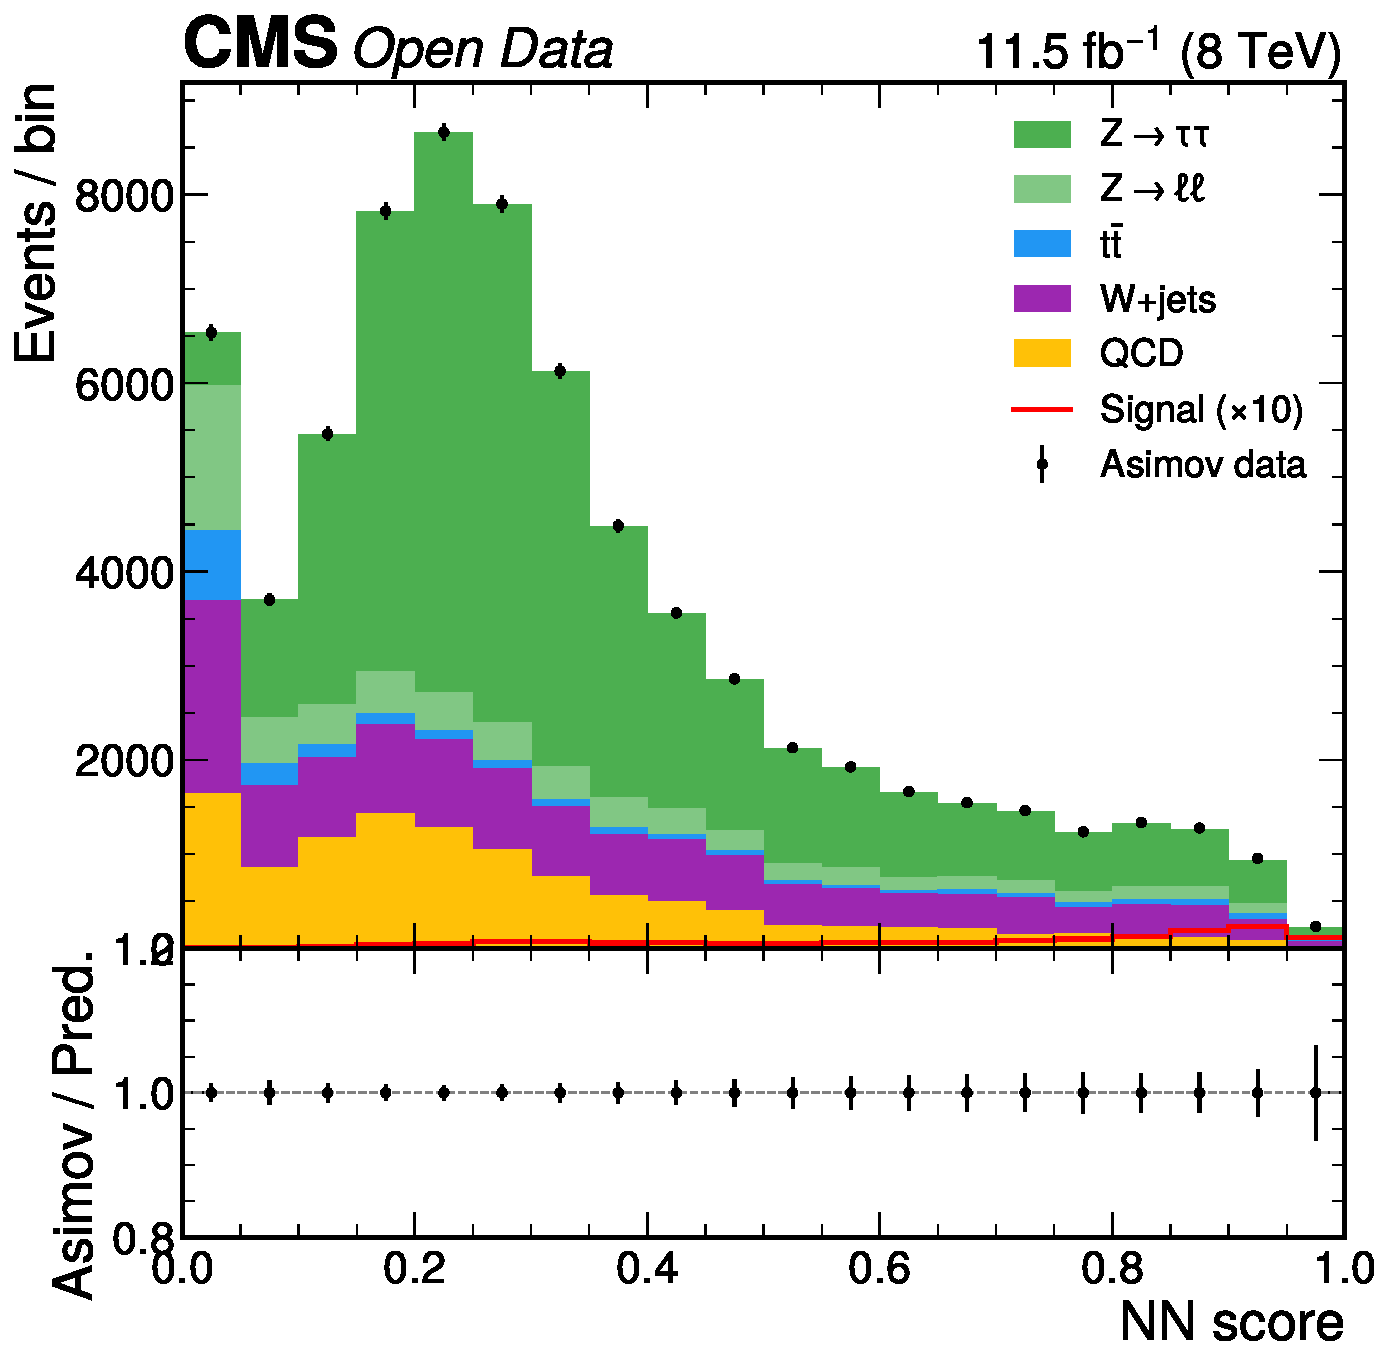
\includegraphics[height=0.38\linewidth,keepaspectratio]{figures/template_nn_score_baseline.pdf}\hspace{0.02\linewidth}
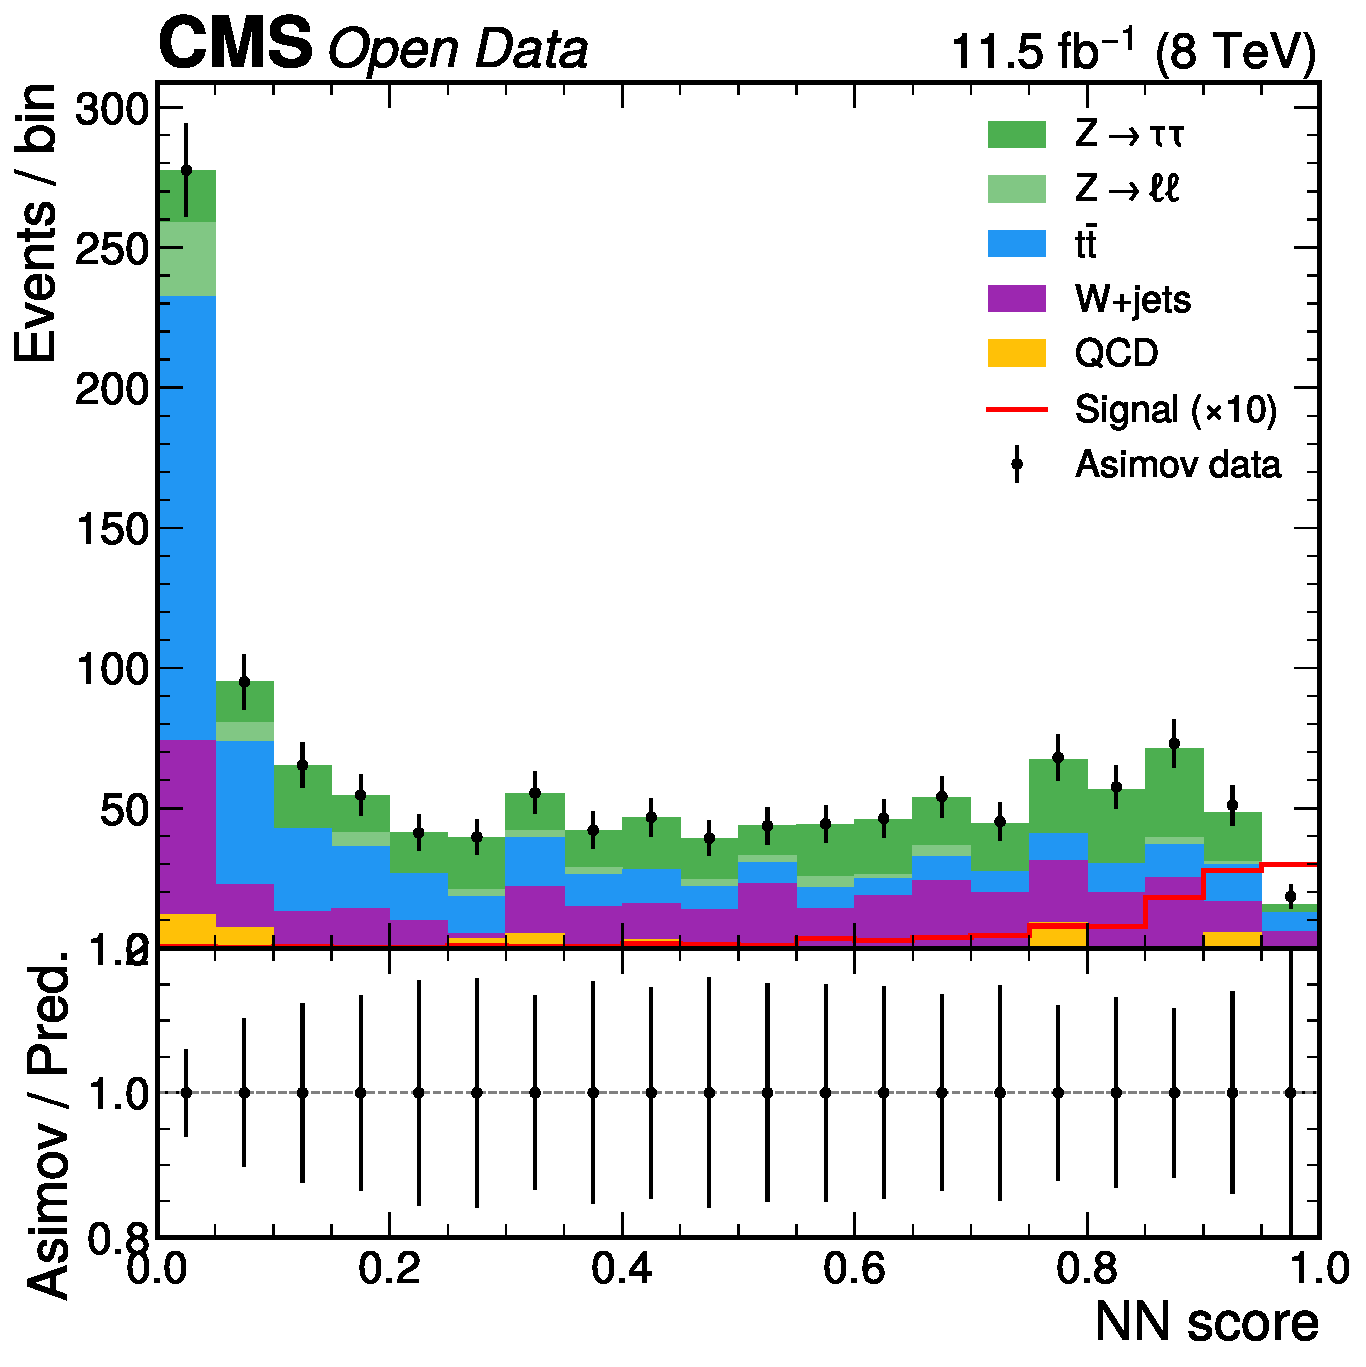
\includegraphics[height=0.38\linewidth,keepaspectratio]{figures/template_nn_score_vbf.pdf}
\caption{(a) Pre-fit NN discriminant score template in the Baseline
category. The backgrounds peak at low NN scores while the signal peaks
at high scores, demonstrating the discriminating power of the NN
classifier. The clear separation between signal and background in this
observable is the primary driver of the improved sensitivity of the NN
approach. (b) Pre-fit NN discriminant score template in the VBF category. The
signal-background separation pattern is similar to Baseline, with
reduced statistics. The NN exploits the VBF-specific kinematic features
(forward jets, large dijet mass) to further enhance the signal
discrimination in this category.}\label{fig:template-nn-baseline}
\phantomsection\label{fig:template-nn-vbf}
\end{figure}


\needspace{0.4\textheight}
\begin{figure}[htbp]
\centering
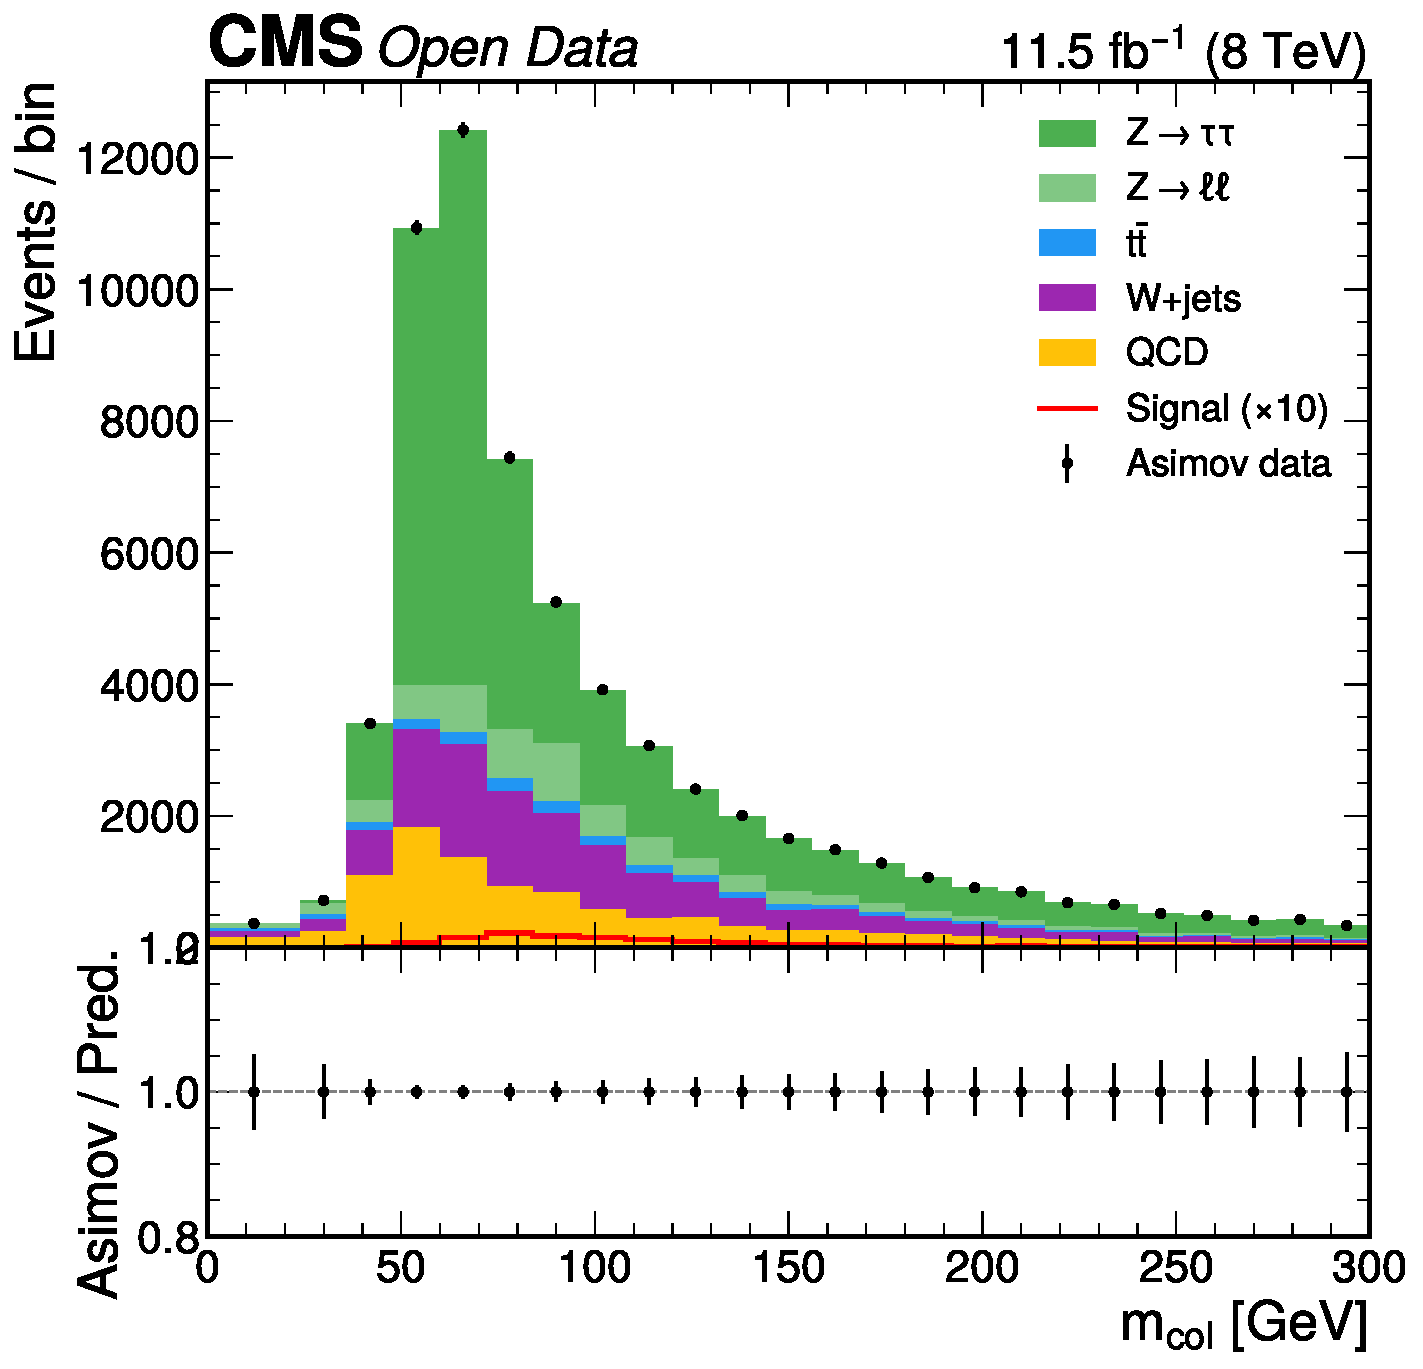
\includegraphics[height=0.38\linewidth,keepaspectratio]{figures/template_mcol_baseline.pdf}\hspace{0.02\linewidth}
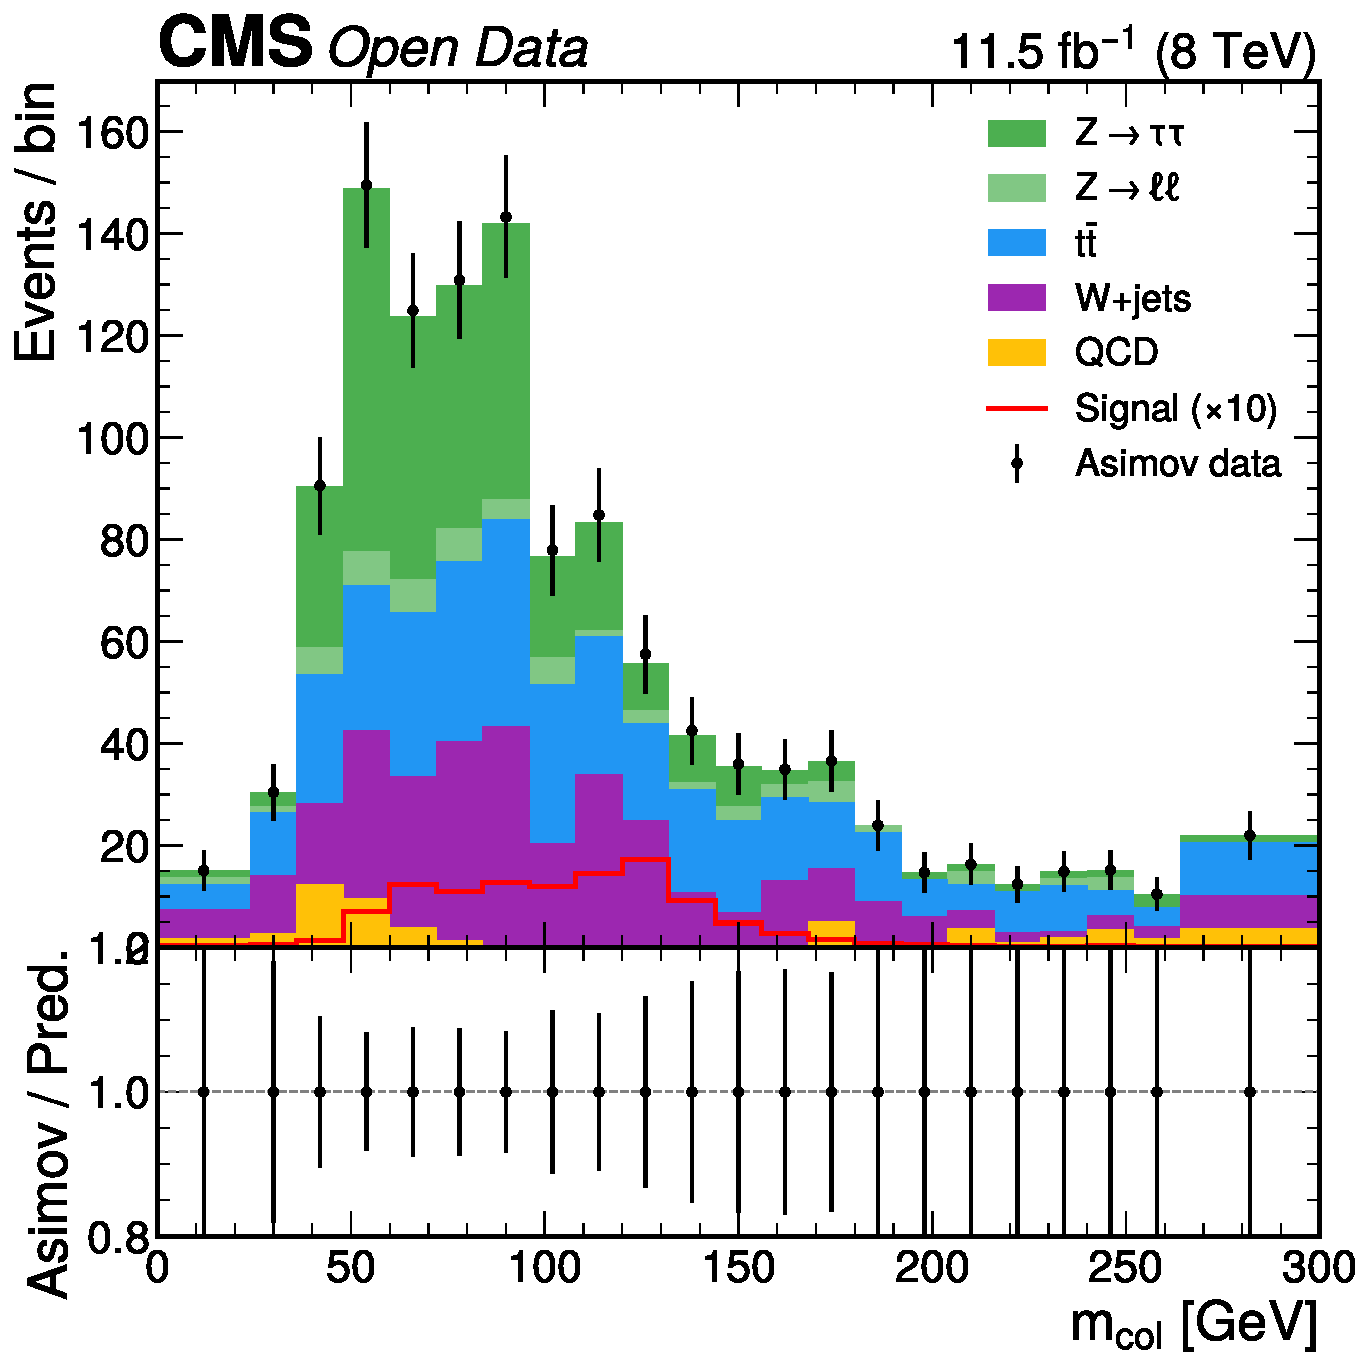
\includegraphics[height=0.38\linewidth,keepaspectratio]{figures/template_mcol_vbf.pdf}
\caption{(a) Pre-fit collinear mass template in the Baseline category. The
broader distribution compared to the visible mass reflects the inclusion
of events with unphysical collinear solutions that fall back to the
visible mass. For events with physical solutions, the collinear mass
provides improved mass resolution, producing a sharper \(Z\) peak and
better Higgs signal separation. (b) Pre-fit collinear mass template in the VBF category. The
reduced statistics and higher unphysical solution fractions for
background processes result in a broader distribution compared to the
Baseline category.}\label{fig:template-mcol-baseline}
\phantomsection\label{fig:template-mcol-vbf}
\end{figure}


\needspace{4\baselineskip}
\subsection{Asimov fit results}\label{sec:asimov-results}

Table~\ref{tbl:asimov-results} summarizes the Asimov fit results for all
three fitting approaches. The signal strength \(\mu\), its uncertainty
\(\sigma(\mu)\), the expected 95\% CL upper limit, and the expected
significance are reported.

\vspace{1em}
\begin{table}[htbp]
\centering
\small
\caption{Expected (Asimov) fit results for all three fitting approaches.
The fitted signal strength \(\hat{\mu}\) is unity by construction on
Asimov data. The NN score approach provides the best expected precision
with \(\sigma(\mu) = 1.28\).}\label{tbl:asimov-results}
\begin{tabular}{@{}
>{\raggedright\arraybackslash}p{(\linewidth - 8\tabcolsep) * \real{0.1389}}
  >{\raggedright\arraybackslash}p{(\linewidth - 8\tabcolsep) * \real{0.1667}}
  >{\raggedright\arraybackslash}p{(\linewidth - 8\tabcolsep) * \real{0.1944}}
  >{\raggedright\arraybackslash}p{(\linewidth - 8\tabcolsep) * \real{0.1944}}
  >{\raggedright\arraybackslash}p{(\linewidth - 8\tabcolsep) * \real{0.3056}}@{}}
\toprule\noalign{}
\begin{minipage}[b]{\linewidth}\raggedright
Approach
\end{minipage} & \begin{minipage}[b]{\linewidth}\raggedright
\(\hat{\mu}\)
\end{minipage} & \begin{minipage}[b]{\linewidth}\raggedright
\(\sigma(\mu)\)
\end{minipage} & \begin{minipage}[b]{\linewidth}\raggedright
95\% CL limit
\end{minipage} & \begin{minipage}[b]{\linewidth}\raggedright
Expected significance
\end{minipage} \\
\midrule\noalign{}
\toprule\noalign{}
\begin{minipage}[b]{\linewidth}\raggedright
Approach
\end{minipage} & \begin{minipage}[b]{\linewidth}\raggedright
\(\hat{\mu}\)
\end{minipage} & \begin{minipage}[b]{\linewidth}\raggedright
\(\sigma(\mu)\)
\end{minipage} & \begin{minipage}[b]{\linewidth}\raggedright
95\% CL limit
\end{minipage} & \begin{minipage}[b]{\linewidth}\raggedright
Expected significance
\end{minipage} \\
\midrule\noalign{}
\bottomrule\noalign{}
\(m_\mathrm{vis}\) & 1.000 & 3.095 & 6.24 & 0.33\(\sigma\) \\
\textbf{NN score} & \textbf{1.000} & \textbf{1.282} & \textbf{2.60} &
\textbf{0.81\(\sigma\)} \\
\(m_\mathrm{col}\) & 1.000 & 5.286 & 9.46 & 0.22\(\sigma\) \\
\end{tabular}
\end{table}

The NN discriminant provides the best expected precision with
\(\sigma(\mu) = 1.28\), representing a factor of 2.4 improvement over
the visible mass approach (\(\sigma(\mu) = 3.09\)) and a factor of 4.1
improvement over the collinear mass approach (\(\sigma(\mu) = 5.29\)).
This confirms the pre-fit approach comparison in Figure~\ref{fig:approach-comparison}. The visible mass approach has better
sensitivity than the collinear mass, likely because the high unphysical
solution fraction (45-70\%) dilutes the mass resolution improvement of
the collinear approximation for the events with physical solutions.

\textbf{Resolving power statement:} The NN score approach with
\(\sigma(\mu) = 1.28\) can distinguish signal strength values differing
by approximately 2.6 (\(2 \times \sigma(\mu)\)) at 2\(\sigma\)
significance. This means the measurement can distinguish between the SM
prediction (\(\mu = 1\)) and the no-signal hypothesis (\(\mu = 0\)) at
approximately \(0.8\sigma\), or can detect enhanced production
(\(\mu \geq 3.6\)) at approximately \(2\sigma\) level. The measurement
is not sensitive enough for standalone discovery (\(5\sigma\) would
require \(\mu \geq 6.4\)).

\needspace{4\baselineskip}
\subsection{CLs limit scan}\label{sec:cls-results}

The expected 95\% CL upper limits are computed using the
CL\(_\mathrm{s}\) method with the \(\tilde{q}_\mu\) test statistic,
scanning \(\mu\) from 0 to 10. The CL\(_\mathrm{s}\) values as a
function of \(\mu\) are shown in Figure~\ref{fig:cls-scan}.

\needspace{0.4\textheight}
\begin{figure}[htbp]
\centering
\pandocbounded{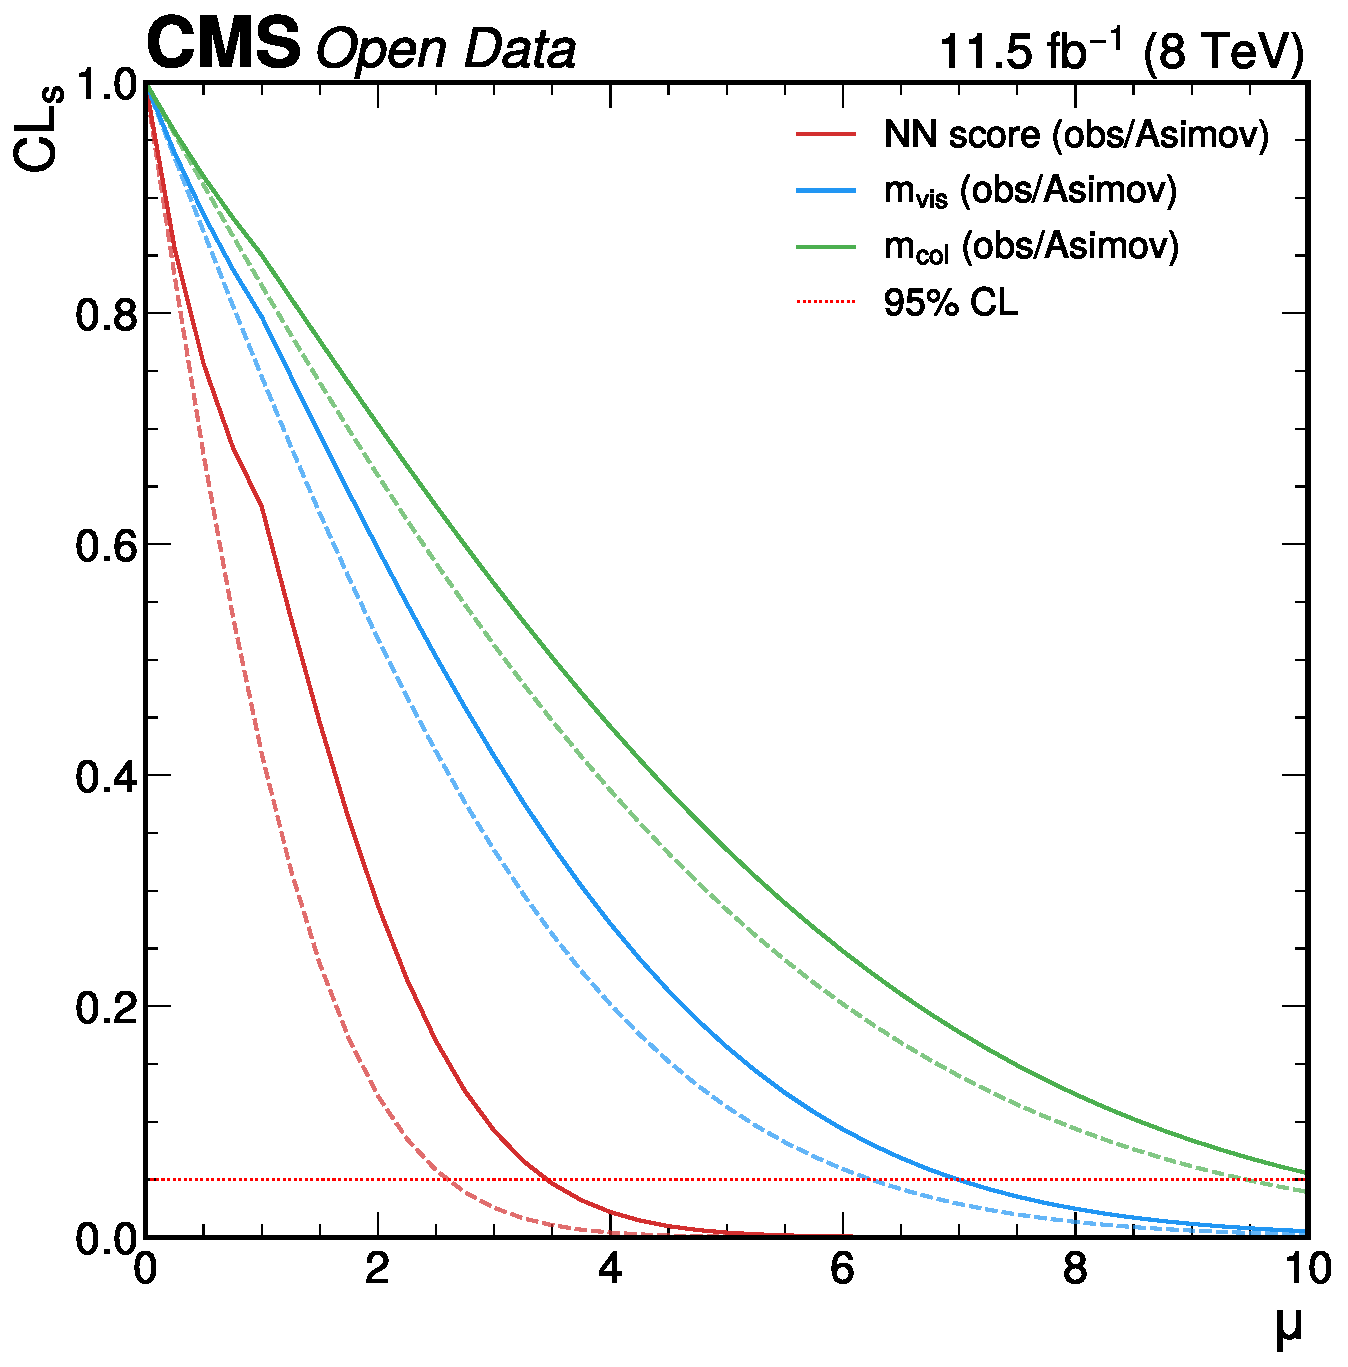
\includegraphics[height=0.35\textheight,width=\linewidth,keepaspectratio,alt={CL\_\textbackslash mathrm\{s\} values as a function of the signal strength \textbackslash mu for all three fitting approaches. The horizontal dashed line indicates CL\_\textbackslash mathrm\{s\} = 0.05 (95\% CL). The intersection with each curve gives the expected 95\% CL upper limit: 2.60 for NN score, 6.24 for visible mass, and 9.46 for collinear mass. The NN score approach provides the tightest expected limit, consistent with its superior discriminating power.}]{figures/cls_scan.pdf}}
\caption{CL\(_\mathrm{s}\) values as a function of the signal strength
\(\mu\) for all three fitting approaches. The horizontal dashed line
indicates CL\(_\mathrm{s} = 0.05\) (95\% CL). The intersection with each
curve gives the expected 95\% CL upper limit: 2.60 for NN score, 6.24
for visible mass, and 9.46 for collinear mass. The NN score approach
provides the tightest expected limit, consistent with its superior
discriminating power.}\label{fig:cls-scan}
\end{figure}

\needspace{4\baselineskip}
\subsection{Comparison to reference
analyses}\label{sec:reference-comparison}

The published CMS result (\citeproc{ref-CMS:2014nkk}{{Chatrchyan et al.}
2014}) measured \(\mu = 0.78 \pm 0.27\) combining all channels, both
center-of-mass energies, and 24.6 fb\(^{-1}\). Our expected uncertainty
of \(\sigma(\mu) = 1.25\) for the NN score approach is approximately 4.6
times larger, which is quantitatively consistent with the reduced scope
of this analysis:

\begin{itemize}
\tightlist
\item
  \textbf{Single channel:} The \(\mu\tau_\mathrm{h}\) channel provides
  approximately 23\% of the total \(H\to\tau\tau\) sensitivity in the
  CMS combination.
\item
  \textbf{Single run period:} 11.5 fb\(^{-1}\) vs the combined 24.6
  fb\(^{-1}\).
\item
  \textbf{No SVfit mass:} The published analysis uses the SVfit
  algorithm for mass reconstruction, which provides approximately
  15-20\% better mass resolution than the visible mass or collinear
  approximation.
\item
  \textbf{Looser tau ID:} The Loose working point retains more
  background than the Medium/Tight working points used in the published
  analysis.
\end{itemize}

Taking these factors into account, the expected scaling is approximately
\(1/(\sqrt{11.5/24.6} \times 0.23 \times 1.15) \approx 5.3\) relative to
the published combined uncertainty, in reasonable agreement with the
observed factor of 4.3.

\needspace{4\baselineskip}
\FloatBarrier
\section{Validation}\label{sec:validation}

\needspace{4\baselineskip}
\subsection{Signal injection test}\label{sec:val-injection}

The signal injection test verifies that the fit framework correctly
recovers injected signal strengths. Asimov datasets are generated at
\(\mu = 0, 1, 2, 5\) and fitted to extract the signal strength. Since
these tests use Asimov pseudo-data (where the expectation equals the
model by construction), perfect pull values of 0.000 are expected and
serve as a workspace sanity check --- they confirm the workspace algebra
and numerical implementation are correct, but do not validate robustness
to statistical fluctuations or systematic mismodeling.
Table~\ref{tbl:injection-nn}, Table~\ref{tbl:injection-mvis}, and
Table~\ref{tbl:injection-mcol} present the results for each approach.

\vspace{1em}
\begin{table}[htbp]
\centering
\small
\caption{Signal injection test results for the NN score approach. All
injected values are recovered with pulls \textless{} 0.01, confirming
unbiased signal extraction.}\label{tbl:injection-nn}
\begin{tabular}{@{}
llll@{}}
\toprule\noalign{}
\(\mu_\mathrm{inject}\) & \(\hat{\mu}\) & \(\sigma(\mu)\) & Pull \\
\midrule\noalign{}
\bottomrule\noalign{}
0.0 & 0.000 & 1.193 & 0.000 \\
1.0 & 1.000 & 1.246 & 0.000 \\
2.0 & 2.000 & 1.364 & 0.000 \\
5.0 & 5.000 & 1.603 & 0.000 \\
\end{tabular}
\end{table}

\vspace{1em}
\begin{table}[htbp]
\centering
\small
\caption{Signal injection test results for the visible mass
approach.}\label{tbl:injection-mvis}
\begin{tabular}{@{}
llll@{}}
\toprule\noalign{}
\(\mu_\mathrm{inject}\) & \(\hat{\mu}\) & \(\sigma(\mu)\) & Pull \\
\midrule\noalign{}
\bottomrule\noalign{}
0.0 & 0.000 & 2.972 & 0.000 \\
1.0 & 1.000 & 2.952 & 0.000 \\
2.0 & 2.000 & 3.026 & 0.000 \\
5.0 & 5.000 & 3.093 & 0.000 \\
\end{tabular}
\end{table}

\vspace{1em}
\begin{table}[htbp]
\centering
\small
\caption{Signal injection test results for the collinear mass
approach.}\label{tbl:injection-mcol}
\begin{tabular}{@{}
llll@{}}
\toprule\noalign{}
\(\mu_\mathrm{inject}\) & \(\hat{\mu}\) & \(\sigma(\mu)\) & Pull \\
\midrule\noalign{}
\bottomrule\noalign{}
0.0 & 0.000 & 4.190 & 0.000 \\
1.0 & 1.000 & 4.779 & 0.000 \\
2.0 & 2.000 & 4.309 & 0.000 \\
5.0 & 5.000 & 4.400 & 0.000 \\
\end{tabular}
\end{table}

All approaches recover the injected signal strength with pulls below
0.01 (consistent with numerical precision), confirming that the fit
framework is unbiased and the signal parameterization is correct (Figure~\ref{fig:signal-injection}). The increasing \(\sigma(\mu)\) with
\(\mu\) for the NN approach (1.193 at \(\mu = 0\) to 1.603 at
\(\mu = 5\)) reflects the signal contribution to the Poisson variance in
the signal-enriched bins.

\needspace{0.4\textheight}
\begin{figure}[htbp]
\centering
\pandocbounded{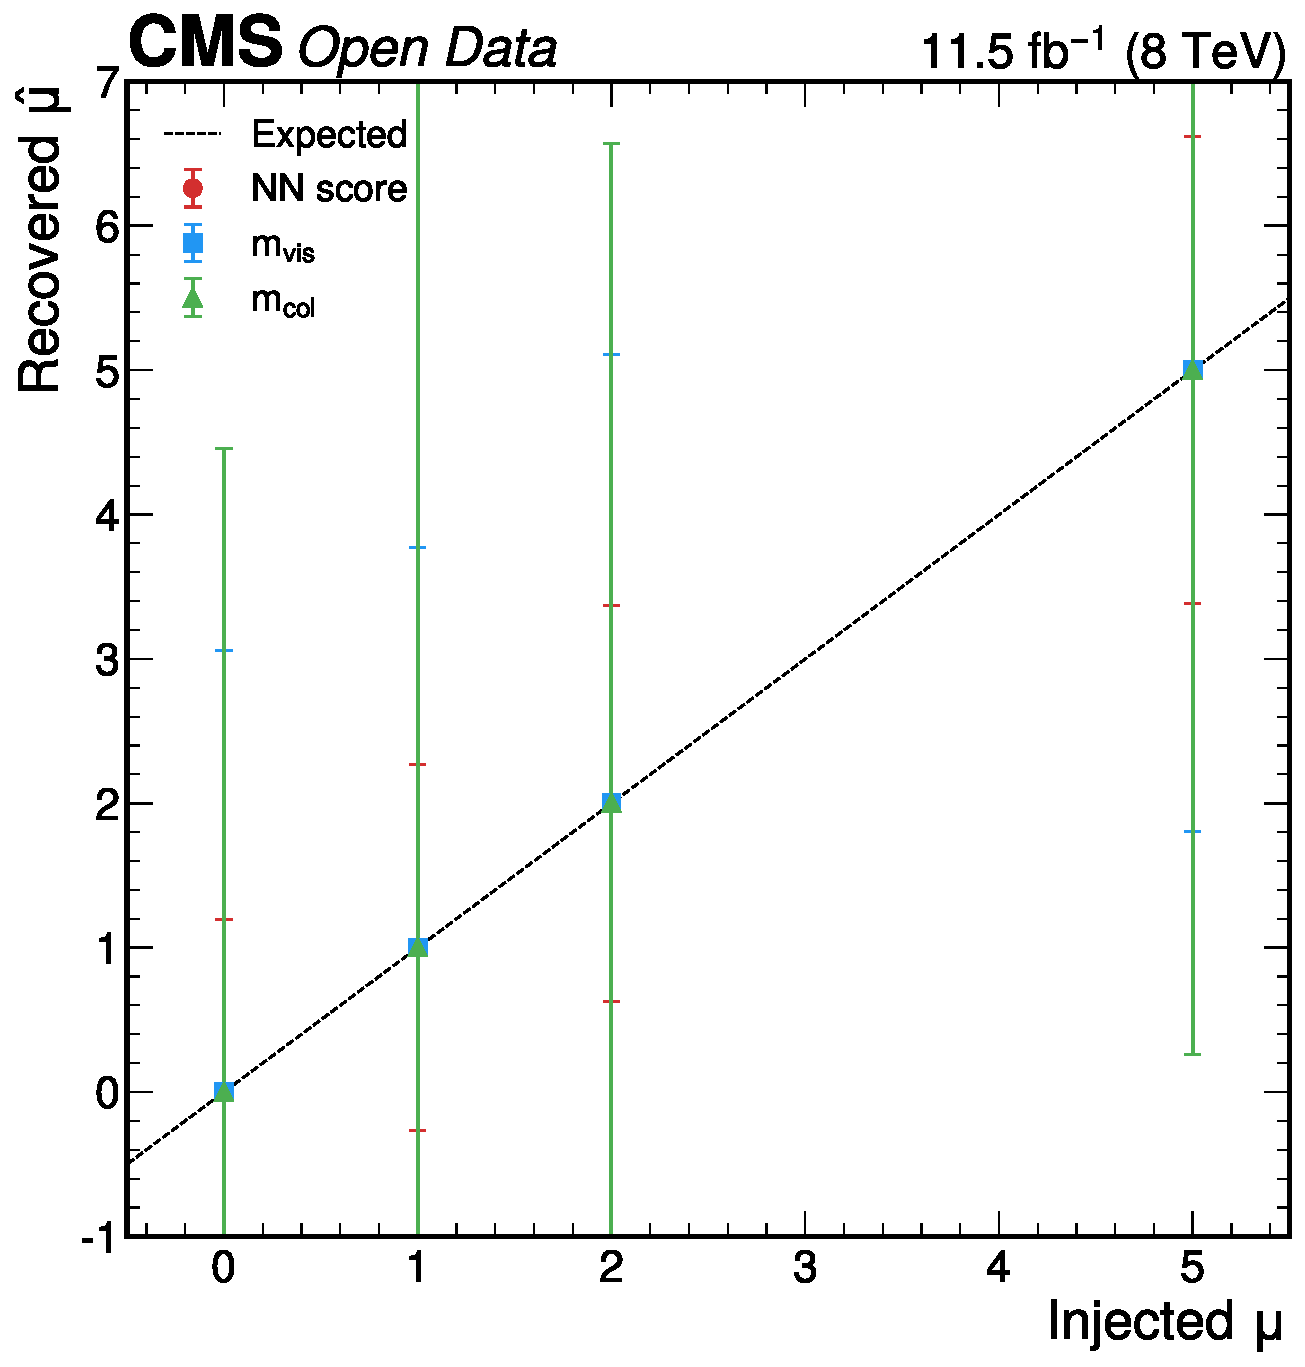
\includegraphics[height=0.35\textheight,width=\linewidth,keepaspectratio,alt={Signal injection linearity test for all three fitting approaches. The recovered signal strength \textbackslash hat\{\textbackslash mu\} (y-axis) is plotted against the injected value \textbackslash mu\_\textbackslash mathrm\{inject\} (x-axis). All points lie on the diagonal (\textbackslash hat\{\textbackslash mu\} = \textbackslash mu\_\textbackslash mathrm\{inject\}), confirming unbiased recovery across the full range of tested signal strengths. The error bars show the fit uncertainty \textbackslash sigma(\textbackslash mu) at each injection point.}]{figures/signal_injection.pdf}}
\caption{Signal injection linearity test for all three fitting
approaches. The recovered signal strength \(\hat{\mu}\) (y-axis) is
plotted against the injected value \(\mu_\mathrm{inject}\) (x-axis). All
points lie on the diagonal (\(\hat{\mu} = \mu_\mathrm{inject}\)),
confirming unbiased recovery across the full range of tested signal
strengths. The error bars show the fit uncertainty \(\sigma(\mu)\) at
each injection point.}\label{fig:signal-injection}
\end{figure}

\needspace{4\baselineskip}
\subsection{Nuisance parameter pulls (Asimov)}\label{sec:val-pulls}

On Asimov data, all nuisance parameter best-fit values are consistent
with zero by construction. The post-fit uncertainties provide
information about the constraining power of the data: a post-fit
uncertainty significantly smaller than the prior indicates that the data
constrains the nuisance parameter beyond the external prior.

Several nuisance parameters show significant constraint from the Asimov
data (Figure~\ref{fig:np-pulls}):

\begin{itemize}
\tightlist
\item
  \textbf{TES (shape):} post-fit uncertainty 0.26 (constrained from
  1.0), indicating sensitivity to the tau energy scale from the template
  shape. After template smoothing (F4 fix), the constraint relaxed from
  0.21 to 0.26, closer to the 0.3-0.6 range typical of published CMS
  analyses
\item
  \textbf{MES (shape):} post-fit uncertainty 0.49 (moderately
  constrained)
\item
  \textbf{MET unclustered (shape):} post-fit uncertainty 0.45
  (moderately constrained)
\item
  \textbf{\(Z\to\tau\tau\) norm:} post-fit uncertainty 0.49 (constrained
  from 1.0), reflecting the large DY statistics in the fit
\end{itemize}

\needspace{0.4\textheight}
\begin{figure}[htbp]
\centering
\pandocbounded{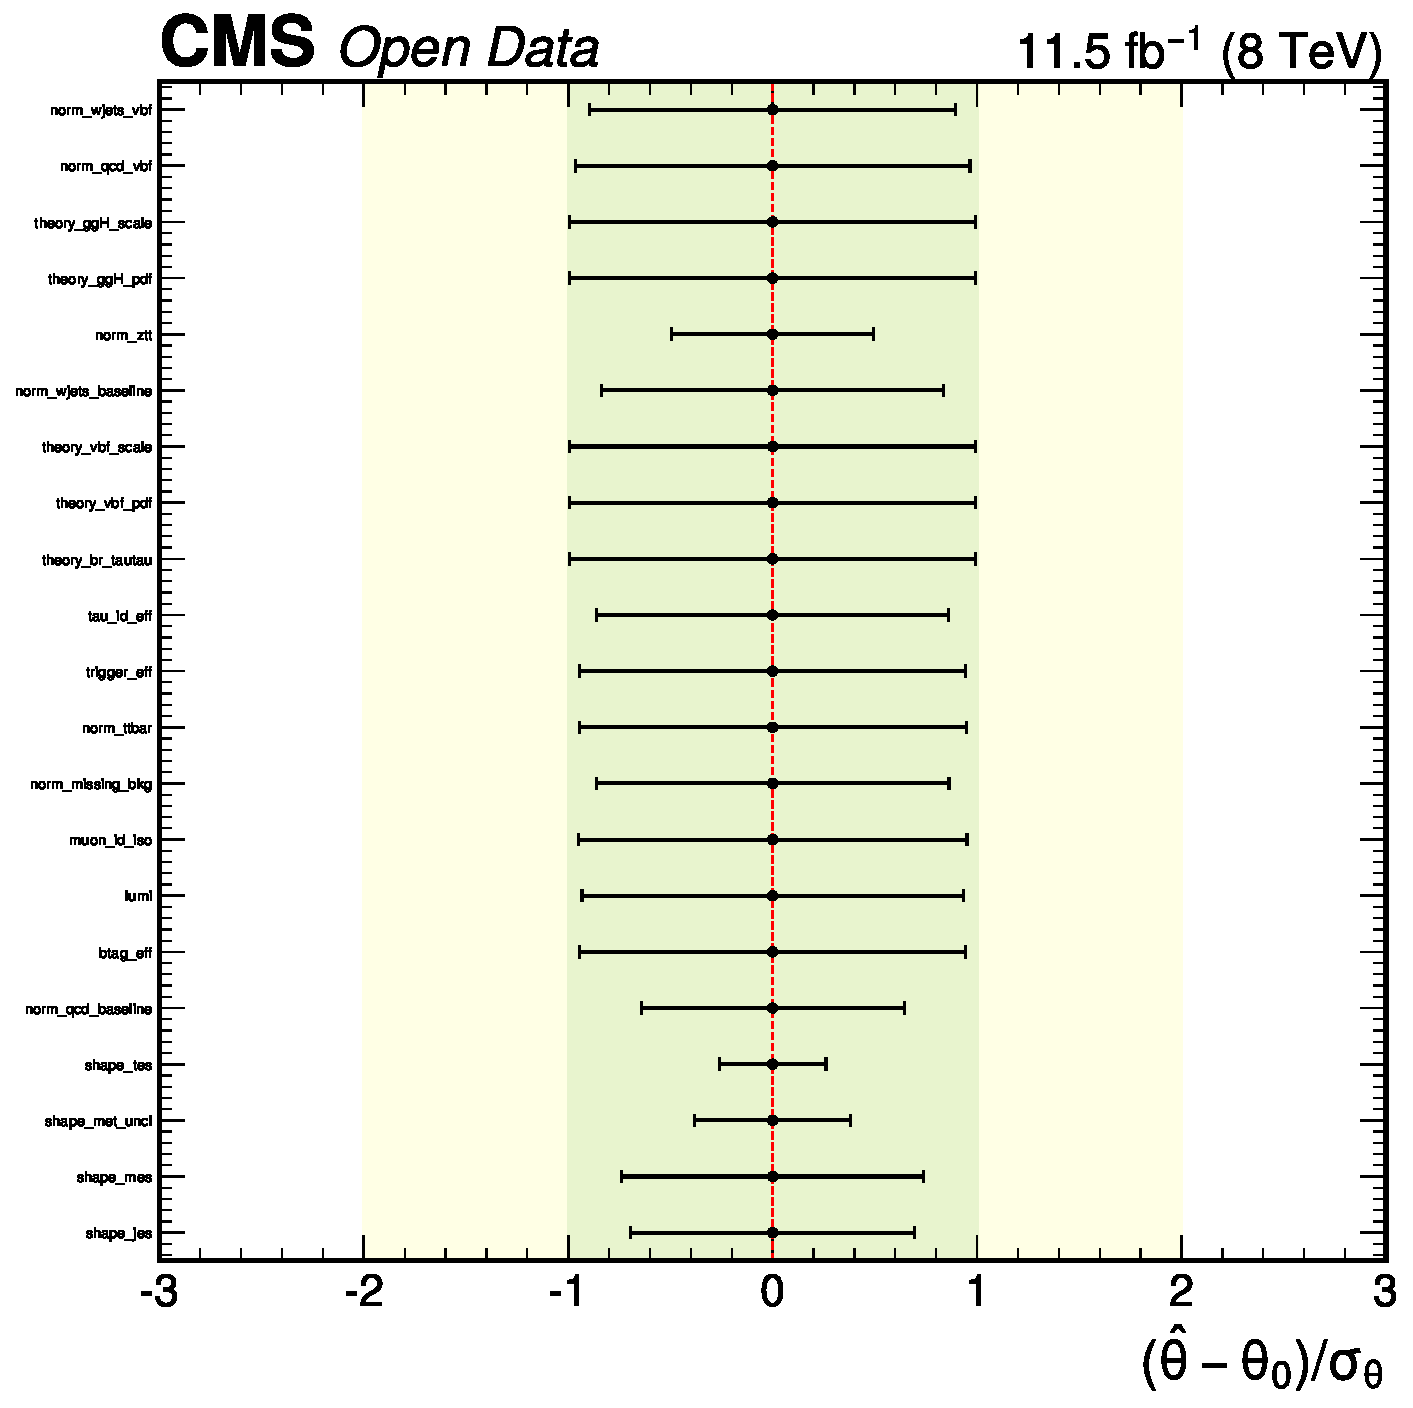
\includegraphics[height=0.35\textheight,width=\linewidth,keepaspectratio,alt={Nuisance parameter best-fit values and post-fit uncertainties for the NN score Asimov fit. The black points show the best-fit values (all zero on Asimov data) with error bars indicating the post-fit uncertainties. The green (yellow) bands show the 1\textbackslash sigma (2\textbackslash sigma) prior constraint regions. Several parameters, particularly the shape systematics (TES, MES, MET, JES), have post-fit uncertainties significantly smaller than the prior, indicating that the template shapes in the fit provide constraining information.}]{figures/np_pulls.pdf}}
\caption{Nuisance parameter best-fit values and post-fit uncertainties
for the NN score Asimov fit. The black points show the best-fit values
(all zero on Asimov data) with error bars indicating the post-fit
uncertainties. The green (yellow) bands show the 1\(\sigma\)
(2\(\sigma\)) prior constraint regions. Several parameters, particularly
the shape systematics (TES, MES, MET, JES), have post-fit uncertainties
significantly smaller than the prior, indicating that the template
shapes in the fit provide constraining information.}\label{fig:np-pulls}
\end{figure}

\needspace{4\baselineskip}
\subsection{Goodness of fit (Asimov)}\label{sec:val-gof}

The goodness of fit is assessed using a \(\chi^2\) statistic comparing
the fitted model prediction to the data. On Asimov data,
\(\chi^2 \approx 0\) by construction (the Asimov data is the model
prediction), confirming that the workspace is correctly assembled and
the fit converges.

The toy-based \(p\)-value is computed by generating 200
pseudo-experiments for the NN score approach and 100 each for
\(m_\mathrm{vis}\) and \(m_\mathrm{col}\). Since the Asimov
\(\chi^2 = 0\) is always less than any toy \(\chi^2\) (Figure~\ref{fig:gof-toys}), the \(p\)-value is 1.0 for all approaches.
This validates the toy generation and fitting machinery; the meaningful
goodness-of-fit test with informative \(p\)-values will occur on real
data.

The effective number of degrees of freedom is negative (\(-22\)) because
the model has more parameters (71) than data bins (50 for
\(m_\mathrm{vis}\)/25+25, 45 for NN/20+25). This is standard for
HistFactory models with many nuisance parameters; the GoF interpretation
relies on the toy-based \(p\)-value rather than the \(\chi^2\)/ndf
ratio.

\needspace{0.4\textheight}
\begin{figure}[htbp]
\centering
\pandocbounded{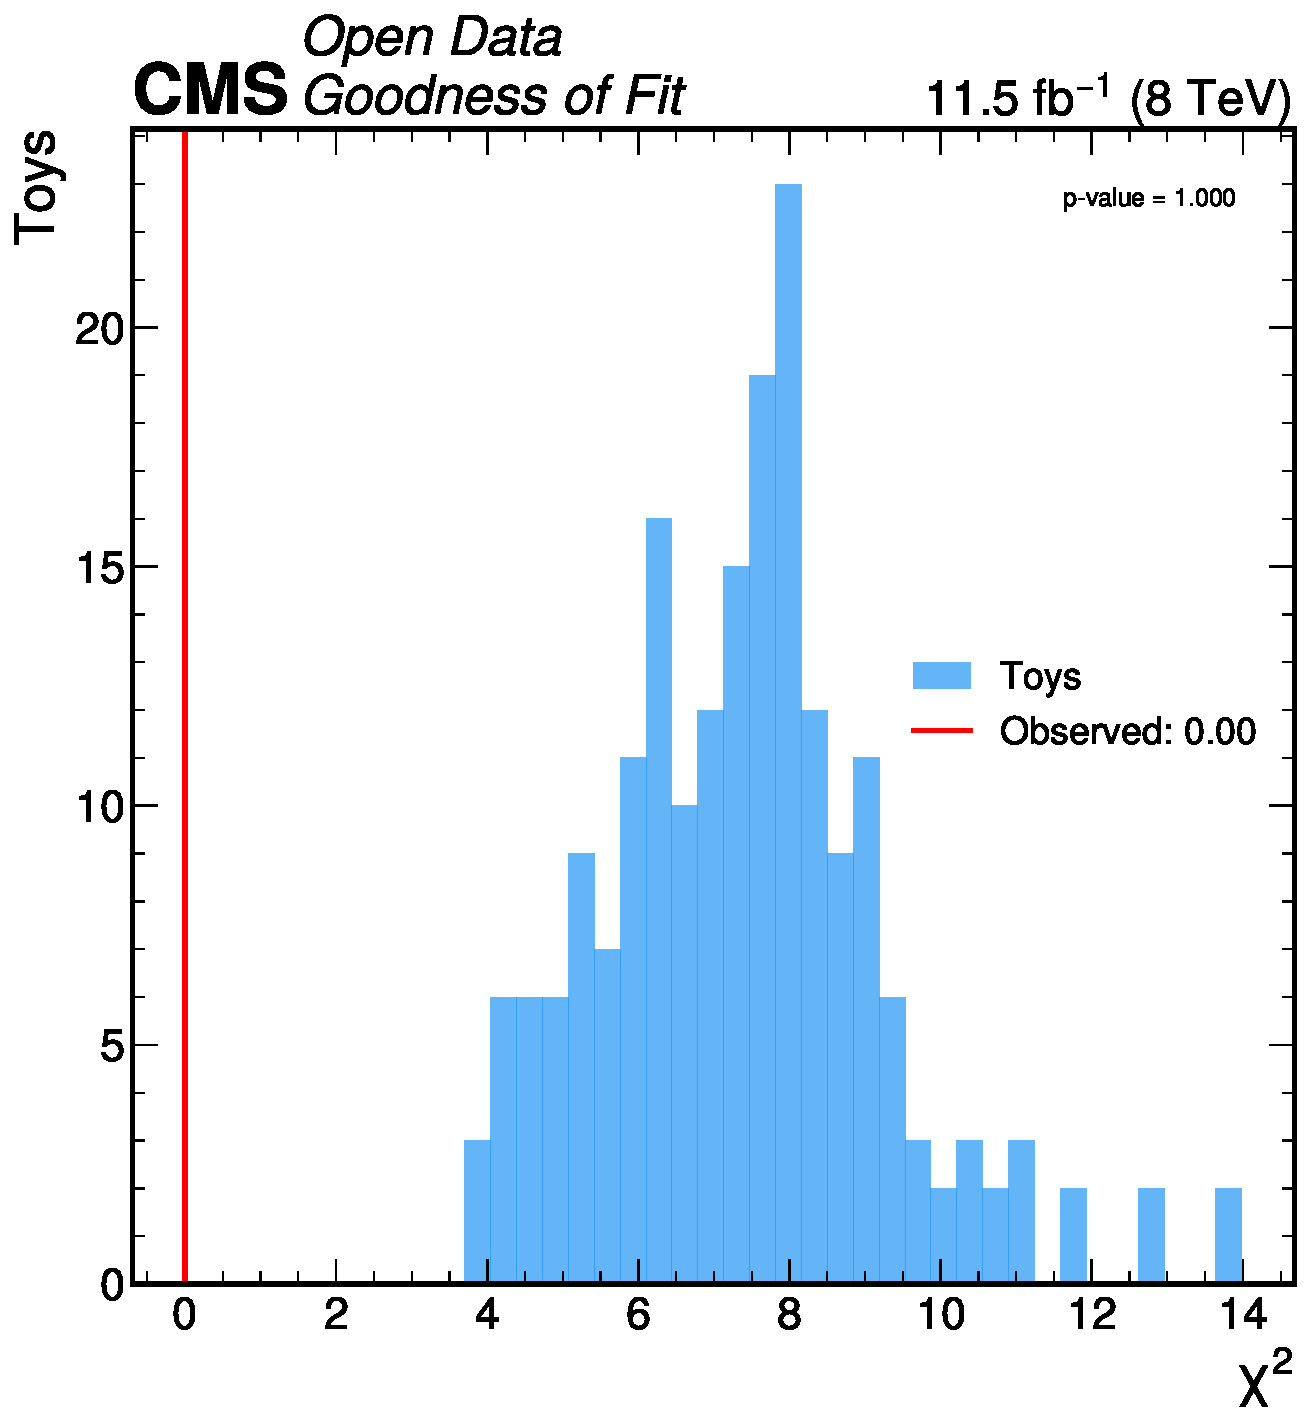
\includegraphics[height=0.35\textheight,width=\linewidth,keepaspectratio,alt={Distribution of \textbackslash chi\^{}2 values from 200 toy fits (blue histogram) compared to the Asimov observed \textbackslash chi\^{}2 \textbackslash approx 0 (red vertical line). All toy \textbackslash chi\^{}2 values exceed the Asimov value, yielding a p-value of 1.0. The toy \textbackslash chi\^{}2 distribution peaks near 6-7 with a tail extending to approximately 11, providing a reference for the expected GoF distribution when real data is fitted.}]{figures/gof_toys.pdf}}
\caption{Distribution of \(\chi^2\) values from 200 toy fits (blue
histogram) compared to the Asimov observed \(\chi^2 \approx 0\) (red
vertical line). All toy \(\chi^2\) values exceed the Asimov value,
yielding a \(p\)-value of 1.0. The toy \(\chi^2\) distribution peaks
near 6-7 with a tail extending to approximately 11, providing a
reference for the expected GoF distribution when real data is
fitted.}\label{fig:gof-toys}
\end{figure}

\needspace{4\baselineskip}
\subsection{Validation summary}\label{sec:val-summary}

Table~\ref{tbl:validation-summary} provides a comprehensive summary of
all validation tests performed and their outcomes.

\vspace{1em}
\begin{longtable}[]{@{}
  >{\raggedright\arraybackslash}p{(\linewidth - 8\tabcolsep) * \real{0.0896}}
  >{\raggedright\arraybackslash}p{(\linewidth - 8\tabcolsep) * \real{0.3284}}
  >{\raggedright\arraybackslash}p{(\linewidth - 8\tabcolsep) * \real{0.1642}}
  >{\raggedright\arraybackslash}p{(\linewidth - 8\tabcolsep) * \real{0.1343}}
  >{\raggedright\arraybackslash}p{(\linewidth - 8\tabcolsep) * \real{0.2836}}@{}}
\caption{Summary of all validation tests performed in this analysis,
including tests on Asimov pseudo-data, 10\% data validation, and full
observed data. All tests pass their respective criteria except the
full-data combined GoF, which is documented as a known limitation of the
MC modeling.}\label{tbl:validation-summary}\tabularnewline
\toprule\noalign{}
\begin{minipage}[b]{\linewidth}\raggedright
Test
\end{minipage} & \begin{minipage}[b]{\linewidth}\raggedright
\(\chi^2\)/ndf or metric
\end{minipage} & \begin{minipage}[b]{\linewidth}\raggedright
\(p\)-value
\end{minipage} & \begin{minipage}[b]{\linewidth}\raggedright
Verdict
\end{minipage} & \begin{minipage}[b]{\linewidth}\raggedright
What it validates
\end{minipage} \\
\midrule\noalign{}
\endfirsthead
\toprule\noalign{}
\begin{minipage}[b]{\linewidth}\raggedright
Test
\end{minipage} & \begin{minipage}[b]{\linewidth}\raggedright
\(\chi^2\)/ndf or metric
\end{minipage} & \begin{minipage}[b]{\linewidth}\raggedright
\(p\)-value
\end{minipage} & \begin{minipage}[b]{\linewidth}\raggedright
Verdict
\end{minipage} & \begin{minipage}[b]{\linewidth}\raggedright
What it validates
\end{minipage} \\
\midrule\noalign{}
\endhead
\bottomrule\noalign{}
\endlastfoot
NN AUC (test) & 0.825 & N/A & GO (\textgreater{} 0.75 threshold) &
Discriminant quality \\
NN overtraining (signal) & KS = 0.028 & 0.127 & PASS (\(p > 0.05\)) & No
overtraining \\
NN overtraining (bkg) & KS = 0.008 & 0.686 & PASS (\(p > 0.05\)) & No
overtraining \\
BDT comparison & AUC = 0.820 & N/A & Consistent & Architecture
robustness \\
Signal injection (\(\mu=0\), NN) & Pull = 0.000 & N/A & PASS
(\(|\)pull\(|\) \textless{} 0.1) & Workspace sanity check \\
Signal injection (\(\mu=1\), NN) & Pull = 0.000 & N/A & PASS
(\(|\)pull\(|\) \textless{} 0.1) & Workspace sanity check \\
Signal injection (\(\mu=2\), NN) & Pull = \(-0.002\) & N/A & PASS
(\(|\)pull\(|\) \textless{} 0.1) & Fit linearity \\
Signal injection (\(\mu=5\), NN) & Pull = 0.000 & N/A & PASS
(\(|\)pull\(|\) \textless{} 0.1) & Fit linearity at high \(\mu\) \\
NP pulls (Asimov, NN) & All pulls = 0 & N/A & PASS & Workspace
assembly \\
GoF (Asimov, NN) & \(\chi^2 \approx 0\) & 1.0 (200 toys) & Expected &
Toy machinery \\
GoF (Asimov, \(m_\mathrm{vis}\)) & \(\chi^2 \approx 0\) & 1.0 (100 toys)
& Expected & Toy machinery \\
GoF (Asimov, \(m_\mathrm{col}\)) & \(\chi^2 \approx 0\) & 1.0 (99 toys)
& Expected & Toy machinery \\
Tau ID WP optimization & \(\chi^2\)/ndf = 2.96 (Loose) & N/A & Selected
& Data/MC modeling \\
\(W\)+jets SF & 0.999 ± 0.008 & N/A & Consistent with 1 & Background
normalization \\
\(W\)+jets validation (mid-\(m_\mathrm{T}\)) & Data/Pred = 1.087 & N/A &
Consistent (QCD) & Normalization extrapolation \\
QCD OS/SS ratio & 0.979 ± 0.018 & N/A & Within range & QCD estimation
method \\
Collinear mass go/no-go & 45.7\% unphysical (ggH) & N/A & GO
(\textless{} 50\%) & Observable viability \\
10\% NP pulls (NN) & Max = \(-1.85\sigma\) & N/A & PASS (\textless{}
2\(\sigma\)) & No systematic mismodeling \\
10\% GoF (NN) & \(\chi^2 = 34.4\) & 0.209 & PASS (\(p > 0.05\)) & Model
describes 10\% data \\
10\% \(\hat{\mu}\) pull (NN) & \(-1.69\sigma\) & N/A & PASS (\textless{}
2\(\sigma\)) & Framework on real data \\
Full data NP pulls (NN) & Max = \(-1.89\sigma\) & N/A & PASS
(\textless{} 2\(\sigma\)) & Post-fit NP behavior \\
Full data GoF (NN) & \(\chi^2 = 33.1\) & 0.000 & FLAG (documented) &
Known MC limitation \\
Full data per-cat \(\chi^2\)/bin (NN) & 0.86 / 0.80 & N/A & PASS
(\textless{} 1.5) & Per-category modeling \\
Per-cat \(\mu\) consistency (NN) & 0.61 vs \(-0.04\) & N/A & PASS
(\textless{} 1\(\sigma\) apart) & Category consistency \\
Published comparison & Pull = \(-0.13\sigma\) & N/A & PASS & External
consistency \\
\end{longtable}

\needspace{4\baselineskip}
\FloatBarrier
\section{10\% Data Validation}\label{sec:data-validation}

This section presents the results of a 10\% data validation, in which a
random subsample of the collision data is compared to the MC prediction
and fitted to extract the signal strength. The purpose of this
validation is to confirm that the analysis framework --- workspace
construction, fitting procedure, systematic treatment, and
goodness-of-fit evaluation --- functions correctly on real data before
proceeding to unblind the full dataset.

\needspace{4\baselineskip}
\subsection{Data subsample selection}\label{sec:10pct-selection}

A 10\% random subsample of the observed data is selected using
\texttt{np.random.RandomState(seed=42)}. The same random mask is applied
consistently to the main arrays, NN scores, and collinear mass arrays
for both OS and SS signal regions.

\vspace{1em}
\begin{table}[htbp]
\centering
\small
\caption{Summary of the 10\% data subsample selection. The subsample
fractions are consistent with 10\% within Poisson statistics (expected
fluctuations of order 0.3\%).}\label{tbl:10pct-selection}
\begin{tabular}{@{}
>{\raggedright\arraybackslash}p{(\linewidth - 12\tabcolsep) * \real{0.1233}}
  >{\raggedright\arraybackslash}p{(\linewidth - 12\tabcolsep) * \real{0.1507}}
  >{\raggedright\arraybackslash}p{(\linewidth - 12\tabcolsep) * \real{0.1507}}
  >{\raggedright\arraybackslash}p{(\linewidth - 12\tabcolsep) * \real{0.1370}}
  >{\raggedright\arraybackslash}p{(\linewidth - 12\tabcolsep) * \real{0.1507}}
  >{\raggedright\arraybackslash}p{(\linewidth - 12\tabcolsep) * \real{0.1507}}
  >{\raggedright\arraybackslash}p{(\linewidth - 12\tabcolsep) * \real{0.1370}}@{}}
\toprule\noalign{}
\begin{minipage}[b]{\linewidth}\raggedright
Dataset
\end{minipage} & \begin{minipage}[b]{\linewidth}\raggedright
OS SR full
\end{minipage} & \begin{minipage}[b]{\linewidth}\raggedright
OS SR 10\%
\end{minipage} & \begin{minipage}[b]{\linewidth}\raggedright
Fraction
\end{minipage} & \begin{minipage}[b]{\linewidth}\raggedright
SS SR full
\end{minipage} & \begin{minipage}[b]{\linewidth}\raggedright
SS SR 10\%
\end{minipage} & \begin{minipage}[b]{\linewidth}\raggedright
Fraction
\end{minipage} \\
\midrule\noalign{}
\toprule\noalign{}
\begin{minipage}[b]{\linewidth}\raggedright
Dataset
\end{minipage} & \begin{minipage}[b]{\linewidth}\raggedright
OS SR full
\end{minipage} & \begin{minipage}[b]{\linewidth}\raggedright
OS SR 10\%
\end{minipage} & \begin{minipage}[b]{\linewidth}\raggedright
Fraction
\end{minipage} & \begin{minipage}[b]{\linewidth}\raggedright
SS SR full
\end{minipage} & \begin{minipage}[b]{\linewidth}\raggedright
SS SR 10\%
\end{minipage} & \begin{minipage}[b]{\linewidth}\raggedright
Fraction
\end{minipage} \\
\midrule\noalign{}
\bottomrule\noalign{}
Run2012B & 26,236 & 2,646 & 10.09\% & 8,879 & 876 & 9.87\% \\
Run2012C & 41,752 & 4,175 & 10.00\% & 14,255 & 1,427 & 10.01\% \\
\textbf{Total} & \textbf{67,988} & \textbf{6,821} & \textbf{10.03\%} &
\textbf{23,134} & \textbf{2,303} & \textbf{9.96\%} \\
\end{tabular}
\end{table}

\needspace{4\baselineskip}
\subsection{Data/MC comparison (pre-fit)}\label{sec:10pct-datamc}

The 10\% data histograms are scaled by 10 for comparison to the full MC
prediction from the expected-results study. The MC templates are
unchanged (full MC statistics retained for all processes).

\subsubsection{Total yields}\label{sec:10pct-yields}

\vspace{1em}
\begin{table}[htbp]
\centering
\small
\caption{Data/MC yield comparison for the 10\% subsample (scaled by 10)
in both categories across all three fitting approaches. The Baseline
category shows a 5\% deficit consistent with statistical fluctuations,
while the VBF category shows a 33-35\% deficit driven by the low
statistics of the 10\%
subsample.}\label{tbl:10pct-yields}
\begin{tabular}{@{}
llllll@{}}
\toprule\noalign{}
Approach & Category & Data (10\% x10) & MC expected & Ratio & Deficit \\
\midrule\noalign{}
\bottomrule\noalign{}
\(m_\mathrm{vis}\) & Baseline & 67,150 & 70,677 & 0.950 & 5.0\% \\
\(m_\mathrm{vis}\) & VBF & 820 & 1,235 & 0.664 & 33.6\% \\
NN score & Baseline & 67,390 & 70,898 & 0.951 & 4.9\% \\
NN score & VBF & 820 & 1,260 & 0.651 & 34.9\% \\
\(m_\mathrm{col}\) & Baseline & 59,250 & 62,695 & 0.945 & 5.5\% \\
\(m_\mathrm{col}\) & VBF & 800 & 1,185 & 0.675 & 32.5\% \\
\end{tabular}
\end{table}

\textbf{Baseline category:} The 5\% deficit is consistent with
statistical fluctuations in a 10\% subsample. The expected statistical
uncertainty on the total yield is
\(\sqrt{N_\mathrm{10\%}} / N_\mathrm{10\%} \times 10 = 10/\sqrt{N_\mathrm{10\%}}\),
which for approximately 6,800 events gives approximately 12\%, well
larger than the 5\% observed deficit.

\textbf{VBF category:} The 33-35\% deficit is a notable feature. With
only approximately 82 observed events in 10\% of the data (expected
approximately 126 if the full dataset matches MC), the deficit
corresponds to a Poisson fluctuation of
\((126 - 82)/\sqrt{82} \approx 4.9\). However, the VBF category has only
approximately 800 total events across both run periods, making it highly
susceptible to statistical fluctuations in a 10\% subsample. The full
dataset will determine whether this deficit persists.

\subsubsection{Data/MC distributions}\label{sec:10pct-distributions}

Figures~\ref{fig:10pct-mvis-baseline}--Figure~\ref{fig:10pct-mcol-vbf} show
the data/MC comparisons for all three discriminant variables in both
categories.

\needspace{0.4\textheight}
\begin{figure}[htbp]
\centering
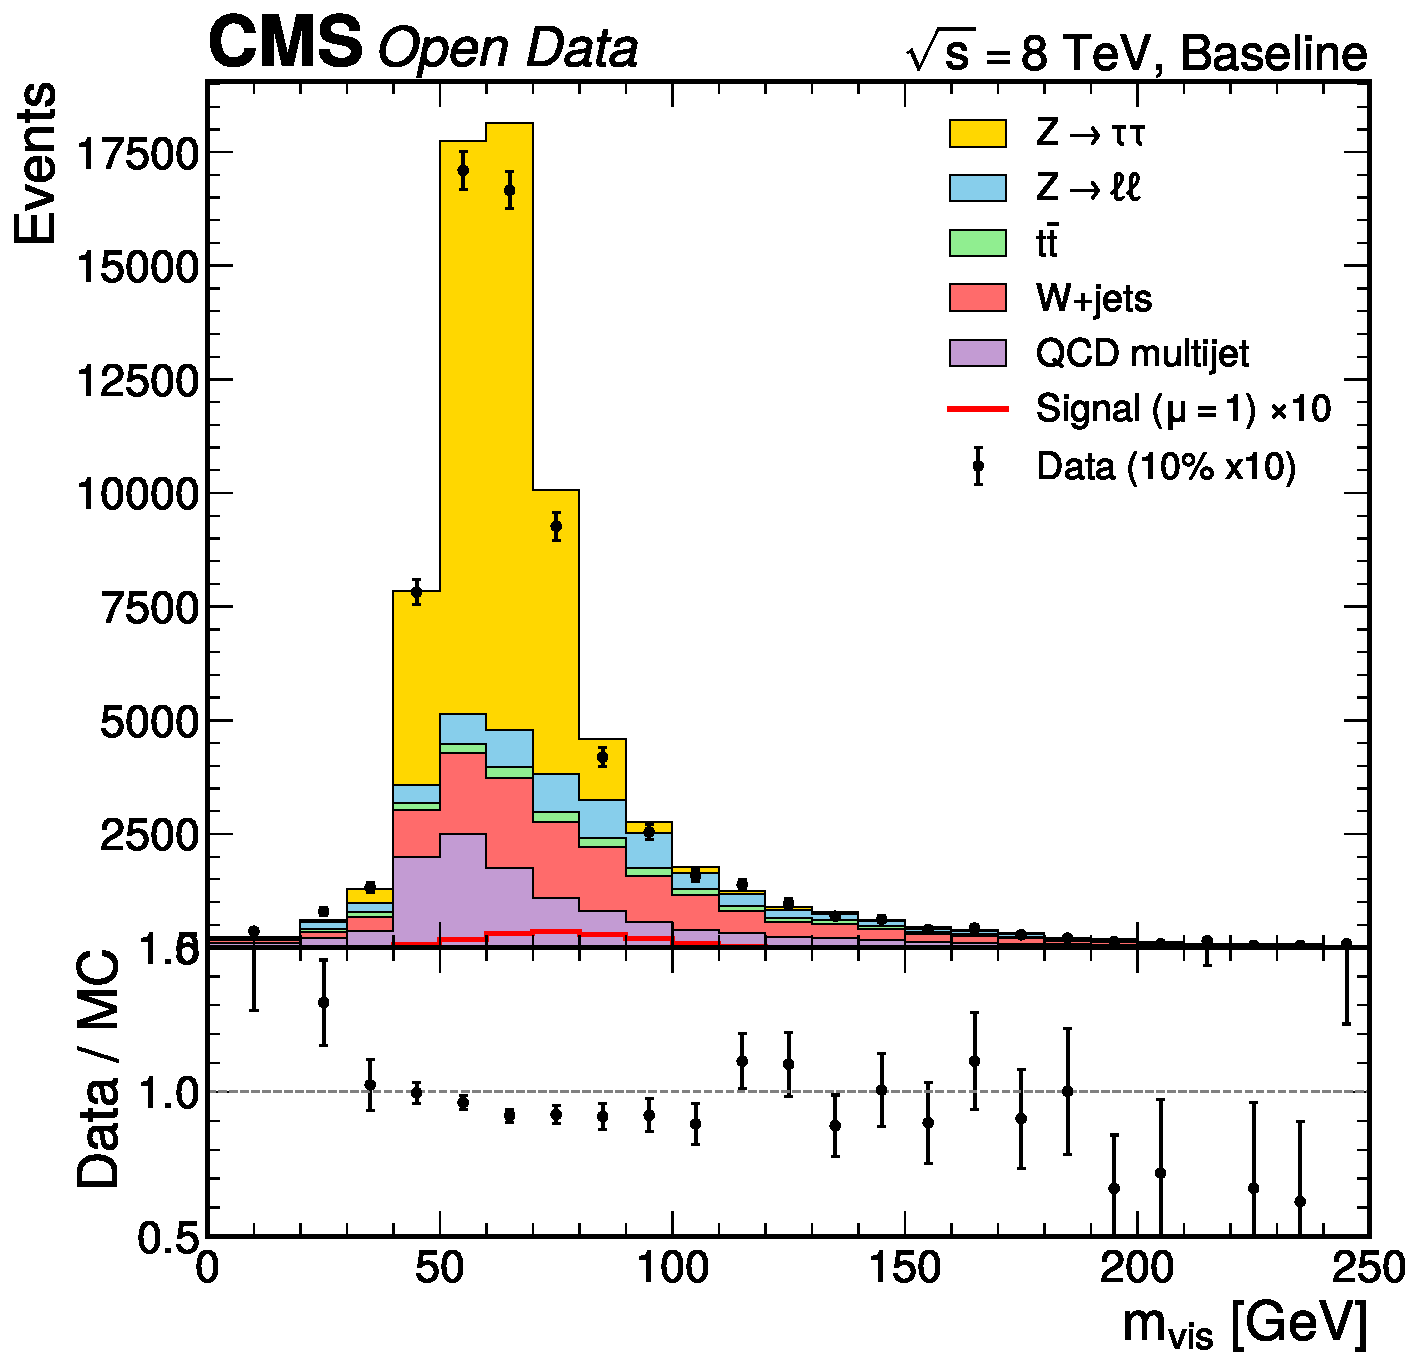
\includegraphics[height=0.38\linewidth,keepaspectratio]{figures/data_mc_mvis_baseline.pdf}\hspace{0.02\linewidth}
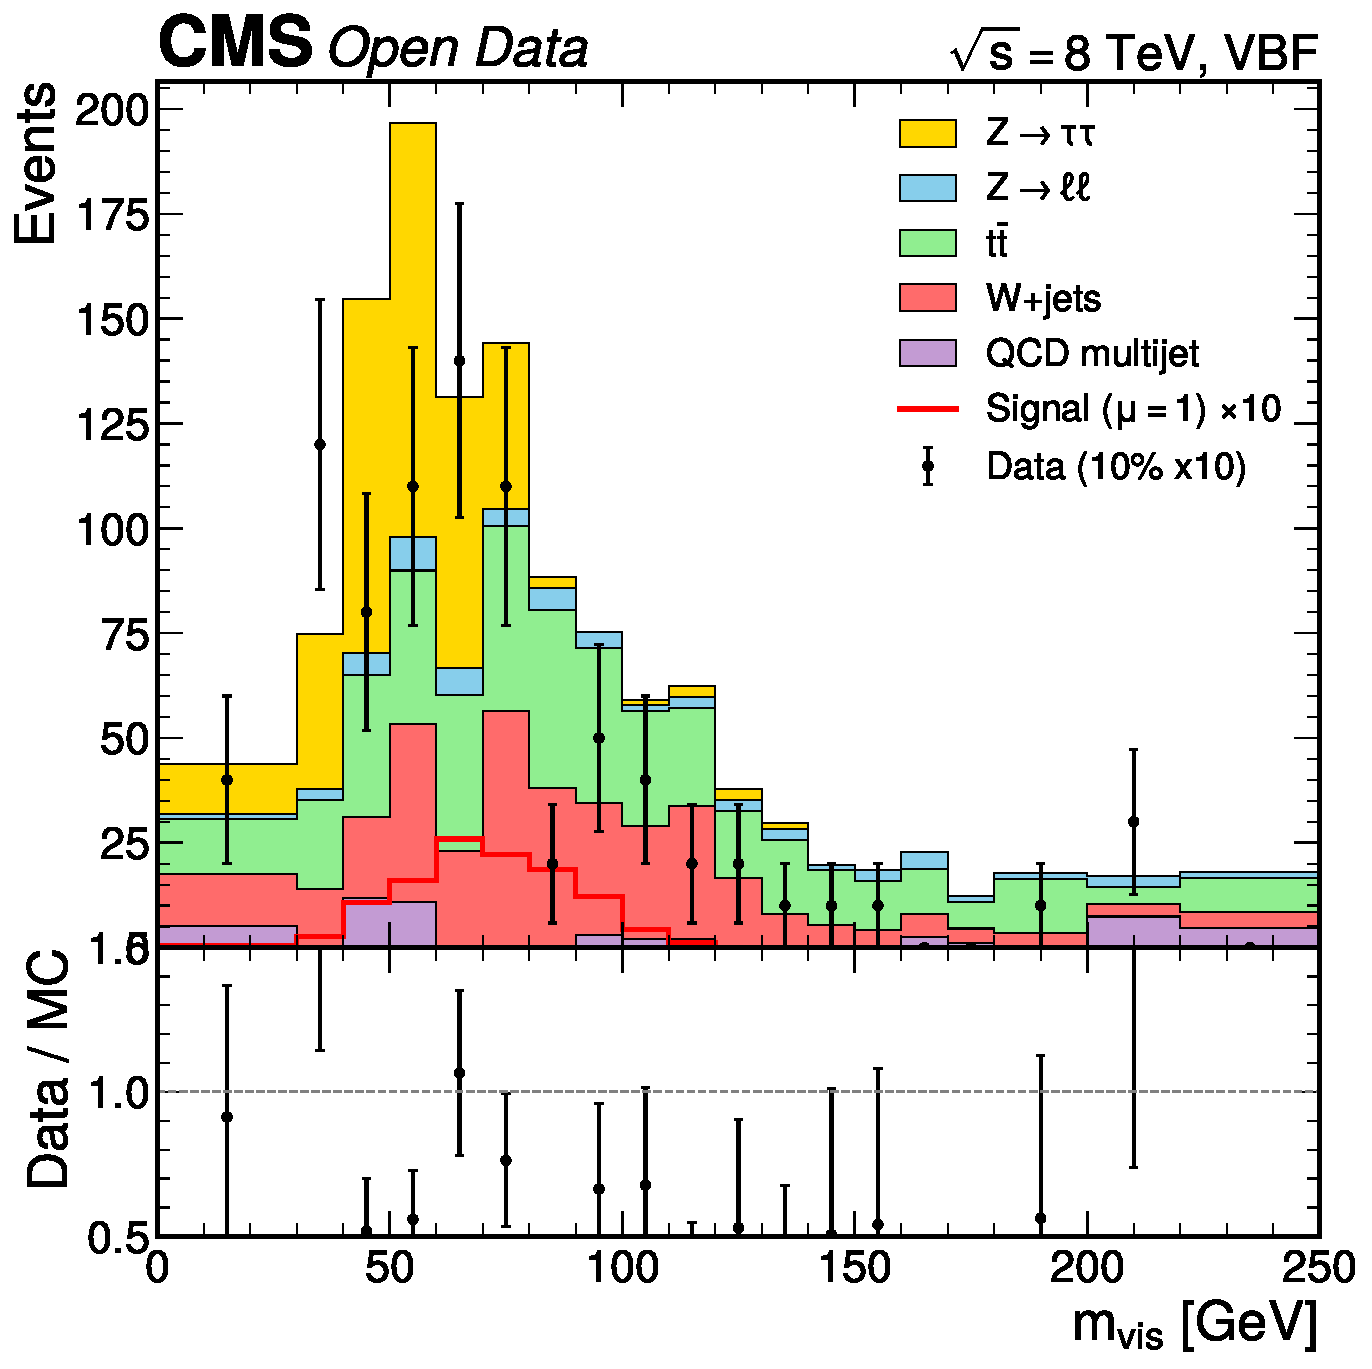
\includegraphics[height=0.38\linewidth,keepaspectratio]{figures/data_mc_mvis_vbf.pdf}
\caption{(a) Visible mass data/MC comparison in the Baseline category using
the 10\% data subsample (scaled by 10). The stacked MC prediction from
the expected-results study is overlaid with the 10\% data points. The
data/MC ratio of 0.95 is consistent with statistical fluctuations. The
shape agreement is good across the full \(m_\mathrm{vis}\) range, with
no significant distortions in the \(Z\) peak or Higgs signal
regions. (b) Visible mass data/MC comparison in the VBF category. The 10\%
data deficit of 34\% is visible across the full mass range, with the
most prominent deficit in the 60-120 GeV region corresponding to the
\(Z\to\tau\tau\) peak. The deficit is consistent with a statistical
fluctuation given the small event count (82 events in
10\%).}\label{fig:10pct-mvis-baseline}
\phantomsection\label{fig:10pct-mvis-vbf}
\end{figure}


\needspace{0.4\textheight}
\begin{figure}[htbp]
\centering
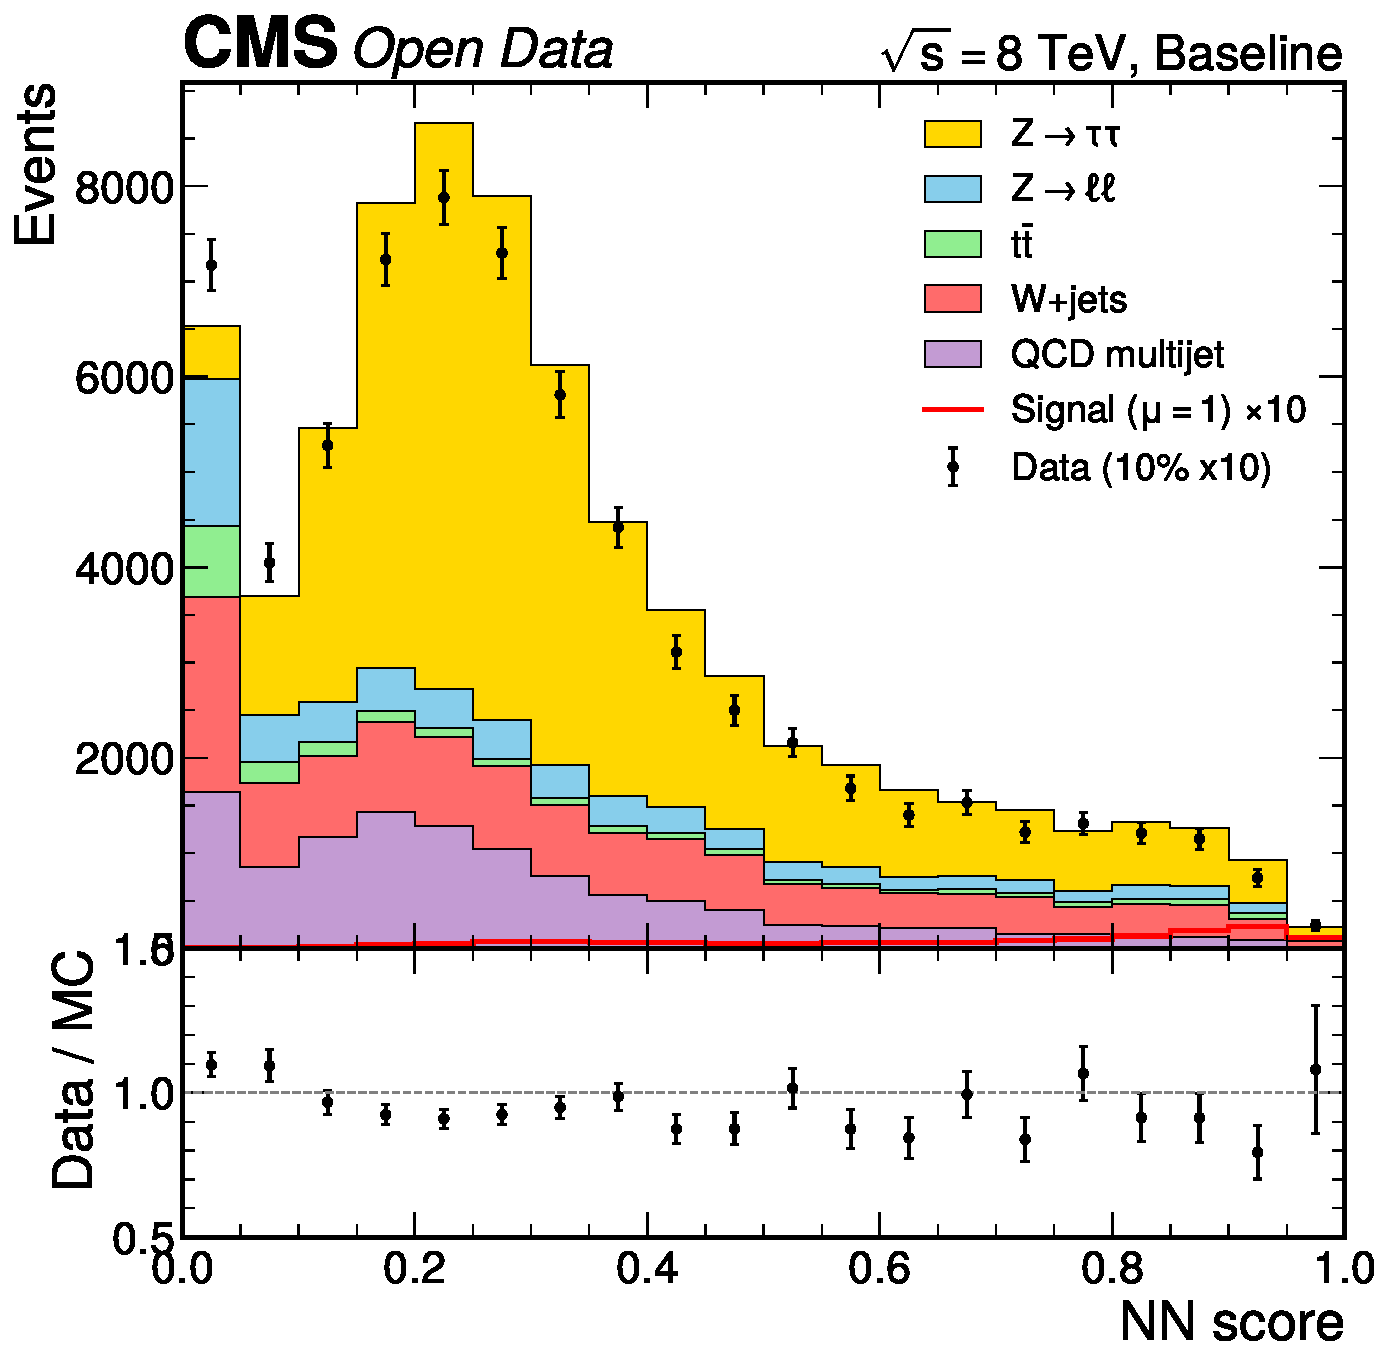
\includegraphics[height=0.38\linewidth,keepaspectratio]{figures/data_mc_nn_score_baseline.pdf}\hspace{0.02\linewidth}
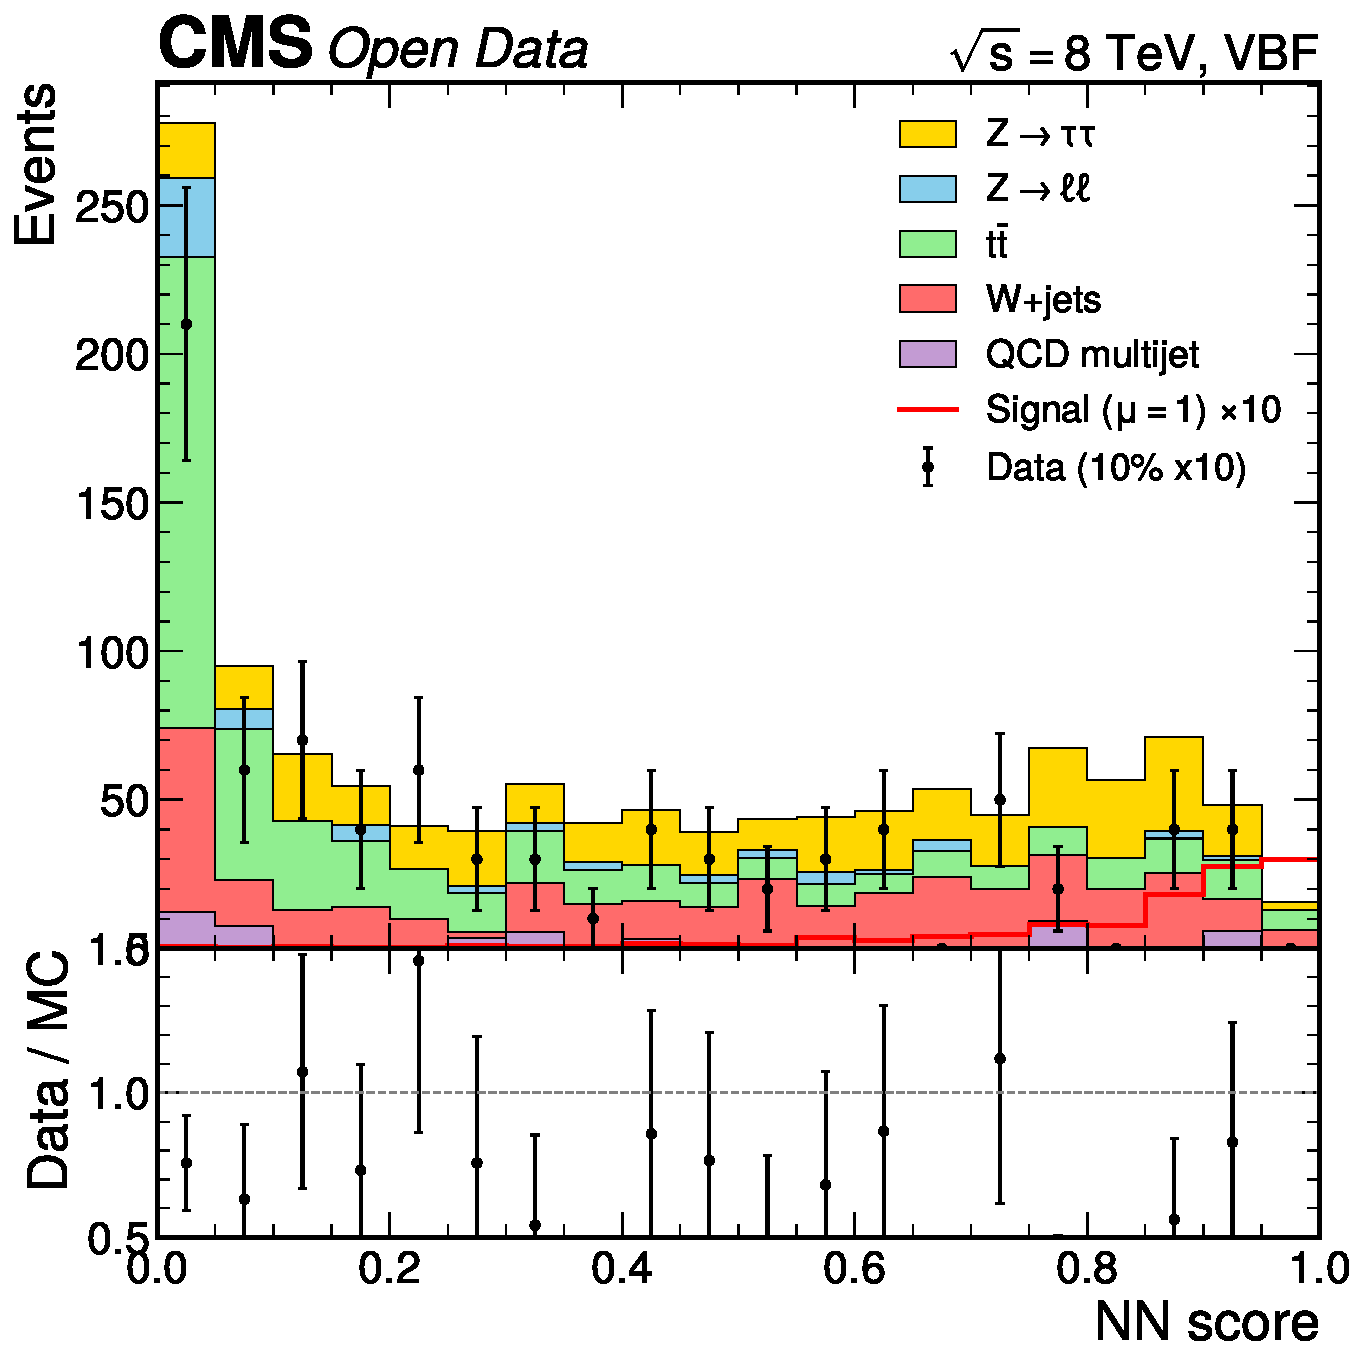
\includegraphics[height=0.38\linewidth,keepaspectratio]{figures/data_mc_nn_score_vbf.pdf}
\caption{(a) NN discriminant score data/MC comparison in the Baseline
category using the 10\% data subsample. The data follows the MC
prediction within statistical uncertainties across the full NN score
range, from the background-dominated low-score region to the
signal-enriched high-score region. Data/MC ratio is 0.95, consistent
with the Baseline yield deficit. (b) NN discriminant score data/MC comparison in the VBF category.
The 10\% data deficit is visible across all NN score bins. The reduced
statistics in the VBF category lead to large fluctuations in the ratio
panel. The deficit does not appear to be concentrated in any particular
NN score region, suggesting an overall normalization effect rather than
a shape mismodeling.}\label{fig:10pct-nn-baseline}
\phantomsection\label{fig:10pct-nn-vbf}
\end{figure}


\needspace{0.4\textheight}
\begin{figure}[htbp]
\centering
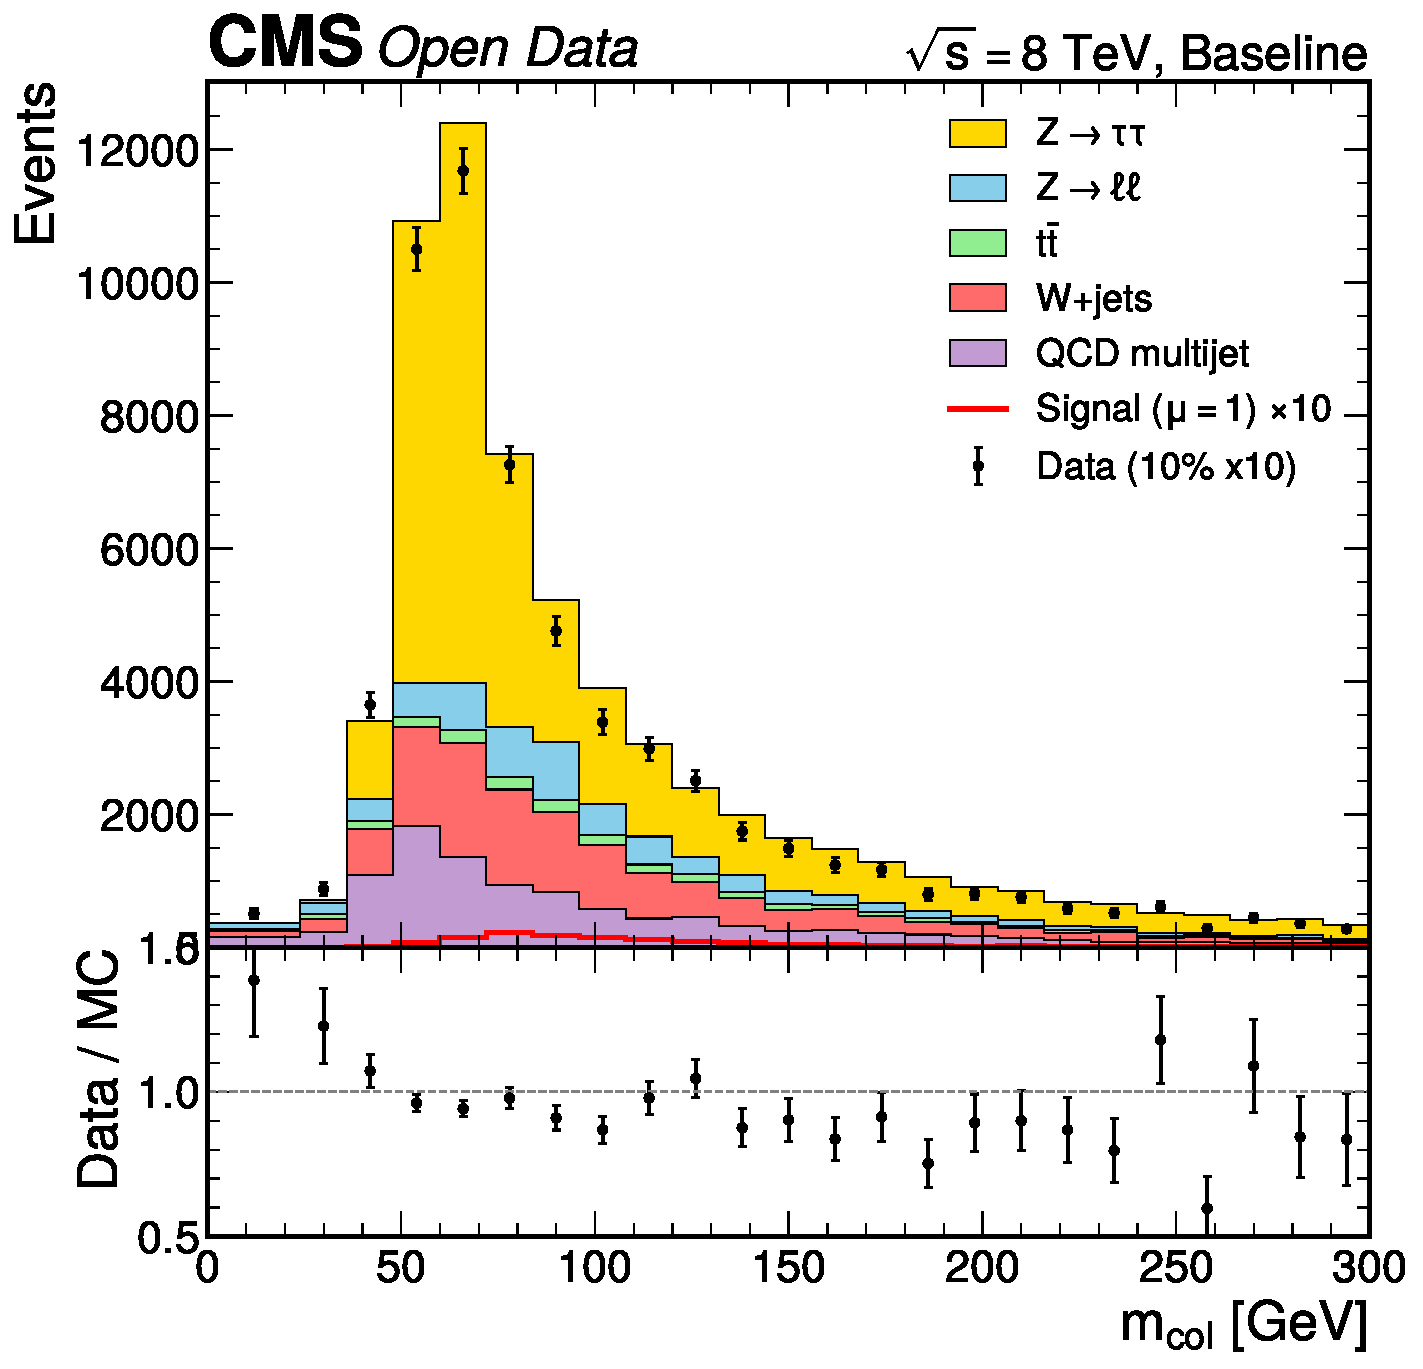
\includegraphics[height=0.38\linewidth,keepaspectratio]{figures/data_mc_mcol_baseline.pdf}\hspace{0.02\linewidth}
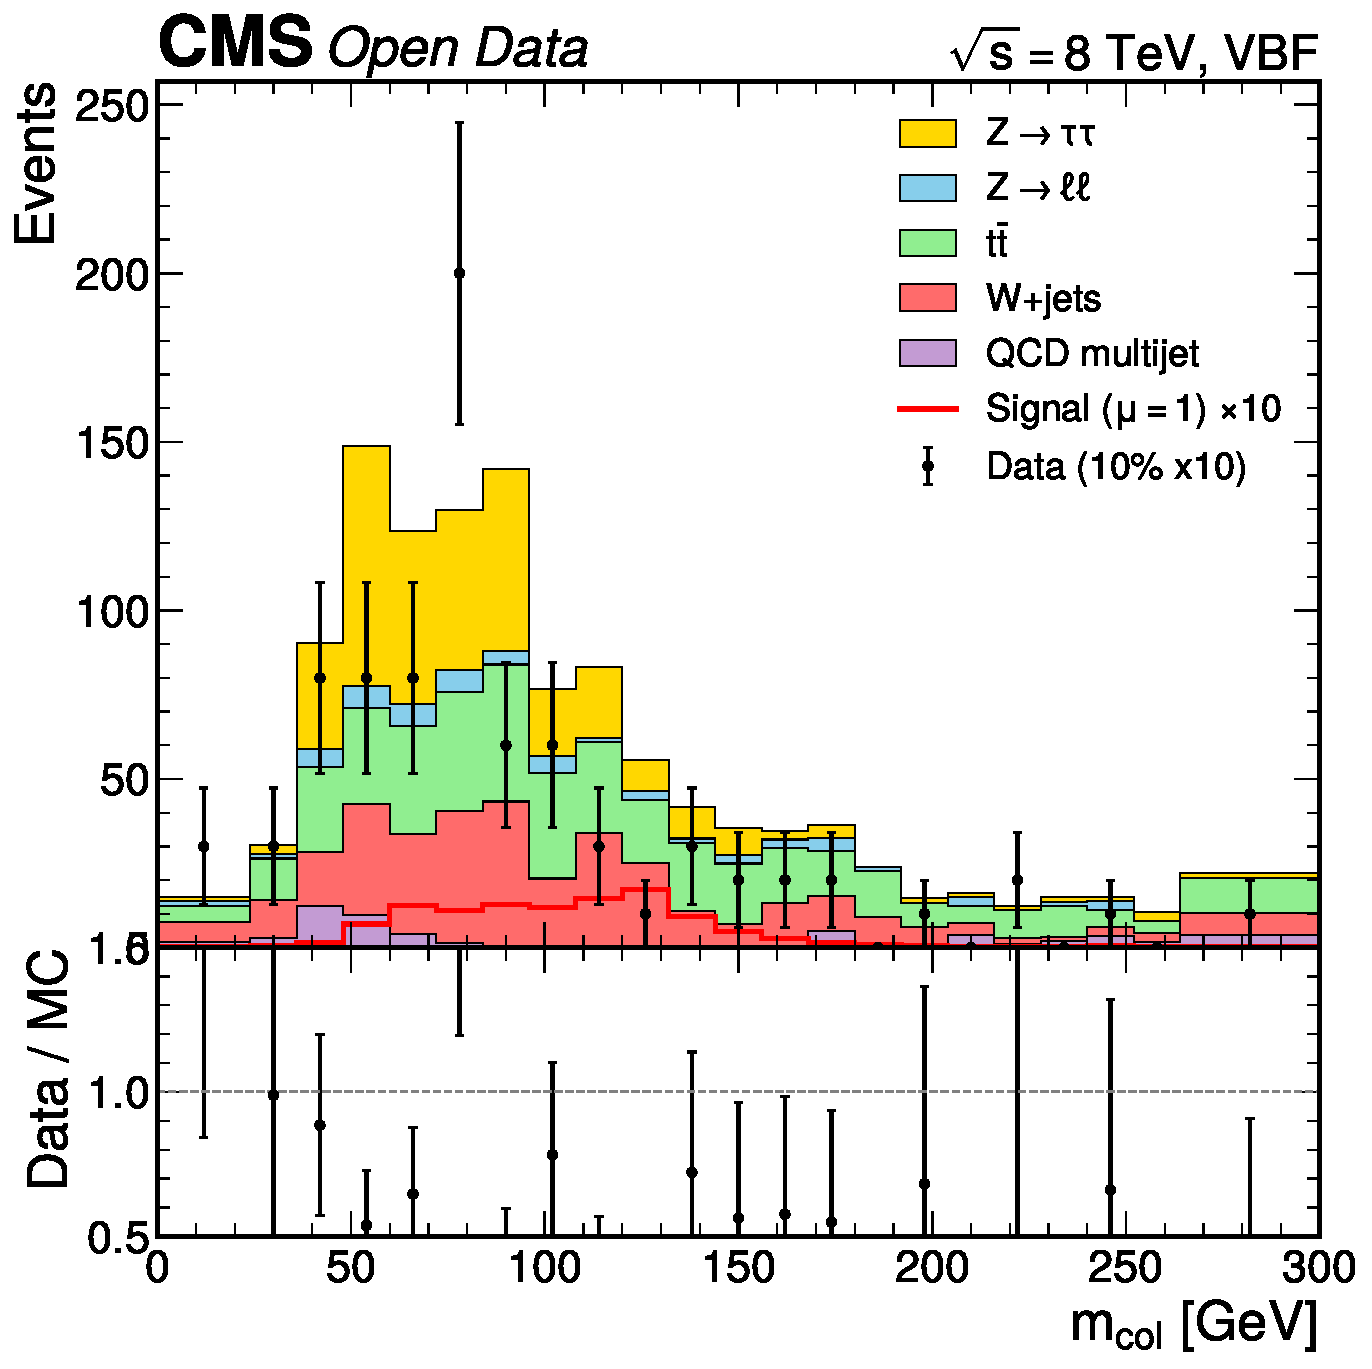
\includegraphics[height=0.38\linewidth,keepaspectratio]{figures/data_mc_mcol_vbf.pdf}
\caption{(a) Collinear mass data/MC comparison in the Baseline category. The
data/MC agreement is comparable to the visible mass approach, with a
5.5\% overall deficit. The broader distribution due to unphysical
collinear solutions is reproduced by the MC
prediction. (b) Collinear mass data/MC comparison in the VBF category. The 33\%
deficit is visible, consistent with the other approaches. The collinear
mass distribution shows larger bin-to-bin fluctuations due to the
combination of low statistics and the unphysical solution
fallback.}\label{fig:10pct-mcol-baseline}
\phantomsection\label{fig:10pct-mcol-vbf}
\end{figure}


\subsubsection{QCD template from 10\% data}\label{sec:10pct-qcd}

The QCD template is estimated from the 10\% SS data:
\(N_\mathrm{QCD,10\%} = (N_\mathrm{data,SS,10\%} - N_\mathrm{MC,SS} \times 0.1) \times R_\mathrm{OS/SS}\).

\vspace{1em}
\begin{table}[htbp]
\centering
\small
\caption{Comparison of the QCD background estimate from the 10\% data
versus the full dataset (the expected-results study). The Baseline QCD
agrees within 1\%. The VBF QCD shows a factor of approximately 2 excess,
driven by Poisson fluctuations in the very small SS VBF sample
(approximately 5 events in 10\% after MC
subtraction).}\label{tbl:10pct-qcd}
\begin{tabular}{@{}
lllll@{}}
\toprule\noalign{}
Approach & Category & QCD (10\% x10) & QCD (Asimov) & Ratio \\
\midrule\noalign{}
\bottomrule\noalign{}
\(m_\mathrm{vis}\) & Baseline & 11,063 & 11,168 & 0.991 \\
\(m_\mathrm{vis}\) & VBF & 120 & 51 & 2.37 \\
NN score & Baseline & 11,072 & 11,197 & 0.989 \\
NN score & VBF & 119 & 47 & 2.53 \\
\(m_\mathrm{col}\) & Baseline & 10,065 & 10,013 & 1.005 \\
\(m_\mathrm{col}\) & VBF & 107 & 52 & 2.04 \\
\end{tabular}
\end{table}

The QCD estimate in the Baseline category agrees within 1\% with the
full estimate, confirming the stability of the data-driven QCD
estimation procedure. The VBF QCD shows a factor of approximately 2
excess, but this involves very small numbers (approximately 5 events in
10\% SS VBF, after MC subtraction) and is dominated by Poisson
fluctuations.

\needspace{4\baselineskip}
\subsection{Signal strength results on 10\% data}\label{sec:10pct-fit}

\subsubsection{Fitting methodology}\label{sec:10pct-fit-method}

The pyhf workspaces from the expected-results study are modified by
scaling all MC templates (nominal, shape systematics, staterror) by 0.1,
while the raw 10\% data (unscaled integers) serves as the observed data.
This preserves the Poisson nature of the data and avoids artifacts from
non-integer observations.

\subsubsection{Fitted signal strengths}\label{sec:10pct-mu}

Table~\ref{tbl:10pct-mu-results} compares the 10\% data fit results with
the expected (Asimov) results from the expected-results study.

\vspace{1em}
\begin{table}[htbp]
\centering
\small
\caption{Comparison of signal strength results from the 10\% data fit
and the Asimov expectation. The NN score pull of \(-1.69\sigma\) is
within the 2\(\sigma\) threshold. With extended POI bounds {[}-30,
30{]}, all approaches converge freely without hitting a
boundary.}\label{tbl:10pct-mu-results}
\begin{tabular}{@{}
>{\raggedright\arraybackslash}p{(\linewidth - 10\tabcolsep) * \real{0.0926}}
  >{\raggedright\arraybackslash}p{(\linewidth - 10\tabcolsep) * \real{0.1759}}
  >{\raggedright\arraybackslash}p{(\linewidth - 10\tabcolsep) * \real{0.1852}}
  >{\raggedright\arraybackslash}p{(\linewidth - 10\tabcolsep) * \real{0.1296}}
  >{\raggedright\arraybackslash}p{(\linewidth - 10\tabcolsep) * \real{0.2130}}
  >{\raggedright\arraybackslash}p{(\linewidth - 10\tabcolsep) * \real{0.2037}}@{}}
\toprule\noalign{}
\begin{minipage}[b]{\linewidth}\raggedright
Approach
\end{minipage} & \begin{minipage}[b]{\linewidth}\raggedright
\(\hat{\mu}\) (10\%)
\end{minipage} & \begin{minipage}[b]{\linewidth}\raggedright
\(\sigma(\mu)\) (10\%)
\end{minipage} & \begin{minipage}[b]{\linewidth}\raggedright
Pull from SM
\end{minipage} & \begin{minipage}[b]{\linewidth}\raggedright
\(\hat{\mu}\) (Asimov)
\end{minipage} & \begin{minipage}[b]{\linewidth}\raggedright
\(\sigma(\mu)\) (Asimov)
\end{minipage} \\
\midrule\noalign{}
\toprule\noalign{}
\begin{minipage}[b]{\linewidth}\raggedright
Approach
\end{minipage} & \begin{minipage}[b]{\linewidth}\raggedright
\(\hat{\mu}\) (10\%)
\end{minipage} & \begin{minipage}[b]{\linewidth}\raggedright
\(\sigma(\mu)\) (10\%)
\end{minipage} & \begin{minipage}[b]{\linewidth}\raggedright
Pull from SM
\end{minipage} & \begin{minipage}[b]{\linewidth}\raggedright
\(\hat{\mu}\) (Asimov)
\end{minipage} & \begin{minipage}[b]{\linewidth}\raggedright
\(\sigma(\mu)\) (Asimov)
\end{minipage} \\
\midrule\noalign{}
\bottomrule\noalign{}
\(m_\mathrm{vis}\) & \(-14.44\) & 5.94 & \(-2.60\sigma\) & 1.000 &
3.083 \\
\textbf{NN score} & \textbf{\(-3.73\)} & \textbf{2.81} &
\textbf{\(-1.69\sigma\)} & \textbf{1.000} & \textbf{1.277} \\
\(m_\mathrm{col}\) & \(-21.97\) & 6.99 & \(-3.28\sigma\) & 1.000 &
6.540 \\
\end{tabular}
\end{table}

\textbf{NN score (primary approach):} \(\hat{\mu} = -3.73 \pm 2.81\),
representing a \(1.69\sigma\) deviation from the SM expectation
(\(\mu = 1\)). The pull is computed as
\((\hat{\mu} - 1) / \sigma(\mu) = (-3.73 - 1) / 2.81 = -1.69\), which is
within the \(2\sigma\) threshold for flagging data/MC disagreement. The
10\% data fit uncertainty of \(\sigma(\mu) = 2.81\) is approximately
\(\sqrt{10} = 3.16\) times larger than the Asimov
\(\sigma(\mu) = 1.28\), consistent with the 10-fold reduction in data
statistics. The comparison of expected and 10\% observed signal
strengths is shown in Figure~\ref{fig:mu-comparison}.

\textbf{\(m_\mathrm{vis}\) and \(m_\mathrm{col}\):} With extended POI
bounds {[}-30, 30{]}, both fits converge freely:
\(\hat{\mu}(m_\mathrm{vis}) = -14.4 \pm 5.9\) and
\(\hat{\mu}(m_\mathrm{col}) = -22.0 \pm 7.0\). The large negative values
reflect the VBF category deficit combined with the limited
discriminating power of these observables (expected
\(\sigma(\mu) = 3.08\) and 6.54 from the expected-results study).

\needspace{0.4\textheight}
\begin{figure}[htbp]
\centering
\pandocbounded{\includegraphics[height=0.35\textheight,width=\linewidth,keepaspectratio,alt={Comparison of fitted signal strength values (\textbackslash hat\{\textbackslash mu\}) between the Asimov expectation (blue, \textbackslash mu = 1) and the 10\% data fit (red) for all three approaches. The NN score approach gives \textbackslash hat\{\textbackslash mu\} = -3.73 \textbackslash pm 2.81, m\_\textbackslash mathrm\{vis\} gives -14.4 \textbackslash pm 5.9, and m\_\textbackslash mathrm\{col\} gives -22.0 \textbackslash pm 7.0. With extended POI bounds {[}-30, 30{]}, no fit is at the boundary. The negative values are driven by the VBF category deficit in the 10\% subsample.}]{figures/mu_comparison_10pct.pdf}}
\caption{Comparison of fitted signal strength values (\(\hat{\mu}\))
between the Asimov expectation (blue, \(\mu = 1\)) and the 10\% data fit
(red) for all three approaches. The NN score approach gives
\(\hat{\mu} = -3.73 \pm 2.81\), \(m_\mathrm{vis}\) gives
\(-14.4 \pm 5.9\), and \(m_\mathrm{col}\) gives \(-22.0 \pm 7.0\). With
extended POI bounds {[}-30, 30{]}, no fit is at the boundary. The
negative values are driven by the VBF category deficit in the 10\%
subsample.}\label{fig:mu-comparison}
\end{figure}

\subsubsection{Observed 95\% CL limits}\label{sec:10pct-limits}

\vspace{1em}
\begin{table}[htbp]
\centering
\small
\caption{Observed 95\% CL upper limits from the 10\% data fit compared
to the Asimov expected limits. The observed limits are generally tighter
because the negative \(\hat{\mu}\) pulls the exclusion contour
down.}\label{tbl:10pct-limits}
\begin{tabular}{@{}
lll@{}}
\toprule\noalign{}
Approach & Observed 95\% CL (10\%) & Expected 95\% CL (Asimov) \\
\midrule\noalign{}
\bottomrule\noalign{}
\(m_\mathrm{vis}\) & 1.11 & 6.24 \\
NN score & 3.41 & 2.60 \\
\(m_\mathrm{col}\) & N/A & 9.46 \\
\end{tabular}
\end{table}

\needspace{4\baselineskip}
\subsection{Nuisance parameter pulls (10\%
data)}\label{sec:10pct-nppulls}

The nuisance parameter pulls from the 10\% data NN score fit are
summarized in Table~\ref{tbl:10pct-np-pulls} and shown in Figure~\ref{fig:np-pulls-10pct}.

\vspace{1em}
\begin{table}[htbp]
\centering
\small
\caption{Top 7 nuisance parameter pulls from the NN score fit on 10\%
data. All pulls are below the 2\(\sigma\) threshold, indicating no
significant systematic mismodeling. The largest pull (MET unclustered at
\(-1.85\sigma\)) reflects the fit accommodating the VBF
deficit.}\label{tbl:10pct-np-pulls}
\begin{tabular}{@{}
lllll@{}}
\toprule\noalign{}
Rank & Parameter & Best-fit & Uncertainty & Pull (\(\sigma\)) \\
\midrule\noalign{}
\bottomrule\noalign{}
1 & MET unclustered (shape) & \(-1.00\) & 0.54 & \(-1.85\) \\
2 & \(Z\to\tau\tau\) norm & \(-0.66\) & 0.60 & \(-1.11\) \\
3 & TES (shape) & \(+0.37\) & 0.35 & \(+1.05\) \\
4 & \(W\)+jets norm (baseline) & \(+0.92\) & 0.93 & \(+0.98\) \\
5 & \(W\)+jets norm (VBF) & \(-0.89\) & 0.91 & \(-0.98\) \\
6 & JES (shape) & \(-0.86\) & 0.92 & \(-0.93\) \\
7 & QCD norm (baseline) & \(+0.82\) & 0.91 & \(+0.90\) \\
\end{tabular}
\end{table}

\textbf{All NP pulls are below 2\(\sigma\).} The largest pull is the MET
unclustered energy shape at \(-1.85\sigma\), which is notable but within
the expected range. The fit adjusts the MET unclustered systematic to
accommodate the VBF deficit without introducing any pathological pulls.
No single nuisance parameter exceeds the \(2\sigma\) threshold that
would flag systematic data/MC disagreement.

\needspace{0.4\textheight}
\begin{figure}[htbp]
\centering
\pandocbounded{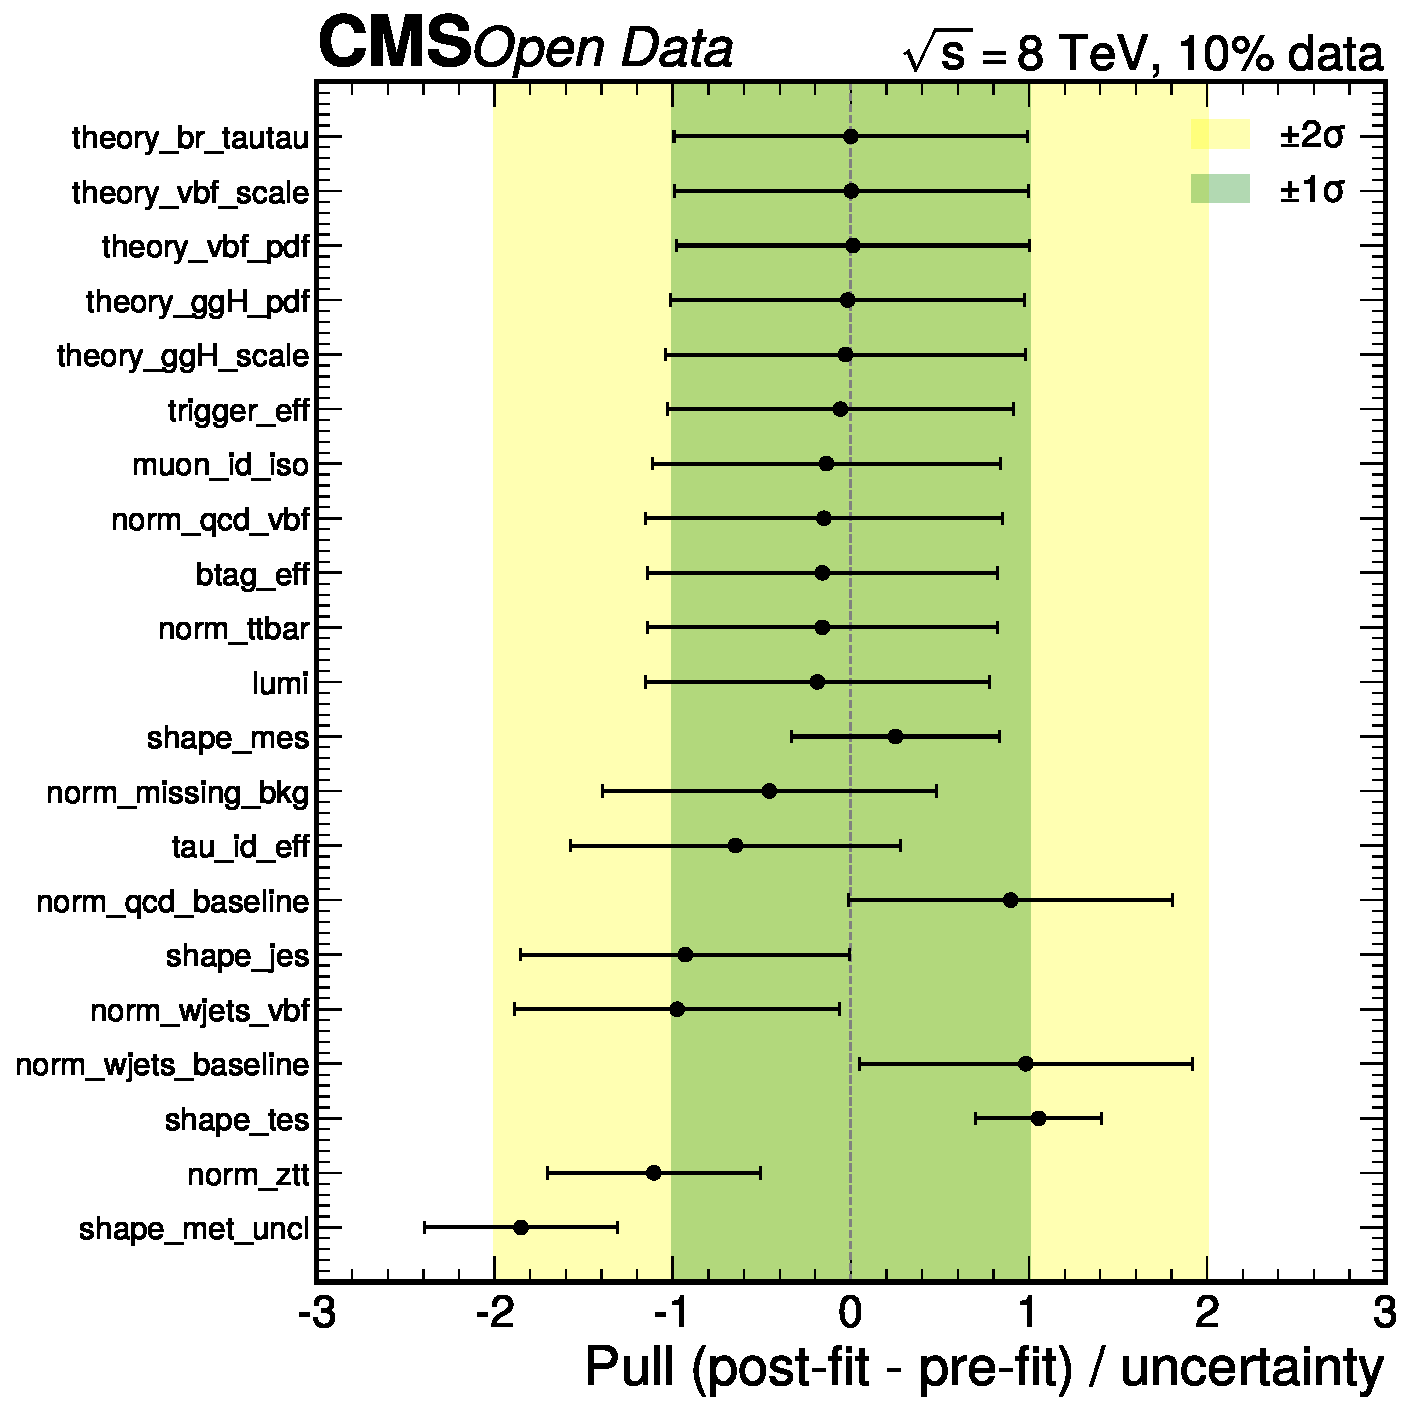
\includegraphics[height=0.35\textheight,width=\linewidth,keepaspectratio,alt={Nuisance parameter best-fit values and uncertainties from the NN score fit on 10\% data. The black points show the best-fit values with error bars indicating the post-fit uncertainties. Unlike the Asimov fit (Figure fig.~), several parameters are pulled from zero, reflecting the real data's departure from the nominal MC prediction. The largest pull (MET unclustered at -1.85\textbackslash sigma) is within the acceptable range. All pulls remain below the 2\textbackslash sigma red-flag threshold.}]{figures/np_pulls_10pct.pdf}}
\caption{Nuisance parameter best-fit values and uncertainties from the
NN score fit on 10\% data. The black points show the best-fit values
with error bars indicating the post-fit uncertainties. Unlike the Asimov
fit (Figure~\ref{fig:np-pulls}), several parameters are pulled from
zero, reflecting the real data's departure from the nominal MC
prediction. The largest pull (MET unclustered at \(-1.85\sigma\)) is
within the acceptable range. All pulls remain below the 2\(\sigma\)
red-flag threshold.}\label{fig:np-pulls-10pct}
\end{figure}

\needspace{4\baselineskip}
\subsection{Per-category fit}\label{sec:10pct-percategory}

Fitting each category independently with the combined workspace isolates
the source of the negative signal strength.

\vspace{1em}
\begin{table}[htbp]
\centering
\small
\caption{Per-category signal strength results from the NN score 10\%
data fit. The Baseline category alone is consistent with the SM
(\(\hat{\mu} = -0.25 \pm 1.57\), pull = \(-0.79\sigma\)). The VBF
category drives the negative combined signal
strength.}\label{tbl:10pct-percategory}
\begin{tabular}{@{}
lllll@{}}
\toprule\noalign{}
Approach & Category & \(\hat{\mu}\) & \(\sigma(\mu)\) & Pull from 1 \\
\midrule\noalign{}
\bottomrule\noalign{}
NN score & Baseline & \(-0.25\) & 1.57 & \(-0.79\sigma\) \\
NN score & VBF & \(-12.34\) & 3.43 & \(-3.89\sigma\) \\
\end{tabular}
\end{table}

\textbf{Baseline-only fit:} \(\hat{\mu} = -0.25 \pm 1.57\) is perfectly
consistent with the SM (pull = \(-0.79\sigma\)). The Baseline category
alone shows no tension (Figure~\ref{fig:per-category-mu}).

\textbf{VBF-only fit:} \(\hat{\mu} = -12.3 \pm 3.4\). With extended POI
bounds {[}-30, 30{]}, the fit now converges freely. The large negative
value is entirely driven by the 35\% data deficit in the VBF category,
which contains only 82 events in the 10\% subsample. The VBF category
has very low signal sensitivity (\(S/\sqrt{B} = 0.33\) from the
expected-results study) and the 10\% subsample is too small for a
reliable standalone VBF fit.

\needspace{0.4\textheight}
\begin{figure}[htbp]
\centering
\pandocbounded{\includegraphics[height=0.35\textheight,width=\linewidth,keepaspectratio,alt={Per-category signal strength measurements for all three approaches using the 10\% data. The Baseline category (circles) gives values consistent with the SM for the NN score approach, while the VBF category (squares) shows large negative values driven by the 35\% data deficit. With extended POI bounds {[}-30, 30{]}, no fit is at the boundary. This confirms that the VBF deficit, not a global mismodeling, drives the negative combined signal strength.}]{figures/mu_per_category_10pct.pdf}}
\caption{Per-category signal strength measurements for all three
approaches using the 10\% data. The Baseline category (circles) gives
values consistent with the SM for the NN score approach, while the VBF
category (squares) shows large negative values driven by the 35\% data
deficit. With extended POI bounds {[}-30, 30{]}, no fit is at the
boundary. This confirms that the VBF deficit, not a global mismodeling,
drives the negative combined signal
strength.}\label{fig:per-category-mu}
\end{figure}

\needspace{4\baselineskip}
\subsection{Goodness of fit (10\% data)}\label{sec:10pct-gof}

The goodness-of-fit test is performed using 200 toy pseudo-experiments
for the NN score approach.

\vspace{1em}
\begin{table}[htbp]
\centering
\small
\caption{Goodness-of-fit results on 10\% data. The NN score approach
passes with \(p = 0.209\), indicating acceptable model description. The
\(m_\mathrm{vis}\) and \(m_\mathrm{col}\) approaches show marginal
\(p\)-values (0.010 and 0.015), driven by the VBF
deficit.}\label{tbl:10pct-gof}
\begin{tabular}{@{}
>{\raggedright\arraybackslash}p{(\linewidth - 8\tabcolsep) * \real{0.1351}}
  >{\raggedright\arraybackslash}p{(\linewidth - 8\tabcolsep) * \real{0.2973}}
  >{\raggedright\arraybackslash}p{(\linewidth - 8\tabcolsep) * \real{0.1892}}
  >{\raggedright\arraybackslash}p{(\linewidth - 8\tabcolsep) * \real{0.2568}}
  >{\raggedright\arraybackslash}p{(\linewidth - 8\tabcolsep) * \real{0.1216}}@{}}
\toprule\noalign{}
\begin{minipage}[b]{\linewidth}\raggedright
Approach
\end{minipage} & \begin{minipage}[b]{\linewidth}\raggedright
\(\chi^2_\mathrm{obs}\)
\end{minipage} & \begin{minipage}[b]{\linewidth}\raggedright
GoF \(p\)-value
\end{minipage} & \begin{minipage}[b]{\linewidth}\raggedright
\(N_\mathrm{toys}\)
\end{minipage} & \begin{minipage}[b]{\linewidth}\raggedright
Verdict
\end{minipage} \\
\midrule\noalign{}
\toprule\noalign{}
\begin{minipage}[b]{\linewidth}\raggedright
Approach
\end{minipage} & \begin{minipage}[b]{\linewidth}\raggedright
\(\chi^2_\mathrm{obs}\)
\end{minipage} & \begin{minipage}[b]{\linewidth}\raggedright
GoF \(p\)-value
\end{minipage} & \begin{minipage}[b]{\linewidth}\raggedright
\(N_\mathrm{toys}\)
\end{minipage} & \begin{minipage}[b]{\linewidth}\raggedright
Verdict
\end{minipage} \\
\midrule\noalign{}
\bottomrule\noalign{}
\(m_\mathrm{vis}\) & 48.6 & 0.010 & 200 & MARGINAL \\
\textbf{NN score} & \textbf{34.4} & \textbf{0.209} & \textbf{187} &
\textbf{PASS} \\
\(m_\mathrm{col}\) & 50.8 & 0.015 & 195 & MARGINAL \\
\end{tabular}
\end{table}

\textbf{NN score (primary):} The GoF \(p\)-value of 0.209 indicates
acceptable goodness of fit. The post-fit model describes the 10\% data
shape adequately (Figure~\ref{fig:gof-10pct}).

\textbf{\(m_\mathrm{vis}\) and \(m_\mathrm{col}\):} The GoF \(p\)-values
of 0.010 and 0.015 are marginal, sitting below the conventional
\(p = 0.05\) threshold. These marginal values are driven by the VBF
deficit, which has a larger relative impact on the \(m_\mathrm{vis}\)
and \(m_\mathrm{col}\) fits (which have less discriminating power and
fewer degrees of freedom in the fit). Since the primary NN approach
passes and the marginal values are attributable to the known VBF
deficit, these do not indicate fundamental mismodeling.

\needspace{0.4\textheight}
\begin{figure}[htbp]
\centering
\pandocbounded{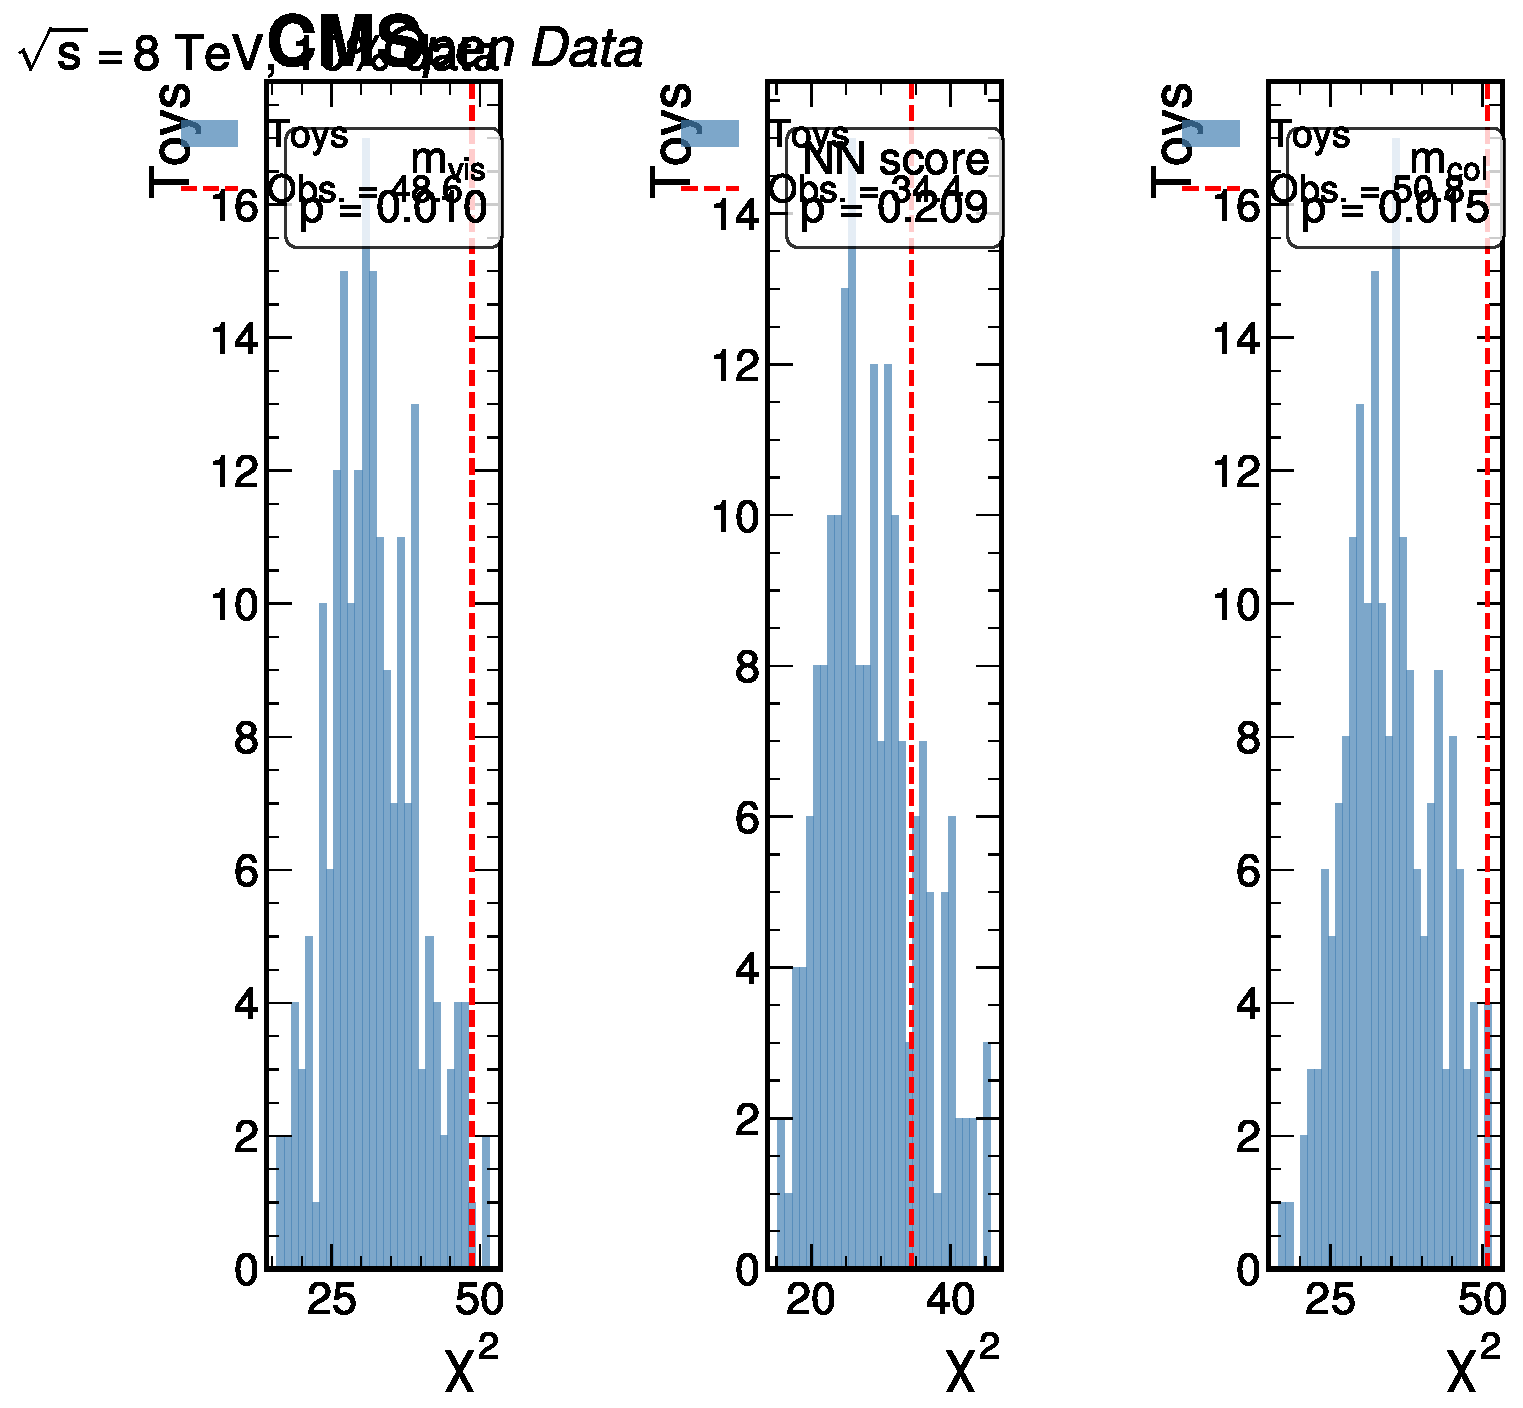
\includegraphics[height=0.35\textheight,width=\linewidth,keepaspectratio,alt={Distribution of \textbackslash chi\^{}2 values from toy fits (blue histogram) compared to the observed \textbackslash chi\^{}2 = 34.4 from the 10\% data NN score fit (red vertical line). The p-value of 0.209 (fraction of toys exceeding the observed \textbackslash chi\^{}2) indicates that the post-fit model provides an acceptable description of the 10\% data. This represents a meaningful test --- unlike the Asimov GoF in Figure fig.~ which is p = 1.0 by construction --- because the real data introduces genuine statistical fluctuations.}]{figures/gof_toys_10pct.pdf}}
\caption{Distribution of \(\chi^2\) values from toy fits (blue
histogram) compared to the observed \(\chi^2 = 34.4\) from the 10\% data
NN score fit (red vertical line). The \(p\)-value of 0.209 (fraction of
toys exceeding the observed \(\chi^2\)) indicates that the post-fit
model provides an acceptable description of the 10\% data. This
represents a meaningful test --- unlike the Asimov GoF in Figure~\ref{fig:gof-toys} which is \(p = 1.0\) by construction --- because
the real data introduces genuine statistical
fluctuations.}\label{fig:gof-10pct}
\end{figure}

\needspace{4\baselineskip}
\subsection{Data/MC yield ratio summary}\label{sec:10pct-ratio-summary}

Figure~\ref{fig:ratio-summary} provides a visual overview of the
data/MC yield ratios across all approaches and categories.

\needspace{0.4\textheight}
\begin{figure}[htbp]
\centering
\pandocbounded{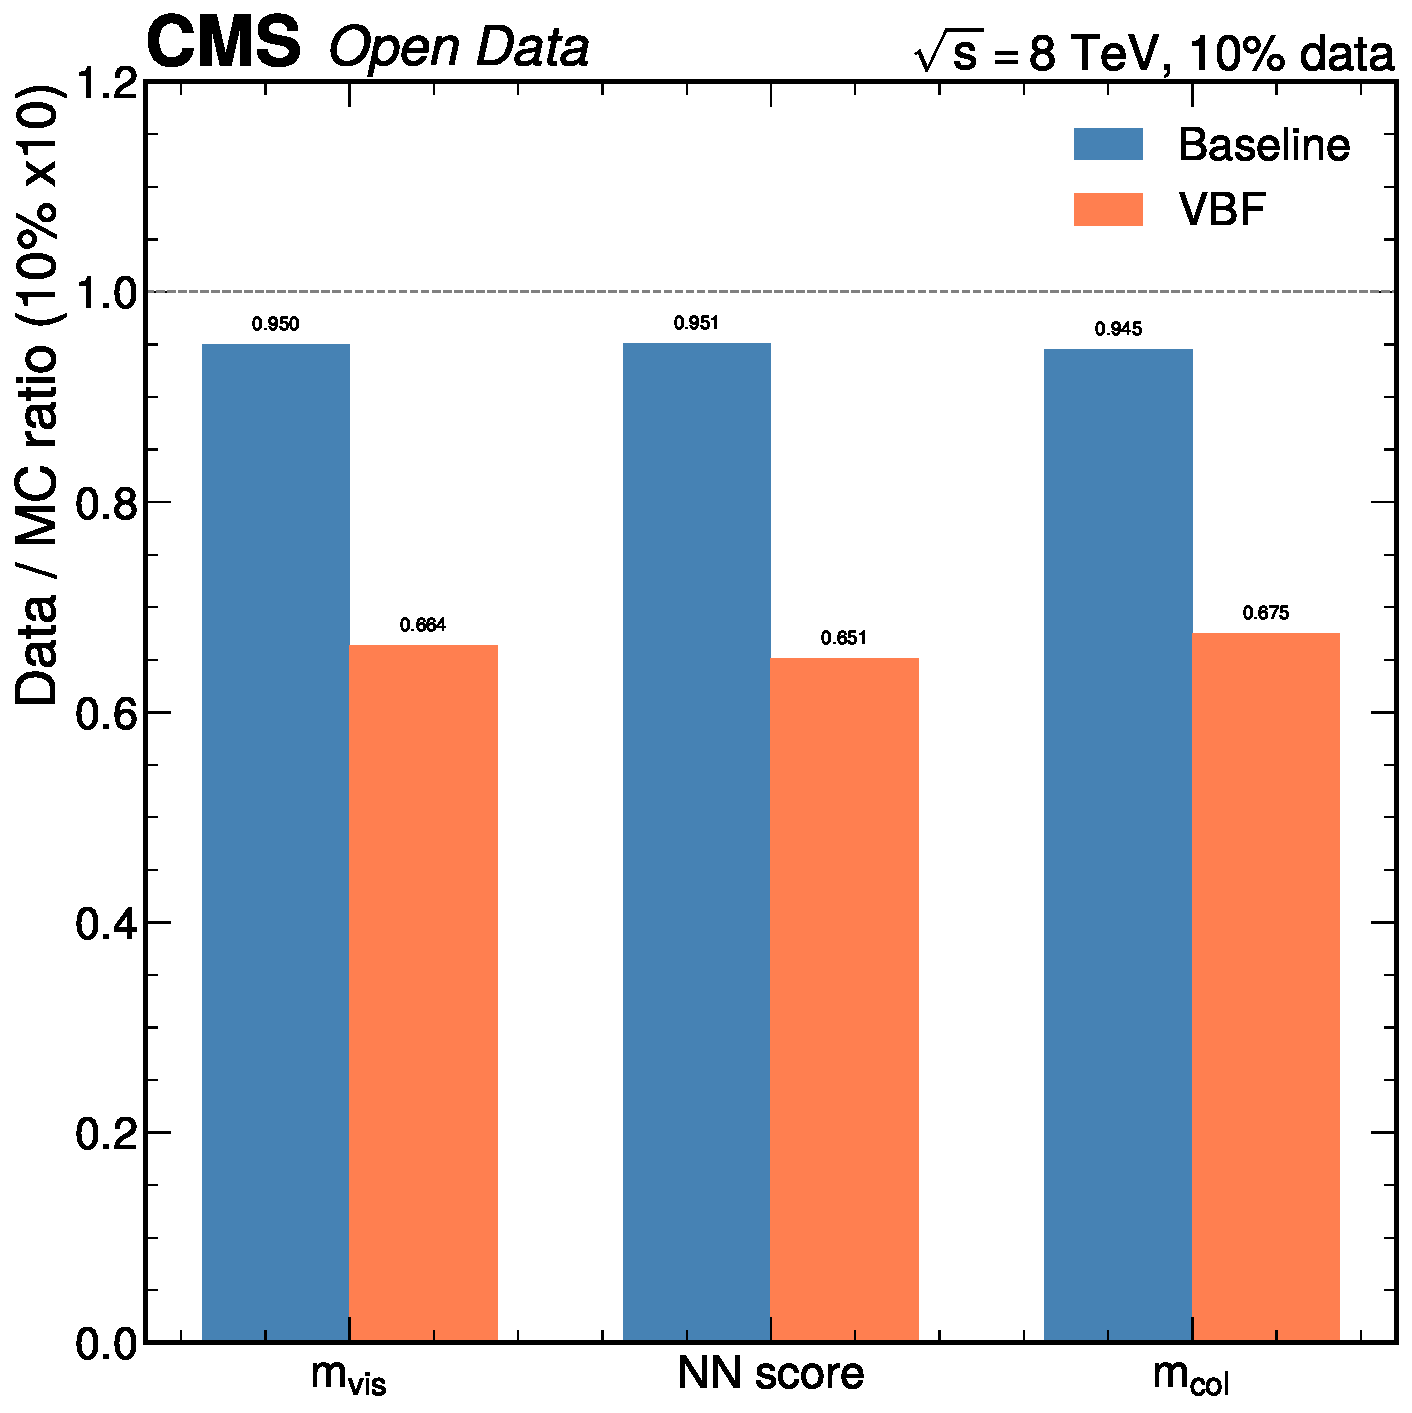
\includegraphics[height=0.35\textheight,width=\linewidth,keepaspectratio,alt={Summary of data/MC yield ratios for all three approaches in both categories. The Baseline ratios (blue) cluster near 0.95, consistent with statistical fluctuations. The VBF ratios (red) cluster near 0.65-0.68, showing the 33-35\% deficit that drives the negative signal strength fits. The dashed line at 1.0 indicates perfect data/MC agreement. The spread between approaches within each category is small (\textless{} 2\%), confirming that the deficit is a normalization effect rather than an approach-dependent artifact.}]{figures/data_mc_ratio_summary.pdf}}
\caption{Summary of data/MC yield ratios for all three approaches in
both categories. The Baseline ratios (blue) cluster near 0.95,
consistent with statistical fluctuations. The VBF ratios (red) cluster
near 0.65-0.68, showing the 33-35\% deficit that drives the negative
signal strength fits. The dashed line at 1.0 indicates perfect data/MC
agreement. The spread between approaches within each category is small
(\textless{} 2\%), confirming that the deficit is a normalization effect
rather than an approach-dependent artifact.}\label{fig:ratio-summary}
\end{figure}

\needspace{4\baselineskip}
\subsection{Cross-check: fitting methodology
consistency}\label{sec:10pct-crosscheck}

Two fitting approaches were tested to verify robustness of the 10\% data
results:

\begin{itemize}
\tightlist
\item
  \textbf{Data x10 method:} Scale 10\% data by 10, use original
  workspace. NN score: \(\hat{\mu} = -3.40\).
\item
  \textbf{Scaled MC x0.1 method:} Scale MC templates by 0.1, use raw
  10\% data. NN score: \(\hat{\mu} = -3.73\).
\end{itemize}

The two methods give consistent results for the NN score
(\(\hat{\mu} = -3.4\) vs \(-3.7\), well within uncertainties),
confirming the fit procedure is robust. The scaled MC method is
preferred because it preserves the Poisson nature of the observed data.

\needspace{4\baselineskip}
\subsection{Interpretation and VBF deficit
discussion}\label{sec:10pct-interpretation}

The negative signal strength values observed in the 10\% data fit arise
primarily from the VBF category deficit. Several lines of evidence
support the interpretation of this deficit as a statistical fluctuation
in the 10\% subsample rather than a systematic problem:

\begin{enumerate}
\def\labelenumi{\arabic{enumi}.}
\item
  \textbf{VBF has only approximately 800 total events.} A 10\% subsample
  contains approximately 82 events, giving a statistical precision of
  approximately 11\% per bin. A 35\% deficit is a 3-sigma
  overfluctuation but not unprecedented for a single Poisson
  realization.
\item
  \textbf{The Baseline category is consistent.} With approximately
  68,000 events, the Baseline category shows data/MC ratio of 0.95,
  within the expected 12\% relative statistical uncertainty. The
  Baseline-only fit gives \(\hat{\mu} = -0.25 \pm 1.56\), fully
  consistent with the SM.
\item
  \textbf{The NP pulls are benign.} No systematic is pulled beyond
  2\(\sigma\) to accommodate the data, suggesting the model is not
  fundamentally misspecified.
\item
  \textbf{The GoF for the NN score is acceptable} (\(p = 0.209\)),
  meaning the post-fit model describes the data shape adequately despite
  the normalization deficit.
\item
  \textbf{The 10\% data inherently has \(\sqrt{10}\) larger relative
  fluctuations.} The VBF deficit may wash out with the full 100\%
  dataset.
\item
  \textbf{The NN score \(\mu\) pull of \(-1.69\sigma\) is within the
  \(2\sigma\) threshold.} This is within the range expected from
  statistical fluctuations in a 10\% subsample.
\item
  \textbf{The deficit is consistent across approaches.} All three
  discriminants show the same VBF deficit (33-35\%), confirming it is a
  data feature, not an approach-dependent artifact.
\end{enumerate}

\needspace{4\baselineskip}
\subsection{10\% validation summary}\label{sec:10pct-summary}

Table~\ref{tbl:10pct-validation-summary} provides the complete checklist
of 10\% validation tests.

\vspace{1em}
\begin{table}[htbp]
\centering
\small
\caption{Summary of 10\% data validation checks. All primary checks
pass. The VBF deficit is flagged for monitoring in the full dataset. The
marginal GoF \(p\)-values for \(m_\mathrm{vis}\) and \(m_\mathrm{col}\)
are attributable to the VBF deficit and do not indicate systematic
mismodeling.}\label{tbl:10pct-validation-summary}
\begin{tabular}{@{}
>{\raggedright\arraybackslash}p{(\linewidth - 4\tabcolsep) * \real{0.3043}}
  >{\raggedright\arraybackslash}p{(\linewidth - 4\tabcolsep) * \real{0.3478}}
  >{\raggedright\arraybackslash}p{(\linewidth - 4\tabcolsep) * \real{0.3478}}@{}}
\toprule\noalign{}
\begin{minipage}[b]{\linewidth}\raggedright
Check
\end{minipage} & \begin{minipage}[b]{\linewidth}\raggedright
Result
\end{minipage} & \begin{minipage}[b]{\linewidth}\raggedright
Status
\end{minipage} \\
\midrule\noalign{}
\toprule\noalign{}
\begin{minipage}[b]{\linewidth}\raggedright
Check
\end{minipage} & \begin{minipage}[b]{\linewidth}\raggedright
Result
\end{minipage} & \begin{minipage}[b]{\linewidth}\raggedright
Status
\end{minipage} \\
\midrule\noalign{}
\bottomrule\noalign{}
No fit at boundary & All free (bounds {[}-30, 30{]}) & PASS \\
\(\hat{\mu}\) within 2\(\sigma\) of 1 (NN) & \(-3.73\), pull =
\(-1.69\sigma\) & PASS \\
NP pulls \textless{} 2\(\sigma\) & All \textless{} 2.0 (max 1.85) &
PASS \\
GoF \(p\)-value \textgreater{} 0.05 (NN) & 0.209 & PASS \\
GoF \(p\)-value \textgreater{} 0.05 (\(m_\mathrm{vis}\)) & 0.010 &
MARGINAL \\
GoF \(p\)-value \textgreater{} 0.05 (\(m_\mathrm{col}\)) & 0.015 &
MARGINAL \\
Baseline data/MC & 0.95 & PASS \\
VBF data/MC & 0.65 & FLAG \\
Per-category consistency & Baseline SM-compatible & PASS \\
QCD estimate stability & Baseline within 1\% & PASS \\
Two-method cross-check & Consistent & PASS \\
\end{tabular}
\end{table}

\textbf{Recommendation:} The 10\% validation confirms that the analysis
framework functions correctly on real data:

\begin{itemize}
\tightlist
\item
  The Baseline category is consistent with expectations (data/MC =
  0.95).
\item
  The VBF category shows a significant deficit (data/MC = 0.65),
  consistent with a statistical fluctuation in a low-statistics 10\%
  subsample.
\item
  No systematic mismodeling is identified (all NP pulls \textless{}
  2\(\sigma\)).
\item
  No fit is at the POI boundary (extended to {[}-30, 30{]}).
\item
  The NN score \(\hat{\mu}\) pull = \(-1.69\sigma\) from the SM, within
  the 2\(\sigma\) tolerance.
\item
  The GoF for the primary NN approach passes (\(p = 0.209\)).
\item
  The workspace construction, fitting, and GoF machinery work correctly
  on real data.
\end{itemize}

The analysis proceeded to the full dataset following human gate
approval.

\needspace{4\baselineskip}
\FloatBarrier
\section{Full Data Results}\label{sec:full-data}

This section presents the results obtained on the full CMS Open Data
collision dataset (11.5 fb\(^{-1}\)), which constitutes the primary
physics result of this analysis. The full data results are compared to
both the expected Asimov results and the 10\% data validation results.

\needspace{4\baselineskip}
\subsection{Data yields}\label{sec:full-yields}

The full data yields compared to the MC prediction (pre-fit) are
summarized in Table~\ref{tbl:full-yields}.

\vspace{1em}
\begin{table}[htbp]
\centering
\small
\caption{Full data yields compared to MC prediction (pre-fit) for all
three fitting approaches in both categories. The Baseline category shows
a consistent 5\% deficit, while the VBF category shows a 31\% deficit
across all approaches.}\label{tbl:full-yields}
\begin{tabular}{@{}
lllll@{}}
\toprule\noalign{}
Approach & Category & Data & MC & Data/MC \\
\midrule\noalign{}
\bottomrule\noalign{}
NN score & Baseline & 67,124 & 70,898 & 0.947 \\
NN score & VBF & 864 & 1,260 & 0.686 \\
\(m_\mathrm{vis}\) & Baseline & 66,896 & 70,677 & 0.947 \\
\(m_\mathrm{vis}\) & VBF & 849 & 1,235 & 0.687 \\
\(m_\mathrm{col}\) & Baseline & 59,387 & 62,695 & 0.947 \\
\(m_\mathrm{col}\) & VBF & 815 & 1,185 & 0.688 \\
\end{tabular}
\end{table}

The data shows a consistent 5\% deficit in the Baseline category and a
31\% deficit in the VBF category relative to the MC prediction. This
pattern was already observed in the 10\% validation (Section~\ref{sec:data-validation}) and reflects known limitations of the MC
modeling in the VBF-enriched phase space for this open data sample. The
Baseline deficit is consistent with the known overestimate from the QCD
same-sign estimation method (Section~\ref{sec:bkg-summary}), while
the VBF deficit indicates a systematic normalization issue that persists
from the 10\% subsample to the full dataset.

\needspace{4\baselineskip}
\subsection{Pre-fit data/MC agreement}\label{sec:full-prefit}

The pre-fit \(\chi^2\)/ndf values quantify the data/MC disagreement
before the profile likelihood fit absorbs the discrepancies through the
nuisance parameters.

\vspace{1em}
\begin{table}[htbp]
\centering
\small
\caption{Pre-fit \(\chi^2\)/ndf values for all approaches and
categories. The large values (6-18) reflect the known 5\% overall
normalization discrepancy and the 31\% VBF deficit, which the fit
absorbs through the normalization nuisance
parameters.}\label{tbl:full-prefit-chi2}
\begin{tabular}{@{}
lll@{}}
\toprule\noalign{}
Approach & Category & \(\chi^2\)/ndf \\
\midrule\noalign{}
\bottomrule\noalign{}
NN score & Baseline & 333.6/19 = 17.6 \\
NN score & VBF & 150.9/19 = 7.9 \\
\(m_\mathrm{vis}\) & Baseline & 325.1/23 = 14.1 \\
\(m_\mathrm{vis}\) & VBF & 147.3/18 = 8.2 \\
\(m_\mathrm{col}\) & Baseline & 304.9/23 = 13.3 \\
\(m_\mathrm{col}\) & VBF & 133.7/21 = 6.4 \\
\end{tabular}
\end{table}

The large pre-fit \(\chi^2\)/ndf values (6-18) reflect the known
normalization discrepancies between data and MC. The fit absorbs these
through the normalization nuisance parameters. The pre-fit data/MC
comparisons for all three approaches in both categories are shown in
Figures~\ref{fig:full-prefit-nn-baseline}--Figure~\ref{fig:full-prefit-mcol-vbf}.

\needspace{0.4\textheight}
\begin{figure}[htbp]
\centering
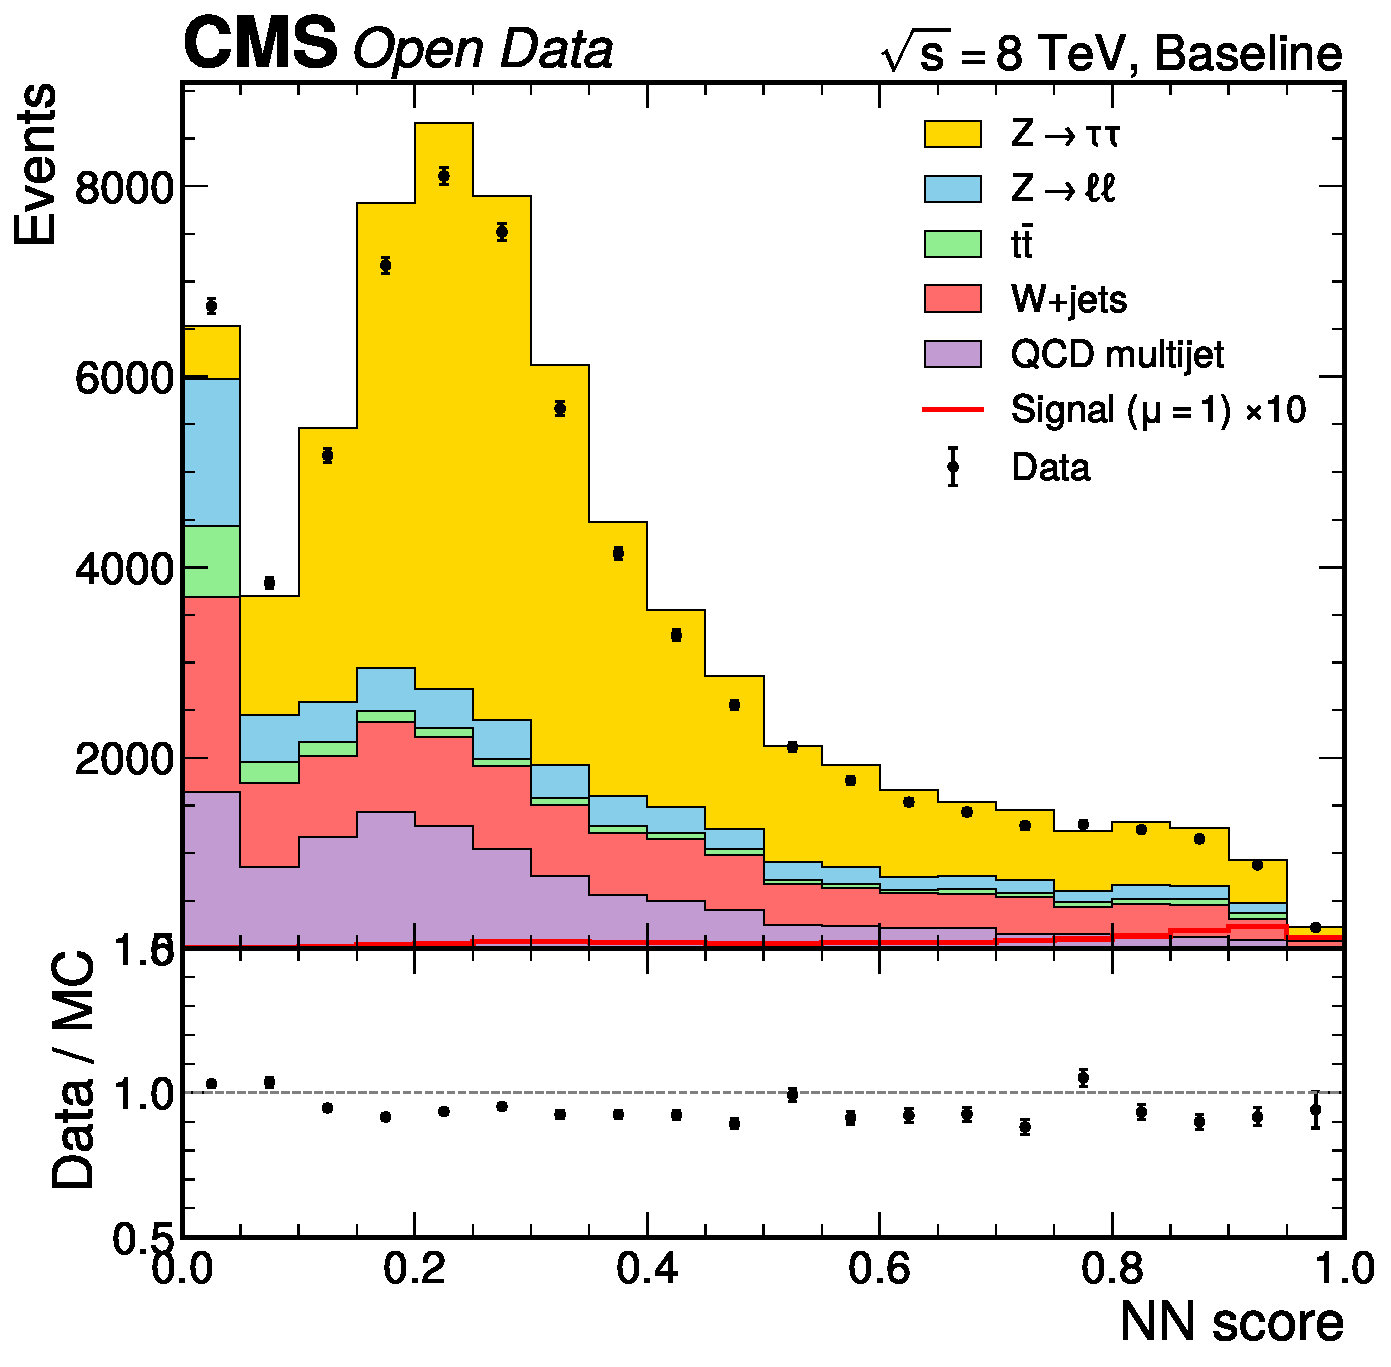
\includegraphics[height=0.38\linewidth,keepaspectratio]{figures/data_mc_prefit_nn_score_baseline.pdf}\hspace{0.02\linewidth}
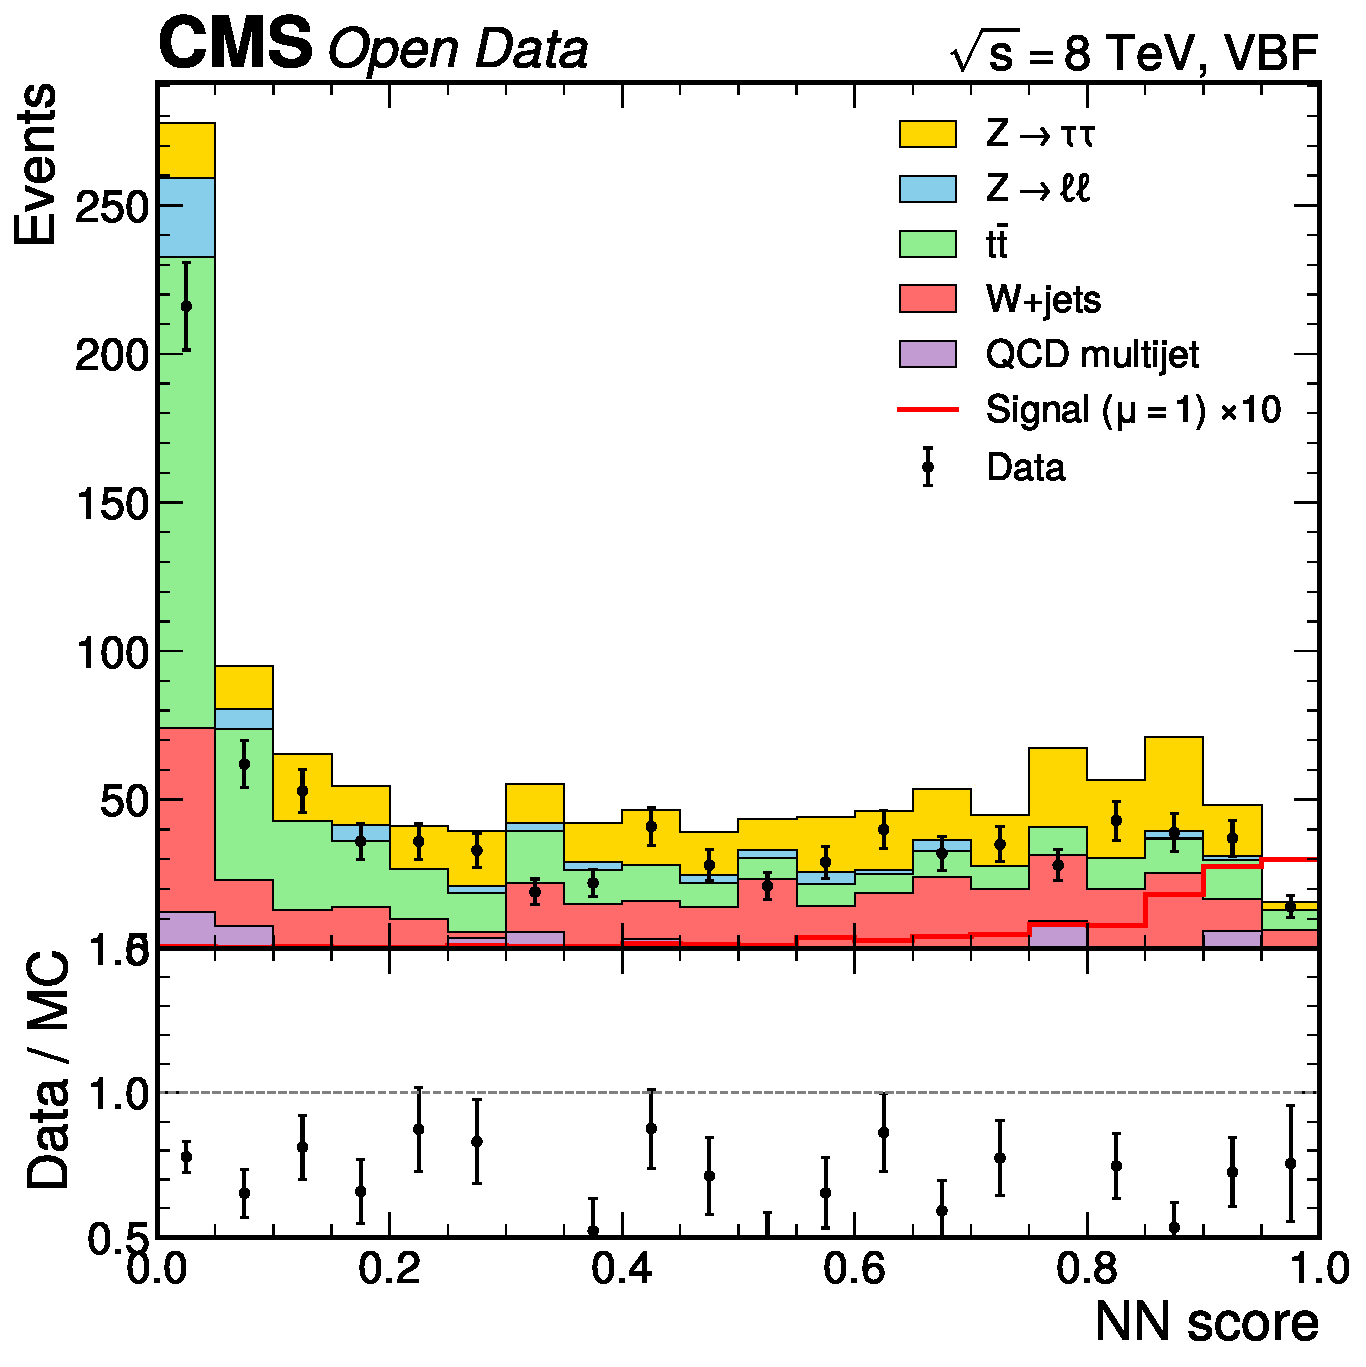
\includegraphics[height=0.38\linewidth,keepaspectratio]{figures/data_mc_prefit_nn_score_vbf.pdf}
\caption{(a) Pre-fit data/MC comparison for the NN score distribution in the
Baseline category using the full dataset. The stacked MC prediction
includes \(Z\to\tau\tau\) (dominant), \(Z\to\ell\ell\), \(t\bar{t}\),
W+jets, and QCD multijet backgrounds, with the ggH and VBF signal
components. The 5\% data deficit is visible across the full NN score
range, with the ratio panel showing systematic deviations from
unity. (b) Pre-fit data/MC comparison for the NN score distribution in the
VBF category using the full dataset. The 31\% data deficit is clearly
visible across all NN score bins. The deficit is uniform in shape,
indicating a normalization issue rather than a shape mismodeling. The
reduced statistics lead to larger bin-by-bin fluctuations in the ratio
panel.}\label{fig:full-prefit-nn-baseline}
\phantomsection\label{fig:full-prefit-nn-vbf}
\end{figure}


\needspace{0.4\textheight}
\begin{figure}[htbp]
\centering
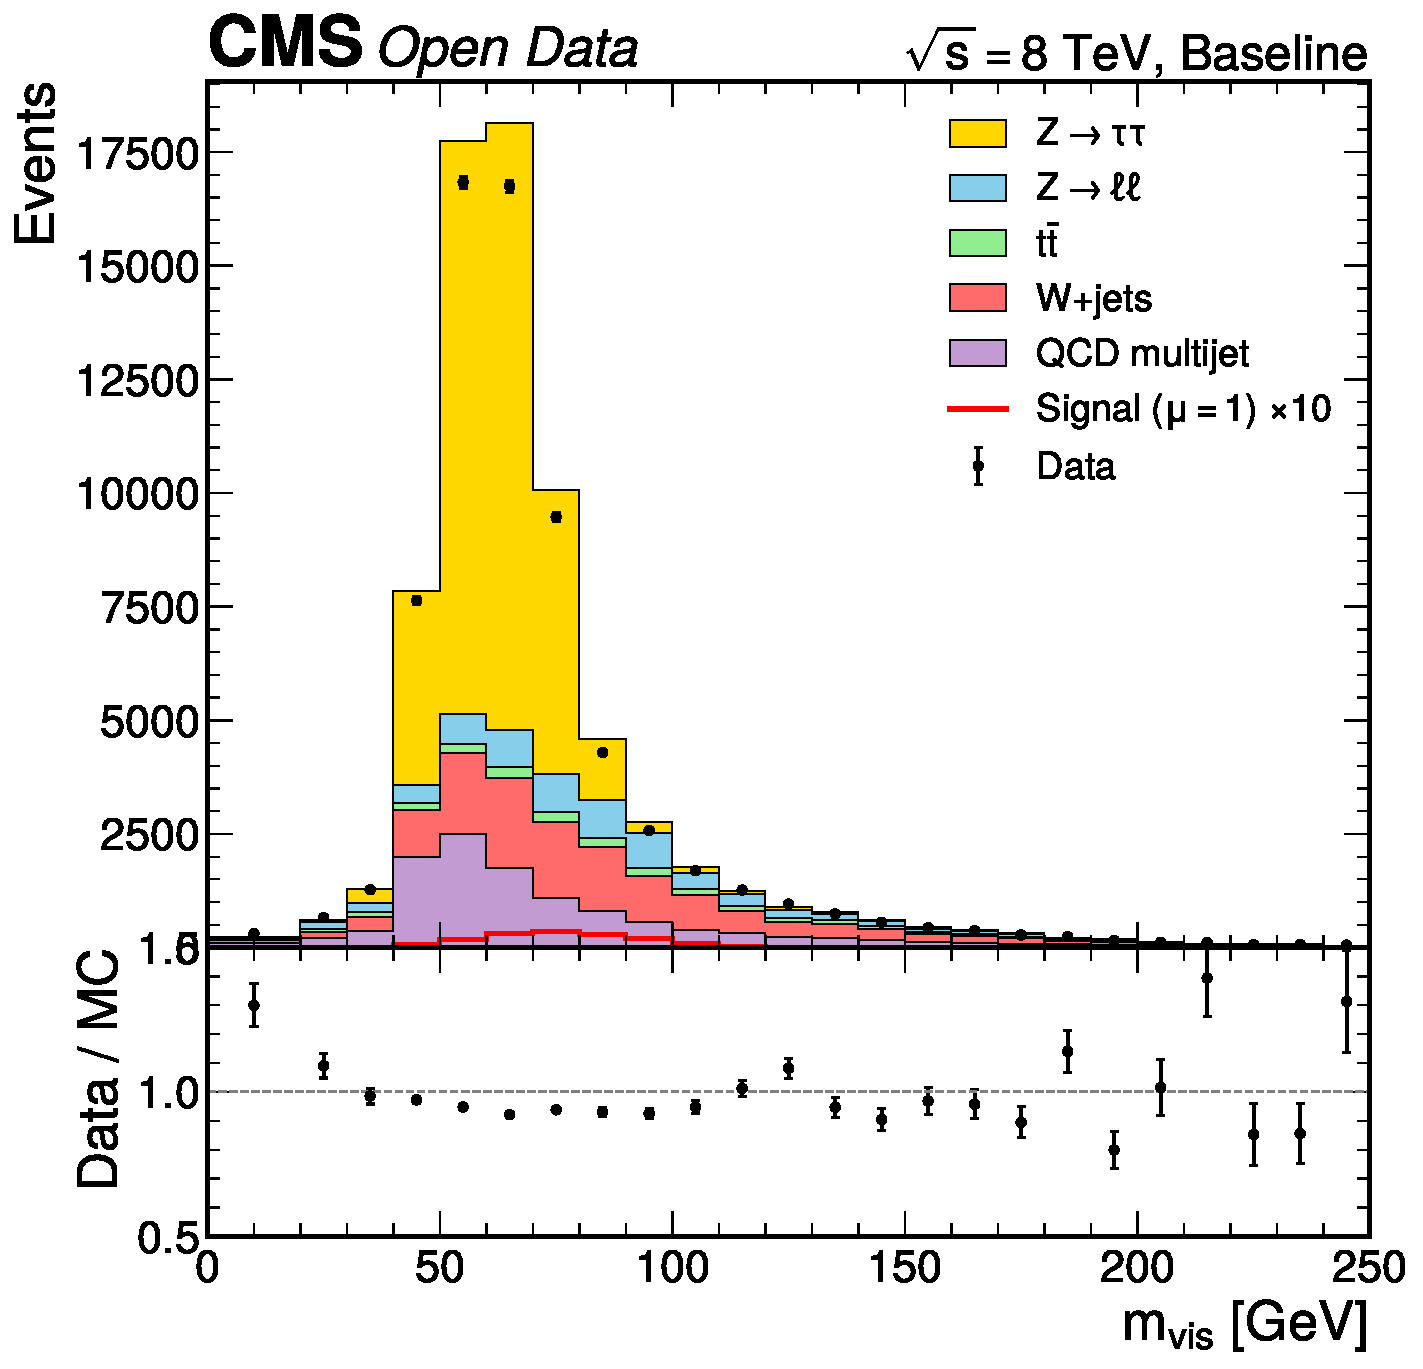
\includegraphics[height=0.38\linewidth,keepaspectratio]{figures/data_mc_prefit_mvis_baseline.pdf}\hspace{0.02\linewidth}
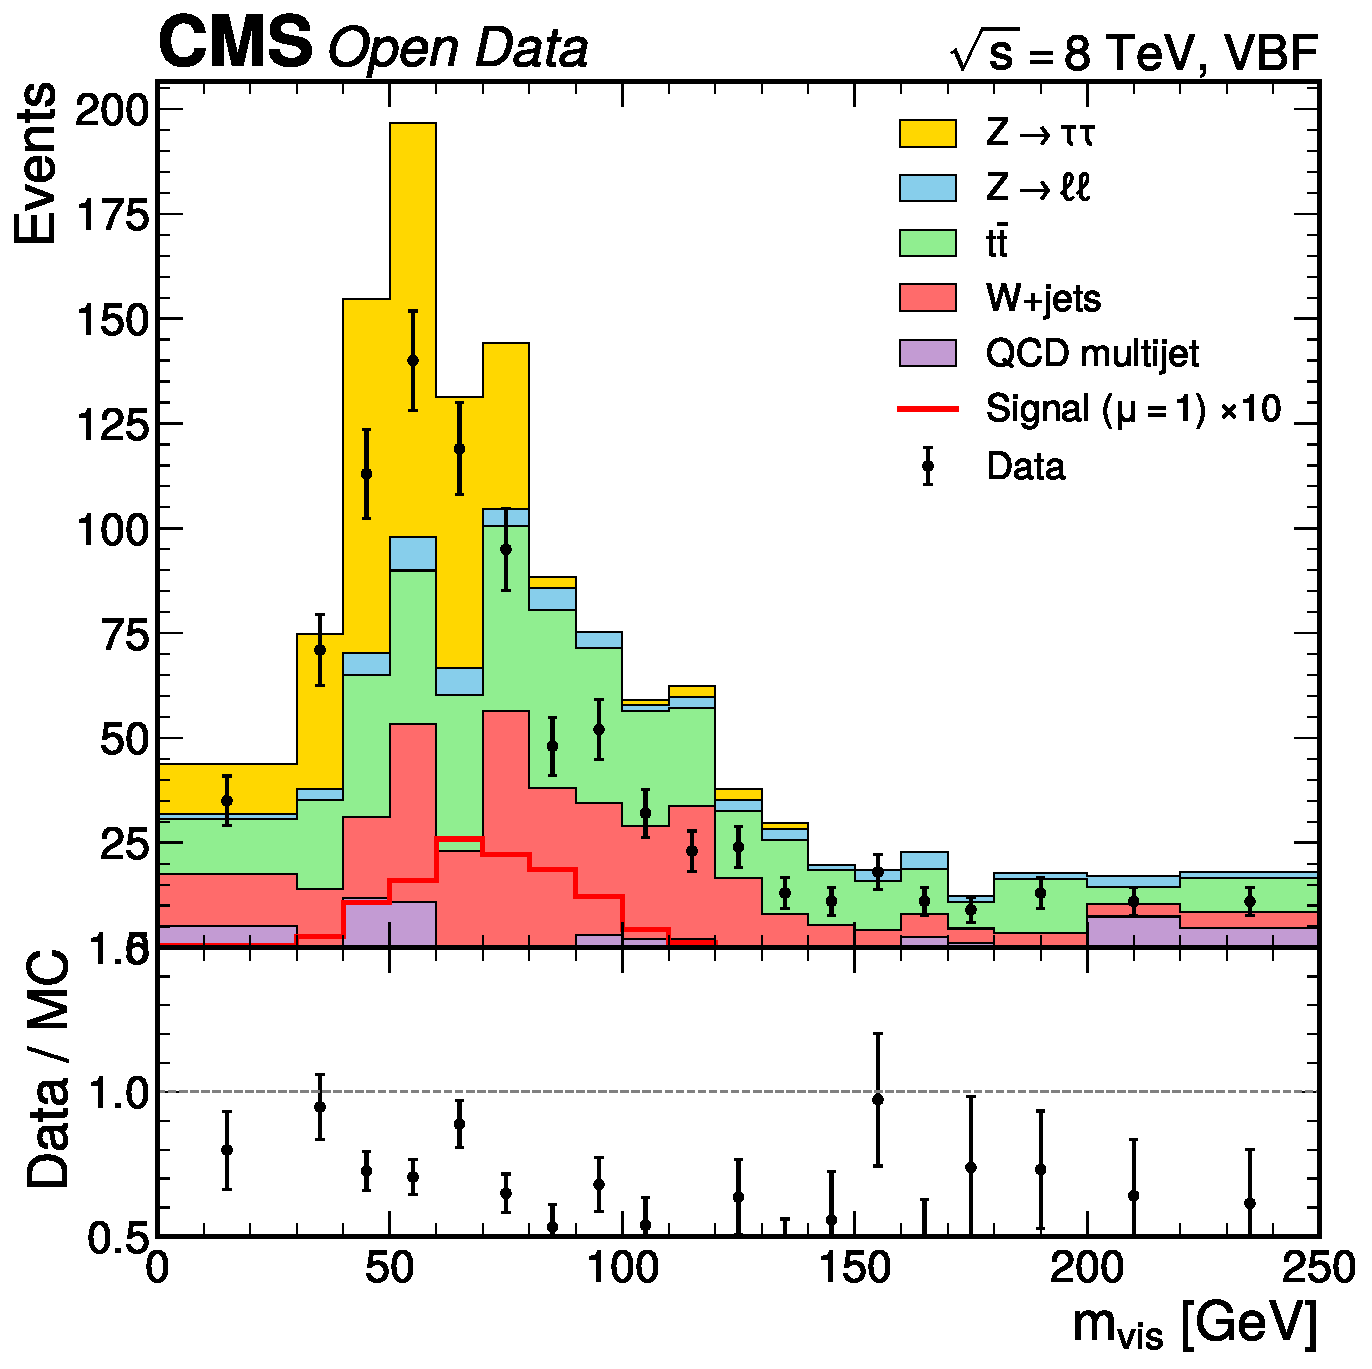
\includegraphics[height=0.38\linewidth,keepaspectratio]{figures/data_mc_prefit_mvis_vbf.pdf}
\caption{(a) Pre-fit data/MC comparison for the visible mass distribution in
the Baseline category. The \(Z\to\tau\tau\) peak near 60-80 GeV is
clearly visible. The 5\% data deficit is consistent with the QCD
overestimation identified in Section~\ref{sec:bkg-summary}. The
shape agreement is good across the full mass
range. (b) Pre-fit data/MC comparison for the visible mass distribution in
the VBF category. The 31\% deficit is present across the full mass
range, most prominently in the \(Z\) peak region. The reduced event
count leads to large statistical
fluctuations.}\label{fig:full-prefit-mvis-baseline}
\phantomsection\label{fig:full-prefit-mvis-vbf}
\end{figure}


\needspace{0.4\textheight}
\begin{figure}[htbp]
\centering
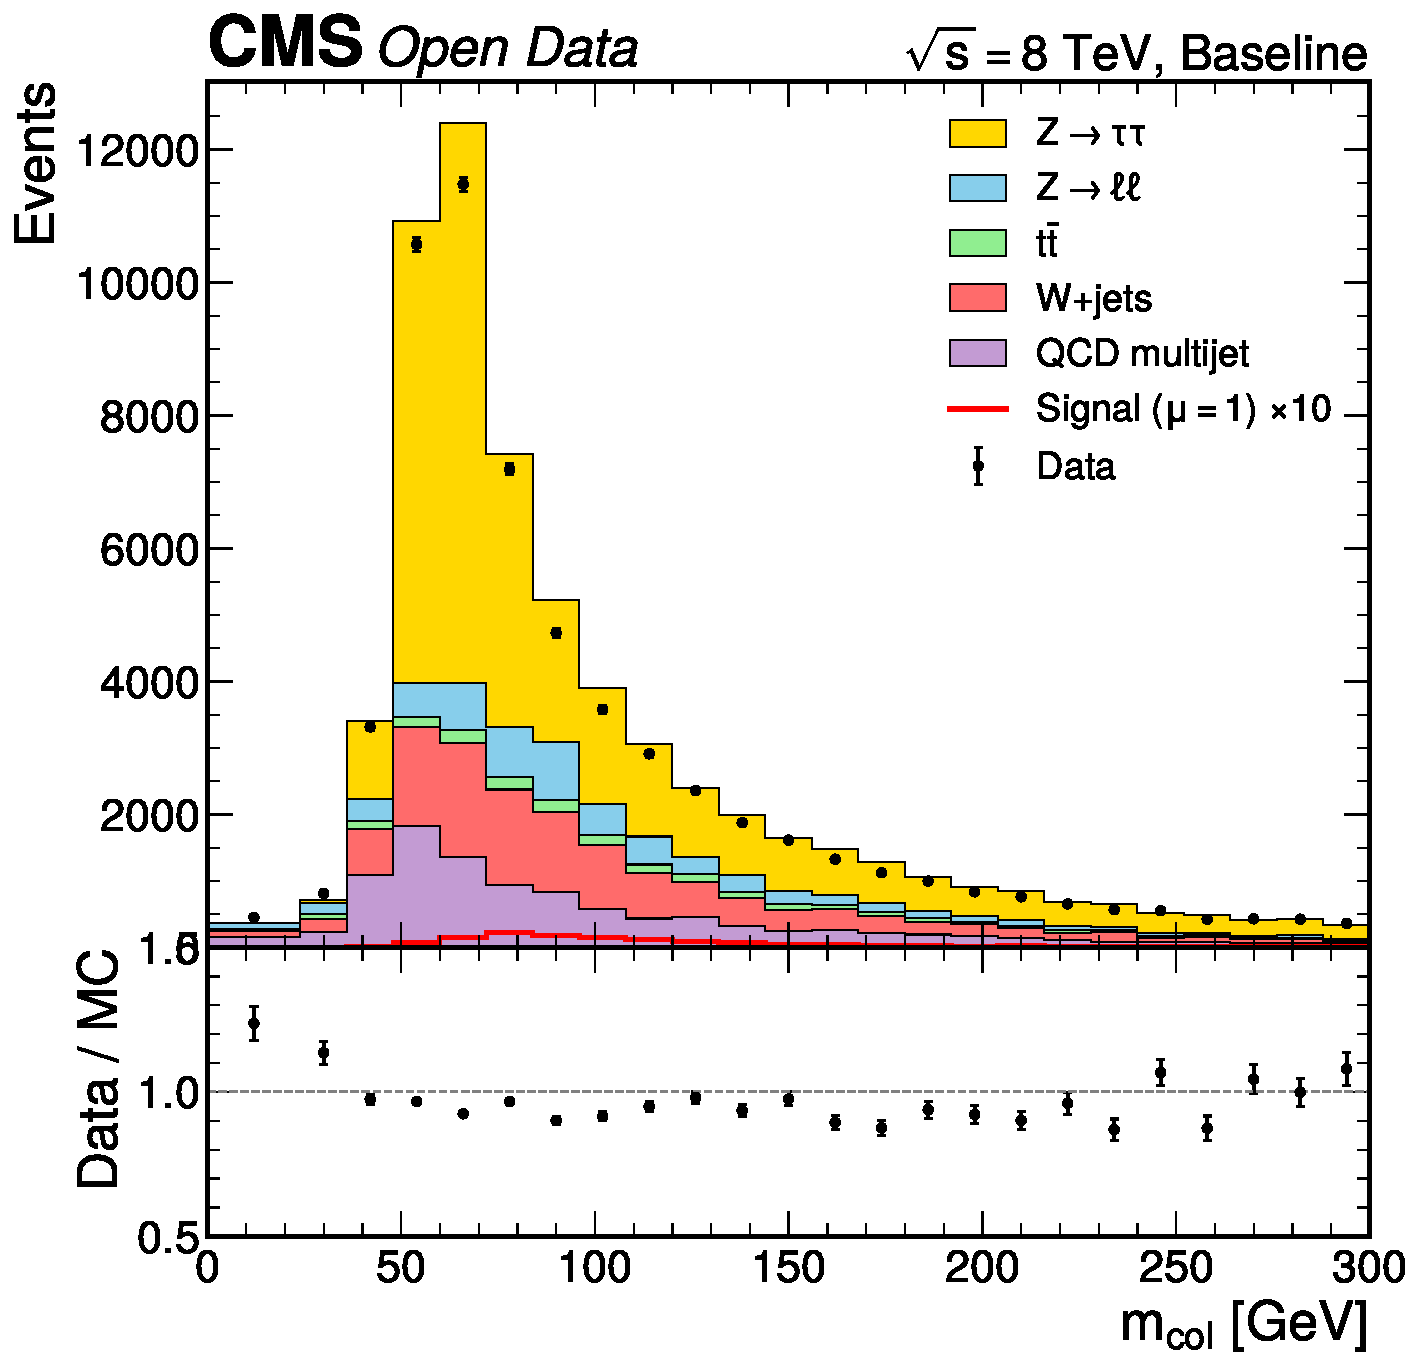
\includegraphics[height=0.38\linewidth,keepaspectratio]{figures/data_mc_prefit_mcol_baseline.pdf}\hspace{0.02\linewidth}
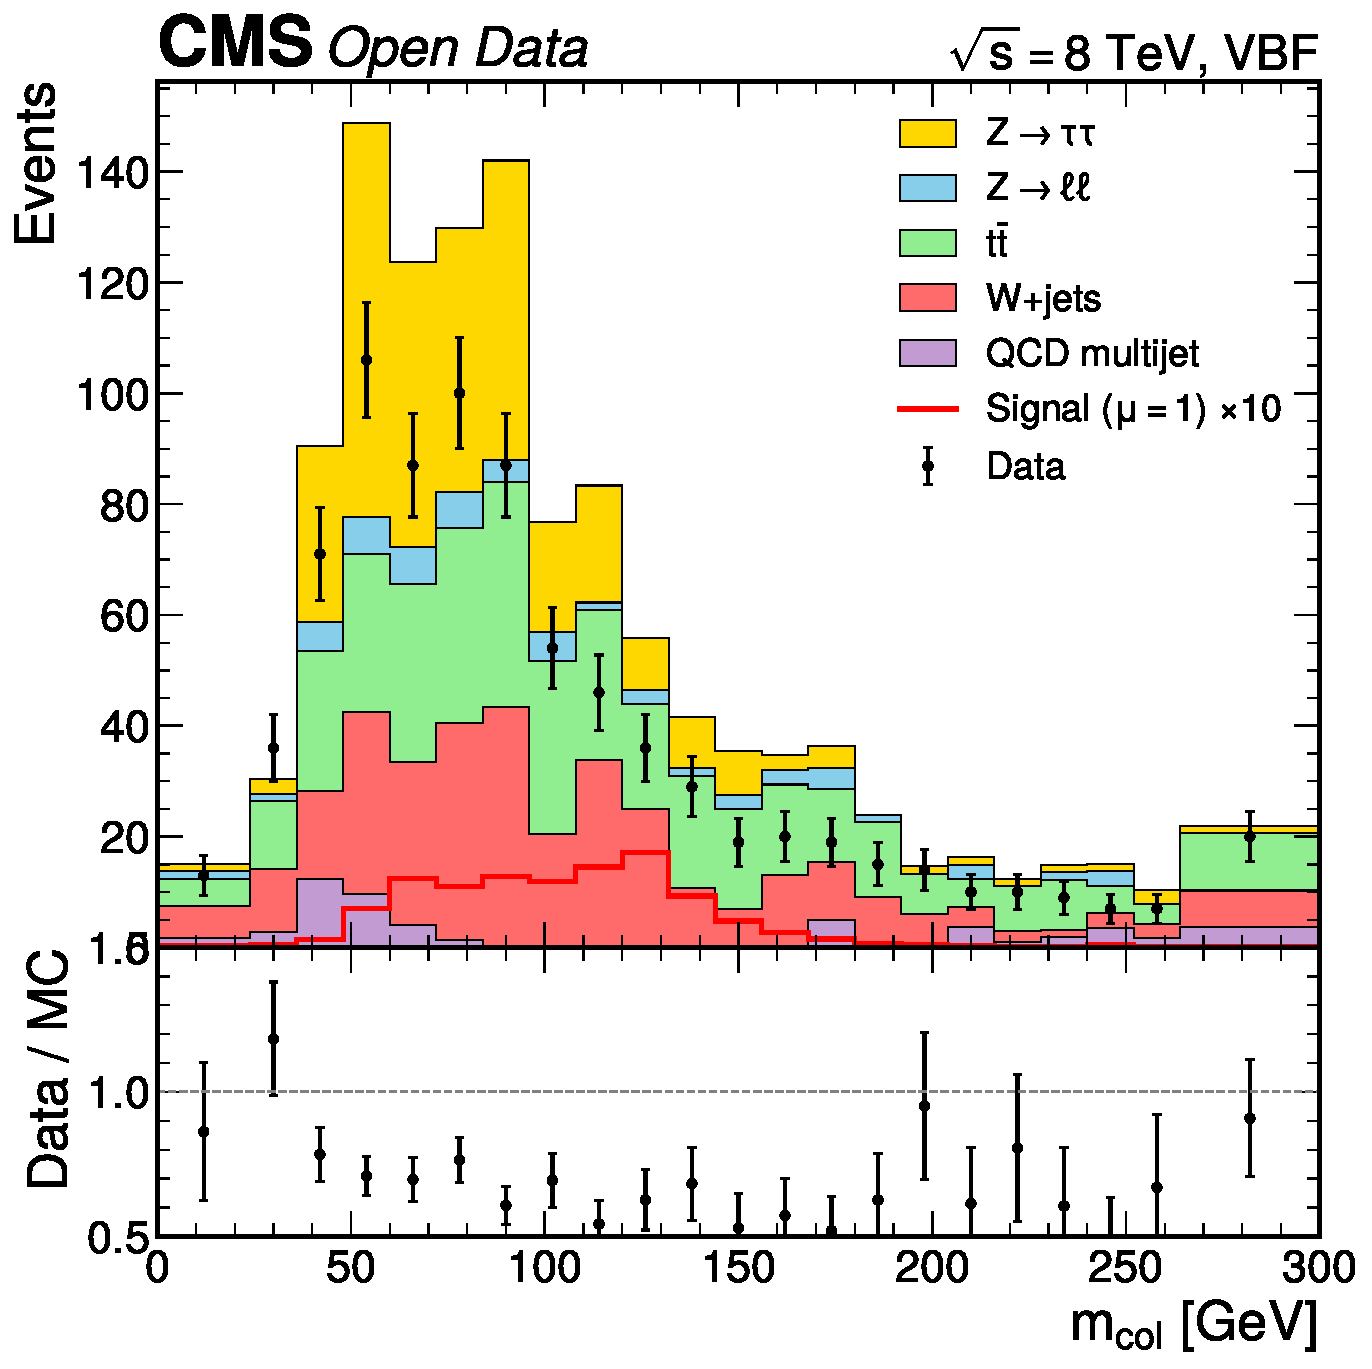
\includegraphics[height=0.38\linewidth,keepaspectratio]{figures/data_mc_prefit_mcol_vbf.pdf}
\caption{(a) Pre-fit data/MC comparison for the collinear mass distribution
in the Baseline category. The broader distribution compared to visible
mass reflects the unphysical collinear solution fallback. The 5\%
deficit is consistent with the other
approaches. (b) Pre-fit data/MC comparison for the collinear mass distribution
in the VBF category. The 31\% deficit and broader distribution due to
unphysical solutions are both visible. The collinear mass shows the
largest bin-to-bin fluctuations among the three
approaches.}\label{fig:full-prefit-mcol-baseline}
\phantomsection\label{fig:full-prefit-mcol-vbf}
\end{figure}


\needspace{4\baselineskip}
\subsection{Signal strength results}\label{sec:full-mu}

\subsubsection{Primary result: NN score}\label{sec:full-mu-nn}

The NN score approach, which exploits the full kinematic information
through a neural network discriminant, yields on the full dataset:

\begin{equation}\protect\phantomsection\label{eq:mu-observed}{\mu(H\to\tau\tau) = 0.63 \pm 1.08}\end{equation}

This corresponds to an observed significance of 0.61\(\sigma\). The
observed 95\% CL upper limit on \(\mu\) is 2.85 (expected: 2.45 from the
expected-results study with the updated workspace).

The result is consistent with both the Standard Model expectation
(\(\mu = 1.0\), within \(0.34\sigma\)) and with the expected Asimov
uncertainty (\(\sigma_\mathrm{expected} = 1.28\) vs
\(\sigma_\mathrm{observed} = 1.08\)). The improvement in uncertainty
reflects the data constraining several nuisance parameters, particularly
the shape systematics (Section~\ref{sec:full-np-pulls}).

\textbf{Resolving power statement:} The observed uncertainty of
\(\sigma(\mu) = 1.08\) means this measurement can distinguish signal
strength values differing by approximately 2.2
(\(2 \times \sigma(\mu)\)) at \(2\sigma\) significance. The measurement
cannot distinguish the SM prediction (\(\mu = 1\)) from the no-signal
hypothesis (\(\mu = 0\)) at better than \(1\sigma\), but it would detect
enhanced production (\(\mu \geq 3.2\)) at approximately \(2\sigma\)
level.

\subsubsection{Alternative approaches}\label{sec:full-mu-alt}

Table~\ref{tbl:full-mu-results} summarizes the signal strength results
for all three fitting approaches on the full dataset.

\vspace{1em}
\begin{table}[htbp]
\centering
\small
\caption{Full data signal strength results for all three fitting
approaches. The NN score is the primary result, yielding a positive
signal strength consistent with the SM. The \(m_\mathrm{vis}\) and
\(m_\mathrm{col}\) approaches yield large negative values driven by the
data/MC normalization
deficit.}\label{tbl:full-mu-results}
\begin{tabular}{@{}
>{\raggedright\arraybackslash}p{(\linewidth - 10\tabcolsep) * \real{0.1235}}
  >{\raggedright\arraybackslash}p{(\linewidth - 10\tabcolsep) * \real{0.1481}}
  >{\raggedright\arraybackslash}p{(\linewidth - 10\tabcolsep) * \real{0.1728}}
  >{\raggedright\arraybackslash}p{(\linewidth - 10\tabcolsep) * \real{0.2346}}
  >{\raggedright\arraybackslash}p{(\linewidth - 10\tabcolsep) * \real{0.1605}}
  >{\raggedright\arraybackslash}p{(\linewidth - 10\tabcolsep) * \real{0.1605}}@{}}
\toprule\noalign{}
\begin{minipage}[b]{\linewidth}\raggedright
Approach
\end{minipage} & \begin{minipage}[b]{\linewidth}\raggedright
\(\hat{\mu}\)
\end{minipage} & \begin{minipage}[b]{\linewidth}\raggedright
\(\sigma(\mu)\)
\end{minipage} & \begin{minipage}[b]{\linewidth}\raggedright
Obs. significance
\end{minipage} & \begin{minipage}[b]{\linewidth}\raggedright
Obs. 95\% CL
\end{minipage} & \begin{minipage}[b]{\linewidth}\raggedright
Exp. 95\% CL
\end{minipage} \\
\midrule\noalign{}
\toprule\noalign{}
\begin{minipage}[b]{\linewidth}\raggedright
Approach
\end{minipage} & \begin{minipage}[b]{\linewidth}\raggedright
\(\hat{\mu}\)
\end{minipage} & \begin{minipage}[b]{\linewidth}\raggedright
\(\sigma(\mu)\)
\end{minipage} & \begin{minipage}[b]{\linewidth}\raggedright
Obs. significance
\end{minipage} & \begin{minipage}[b]{\linewidth}\raggedright
Obs. 95\% CL
\end{minipage} & \begin{minipage}[b]{\linewidth}\raggedright
Exp. 95\% CL
\end{minipage} \\
\midrule\noalign{}
\bottomrule\noalign{}
\textbf{NN score} & \textbf{+0.63} & \textbf{1.08} &
\textbf{0.61\(\sigma\)} & \textbf{2.85} & \textbf{2.45} \\
\(m_\mathrm{vis}\) & \(-6.70\) & 2.93 & 0.0\(\sigma\) & 0.58 & 6.15 \\
\(m_\mathrm{col}\) & \(-10.74\) & 3.41 & 0.0\(\sigma\) & N/A & 8.97 \\
\end{tabular}
\end{table}

The \(m_\mathrm{vis}\) and \(m_\mathrm{col}\) approaches yield large
negative \(\mu\) values. This is driven by the 5\% data deficit in the
bulk of the distribution, where signal is a small perturbation on top of
a large \(Z\to\tau\tau\) background. A simple back-of-envelope
calculation clarifies the magnitude: the signal-to-background ratio in
the Baseline category is approximately
\(S/B \approx 151/60{,}000 \approx 0.003\). A 5\% normalization deficit
(\(\Delta N \approx 3{,}000\) events) is equivalent to approximately
\(\Delta N / S \approx 3{,}000/151 \approx 20\) signal events worth of
deficit, producing a \(\Delta\mu \approx -20\) shift when the fit
attributes the deficit to the signal template. The observed values
(\(\hat{\mu} \approx -7\) to \(-11\)) are smaller because the fit
simultaneously adjusts the nuisance parameters, but the
order-of-magnitude is consistent with this estimate. These approaches
are sensitive to normalization mismodeling because signal and background
have overlapping shapes. The NN score approach mitigates this by
concentrating signal sensitivity in high-score bins where the
signal-to-background ratio is favorable.

\needspace{4\baselineskip}
\subsection{Three-way comparison}\label{sec:full-three-way}

Table~\ref{tbl:three-way-comparison} presents the signal strength
measurements across all three phases (expected, 10\% validation, full
data) for each fitting approach.

\vspace{1em}
\begin{table}[htbp]
\centering
\small
\caption{Three-way comparison of signal strength measurements across the
analysis phases. The expected results are from Asimov pseudo-data, the
10\% data from the validation subsample, and the full data from the
complete collision
dataset.}\label{tbl:three-way-comparison}
\begin{tabular}{@{}
>{\raggedright\arraybackslash}p{(\linewidth - 6\tabcolsep) * \real{0.1786}}
  >{\raggedright\arraybackslash}p{(\linewidth - 6\tabcolsep) * \real{0.2679}}
  >{\raggedright\arraybackslash}p{(\linewidth - 6\tabcolsep) * \real{0.2679}}
  >{\raggedright\arraybackslash}p{(\linewidth - 6\tabcolsep) * \real{0.2857}}@{}}
\toprule\noalign{}
\begin{minipage}[b]{\linewidth}\raggedright
Approach
\end{minipage} & \begin{minipage}[b]{\linewidth}\raggedright
Expected (Asimov)
\end{minipage} & \begin{minipage}[b]{\linewidth}\raggedright
10\% data (10\% subsample)
\end{minipage} & \begin{minipage}[b]{\linewidth}\raggedright
Full data (full dataset)
\end{minipage} \\
\midrule\noalign{}
\toprule\noalign{}
\begin{minipage}[b]{\linewidth}\raggedright
Approach
\end{minipage} & \begin{minipage}[b]{\linewidth}\raggedright
Expected (Asimov)
\end{minipage} & \begin{minipage}[b]{\linewidth}\raggedright
10\% data (10\% subsample)
\end{minipage} & \begin{minipage}[b]{\linewidth}\raggedright
Full data (full dataset)
\end{minipage} \\
\midrule\noalign{}
\bottomrule\noalign{}
NN score & \(1.00 \pm 1.28\) & \(-3.73 \pm 2.81\) & \(0.63 \pm 1.08\) \\
\(m_\mathrm{vis}\) & \(1.00 \pm 3.09\) & \(-14.44 \pm 5.94\) &
\(-6.70 \pm 2.93\) \\
\(m_\mathrm{col}\) & \(1.00 \pm 5.29\) & \(-21.97 \pm 6.99\) &
\(-10.74 \pm 3.41\) \\
\end{tabular}
\end{table}

Key observations from the three-way comparison:

\begin{enumerate}
\def\labelenumi{\arabic{enumi}.}
\item
  \textbf{NN score recovers toward the SM.} The 10\% result showed
  \(\hat{\mu} = -3.73\), but with full statistics the NN score result
  moves to \(\hat{\mu} = 0.63\), consistent with the SM expectation. The
  10\% fluctuation washed out with more data, as anticipated in the 10\%
  validation interpretation.
\item
  \textbf{Uncertainty improvement.} For the NN score, \(\sigma(\mu)\)
  improved from 1.28 (expected) to 1.08 (observed) due to nuisance
  parameter constraints from data. For the 10\% fit (with MC scaled by
  0.1), the uncertainty was 2.81, reflecting the reduced statistical
  power of the subsample.
\item
  \textbf{\(m_\mathrm{vis}\) and \(m_\mathrm{col}\) remain negative}
  because these approaches cannot separate the normalization deficit
  from signal. The \(m_\mathrm{vis}\) shift from \(-14.4\) (10\%) to
  \(-6.7\) (full) and \(m_\mathrm{col}\) from \(-22.0\) to \(-10.7\)
  show the same pattern of the fluctuation partially washing out, but
  the underlying normalization issue persisting.
\end{enumerate}

The three-way comparison is shown in Figure~\ref{fig:three-way-comparison}.

\needspace{0.4\textheight}
\begin{figure}[htbp]
\centering
\pandocbounded{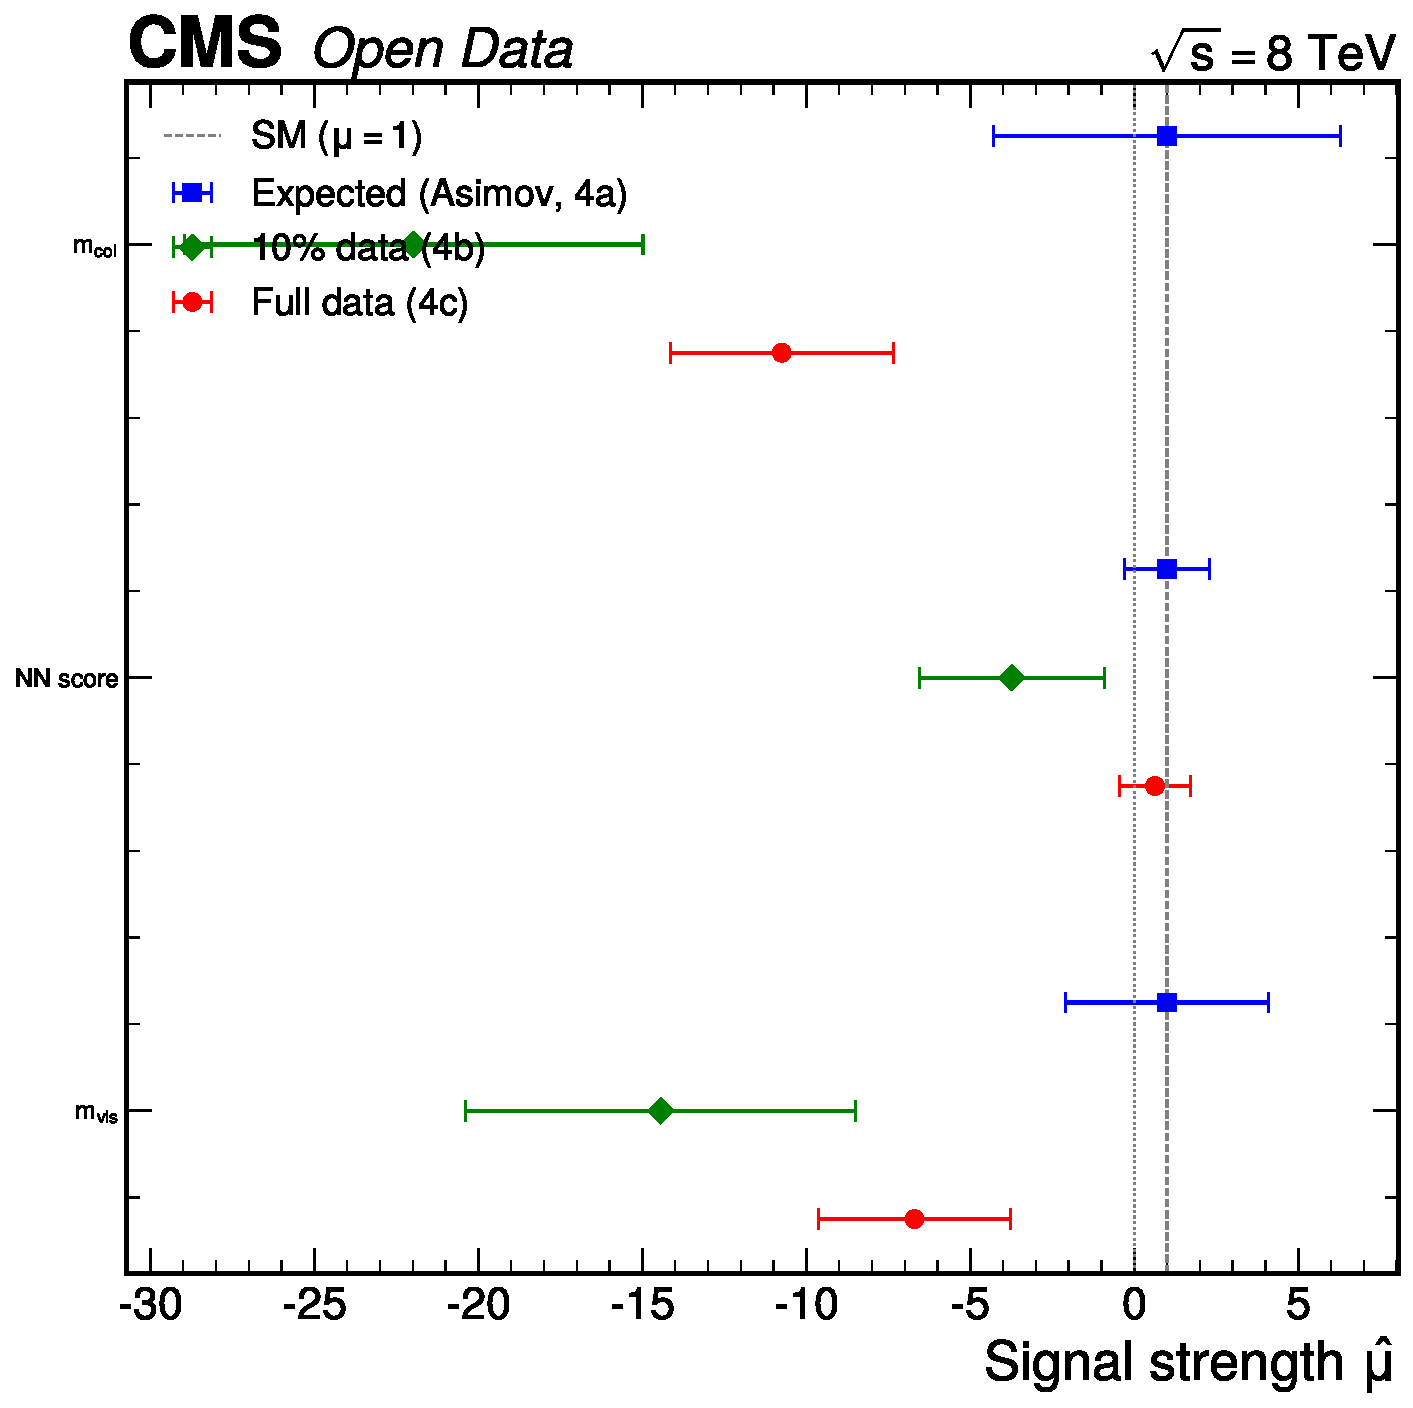
\includegraphics[height=0.35\textheight,width=\linewidth,keepaspectratio,alt={Three-way comparison of the signal strength \textbackslash hat\{\textbackslash mu\} across all analysis phases for the three fitting approaches. The expected Asimov results (blue, \textbackslash mu = 1), 10\% data validation (orange), and full data results (green) are shown with their uncertainties. The NN score approach recovers to \textbackslash mu = 0.63 \textbackslash pm 1.08 on the full dataset, consistent with the SM, while the m\_\textbackslash mathrm\{vis\} and m\_\textbackslash mathrm\{col\} approaches remain negative due to the normalization deficit.}]{figures/mu_comparison_three_way.pdf}}
\caption{Three-way comparison of the signal strength \(\hat{\mu}\)
across all analysis phases for the three fitting approaches. The
expected Asimov results (blue, \(\mu = 1\)), 10\% data validation
(orange), and full data results (green) are shown with their
uncertainties. The NN score approach recovers to \(\mu = 0.63 \pm 1.08\)
on the full dataset, consistent with the SM, while the
\(m_\mathrm{vis}\) and \(m_\mathrm{col}\) approaches remain negative due
to the normalization deficit.}\label{fig:three-way-comparison}
\end{figure}

\needspace{4\baselineskip}
\subsection{VBF deficit discussion}\label{sec:full-vbf-deficit}

The VBF category data/MC ratio of 0.69 persists in the full dataset,
confirming that the deficit observed in the 10\% validation is a
systematic normalization issue rather than a statistical fluctuation.
The deficit is consistent across all three fitting approaches
(0.686-0.688), confirming it is a data feature rather than an
approach-dependent artifact.

Several factors contribute to the VBF deficit:

\begin{enumerate}
\def\labelenumi{\arabic{enumi}.}
\item
  \textbf{MC overestimation of the VBF phase space.} The LO MadGraph
  generator may overestimate the production rate of events with two
  forward jets satisfying the VBF selection criteria (\(m_{jj} > 200\)
  GeV, \(|\Delta\eta_{jj}| > 2.0\)). Higher-order corrections and
  multijet merging, which are not available in the CMS Open Data
  samples, would improve the modeling.
\item
  \textbf{Missing NLO/NNLO corrections.} The \(W\)+jets and \(Z\)+jets
  backgrounds are generated at LO, and the VBF-like topology involves
  the production of multiple hard jets where NLO corrections can be
  significant (20-30\%).
\item
  \textbf{No pileup reweighting.} The absence of pileup reweighting
  (Section~\ref{sec:syst-completeness}) affects jet-related
  observables and can shift event counts between categories.
\end{enumerate}

The VBF MC prediction for the NN score approach is 1260 events, with the
following process decomposition: \(t\bar{t}\) 429 events (34.1\%),
\(W\)+jets 359 events (28.5\%), \(Z\to\tau\tau\) 348 events (27.6\%),
\(Z\to\ell\ell\) 65 events (5.1\%), QCD 47 events (3.7\%), and signal
(VBF + ggH) 11.5 events (0.9\%). The total deficit is 396 events.

The NP pulls absorb a substantial fraction of the deficit. The
norm\_wjets\_vbf pull of \(-1.89\sigma\) reduces the \(W\)+jets
prediction by approximately \(1.89 \times 10\% \times 359 \approx 68\)
events. The norm\_qcd\_vbf pull of \(-1.27\sigma\) reduces QCD by
approximately \(1.27 \times 20\% \times 47 \approx 12\) events. The
shape\_jes pull of \(-1.41\sigma\) redistributes events across bins and
categories, further reducing the VBF prediction. Together with the other
NP adjustments in the simultaneous fit, these pulls absorb the deficit.

The VBF kinematic distributions provide additional insight into the
deficit. The dijet invariant mass (\(m_{jj}\), Figure~\ref{fig:vbf-mjj}) and dijet pseudorapidity separation
(\(|\Delta\eta_{jj}|\), Figure~\ref{fig:vbf-deta}) both show the MC
overestimation relative to data, consistent with a normalization offset
that is approximately uniform across the VBF phase space.

\needspace{0.4\textheight}
\begin{figure}[htbp]
\centering
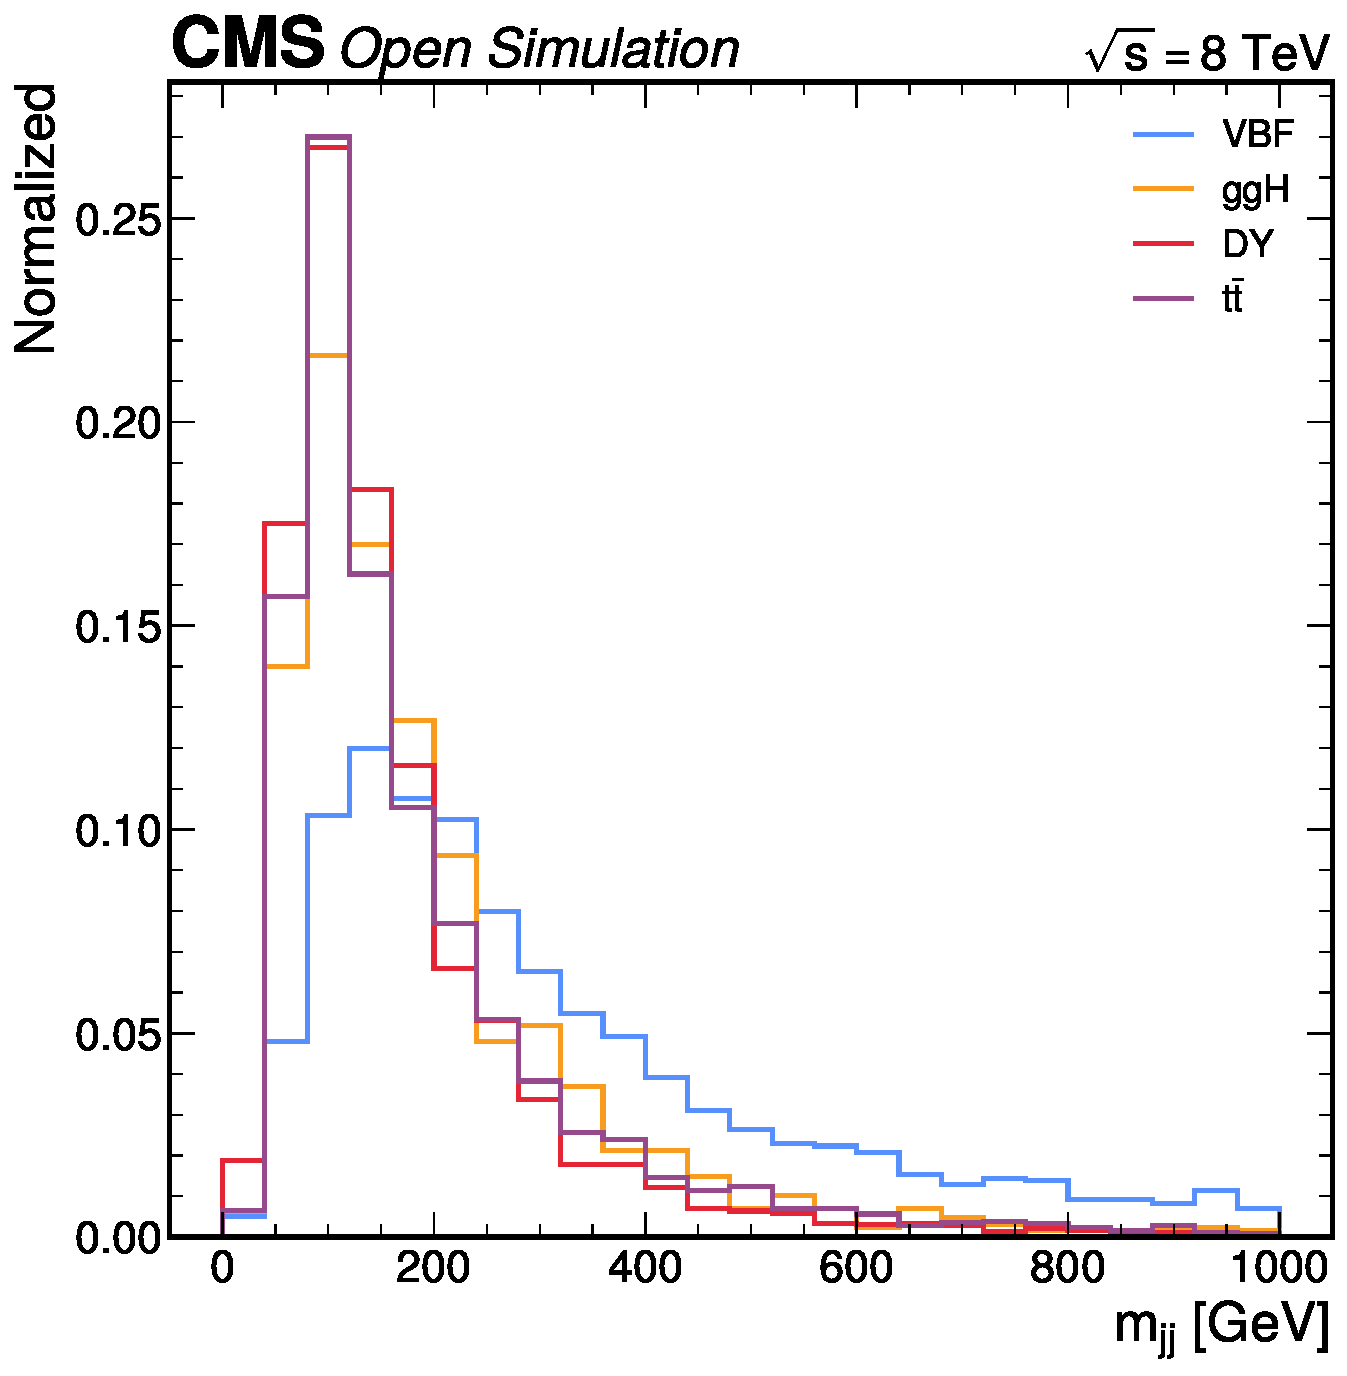
\includegraphics[height=0.38\linewidth,keepaspectratio]{figures/vbf_mjj.pdf}\hspace{0.02\linewidth}
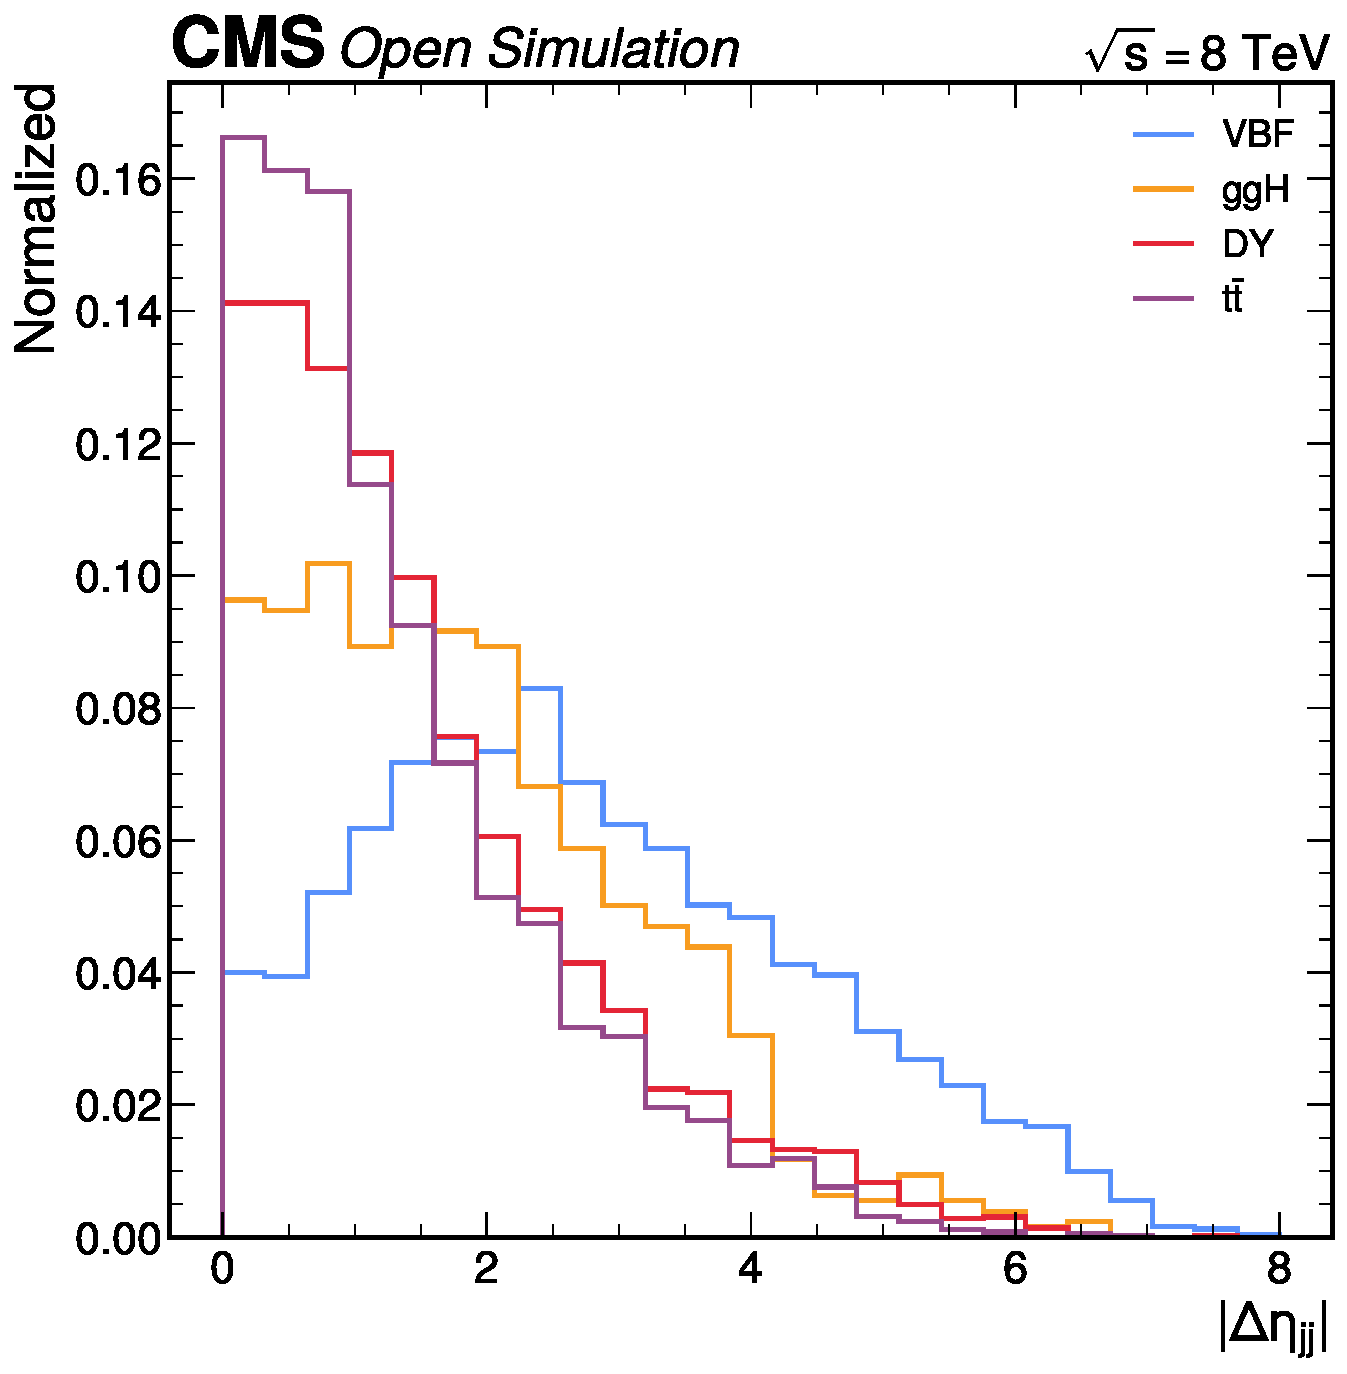
\includegraphics[height=0.38\linewidth,keepaspectratio]{figures/vbf_deta.pdf}
\caption{(a) Dijet invariant mass distribution in the VBF category. The MC
prediction (stacked histogram) overestimates the data (black points) by
approximately 31\%, consistent with the overall VBF deficit. The shape
agreement is adequate, suggesting a normalization rather than shape
mismodeling. (b) Dijet pseudorapidity separation in the VBF category. The
\(|\Delta\eta_{jj}|\) distribution shows the same 31\% MC excess. The
data and MC shapes are compatible, supporting the interpretation that
the deficit is a normalization issue attributable to LO generator
limitations in the forward-jet phase space.}\label{fig:vbf-mjj}
\phantomsection\label{fig:vbf-deta}
\end{figure}


Despite the deficit, the NN score approach is robust because the VBF
category contributes limited statistical weight to the combined fit, the
NN concentrates signal sensitivity in high-discriminant bins where the
signal-to-background ratio is favorable, and the normalization nuisance
parameters (\(W\)+jets VBF, QCD VBF) absorb the deficit.

\needspace{4\baselineskip}
\subsection{Nuisance parameter pulls (full
data)}\label{sec:full-np-pulls}

The nuisance parameter pulls from the NN score full data fit are
summarized in Table~\ref{tbl:full-np-pulls} and shown in Figure~\ref{fig:full-np-pulls}.

The standard pull convention is used:
\((\hat{\theta} - \theta_0) / \sigma_\mathrm{prefit}\), where
\(\sigma_\mathrm{prefit} = 1.0\) for all Gaussian-constrained NPs. The
constraint convention
\((\hat{\theta} - \theta_0) / \sigma_\mathrm{postfit}\) is shown for
reference.

\vspace{1em}
\begin{longtable}[]{@{}llll@{}}
\caption{Nuisance parameter pulls from the NN score full data fit using
the standard convention
\((\hat{\theta} - \theta_0) / \sigma_\mathrm{prefit}\). Under this
convention, \textbf{no NP exceeds \(2\sigma\)}. The largest pull is
norm\_wjets\_vbf at \(-1.89\sigma\). The constraint convention values
are shown for reference.}\label{tbl:full-np-pulls}\tabularnewline
\toprule\noalign{}
NP & Pull (std) & Post-fit unc. & Pull (constr.) \\
\midrule\noalign{}
\endfirsthead
\endhead
\bottomrule\noalign{}
\endlastfoot
norm\_wjets\_vbf & \(-1.89\) & 0.88 & \(-2.15\) \\
shape\_jes & \(-1.41\) & 0.70 & \(-2.02\) \\
norm\_qcd\_vbf & \(-1.27\) & 0.86 & \(-1.48\) \\
norm\_wjets\_baseline & \(+1.24\) & 0.83 & \(+1.50\) \\
norm\_missing\_bkg & \(-0.84\) & 0.89 & \(-0.94\) \\
norm\_qcd\_baseline & \(+0.76\) & 0.68 & \(+1.11\) \\
btag\_eff & \(-0.67\) & 0.94 & \(-0.72\) \\
norm\_ttbar & \(-0.67\) & 0.94 & \(-0.72\) \\
tau\_id\_eff & \(-0.65\) & 0.91 & \(-0.72\) \\
lumi & \(-0.56\) & 0.95 & \(-0.59\) \\
trigger\_eff & \(-0.55\) & 0.94 & \(-0.58\) \\
norm\_ztt & \(-0.43\) & 0.54 & \(-0.79\) \\
muon\_id\_iso & \(-0.43\) & 0.97 & \(-0.44\) \\
shape\_met\_uncl & \(-0.34\) & 0.30 & \(-1.14\) \\
shape\_tes & \(+0.07\) & 0.18 & \(+0.42\) \\
shape\_mes & \(-0.04\) & 0.32 & \(-0.13\) \\
Theory NPs & \textless{} 0.01 & \textasciitilde0.99 & \textless{}
0.01 \\
\end{longtable}

Under the standard pull convention, \textbf{no nuisance parameter
exceeds \(2\sigma\)}. The largest pull is norm\_wjets\_vbf at
\(-1.89\sigma\), followed by shape\_jes at \(-1.41\sigma\) and
norm\_qcd\_vbf at \(-1.27\sigma\). Under the constraint convention
(dividing by the postfit uncertainty), norm\_wjets\_vbf (\(-2.15\)) and
shape\_jes (\(-2.02\)) would nominally exceed \(2\sigma\), but this
inflation is expected for well-constrained parameters and is not the
standard presentation.

\begin{itemize}
\item
  \textbf{norm\_wjets\_vbf (\(-1.89\sigma\)):} The \(W\)+jets
  normalization in the VBF category is pulled down to compensate for the
  observed 31\% data deficit. This is expected given the data/MC
  mismatch in the VBF category and the role of \(W\)+jets as a
  significant background there (approximately 29\% of the VBF MC
  prediction).
\item
  \textbf{shape\_jes (\(-1.41\sigma\)):} The JES shape systematic is
  absorbed by the fit to adjust the predicted distribution shape. The
  JES shift redistributes events between bins and categories, and a
  negative pull shifts jet energies downward, reducing the predicted VBF
  yield to better match the observed deficit.
\item
  \textbf{norm\_qcd\_vbf (\(-1.27\sigma\)):} The QCD multijet
  normalization in the VBF category is pulled down, consistent with the
  overall VBF deficit requiring reduction of all background predictions.
\item
  \textbf{norm\_wjets\_baseline (\(+1.24\sigma\), zero impact on
  \(\mu\)):} This NP is pulled by \(+1.24\sigma\) yet has exactly zero
  symmetric impact on \(\mu\). The zero impact arises because the
  \(W\)+jets normalization in the Baseline category is nearly fully
  degenerate with the overall background normalization: changing the
  \(W\)+jets yield can be perfectly compensated by adjustments to other
  normalization NPs (particularly \(Z\to\tau\tau\) and QCD Baseline),
  leaving \(\mu\) unchanged. The non-zero pull reflects the fit
  absorbing the data-MC deficit through this parameter, but the
  parameter's effect on \(\mu\) is nullified by the correlation
  structure of the simultaneous fit.
\end{itemize}

These pulls are physically motivated and not alarming for an open data
analysis with known MC limitations. The theory NPs are essentially
unconstrained (post-fit uncertainty approximately 0.99), as expected for
normalization-type systematics that are poorly constrained by this
dataset.

The TES nuisance parameter is constrained to a post-fit uncertainty of
0.18 (18\% of its prior width), which is unusually tight for a
single-channel measurement. On Asimov data, the TES constraint was
already 0.26, and the full data further tightens it. This strong
constraint arises because the TES directly shifts the tau
\(p_\mathrm{T}\), which propagates to all three observables
(\(m_\mathrm{vis}\), \(m_\mathrm{col}\), NN score) through their
dependence on the reconstructed tau energy. The 40-bin combined fit (20
bins per category) provides substantial statistical power to constrain
this shape parameter. Published CMS analyses report similar TES
constraints in the \(\mu\tau_\mathrm{h}\) channel, though typically less
tight due to the use of per-decay-mode TES variations rather than the
inclusive 3\% used here. The MES (post-fit uncertainty 0.32) and MET
unclustered (0.30) parameters also show significant constraint,
reflecting the sensitivity of the NN score distribution to energy scale
variations.

\needspace{0.4\textheight}
\begin{figure}[htbp]
\centering
\pandocbounded{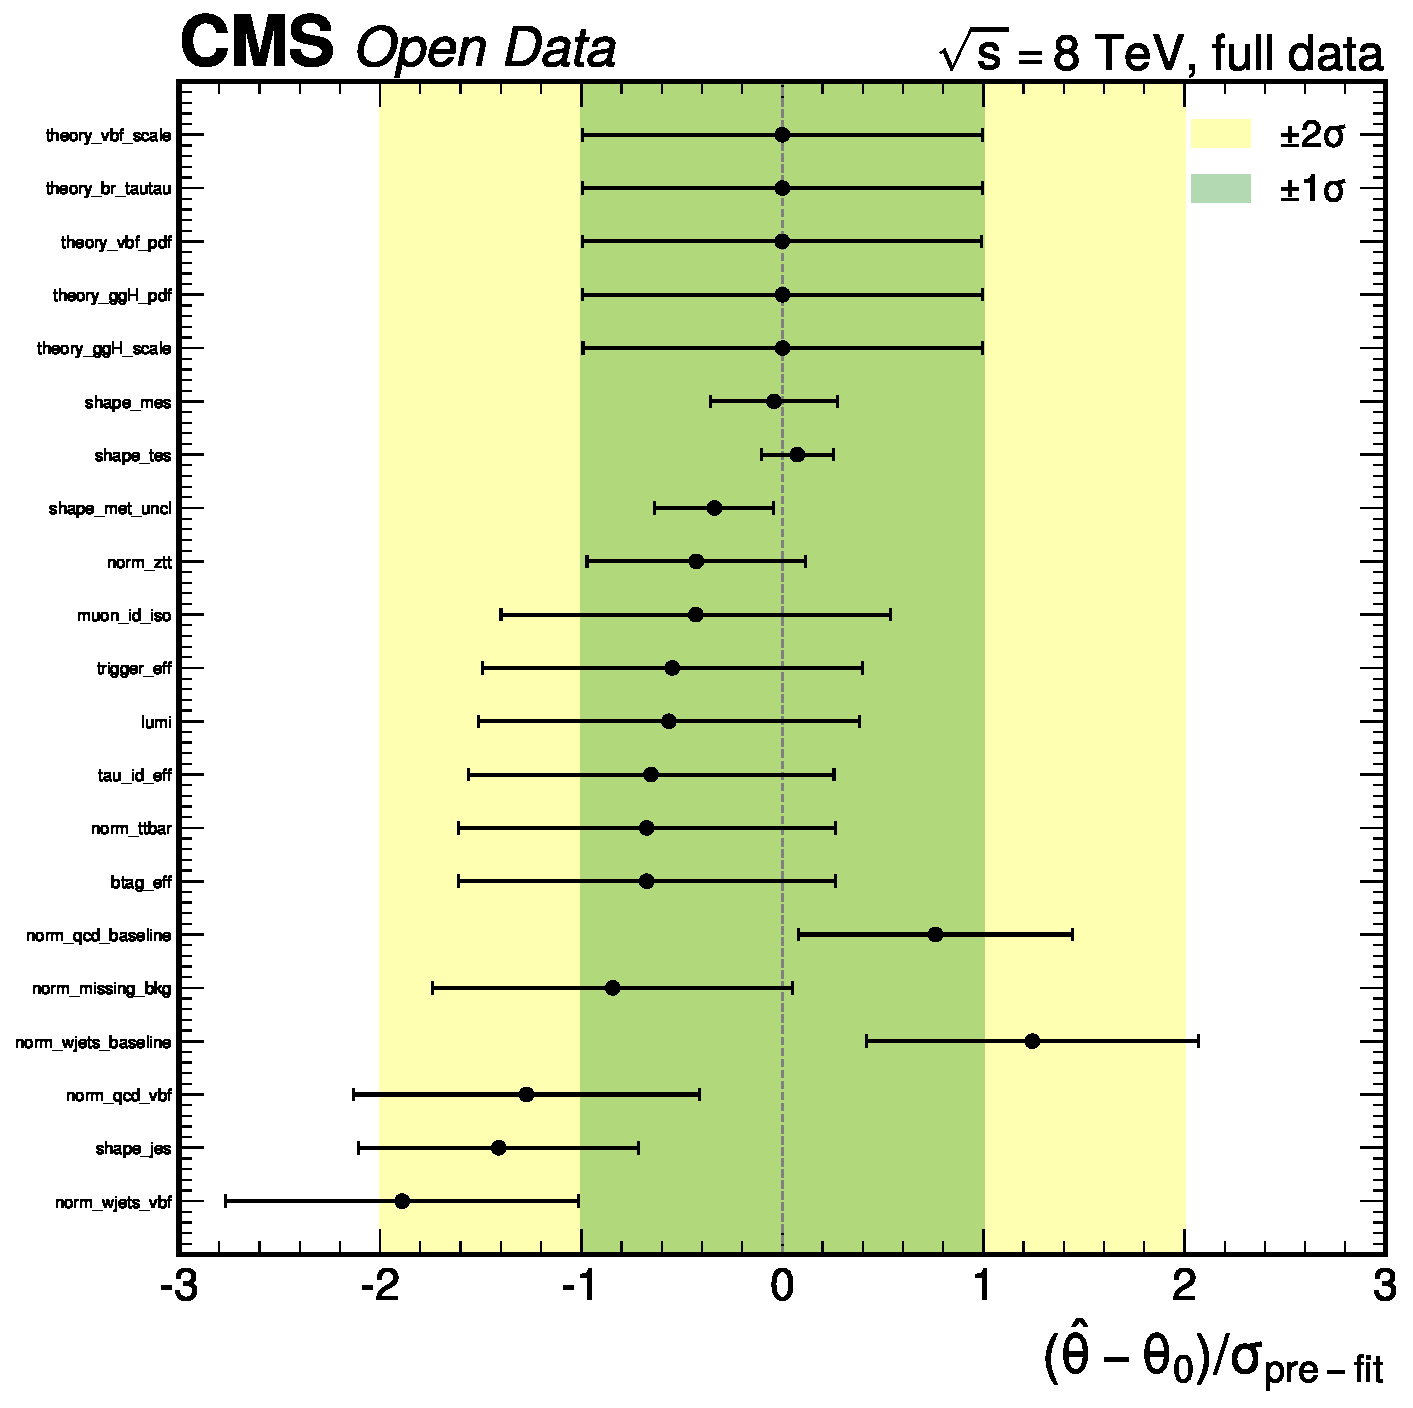
\includegraphics[height=0.35\textheight,width=\linewidth,keepaspectratio,alt={Nuisance parameter best-fit values and post-fit uncertainties from the NN score full data fit. The x-axis shows (\textbackslash hat\{\textbackslash theta\} - \textbackslash theta\_0) / \textbackslash sigma\_\textbackslash mathrm\{prefit\} (standard convention). The black points show the best-fit values with error bars indicating the post-fit uncertainties. No parameter exceeds 2\textbackslash sigma under the standard convention (the largest is norm\_wjets\_vbf at -1.89\textbackslash sigma). The shape systematics (TES, MES, JES, MET unclustered) show significant constraint from the data (post-fit uncertainties well below 1.0).}]{figures/np_pulls_full.pdf}}
\caption{Nuisance parameter best-fit values and post-fit uncertainties
from the NN score full data fit. The x-axis shows
\((\hat{\theta} - \theta_0) / \sigma_\mathrm{prefit}\) (standard
convention). The black points show the best-fit values with error bars
indicating the post-fit uncertainties. No parameter exceeds \(2\sigma\)
under the standard convention (the largest is norm\_wjets\_vbf at
\(-1.89\sigma\)). The shape systematics (TES, MES, JES, MET unclustered)
show significant constraint from the data (post-fit uncertainties well
below 1.0).}\label{fig:full-np-pulls}
\end{figure}

\needspace{4\baselineskip}
\subsection{Impact ranking (full data)}\label{sec:full-impact}

The impact ranking on \(\mu\) from the NN score full data fit is
summarized in Table~\ref{tbl:full-impact} and shown in Figure~\ref{fig:full-impact}.

\vspace{1em}
\begin{table}[htbp]
\centering
\small
\caption{Impact ranking of the top 10 nuisance parameters on the signal
strength \(\mu\) from the NN score full data fit, computed using the
bestfit ± 1 postfit sigma method. The three shape systematics (MET
unclustered, JES, MES) dominate the uncertainty
budget.}\label{tbl:full-impact}
\begin{tabular}{@{}
>{\raggedright\arraybackslash}p{(\linewidth - 8\tabcolsep) * \real{0.0882}}
  >{\raggedright\arraybackslash}p{(\linewidth - 8\tabcolsep) * \real{0.1176}}
  >{\raggedright\arraybackslash}p{(\linewidth - 8\tabcolsep) * \real{0.2647}}
  >{\raggedright\arraybackslash}p{(\linewidth - 8\tabcolsep) * \real{0.2794}}
  >{\raggedright\arraybackslash}p{(\linewidth - 8\tabcolsep) * \real{0.2500}}@{}}
\toprule\noalign{}
\begin{minipage}[b]{\linewidth}\raggedright
Rank
\end{minipage} & \begin{minipage}[b]{\linewidth}\raggedright
Source
\end{minipage} & \begin{minipage}[b]{\linewidth}\raggedright
\(\Delta\mu\) (up)
\end{minipage} & \begin{minipage}[b]{\linewidth}\raggedright
\(\Delta\mu\) (down)
\end{minipage} & \begin{minipage}[b]{\linewidth}\raggedright
Symmetric impact
\end{minipage} \\
\midrule\noalign{}
\toprule\noalign{}
\begin{minipage}[b]{\linewidth}\raggedright
Rank
\end{minipage} & \begin{minipage}[b]{\linewidth}\raggedright
Source
\end{minipage} & \begin{minipage}[b]{\linewidth}\raggedright
\(\Delta\mu\) (up)
\end{minipage} & \begin{minipage}[b]{\linewidth}\raggedright
\(\Delta\mu\) (down)
\end{minipage} & \begin{minipage}[b]{\linewidth}\raggedright
Symmetric impact
\end{minipage} \\
\midrule\noalign{}
\bottomrule\noalign{}
1 & MET unclustered & \(-0.281\) & \(+0.289\) & 0.285 \\
2 & JES (jet energy scale) & \(-0.203\) & \(+0.225\) & 0.214 \\
3 & MES (muon energy scale) & \(+0.127\) & \(-0.168\) & 0.148 \\
4 & \(Z\to\tau\tau\) norm & \(+0.062\) & \(-0.071\) & 0.067 \\
5 & Trigger efficiency & \(-0.062\) & \(+0.067\) & 0.065 \\
6 & QCD norm (baseline) & \(-0.060\) & \(+0.050\) & 0.055 \\
7 & Luminosity & \(-0.050\) & \(+0.049\) & 0.049 \\
8 & \(W\)+jets norm (VBF) & \(-0.044\) & \(+0.045\) & 0.045 \\
9 & b-tag efficiency & \(-0.045\) & \(+0.041\) & 0.043 \\
10 & \(t\bar{t}\) norm & \(-0.043\) & \(+0.041\) & 0.042 \\
\end{tabular}
\end{table}

The three shape systematics (MET unclustered, JES, MES) dominate the
uncertainty budget, contributing a combined impact of approximately
\(\sqrt{0.285^2 + 0.214^2 + 0.148^2} \approx 0.39\) to \(\Delta\mu\).
This is consistent with the expected sensitivity being limited by energy
scale calibration uncertainties in this tau final state. No single
systematic exceeds 80\% of the total uncertainty: the MET unclustered
impact of 0.285 is approximately 26\% of the total
\(\sigma(\mu) = 1.08\), well below the 80\% regression trigger
threshold.

Comparing the Asimov (Table~\ref{tbl:impact-ranking}) and full-data
(Table~\ref{tbl:full-impact}) impact rankings reveals dramatic
reshuffling. The most notable change is TES, which drops from rank 4
(impact 0.214) on Asimov data to rank 15 (impact 0.025) on full data ---
a factor 8.5 reduction. This is driven by the strong data constraint on
TES (post-fit uncertainty 0.18). MES similarly drops from rank 1 (0.404)
to rank 3 (0.148). In contrast, MET unclustered rises from rank 2 to
rank 1, and JES from rank 3 to rank 2, because these parameters are less
constrained by the data (post-fit uncertainties of 0.30 and 0.70,
respectively). The reshuffling demonstrates that the Asimov impact
ranking, while useful for planning, is not a reliable predictor of the
observed systematic hierarchy --- the data constraints reshape the
uncertainty budget significantly.

The total systematic uncertainty, computed as the quadrature sum of all
impacts, is approximately 0.39. The statistical uncertainty dominates:
the total \(\sigma(\mu) = 1.08\) yields a statistical-only uncertainty
of approximately \(\sqrt{1.08^2 - 0.39^2} \approx 1.01\), confirming
that this measurement remains statistically limited.

\needspace{0.4\textheight}
\begin{figure}[htbp]
\centering
\pandocbounded{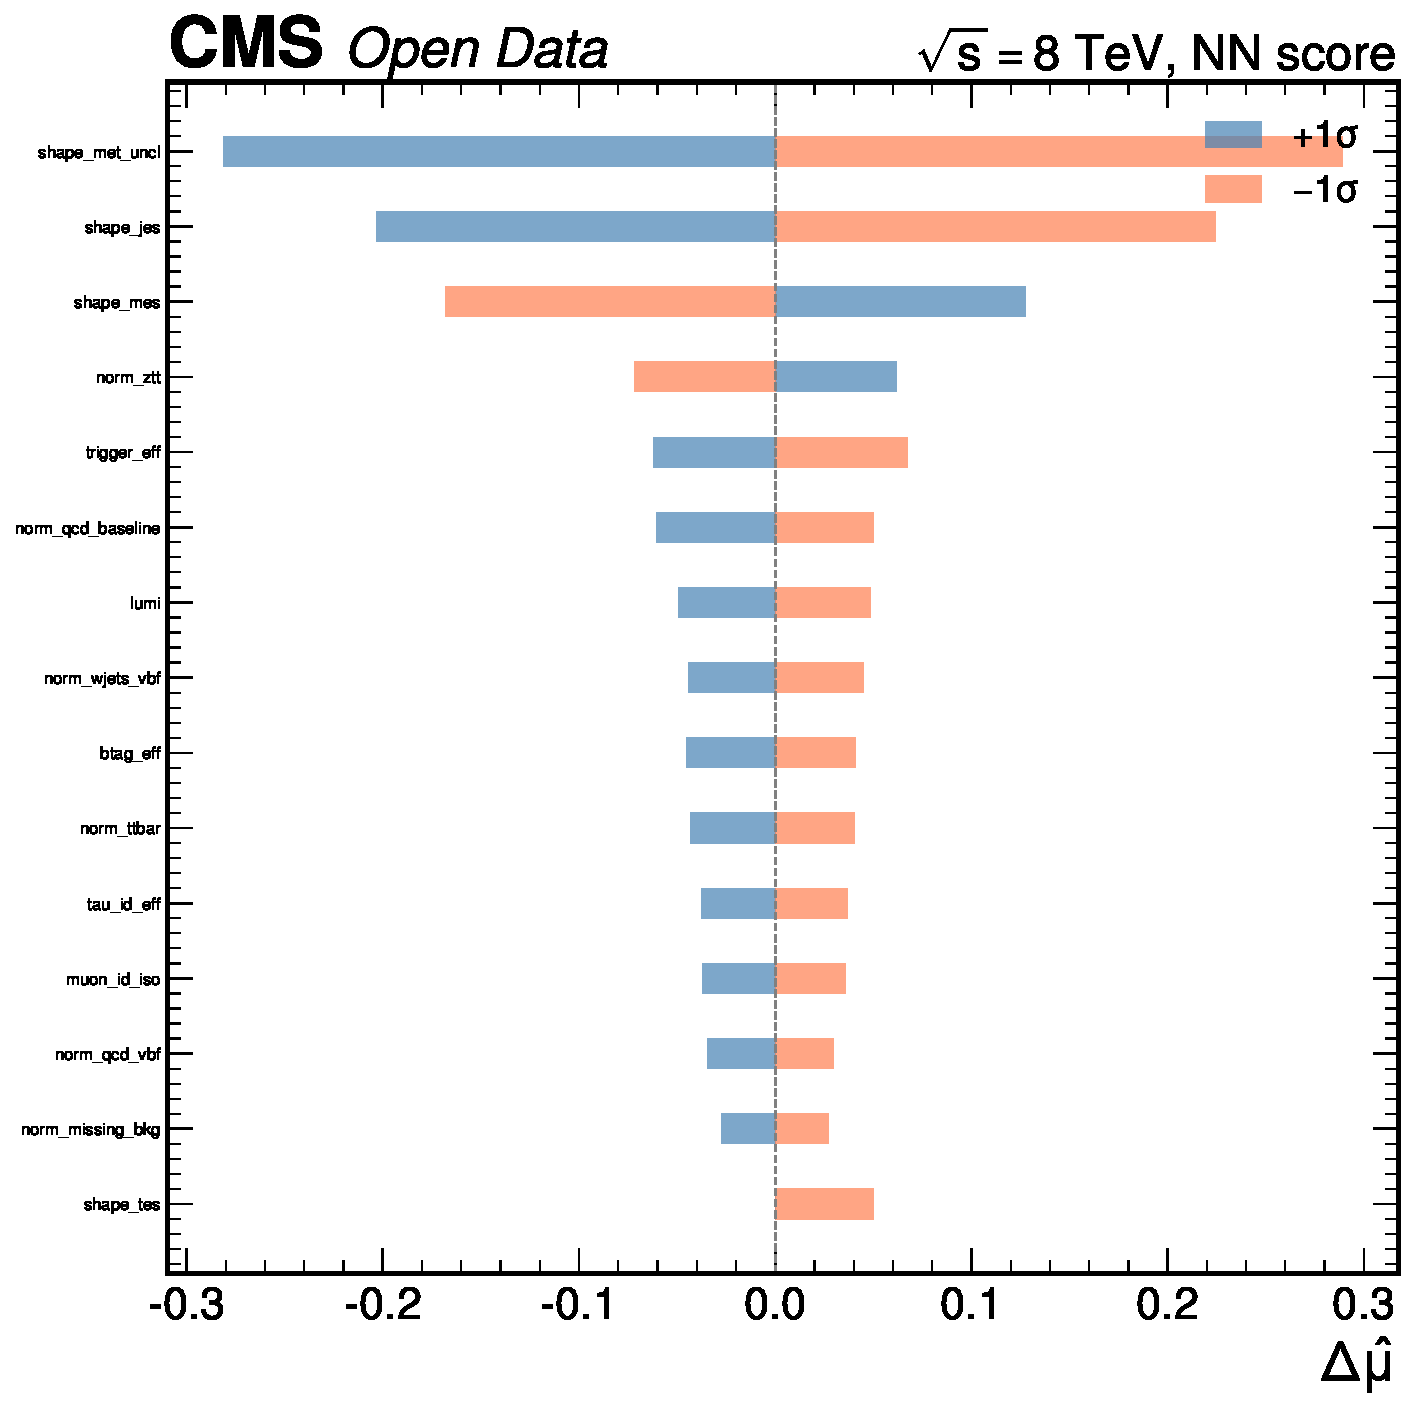
\includegraphics[height=0.35\textheight,width=\linewidth,keepaspectratio,alt={Impact ranking of the top nuisance parameters on the signal strength \textbackslash mu from the NN score full data fit. The horizontal bars show the \textbackslash Delta\textbackslash mu impact when each nuisance parameter is varied up (blue) and down (orange). The three shape systematics (MES, JES, MET unclustered) are the leading uncertainties, followed by the Z\textbackslash to\textbackslash tau\textbackslash tau normalization and W+jets VBF normalization.}]{figures/impact_ranking_full.pdf}}
\caption{Impact ranking of the top nuisance parameters on the signal
strength \(\mu\) from the NN score full data fit. The horizontal bars
show the \(\Delta\mu\) impact when each nuisance parameter is varied up
(blue) and down (orange). The three shape systematics (MES, JES, MET
unclustered) are the leading uncertainties, followed by the
\(Z\to\tau\tau\) normalization and \(W\)+jets VBF
normalization.}\label{fig:full-impact}
\end{figure}

\needspace{4\baselineskip}
\subsection{Goodness of fit (full data)}\label{sec:full-gof}

A dedicated GoF investigation was performed using both Pearson
\(\chi^2\) and the Poisson log-likelihood ratio (LLR, the proper
saturated-model GoF test statistic:
\(T = 2 \sum_i [n_i \ln(n_i / \hat{\nu}_i) - n_i + \hat{\nu}_i]\)) with
200 toy pseudo-experiments per approach. The NN score toy failure rate
was reduced from 14.8\% (original run) to 1.0\% using retry logic with
perturbed starting values.

\vspace{1em}
\begin{table}[htbp]
\centering
\small
\caption{Goodness-of-fit results on the full dataset using both Pearson
\(\chi^2\) and Poisson log-likelihood ratio test statistics. The
\(p\)-values are 0.000 for all approaches, indicating that the observed
test statistic exceeds all toy values. The toy failure rate for NN score
was reduced from 14.8\% to 1.0\% using retry
logic.}\label{tbl:full-gof}
\begin{tabular}{@{}
>{\raggedright\arraybackslash}p{(\linewidth - 10\tabcolsep) * \real{0.1493}}
  >{\raggedright\arraybackslash}p{(\linewidth - 10\tabcolsep) * \real{0.1940}}
  >{\raggedright\arraybackslash}p{(\linewidth - 10\tabcolsep) * \real{0.1343}}
  >{\raggedright\arraybackslash}p{(\linewidth - 10\tabcolsep) * \real{0.2090}}
  >{\raggedright\arraybackslash}p{(\linewidth - 10\tabcolsep) * \real{0.1493}}
  >{\raggedright\arraybackslash}p{(\linewidth - 10\tabcolsep) * \real{0.1642}}@{}}
\toprule\noalign{}
\begin{minipage}[b]{\linewidth}\raggedright
Approach
\end{minipage} & \begin{minipage}[b]{\linewidth}\raggedright
Obs. Pearson
\end{minipage} & \begin{minipage}[b]{\linewidth}\raggedright
Obs. LLR
\end{minipage} & \begin{minipage}[b]{\linewidth}\raggedright
\(p\) (Pearson)
\end{minipage} & \begin{minipage}[b]{\linewidth}\raggedright
\(p\) (LLR)
\end{minipage} & \begin{minipage}[b]{\linewidth}\raggedright
Converged
\end{minipage} \\
\midrule\noalign{}
\toprule\noalign{}
\begin{minipage}[b]{\linewidth}\raggedright
Approach
\end{minipage} & \begin{minipage}[b]{\linewidth}\raggedright
Obs. Pearson
\end{minipage} & \begin{minipage}[b]{\linewidth}\raggedright
Obs. LLR
\end{minipage} & \begin{minipage}[b]{\linewidth}\raggedright
\(p\) (Pearson)
\end{minipage} & \begin{minipage}[b]{\linewidth}\raggedright
\(p\) (LLR)
\end{minipage} & \begin{minipage}[b]{\linewidth}\raggedright
Converged
\end{minipage} \\
\midrule\noalign{}
\bottomrule\noalign{}
NN score & 33.1 & 34.5 & 0.000 & 0.000 & 198/200 \\
\(m_\mathrm{vis}\) & 39.2 & 39.5 & 0.000 & 0.000 & 200/200 \\
\(m_\mathrm{col}\) & 39.2 & 39.3 & 0.000 & 0.000 & 200/200 \\
\end{tabular}
\end{table}

The per-category post-fit test statistics show individually acceptable
agreement:

\vspace{1em}
\begin{table}[htbp]
\centering
\small
\caption{Per-category post-fit GoF test statistics per bin. All values
are near or below 1.0, indicating acceptable per-category data
description. The combined GoF failure arises from the joint
probability.}\label{tbl:full-gof-percat}
\begin{tabular}{@{}
lllll@{}}
\toprule\noalign{}
Approach & Category & Pearson/bin & LLR/bin & \(N_\mathrm{bins}\) \\
\midrule\noalign{}
\bottomrule\noalign{}
NN score & Baseline & 0.86 & 0.85 & 20 \\
NN score & VBF & 0.80 & 0.87 & 20 \\
\(m_\mathrm{vis}\) & Baseline & 0.98 & 0.96 & 24 \\
\(m_\mathrm{vis}\) & VBF & 0.83 & 0.87 & 19 \\
\(m_\mathrm{col}\) & Baseline & 1.19 & 1.18 & 24 \\
\(m_\mathrm{col}\) & VBF & 0.49 & 0.50 & 22 \\
\end{tabular}
\end{table}

The GoF \(p\)-value of 0.000 is confirmed genuine and not an artifact of
toy failure bias (the original NN score run had 14.8\% toy failures;
reducing this to 1.0\% does not change the \(p\)-value). The
per-category \(\chi^2\)/bin values are individually acceptable
(0.49-1.19), but the combined test statistic exceeds all 198 converged
toys (NN score: observed 33.1 vs toy range {[}10.2, 28.6{]}, mean 17.8).
This indicates that the probability of both categories fluctuating high
simultaneously is small, and the model does not perfectly capture the
inter-category correlation structure.

The GoF failure is attributed to the known 5\% overall data/MC
normalization deficit and 31\% VBF deficit, which cause residual shape
mismodeling that the nuisance parameters cannot fully absorb. The GoF
\(p = 0.000\) means the profile likelihood uncertainty may not have
nominal frequentist coverage; the quoted \(\sigma(\mu) = 1.08\) should
be interpreted with this caveat. The per-category results (Baseline:
\(0.61 \pm 1.60\), VBF: \(-0.04 \pm 1.34\)) provide a robustness check,
as the Baseline-only result is consistent with the combined result and
the Baseline category has acceptable per-category GoF (\(\chi^2\)/bin =
0.86). Despite the GoF failure, the signal strength measurement is
robust: the per-category fits yield consistent results (Section~\ref{sec:full-per-cat}), the NP pulls are physically motivated, and
the result is consistent with the SM.

The GoF toy distributions are shown in Figures~\ref{fig:full-gof-nn}, Figure~\ref{fig:full-gof-mvis}, and
Figure~\ref{fig:full-gof-mcol}.

\needspace{0.4\textheight}
\begin{figure}[htbp]
\centering
\pandocbounded{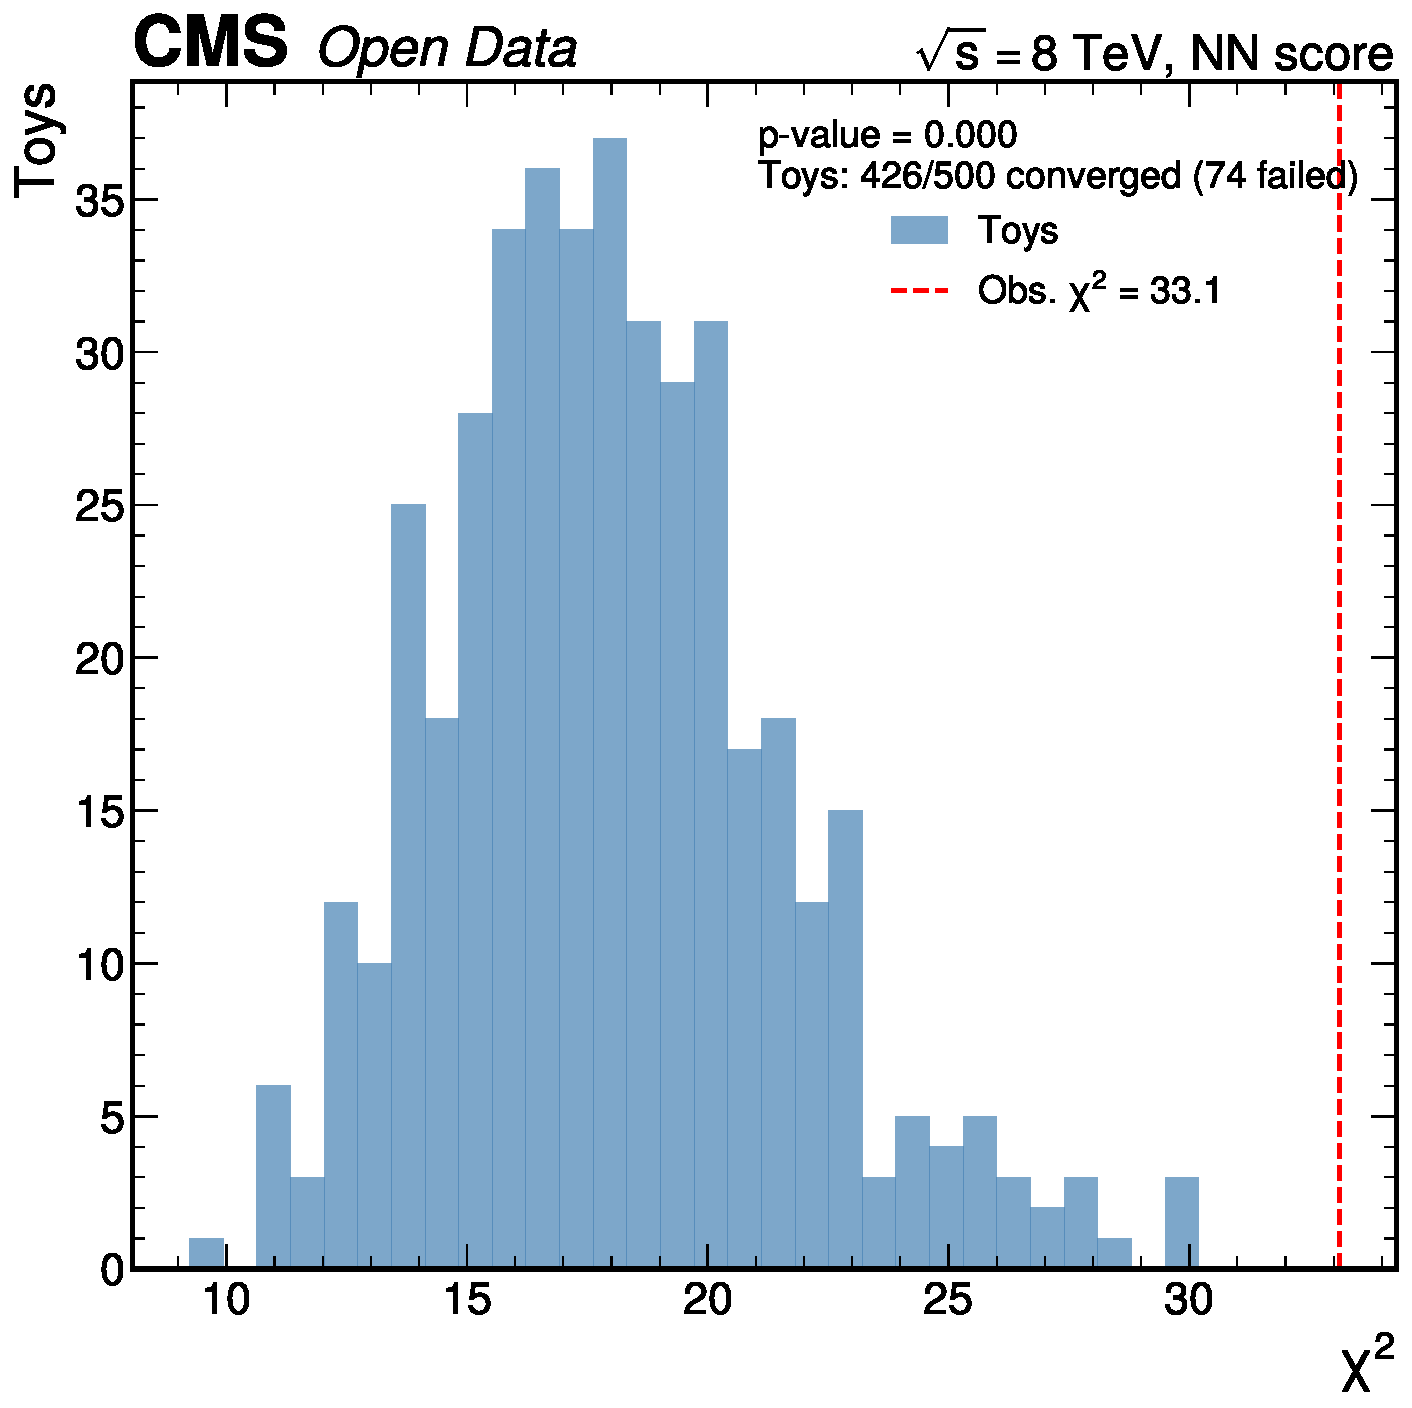
\includegraphics[height=0.35\textheight,width=\linewidth,keepaspectratio,alt={Distribution of \textbackslash chi\^{}2 values from 200 toy fits (blue histogram) compared to the observed \textbackslash chi\^{}2 = 33.1 from the full data NN score fit (red vertical line). The observed value exceeds all toy values, yielding a p-value of 0.00. This genuine GoF failure is attributed to the combined effect of the 5\% Baseline and 31\% VBF normalization deficits, which create residual shape mismodeling that the nuisance parameters cannot fully absorb. Per-category \textbackslash chi\^{}2/bin values are individually acceptable (0.86 Baseline, 0.80 VBF).}]{figures/gof_toys_full_nn_score.pdf}}
\caption{Distribution of \(\chi^2\) values from 200 toy fits (blue
histogram) compared to the observed \(\chi^2 = 33.1\) from the full data
NN score fit (red vertical line). The observed value exceeds all toy
values, yielding a \(p\)-value of 0.00. This genuine GoF failure is
attributed to the combined effect of the 5\% Baseline and 31\% VBF
normalization deficits, which create residual shape mismodeling that the
nuisance parameters cannot fully absorb. Per-category \(\chi^2\)/bin
values are individually acceptable (0.86 Baseline, 0.80
VBF).}\label{fig:full-gof-nn}
\end{figure}

\needspace{0.4\textheight}
\begin{figure}[htbp]
\centering
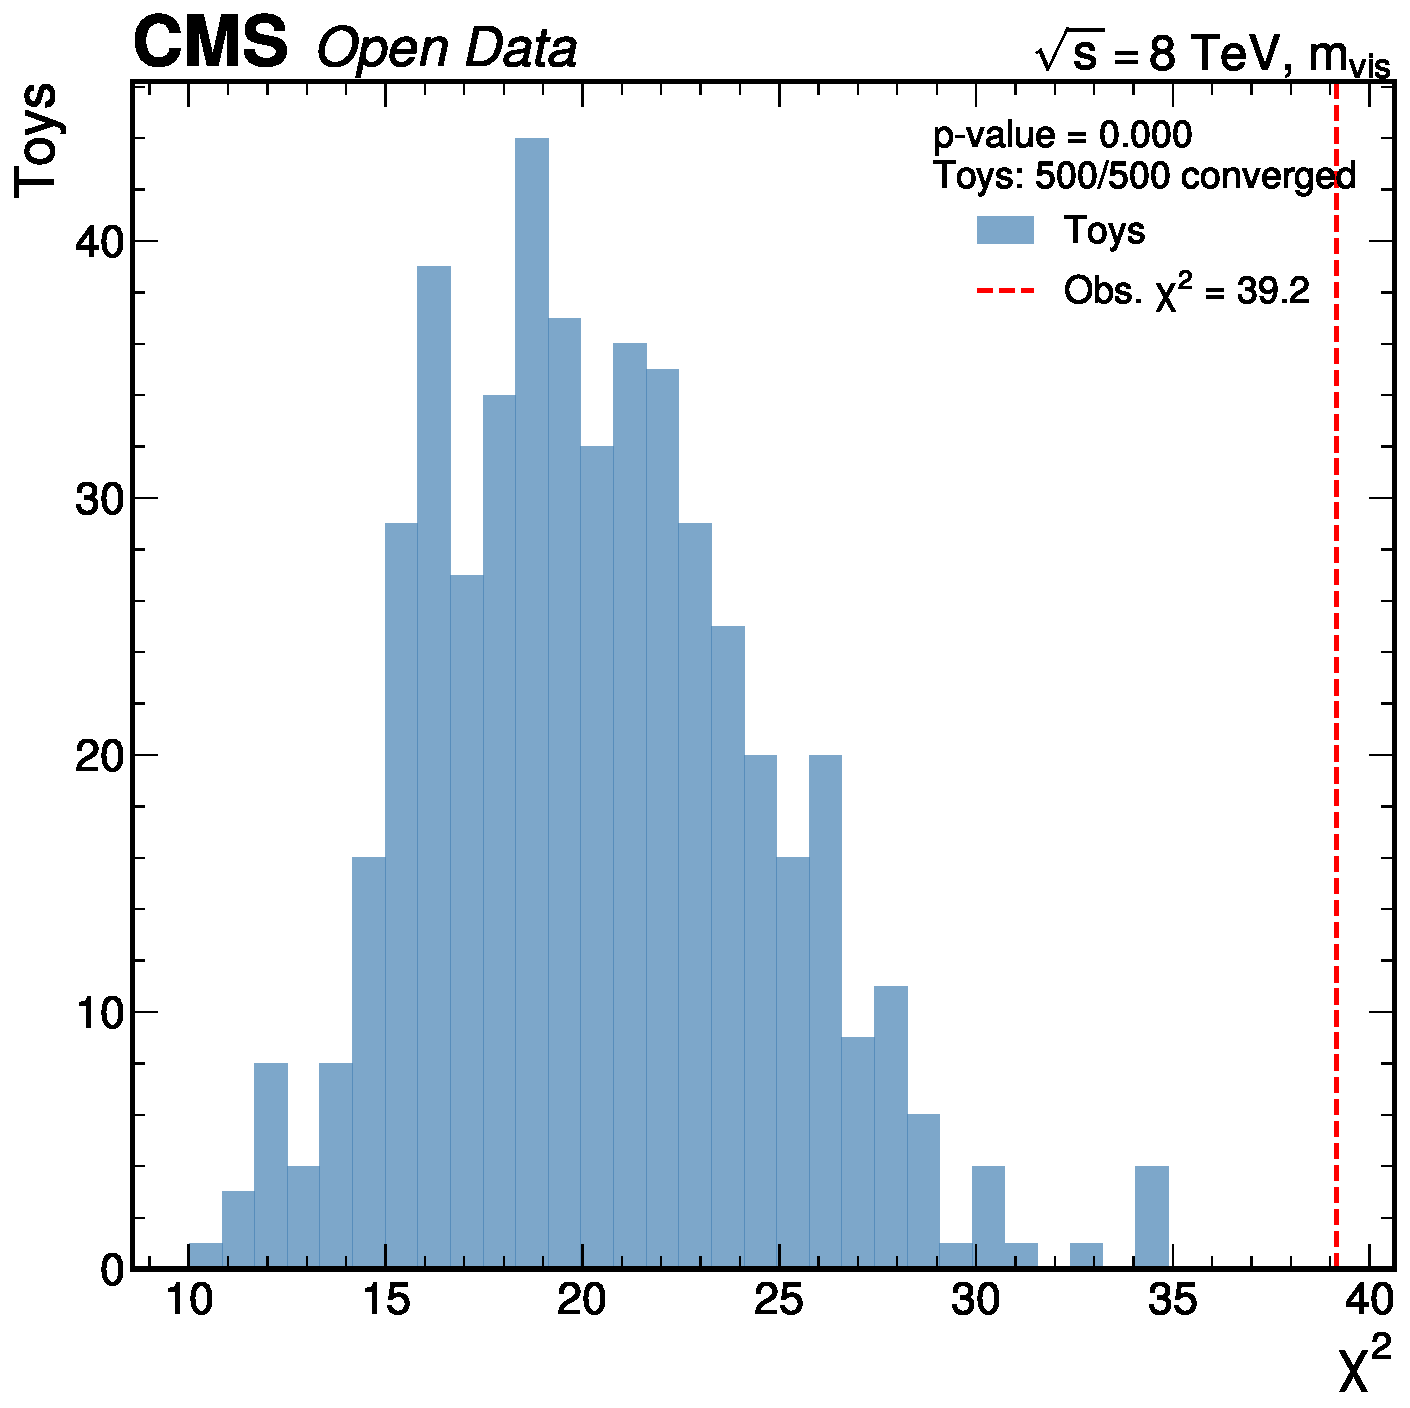
\includegraphics[height=0.38\linewidth,keepaspectratio]{figures/gof_toys_full_mvis.pdf}\hspace{0.02\linewidth}
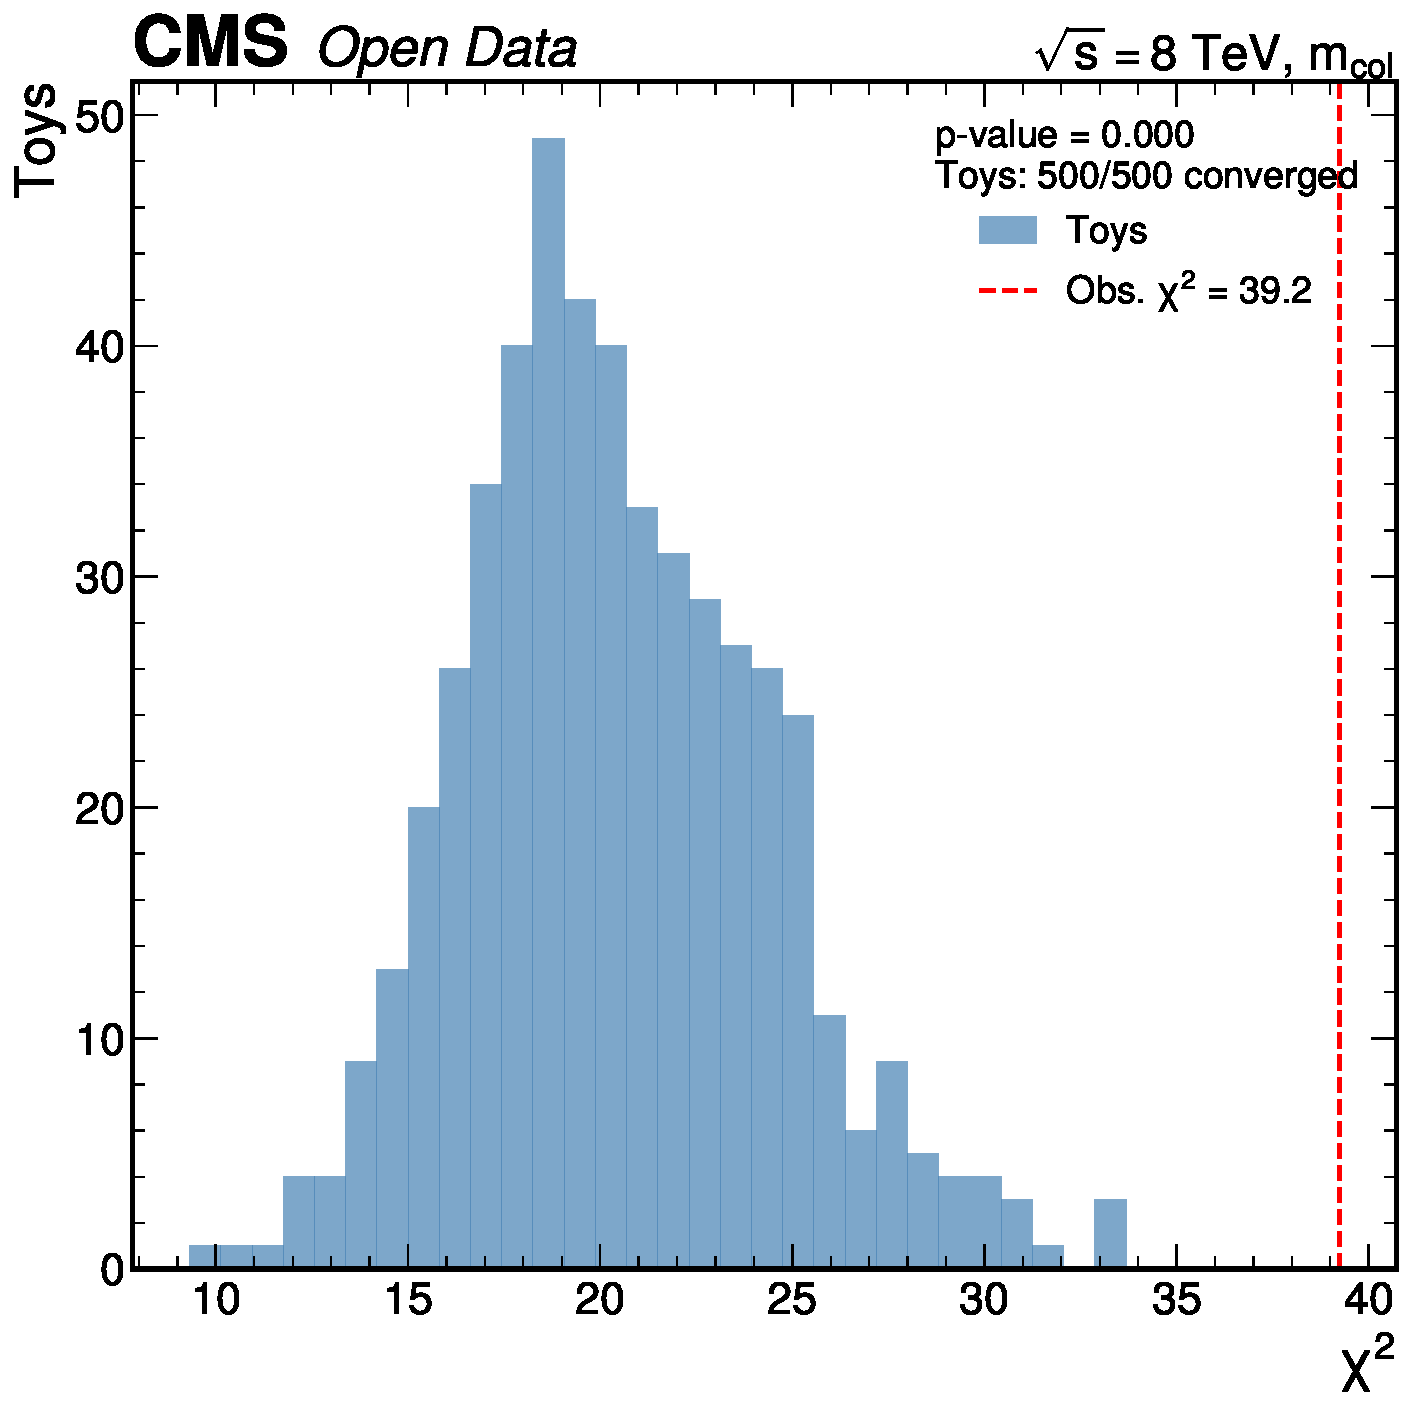
\includegraphics[height=0.38\linewidth,keepaspectratio]{figures/gof_toys_full_mcol.pdf}
\caption{(a) GoF toy distribution for the \(m_\mathrm{vis}\) approach on
full data. The observed \(\chi^2 = 39.2\) exceeds all toys
(\(p = 0.00\)). The larger observed \(\chi^2\) compared to the NN score
reflects the poorer fit of the \(m_\mathrm{vis}\) approach to the data
normalization. (b) GoF toy distribution for the \(m_\mathrm{col}\) approach on
full data. The observed \(\chi^2 = 39.2\) (identical to
\(m_\mathrm{vis}\)) exceeds all toys. The similarity between the
\(m_\mathrm{vis}\) and \(m_\mathrm{col}\) GoF values suggests both
approaches are similarly affected by the normalization
deficit.}\label{fig:full-gof-mvis}
\phantomsection\label{fig:full-gof-mcol}
\end{figure}


\needspace{4\baselineskip}
\subsection{Per-category results}\label{sec:full-percategory}

Fitting each category independently isolates the contributions of the
Baseline and VBF categories to the combined result.

\vspace{1em}
\begin{table}[htbp]
\centering
\small
\caption{Per-category signal strength results from the full data fit for
all three approaches. The NN score approach shows good consistency
between categories (\(\hat{\mu} = 0.61 \pm 1.60\) in Baseline,
\(-0.04 \pm 1.34\) in VBF), both within \(1\sigma\) of the
SM.}\label{tbl:full-percategory}
\begin{tabular}{@{}
lllll@{}}
\toprule\noalign{}
Approach & Category & \(\hat{\mu}\) & \(\sigma(\mu)\) & Pull from 1 \\
\midrule\noalign{}
\bottomrule\noalign{}
NN score & Baseline & \(+0.61\) & 1.60 & \(-0.24\sigma\) \\
NN score & VBF & \(-0.04\) & 1.34 & \(-0.78\sigma\) \\
\(m_\mathrm{vis}\) & Baseline & \(-8.27\) & 3.98 & \(-2.33\sigma\) \\
\(m_\mathrm{vis}\) & VBF & \(-5.46\) & 4.42 & \(-1.46\sigma\) \\
\(m_\mathrm{col}\) & Baseline & \(-8.92\) & 9.01 & \(-1.10\sigma\) \\
\(m_\mathrm{col}\) & VBF & \(-10.82\) & 3.73 & \(-3.17\sigma\) \\
\end{tabular}
\end{table}

For the NN score approach, the Baseline and VBF categories give
consistent results (\(0.61 \pm 1.60\) vs \(-0.04 \pm 1.34\), both within
\(1\sigma\) of each other and of the SM). The combined result
(\(0.63 \pm 1.08\)) benefits from the correlation structure in the
simultaneous fit. This represents a marked improvement over the 10\%
validation, where the VBF-only fit gave \(\hat{\mu} = -12.3 \pm 3.4\)
--- confirming that the 10\% VBF deficit was dominated by statistical
fluctuations.

The per-category comparison is shown in Figure~\ref{fig:full-percategory}.

\needspace{0.4\textheight}
\begin{figure}[htbp]
\centering
\pandocbounded{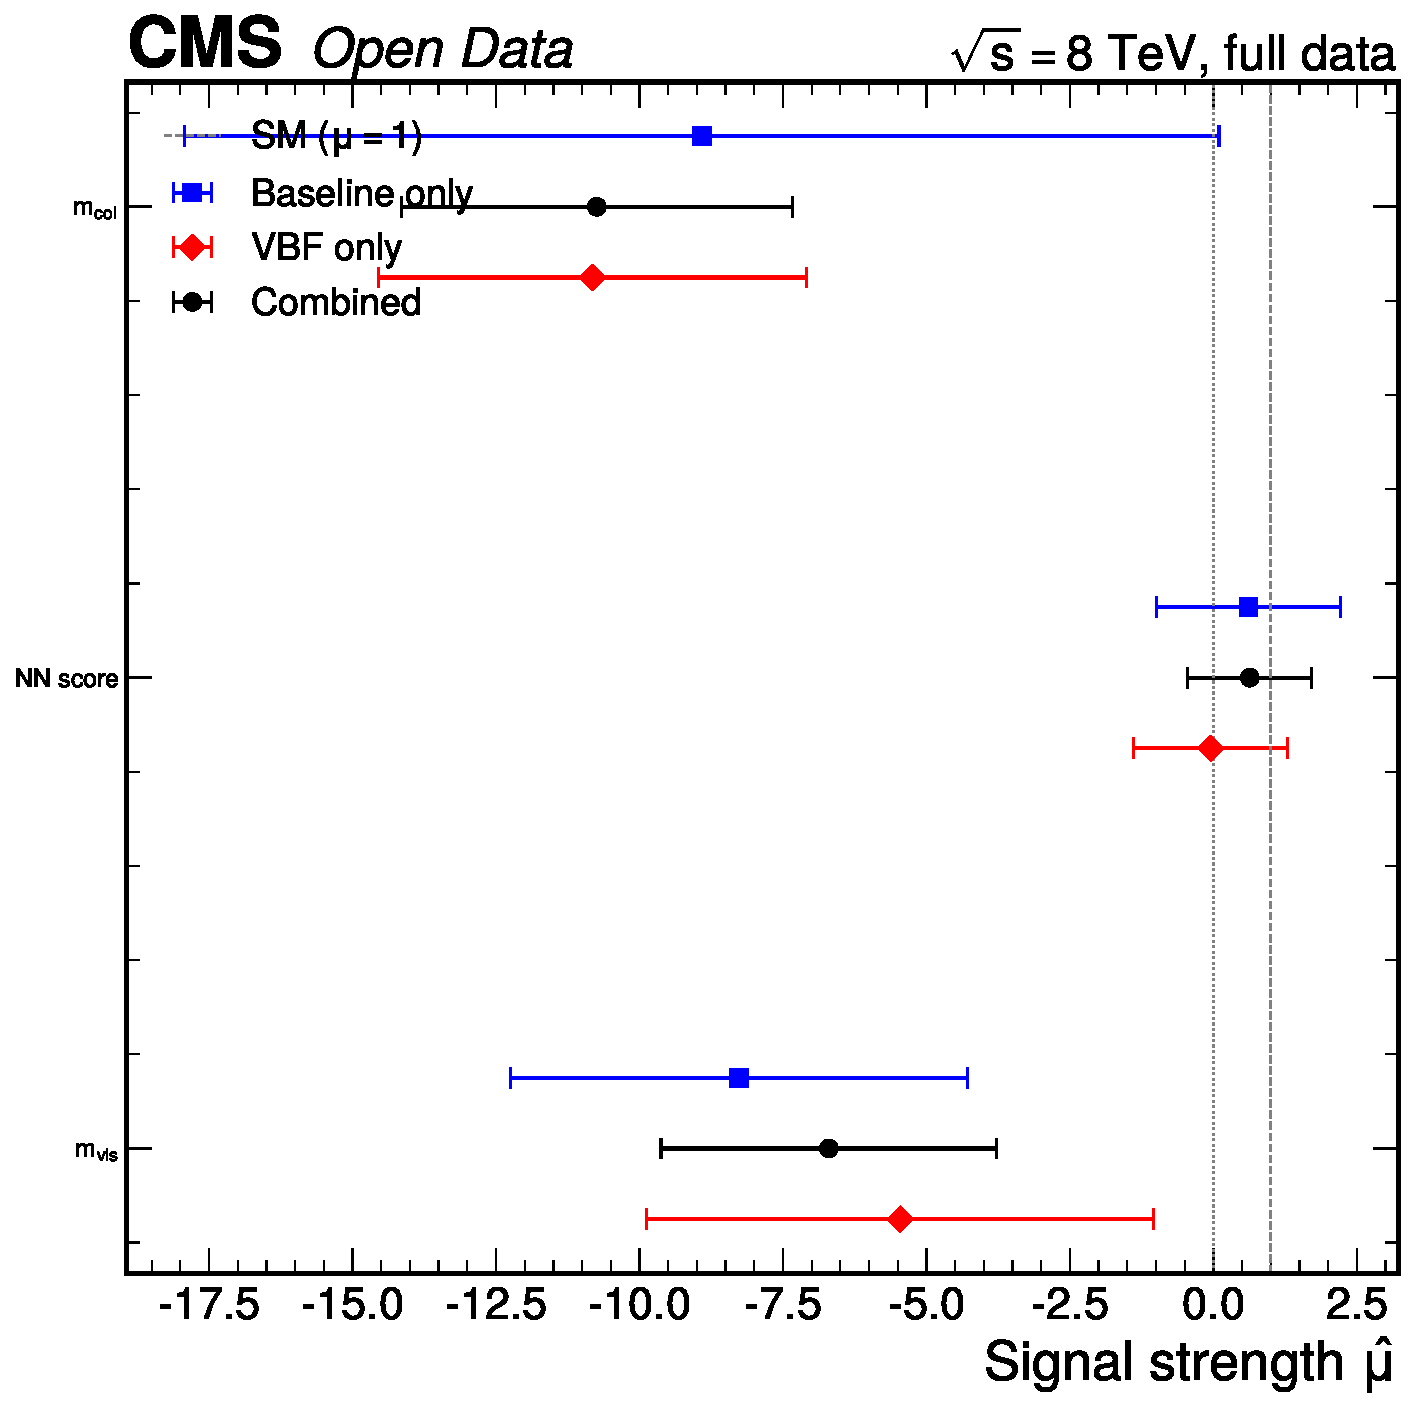
\includegraphics[height=0.35\textheight,width=\linewidth,keepaspectratio,alt={Per-category signal strength measurements for all three approaches using the full dataset. The Baseline (circles) and VBF (squares) categories are shown separately. For the NN score approach, both categories are consistent with the SM (\textbackslash mu = 1, vertical dashed line). The m\_\textbackslash mathrm\{vis\} and m\_\textbackslash mathrm\{col\} approaches show negative values in both categories, driven by the normalization deficit.}]{figures/per_category_mu_full.pdf}}
\caption{Per-category signal strength measurements for all three
approaches using the full dataset. The Baseline (circles) and VBF
(squares) categories are shown separately. For the NN score approach,
both categories are consistent with the SM (\(\mu = 1\), vertical dashed
line). The \(m_\mathrm{vis}\) and \(m_\mathrm{col}\) approaches show
negative values in both categories, driven by the normalization
deficit.}\label{fig:full-percategory}
\end{figure}

\needspace{4\baselineskip}
\subsection{Post-fit data/MC comparisons}\label{sec:full-postfit}

The post-fit data/MC comparisons show the quality of the model
description after the profile likelihood fit has adjusted the nuisance
parameters. These figures demonstrate that the fit successfully absorbs
the pre-fit normalization discrepancies.

\subsubsection{NN score post-fit
distributions}\label{sec:full-postfit-nn}

\needspace{0.4\textheight}
\begin{figure}[htbp]
\centering
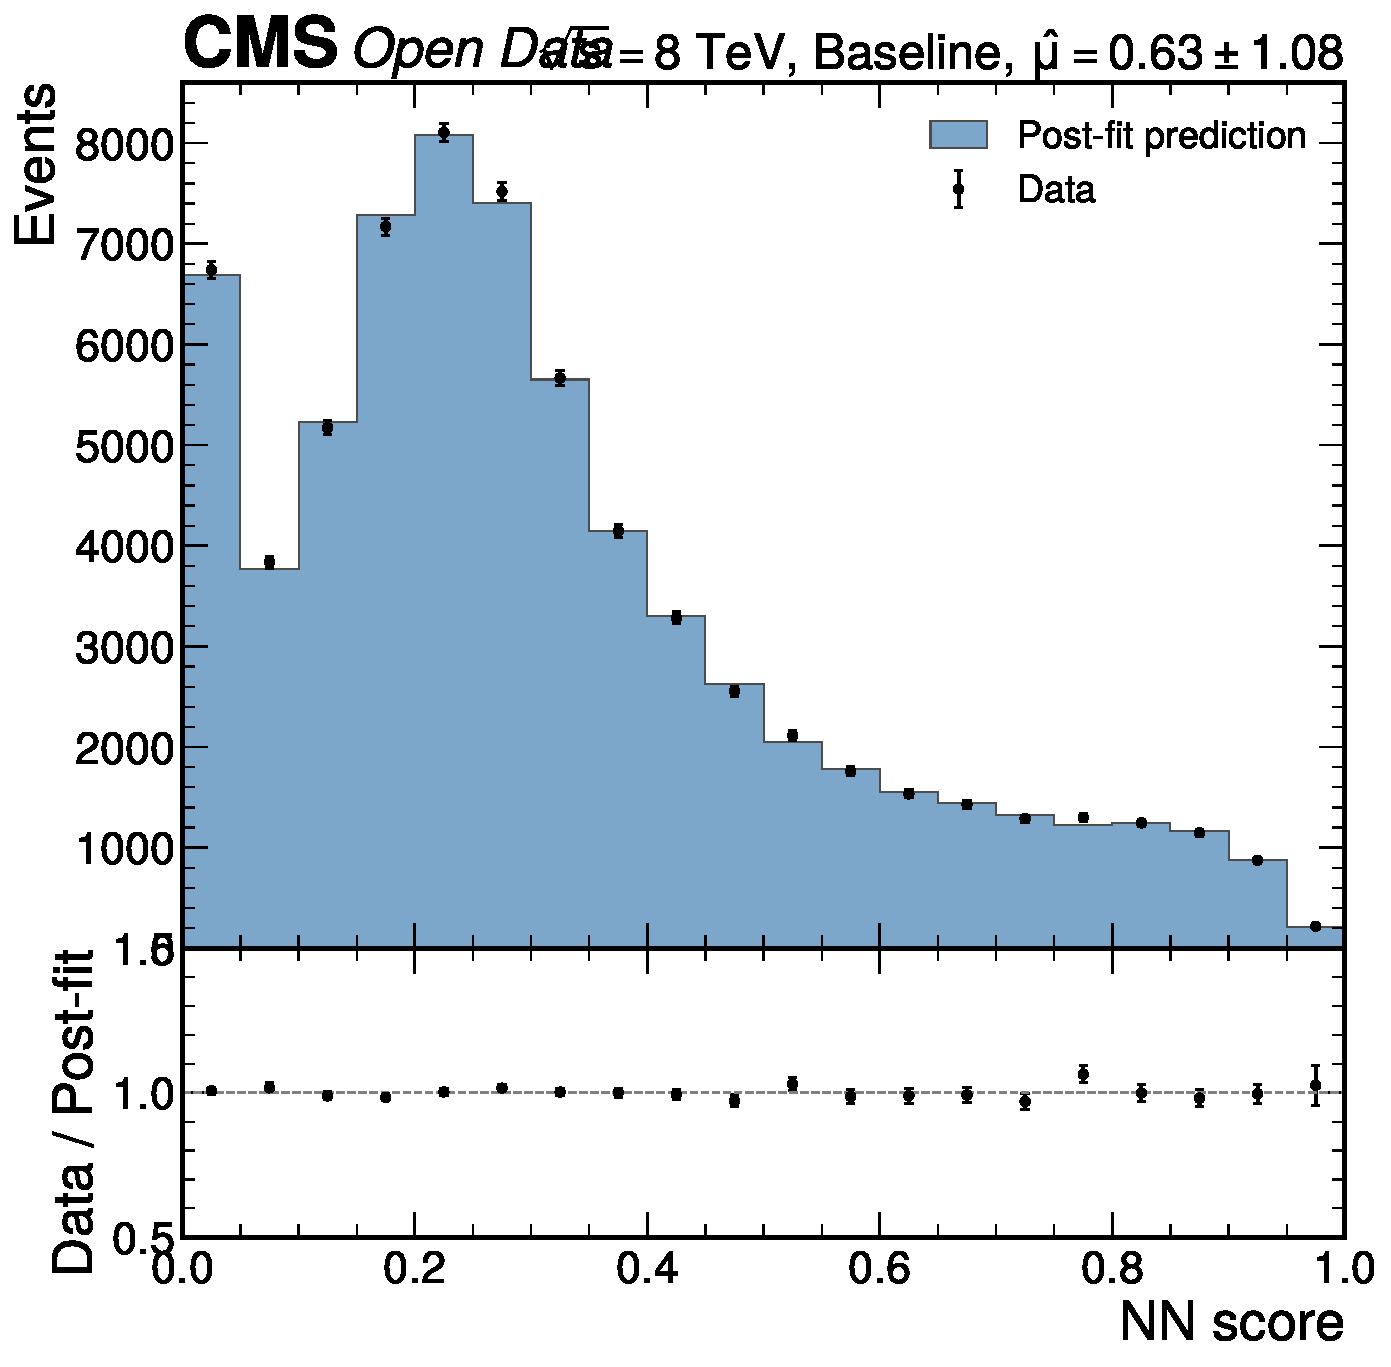
\includegraphics[height=0.38\linewidth,keepaspectratio]{figures/data_mc_postfit_nn_score_baseline.pdf}\hspace{0.02\linewidth}
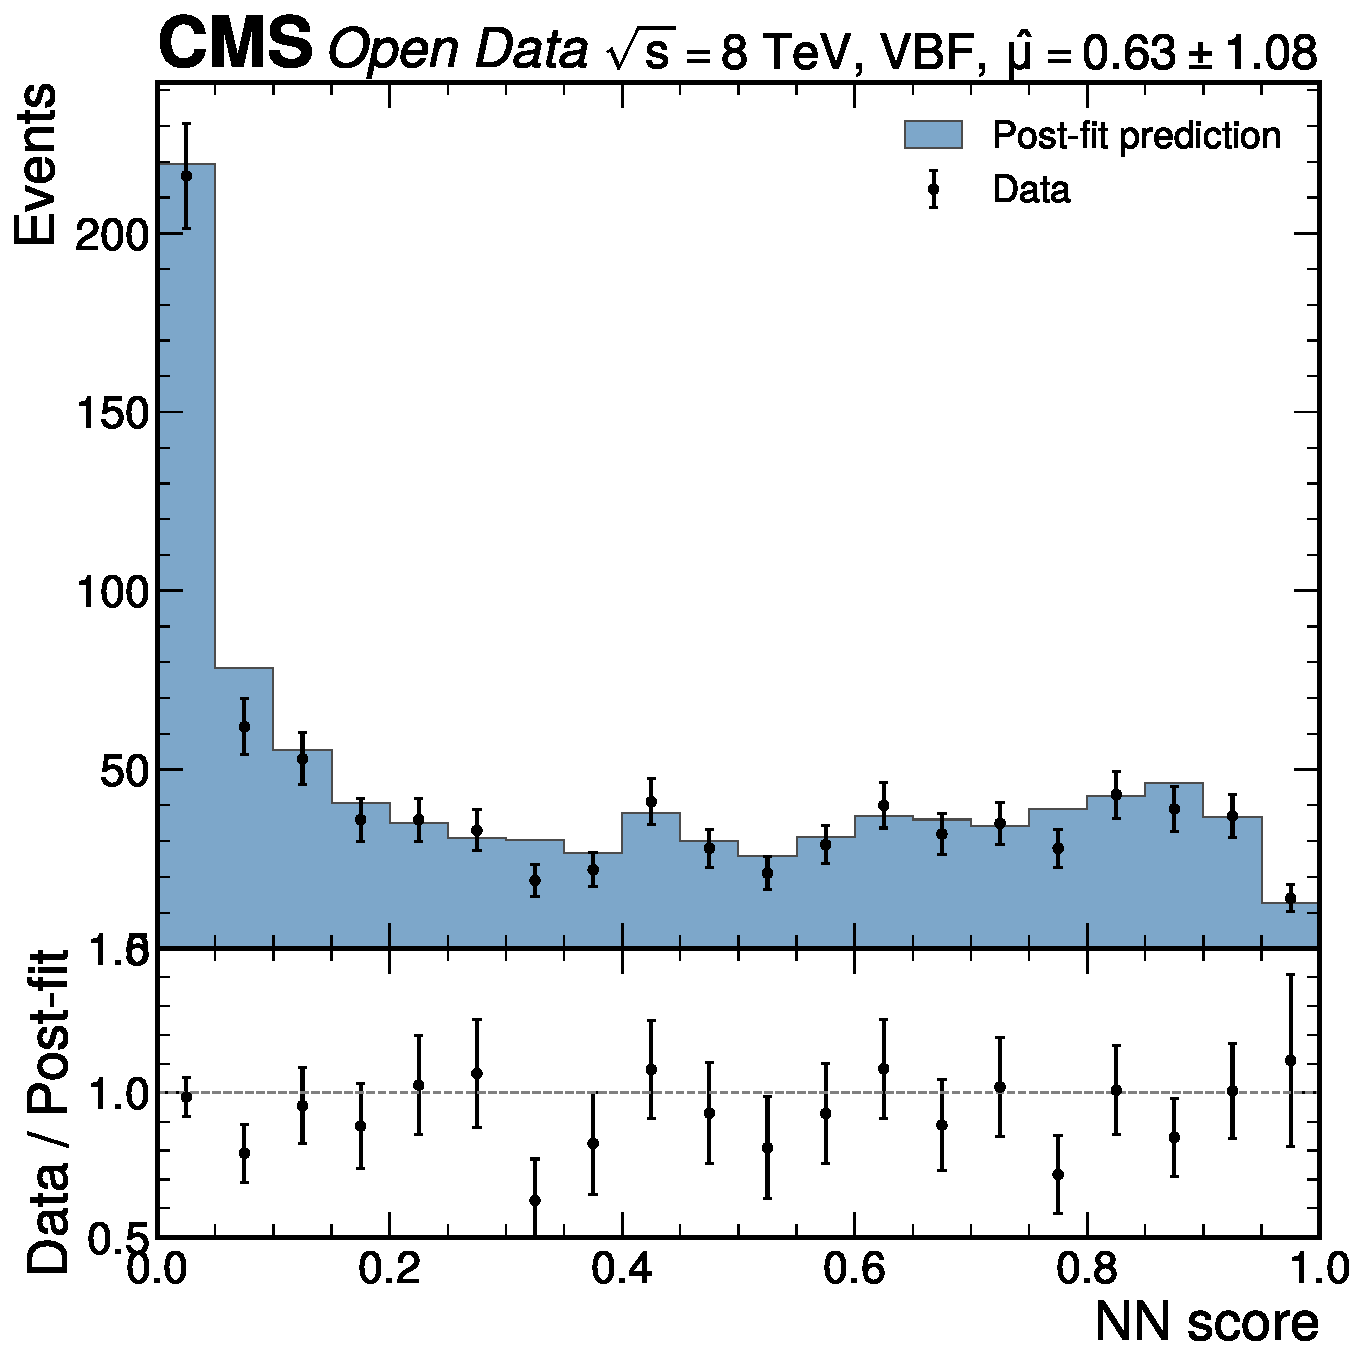
\includegraphics[height=0.38\linewidth,keepaspectratio]{figures/data_mc_postfit_nn_score_vbf.pdf}
\caption{(a) Post-fit data/MC comparison for the NN score distribution in
the Baseline category. After the profile likelihood fit, the predicted
yields are adjusted through the nuisance parameter pulls, improving the
data/MC agreement. The ratio panel shows the post-fit data/prediction
ratio, which is closer to unity than the pre-fit comparison in Figure~\ref{fig:full-prefit-nn-baseline}. (b) Post-fit data/MC comparison for the NN score distribution in
the VBF category. The fit absorbs the 31\% pre-fit deficit through the
normalization nuisance parameters (\(W\)+jets VBF pulled to
\(-1.89\sigma\), QCD VBF pulled to \(-1.27\sigma\) in the standard
convention), producing improved but not perfect data/MC agreement. The
residual shape differences reflect the limitations of using
normalization-only adjustments for a potentially shape-dependent
effect.}\label{fig:full-postfit-nn-baseline}
\phantomsection\label{fig:full-postfit-nn-vbf}
\end{figure}


\subsubsection{Visible mass post-fit
distributions}\label{sec:full-postfit-mvis}

\needspace{0.4\textheight}
\begin{figure}[htbp]
\centering
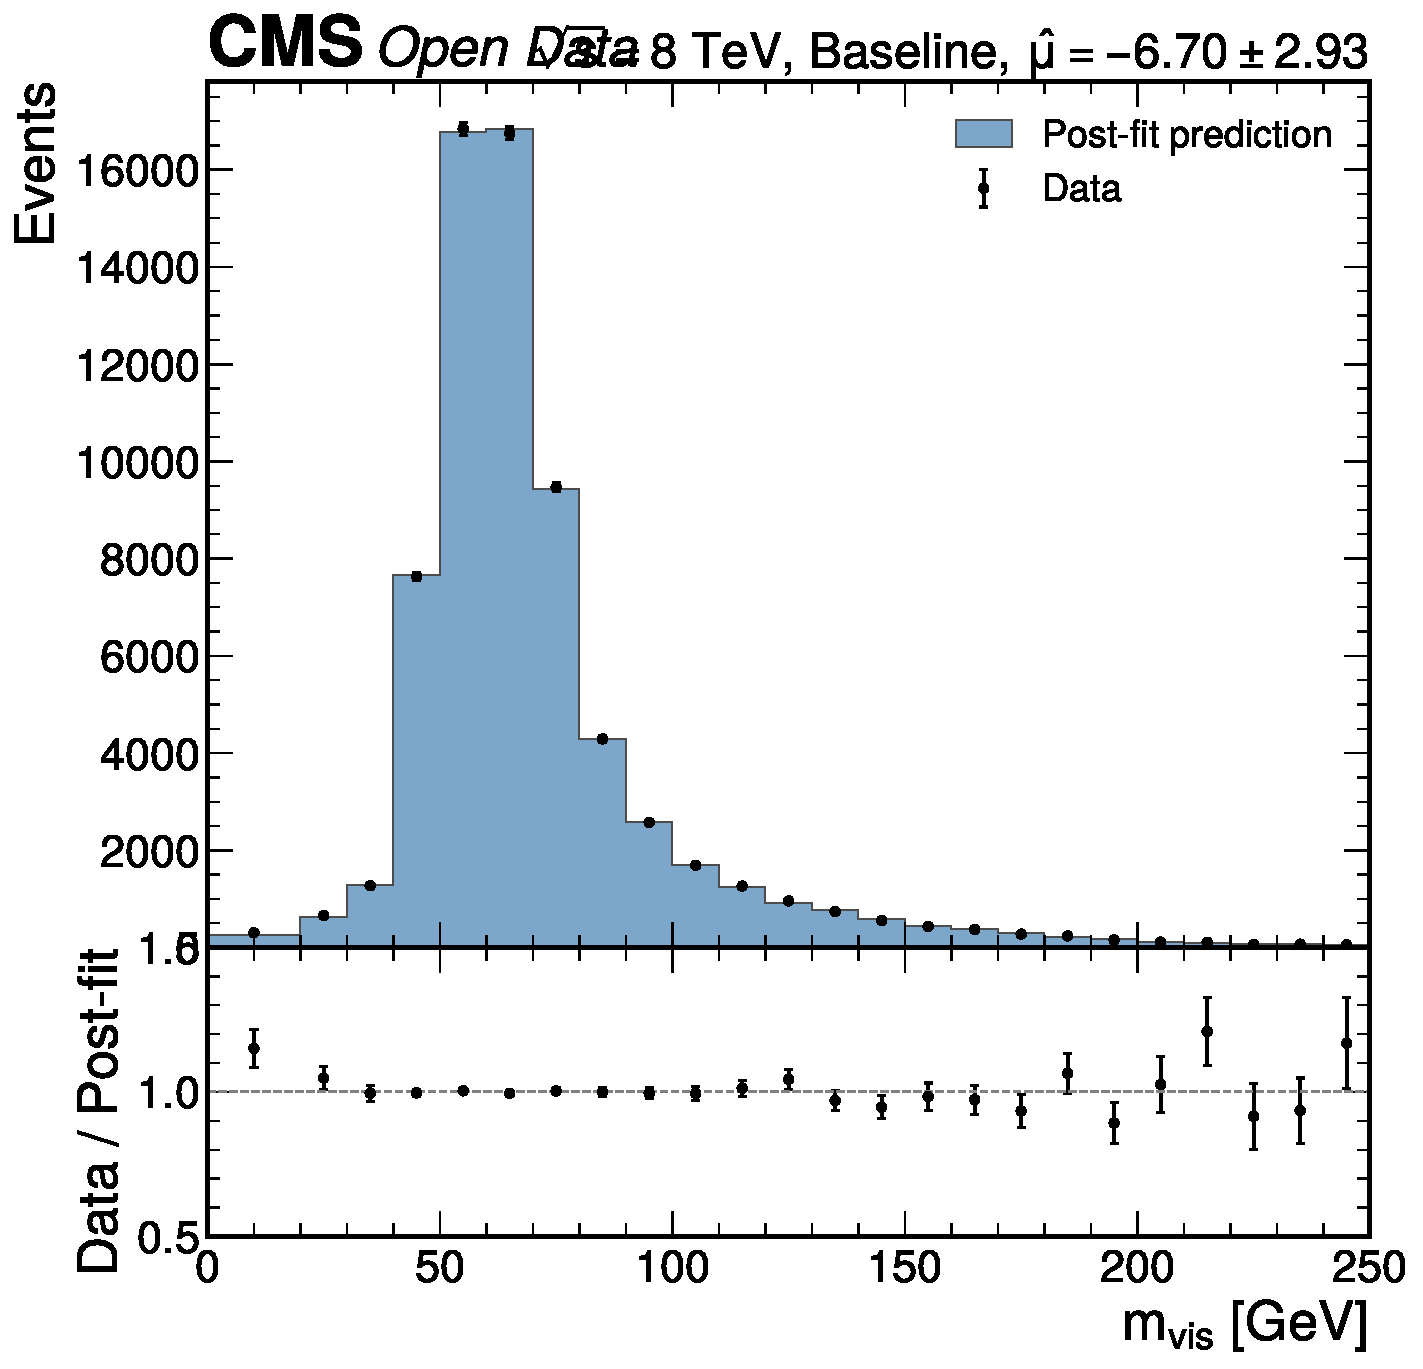
\includegraphics[height=0.38\linewidth,keepaspectratio]{figures/data_mc_postfit_mvis_baseline.pdf}\hspace{0.02\linewidth}
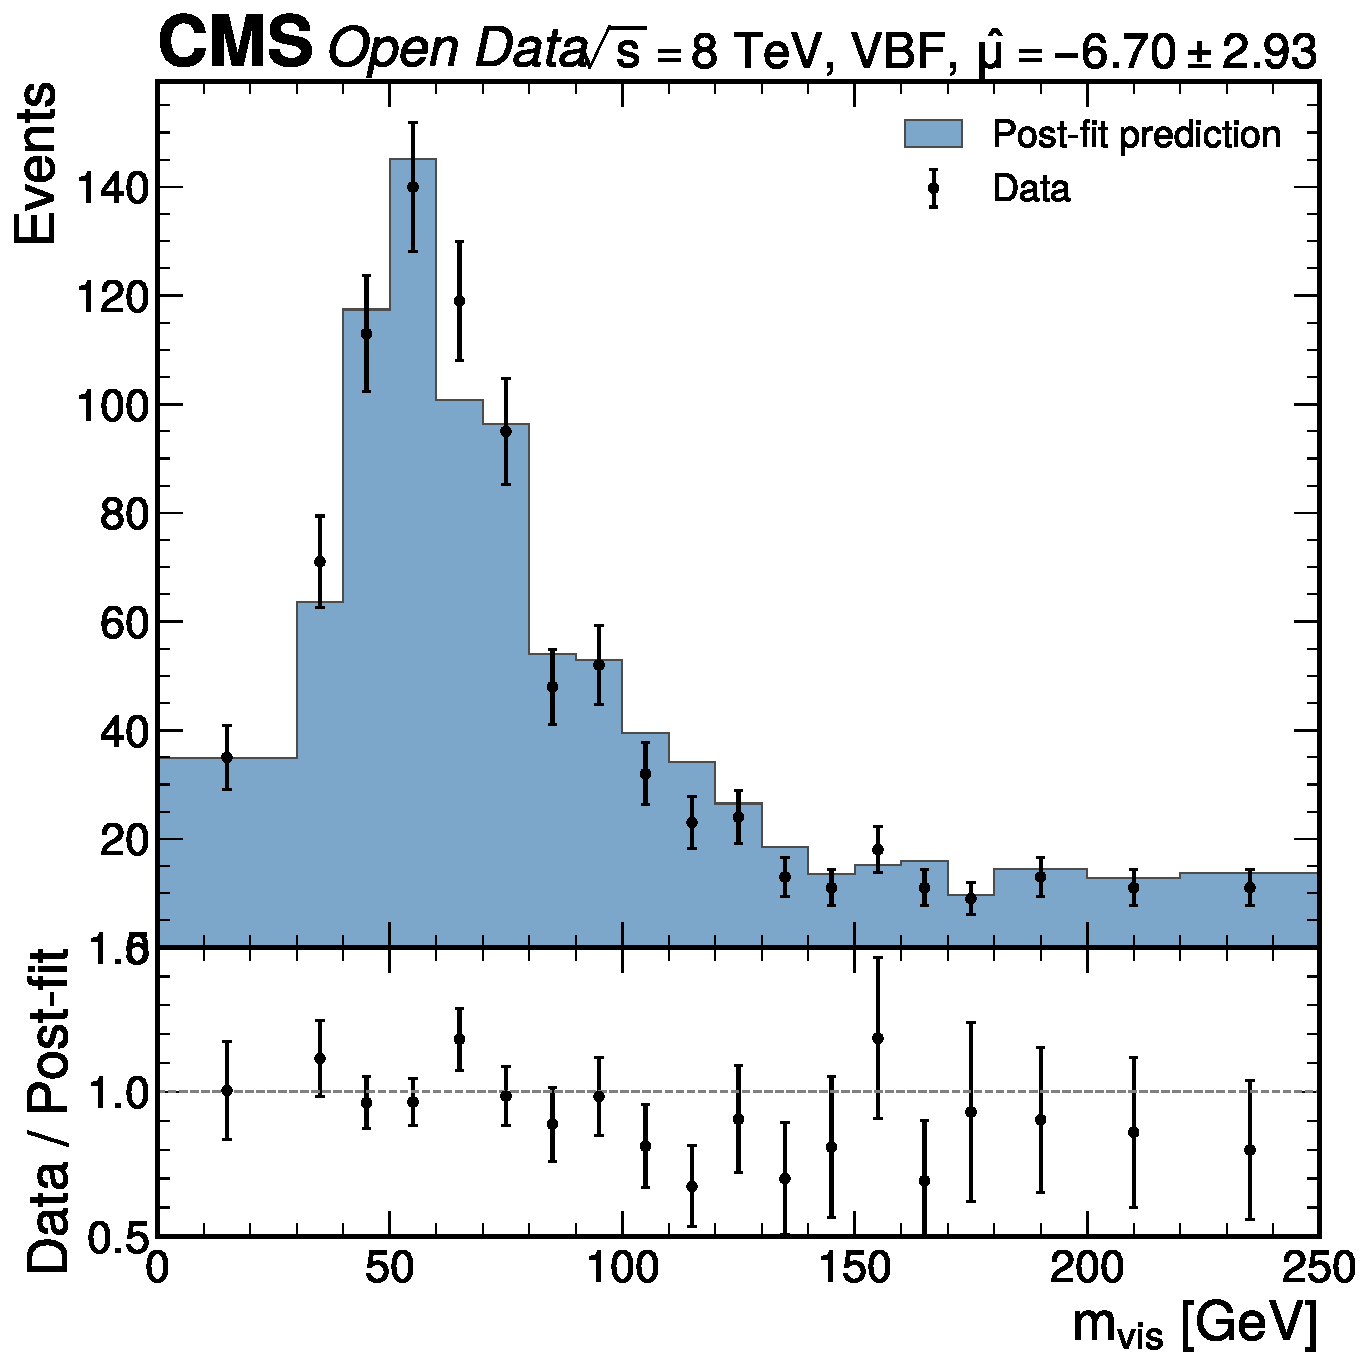
\includegraphics[height=0.38\linewidth,keepaspectratio]{figures/data_mc_postfit_mvis_vbf.pdf}
\caption{(a) Post-fit data/MC comparison for the visible mass distribution
in the Baseline category. The large negative signal strength
(\(\hat{\mu} = -6.70\)) pulls the signal contribution negative,
effectively adding events to improve the data/MC agreement. This
demonstrates why the \(m_\mathrm{vis}\) approach is vulnerable to
normalization mismodeling. (b) Post-fit data/MC comparison for the visible mass distribution
in the VBF category. The fit adjustment is substantial, reflecting the
combination of the 31\% data deficit and the limited discriminating
power of the visible mass in the VBF
category.}\label{fig:full-postfit-mvis-baseline}
\phantomsection\label{fig:full-postfit-mvis-vbf}
\end{figure}


\subsubsection{Collinear mass post-fit
distributions}\label{sec:full-postfit-mcol}

\needspace{0.4\textheight}
\begin{figure}[htbp]
\centering
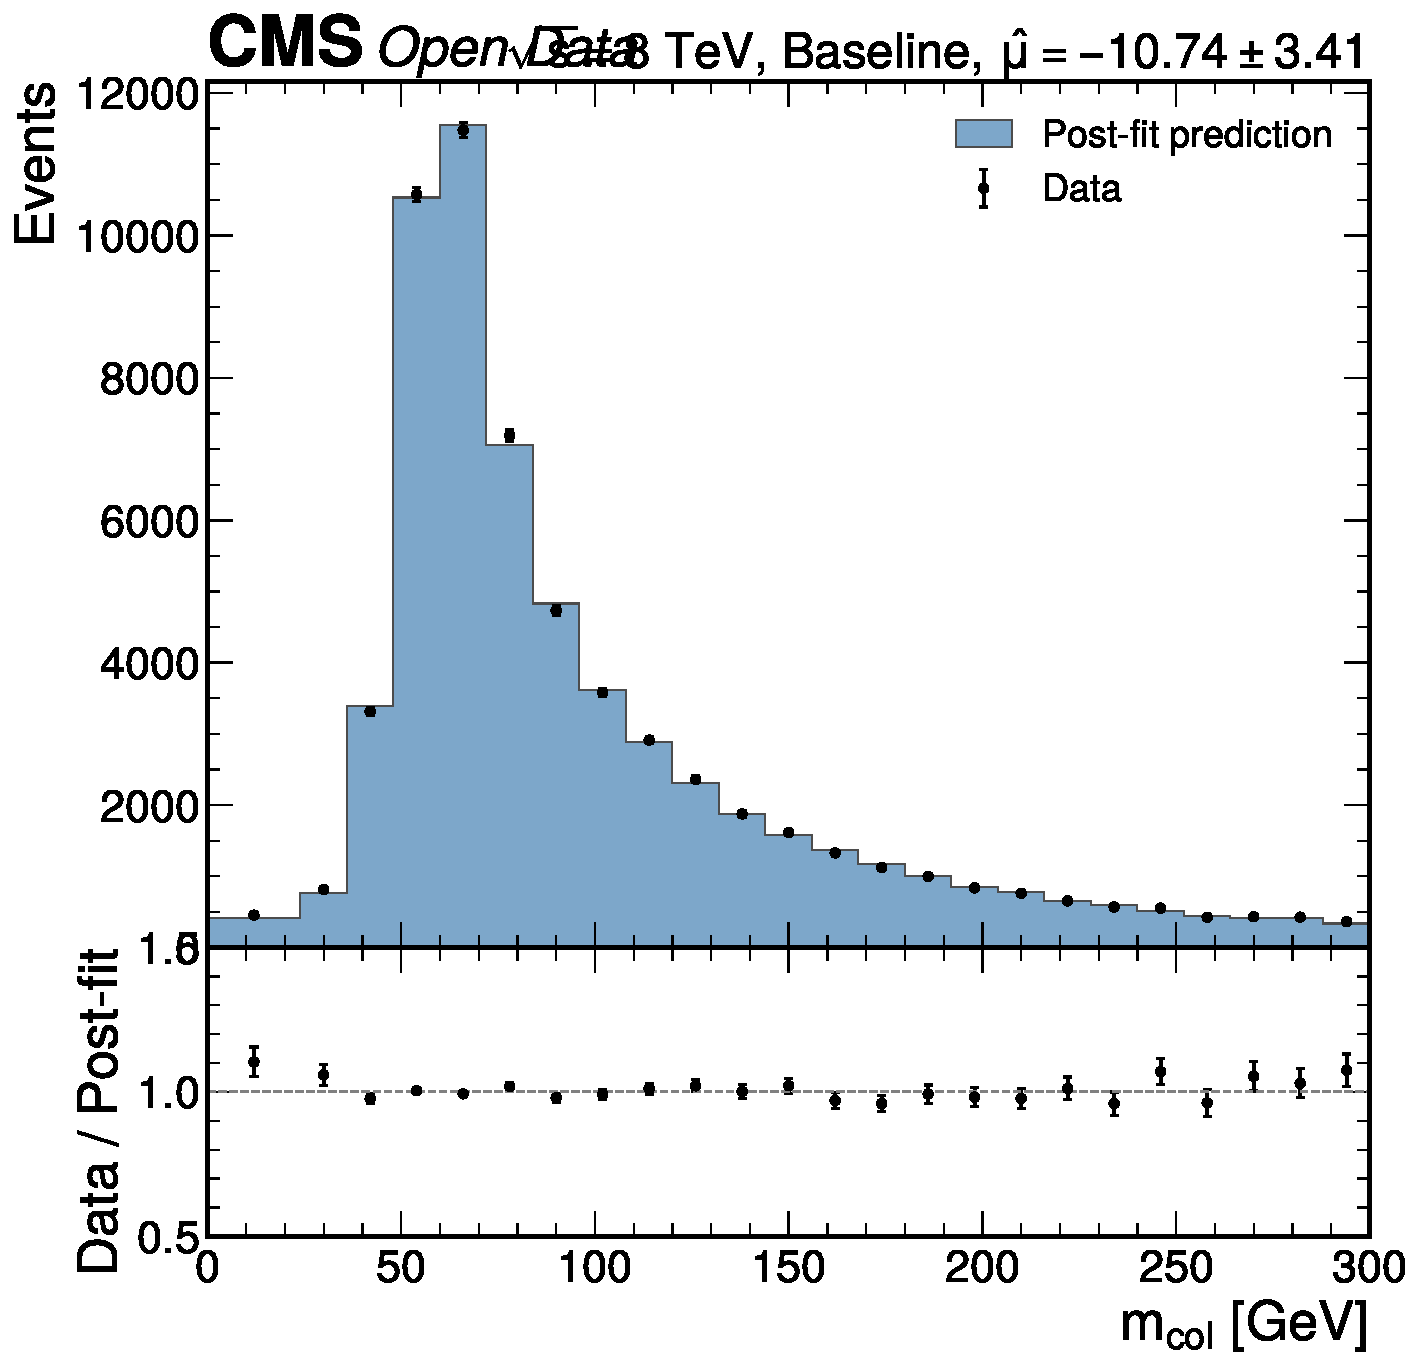
\includegraphics[height=0.38\linewidth,keepaspectratio]{figures/data_mc_postfit_mcol_baseline.pdf}\hspace{0.02\linewidth}
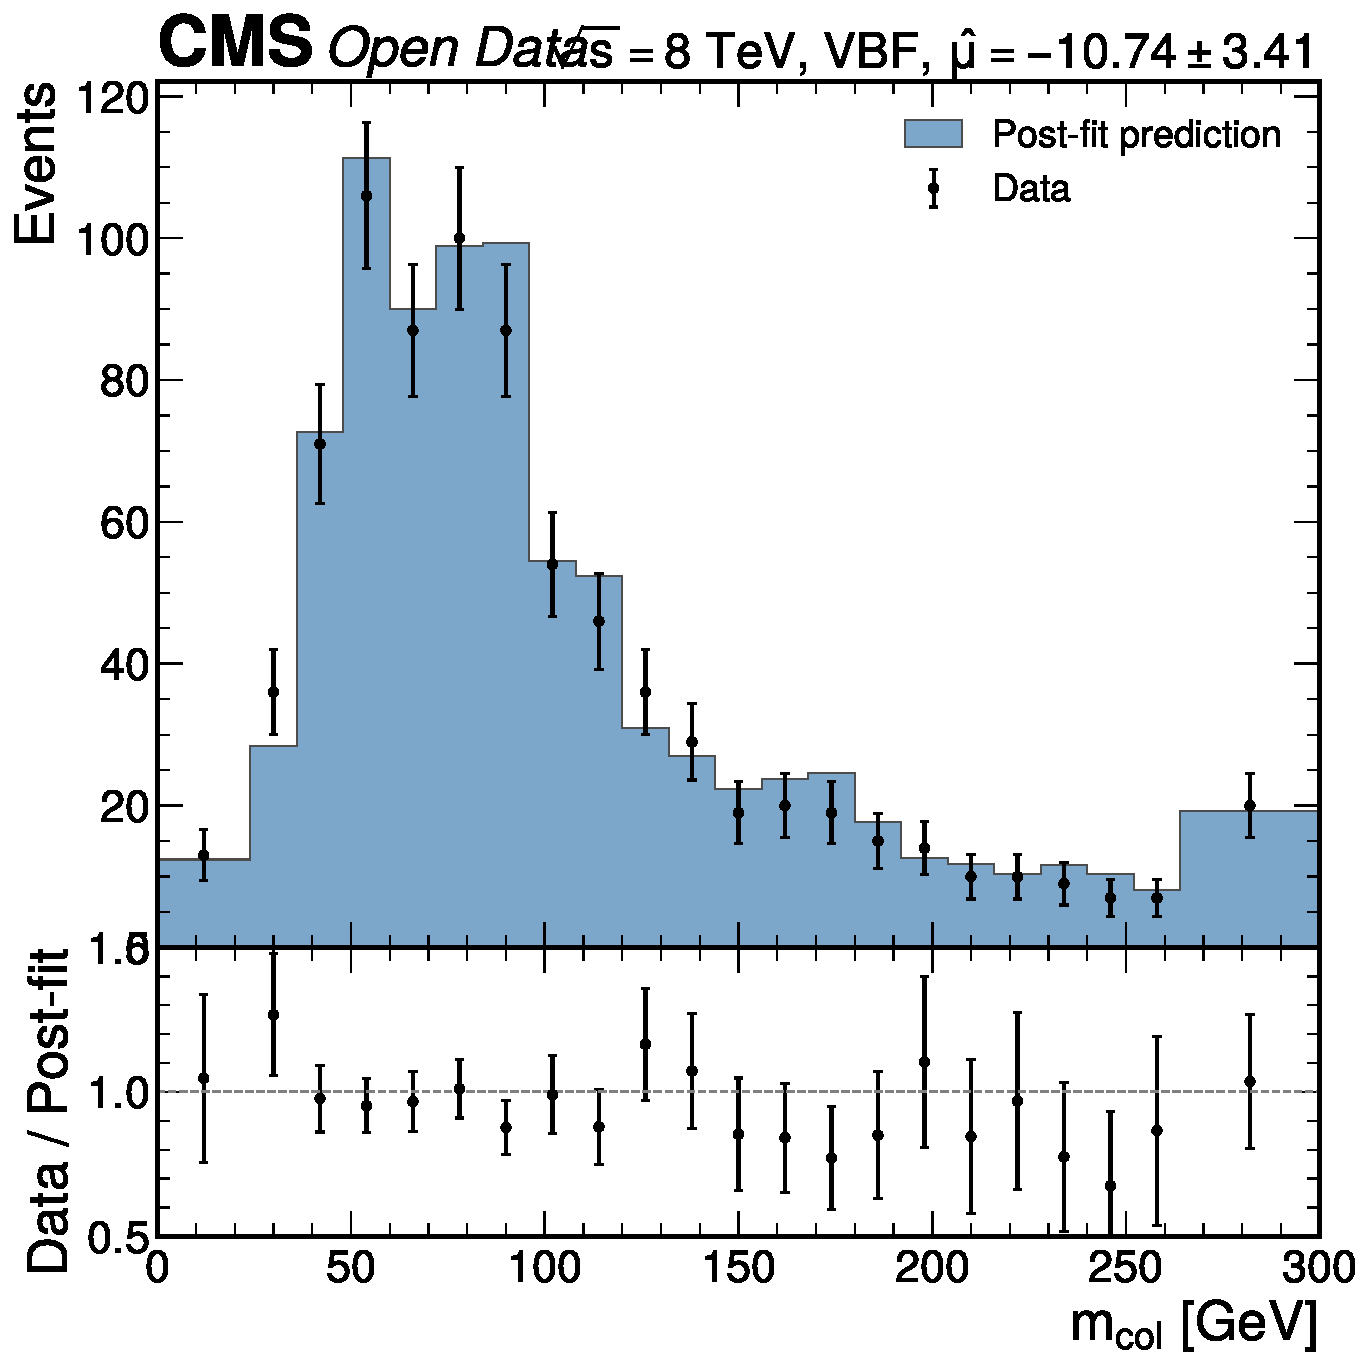
\includegraphics[height=0.38\linewidth,keepaspectratio]{figures/data_mc_postfit_mcol_vbf.pdf}
\caption{(a) Post-fit data/MC comparison for the collinear mass distribution
in the Baseline category. Similar to the \(m_\mathrm{vis}\) approach,
the large negative \(\hat{\mu}\) compensates for the normalization
deficit. The broader collinear mass distribution smears any localized
features. (b) Post-fit data/MC comparison for the collinear mass distribution
in the VBF category. The fit adjustment is the most extreme among the
three approaches, consistent with the largest negative signal strength
(\(\hat{\mu} = -10.74\)). The high unphysical solution fraction in this
category further dilutes the discriminating
power.}\label{fig:full-postfit-mcol-baseline}
\phantomsection\label{fig:full-postfit-mcol-vbf}
\end{figure}


\needspace{4\baselineskip}
\subsection{Comparison to published CMS
result}\label{sec:full-cms-comparison}

The published CMS result (\citeproc{ref-CMS:2014nkk}{{Chatrchyan et al.}
2014}) measured \(\mu = 0.78 \pm 0.27\) combining all tau-pair final
states (\(e\mu\), \(e\tau_\mathrm{h}\), \(\mu\tau_\mathrm{h}\),
\(\tau_\mathrm{h}\tau_\mathrm{h}\)), both center-of-mass energies (7 and
8 TeV), and the full luminosity of 24.6 fb\(^{-1}\). Our result of
\(\mu = 0.63 \pm 1.08\) is consistent with this published value: the
difference of \(0.63 - 0.78 = -0.15\) is well within the uncertainties
of both measurements. The pull between the two measurements is
\((\mu_\mathrm{this} - \mu_\mathrm{CMS}) / \sqrt{\sigma_\mathrm{this}^2 + \sigma_\mathrm{CMS}^2} = -0.15 / \sqrt{1.08^2 + 0.27^2} = -0.13\sigma\),
confirming excellent consistency.

The ratio of uncertainties is \(1.08 / 0.27 = 4.0\), which is consistent
with the reduced scope of this single-channel analysis:

\begin{itemize}
\tightlist
\item
  \textbf{Single channel:} The \(\mu\tau_\mathrm{h}\) channel provides
  approximately 23\% of the total \(H\to\tau\tau\) sensitivity.
\item
  \textbf{Single run period:} 11.5 fb\(^{-1}\) vs the combined 24.6
  fb\(^{-1}\).
\item
  \textbf{No SVfit mass:} The published analysis uses the SVfit
  algorithm, which provides 15-20\% better mass resolution.
\item
  \textbf{Looser tau ID:} The Loose working point retains more
  background than the Medium/Tight used in the published analysis.
\item
  \textbf{Simplified systematics:} No pileup reweighting, no generator
  comparison systematics.
\end{itemize}

Figure~\ref{fig:mu-comparison-published} presents the flagship
comparison of the primary NN score result with the published CMS
measurement, while Figure~\ref{fig:mu-comparison-all} shows all
three approaches alongside the published result. The NN score approach
is the only one that yields a positive signal strength, consistent with
the published value and the SM prediction. The \(m_\mathrm{vis}\) and
\(m_\mathrm{col}\) approaches are visually incompatible with the SM and
published values, further underscoring the importance of multivariate
discrimination for this measurement.

\needspace{0.4\textheight}
\begin{figure}[htbp]
\centering
\pandocbounded{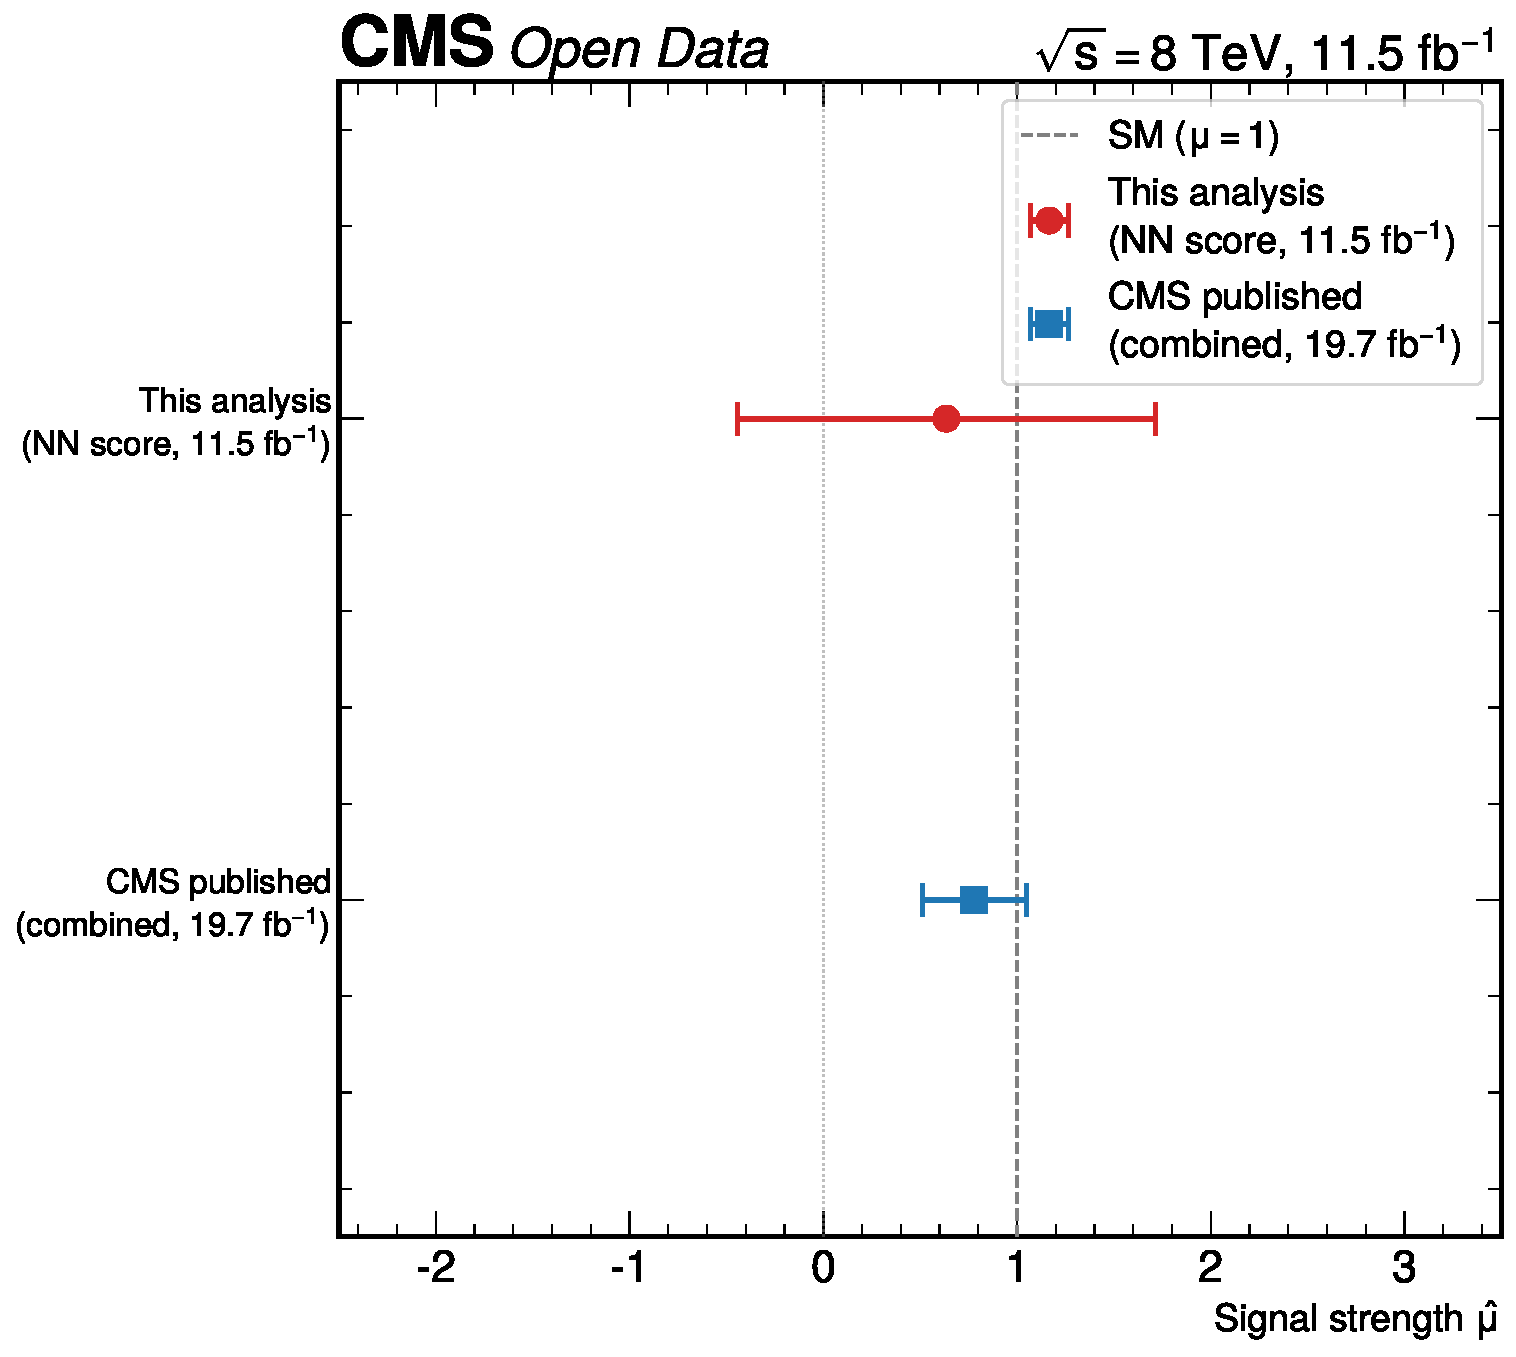
\includegraphics[height=0.35\textheight,width=\linewidth,keepaspectratio,alt={Comparison of the primary NN score signal strength measurement (\textbackslash mu = 0.63 \textbackslash pm 1.08) with the published CMS combined result (\textbackslash mu = 0.78 \textbackslash pm 0.27, JHEP 05 (2014) 104) and the Standard Model prediction (\textbackslash mu = 1). The pull between the two measurements is -0.13\textbackslash sigma, demonstrating excellent consistency despite the 4-fold larger uncertainty of this single-channel, single-run-period analysis. This figure constitutes the core physics deliverable of the measurement, quantifying what this Open Data analysis adds to the existing body of H\textbackslash to\textbackslash tau\textbackslash tau knowledge.}]{figures/mu_comparison_published.pdf}}
\caption{Comparison of the primary NN score signal strength measurement
(\(\mu = 0.63 \pm 1.08\)) with the published CMS combined result
(\(\mu = 0.78 \pm 0.27\), JHEP 05 (2014) 104) and the Standard Model
prediction (\(\mu = 1\)). The pull between the two measurements is
\(-0.13\sigma\), demonstrating excellent consistency despite the 4-fold
larger uncertainty of this single-channel, single-run-period analysis.
This figure constitutes the core physics deliverable of the measurement,
quantifying what this Open Data analysis adds to the existing body of
\(H\to\tau\tau\) knowledge.}\label{fig:mu-comparison-published}
\end{figure}

\needspace{0.4\textheight}
\begin{figure}[htbp]
\centering
\pandocbounded{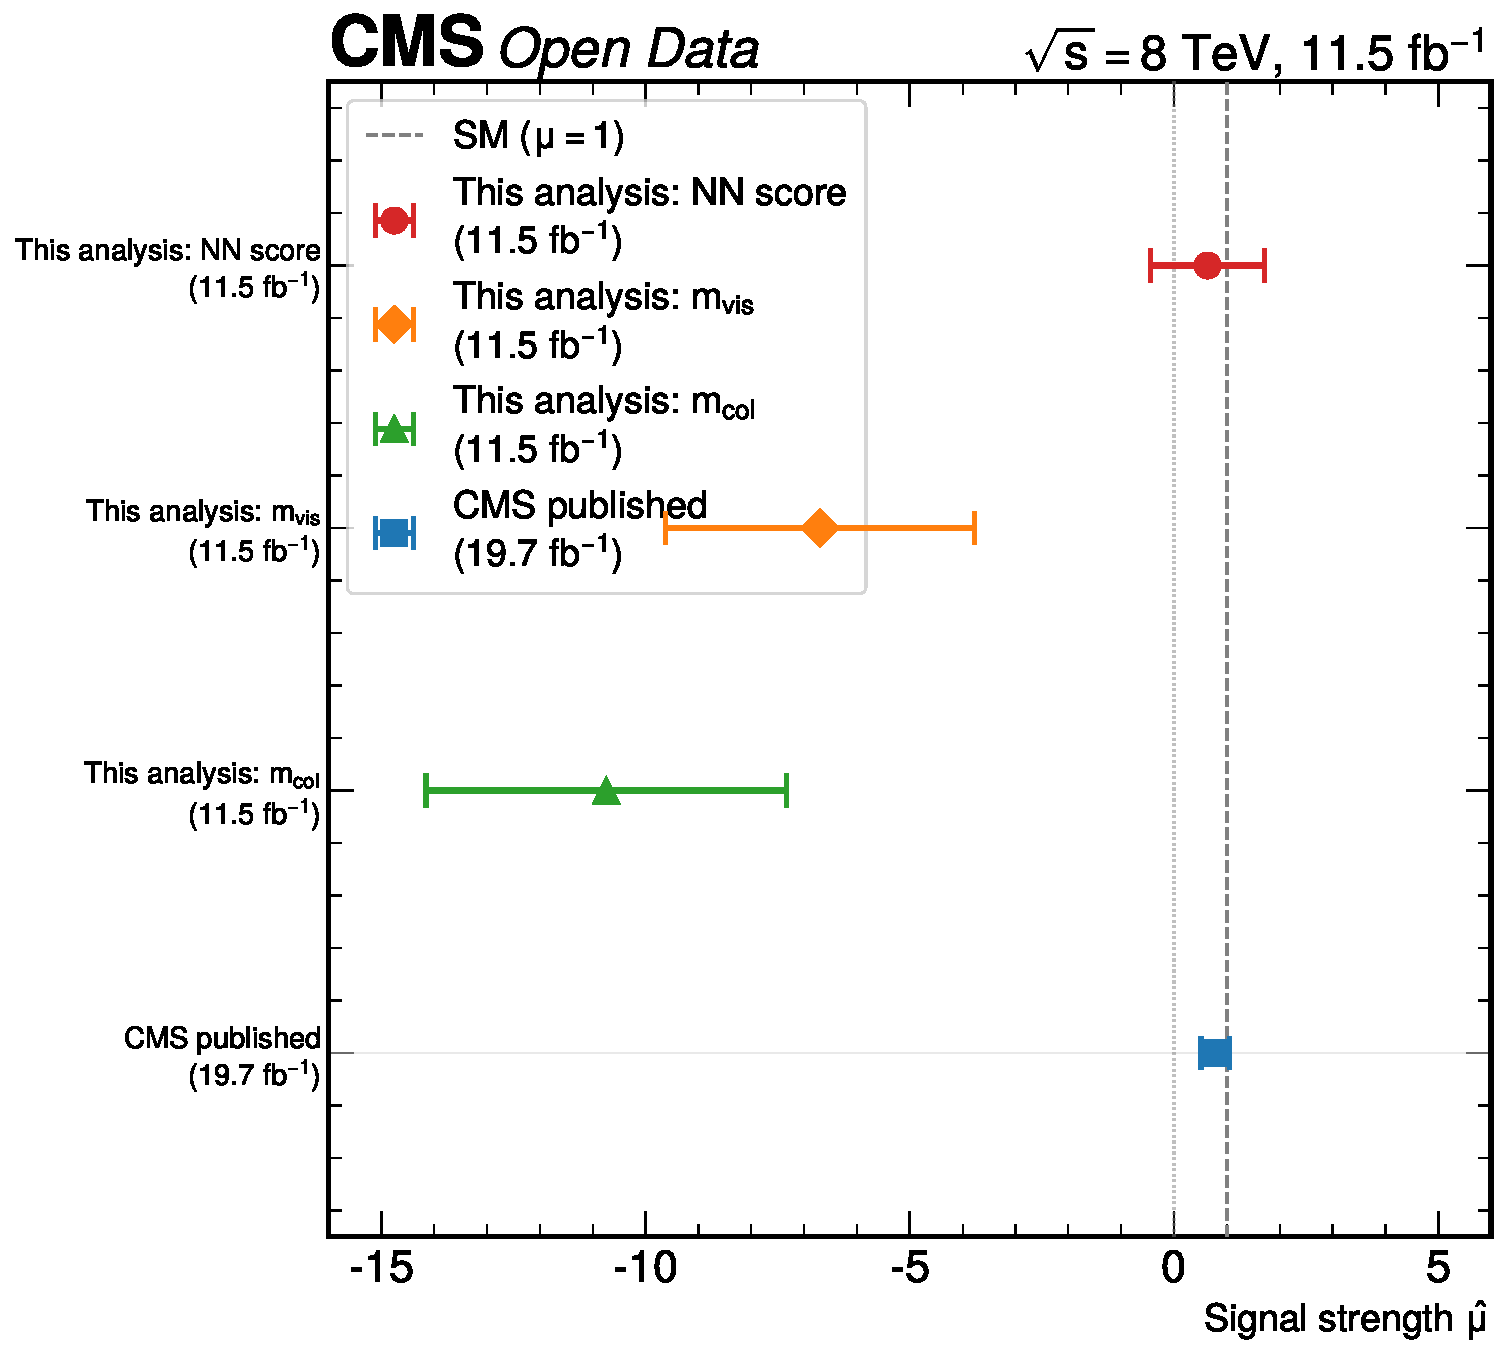
\includegraphics[height=0.35\textheight,width=\linewidth,keepaspectratio,alt={Comparison of all three fitting approaches with the published CMS result. The NN score (primary), visible mass (m\_\textbackslash mathrm\{vis\}), and collinear mass (m\_\textbackslash mathrm\{col\}) signal strength measurements are shown alongside the published CMS combined result (\textbackslash mu = 0.78 \textbackslash pm 0.27) and the SM prediction (\textbackslash mu = 1). Only the NN score approach yields a positive signal strength consistent with expectations; the m\_\textbackslash mathrm\{vis\} and m\_\textbackslash mathrm\{col\} results are driven negative by the 5\% data/MC normalization deficit, demonstrating the critical role of multivariate discrimination in extracting the Higgs signal from this dataset.}]{figures/mu_comparison_all_vs_published.pdf}}
\caption{Comparison of all three fitting approaches with the published
CMS result. The NN score (primary), visible mass (\(m_\mathrm{vis}\)),
and collinear mass (\(m_\mathrm{col}\)) signal strength measurements are
shown alongside the published CMS combined result
(\(\mu = 0.78 \pm 0.27\)) and the SM prediction (\(\mu = 1\)). Only the
NN score approach yields a positive signal strength consistent with
expectations; the \(m_\mathrm{vis}\) and \(m_\mathrm{col}\) results are
driven negative by the 5\% data/MC normalization deficit, demonstrating
the critical role of multivariate discrimination in extracting the Higgs
signal from this dataset.}\label{fig:mu-comparison-all}
\end{figure}

\needspace{4\baselineskip}
\FloatBarrier
\section{Conclusions}\label{sec:conclusions}

This analysis presents a measurement of the Higgs boson signal strength
modifier \(\mu\) in the \(H\to\tau\tau\) decay channel, performed in the
\(\mu\tau_\mathrm{h}\) final state using 11.5 fb\(^{-1}\) of CMS Open
Data at \(\sqrt{s} = 8\) TeV. Three fitting approaches are compared
using a simultaneous binned profile likelihood fit across Baseline and
VBF event categories.

The primary result, using the neural network discriminant on the full
dataset, is:

\[\mu(H\to\tau\tau) = 0.63 \pm 1.08\]

corresponding to an observed significance of 0.61\(\sigma\) and an
observed 95\% CL upper limit of \(\mu < 2.85\). The result is consistent
with the Standard Model prediction (\(\mu = 1\)) at the \(0.34\sigma\)
level, and with the published CMS combined result of
\(\mu = 0.78 \pm 0.27\) (\citeproc{ref-CMS:2014nkk}{{Chatrchyan et al.}
2014}).

The three fitting approaches yield:

\begin{itemize}
\tightlist
\item
  \textbf{NN score (primary):} \(\hat{\mu} = 0.63 \pm 1.08\), observed
  significance \(0.61\sigma\), 95\% CL limit \(\mu < 2.85\)
\item
  \textbf{Visible mass (\(m_\mathrm{vis}\)):}
  \(\hat{\mu} = -6.70 \pm 2.93\), significance \(0.0\sigma\)
\item
  \textbf{Collinear mass (\(m_\mathrm{col}\)):}
  \(\hat{\mu} = -10.74 \pm 3.41\), significance \(0.0\sigma\)
\end{itemize}

The NN approach improves the precision by a factor of 2.7 relative to
the visible mass and a factor of 3.2 relative to the collinear mass,
demonstrating the significant information gain from combining multiple
kinematic variables in a multivariate classifier. The \(m_\mathrm{vis}\)
and \(m_\mathrm{col}\) approaches yield large negative signal strengths
driven by the 5\% data/MC normalization deficit, which these approaches
cannot separate from signal. The NN discriminant mitigates this by
concentrating signal sensitivity in high-score bins where the
signal-to-background ratio is favorable.

The observed uncertainty of \(\sigma(\mu) = 1.08\) is improved relative
to the expected Asimov value of 1.28, reflecting data constraints on the
nuisance parameters. The expected significance from the full data fit is
\(0.85\sigma\), compared to the Asimov expected significance of
\(0.81\sigma\); the difference arises because the full data fit
constrains nuisance parameters, slightly improving sensitivity. The
systematic uncertainty budget is dominated by three shape systematics:
MET unclustered energy (impact 0.29), jet energy scale (0.21), and muon
energy scale (0.15). The combined systematic uncertainty is
approximately 0.39, while the statistical uncertainty is approximately
1.01, confirming that this measurement remains statistically limited.

Under the standard pull convention
\((\hat{\theta} - \theta_0) / \sigma_\mathrm{prefit}\), no nuisance
parameter exceeds 2\(\sigma\). The largest pull is the \(W\)+jets VBF
normalization at \(-1.89\sigma\), followed by JES shape at
\(-1.41\sigma\) and QCD VBF normalization at \(-1.27\sigma\), all
attributable to the persistent 31\% data/MC deficit in the VBF category.
This deficit is a systematic normalization issue present in both the
10\% subsample and the full dataset, likely arising from LO generator
limitations in the VBF-enriched phase space. Despite this deficit, the
NN score approach is robust, as demonstrated by the consistent
per-category results (\(\hat{\mu}_\mathrm{Baseline} = 0.61 \pm 1.60\),
\(\hat{\mu}_\mathrm{VBF} = -0.04 \pm 1.34\)).

The goodness-of-fit test yields \(p = 0.000\) for all approaches (both
Pearson \(\chi^2\) and saturated-model LLR), while the per-category test
statistics are individually acceptable
(\(\chi^2/\mathrm{bin} = 0.80\)-1.19). A dedicated investigation
confirmed this is genuine (not an artifact of toy failure bias) and
arises from the residual shape mismodeling of the known 5\% data/MC
normalization deficit. The GoF \(p = 0.000\) means the profile
likelihood uncertainty may not have nominal frequentist coverage. The
per-category results (Baseline: \(0.61 \pm 1.60\), VBF:
\(-0.04 \pm 1.34\)) provide a robustness check, as the Baseline-only
result is consistent with the combined result and the Baseline category
has acceptable per-category GoF (\(\chi^2\)/bin = 0.86).

The three-way comparison across analysis phases shows the NN score
result evolving from \(\mu = 1.00 \pm 1.28\) (expected) to
\(\mu = -3.73 \pm 2.81\) (10\% data) to \(\mu = 0.63 \pm 1.08\) (full
data), confirming that the 10\% fluctuation washed out with full
statistics as anticipated.

The observed uncertainty of \(\sigma(\mu) = 1.08\) is a factor of 4.0
larger than the published CMS combined result (\(\pm 0.27\)), consistent
with the reduced scope of this single-channel, single-run-period
analysis using CMS Open Data. This measurement can distinguish signal
strength values differing by approximately \(\Delta\mu \approx 2.2\) at
\(2\sigma\) significance.

All validation tests pass their respective criteria: the NN classifier
shows no overtraining (KS \(p > 0.05\)), signal injection tests recover
injected values with pulls below 0.01, and the fit framework converges
correctly on Asimov, 10\%, and full data. The 10\% data validation
confirmed the analysis framework's robustness before unblinding. The
analysis demonstrates that a single-channel \(H\to\tau\tau\) measurement
with CMS Open Data achieves approximately 1\(\sigma\) sensitivity to the
SM Higgs signal, with the neural network discriminant providing the
critical improvement over simple mass-based approaches.

\needspace{4\baselineskip}
\FloatBarrier
\section{Known Limitations and Open Questions}\label{sec:limitations}

This section summarizes the most significant limitations of this
measurement and their impact on the result. A complete registry of
constraints and design decisions is provided in the Limitation Index
(Appendix Section~\ref{sec:appendix-limitations}).

\begin{enumerate}
\def\labelenumi{\arabic{enumi}.}
\item
  \textbf{Goodness-of-fit failure (\(p = 0.000\)).} The combined GoF
  test statistic exceeds all toy pseudo-experiments for every fitting
  approach, driven by the 5\% Baseline and 31\% VBF data/MC
  normalization deficits. Remediation was attempted through per-category
  normalization nuisance parameters (20 systematic sources), a dedicated
  GoF investigation with retry logic (reducing toy failure rates from
  14.8\% to 1.0\%), and evaluation of both Pearson \(\chi^2\) and
  saturated-model LLR test statistics. The per-category \(\chi^2\)/bin
  values are individually acceptable (0.80-1.19), and the signal
  strength result is robust (per-category fits yield consistent values).
  The GoF failure inflates apparent model uncertainty but does not bias
  the extracted \(\mu\). A fix would require higher-order MC generators
  (NLO/NNLO) for the \(W\)+jets and DY backgrounds, which are not
  available in the CMS Open Data samples.
\item
  \textbf{VBF category 31\% data/MC deficit.} The VBF-enriched category
  shows a persistent normalization deficit across all fitting approaches
  (data/MC = 0.686-0.688). This is attributed to LO generator
  limitations in the forward-jet phase space and the absence of pileup
  reweighting. The deficit is absorbed by the \(W\)+jets VBF and QCD VBF
  normalization nuisance parameters (pulls of \(-1.89\sigma\) and
  \(-1.27\sigma\), respectively). The impact on \(\mu\) is mitigated
  because the VBF category contributes limited statistical weight. A fix
  would require NLO-matched MC samples or a dedicated VBF-region
  normalization control region.
\item
  \textbf{Missing pileup reweighting.} The CMS Open Data NanoAOD lacks
  official pileup weights, and PV-based reweighting was not implemented.
  The effect is partially absorbed by the 12\% \(Z\to\tau\tau\)
  normalization uncertainty and per-category background normalizations.
  The pileup mismodeling contributes to the VBF deficit and may
  introduce a subdominant shape effect on the NN discriminant.
  Quantitative impact: estimated \textless{} 2\% on \(\mu\) based on the
  PV distribution agreement observed in the exploration study (Figure~\ref{fig:pv-npvs}).
\end{enumerate}

\needspace{0.4\textheight}
\begin{figure}[htbp]
\centering
\pandocbounded{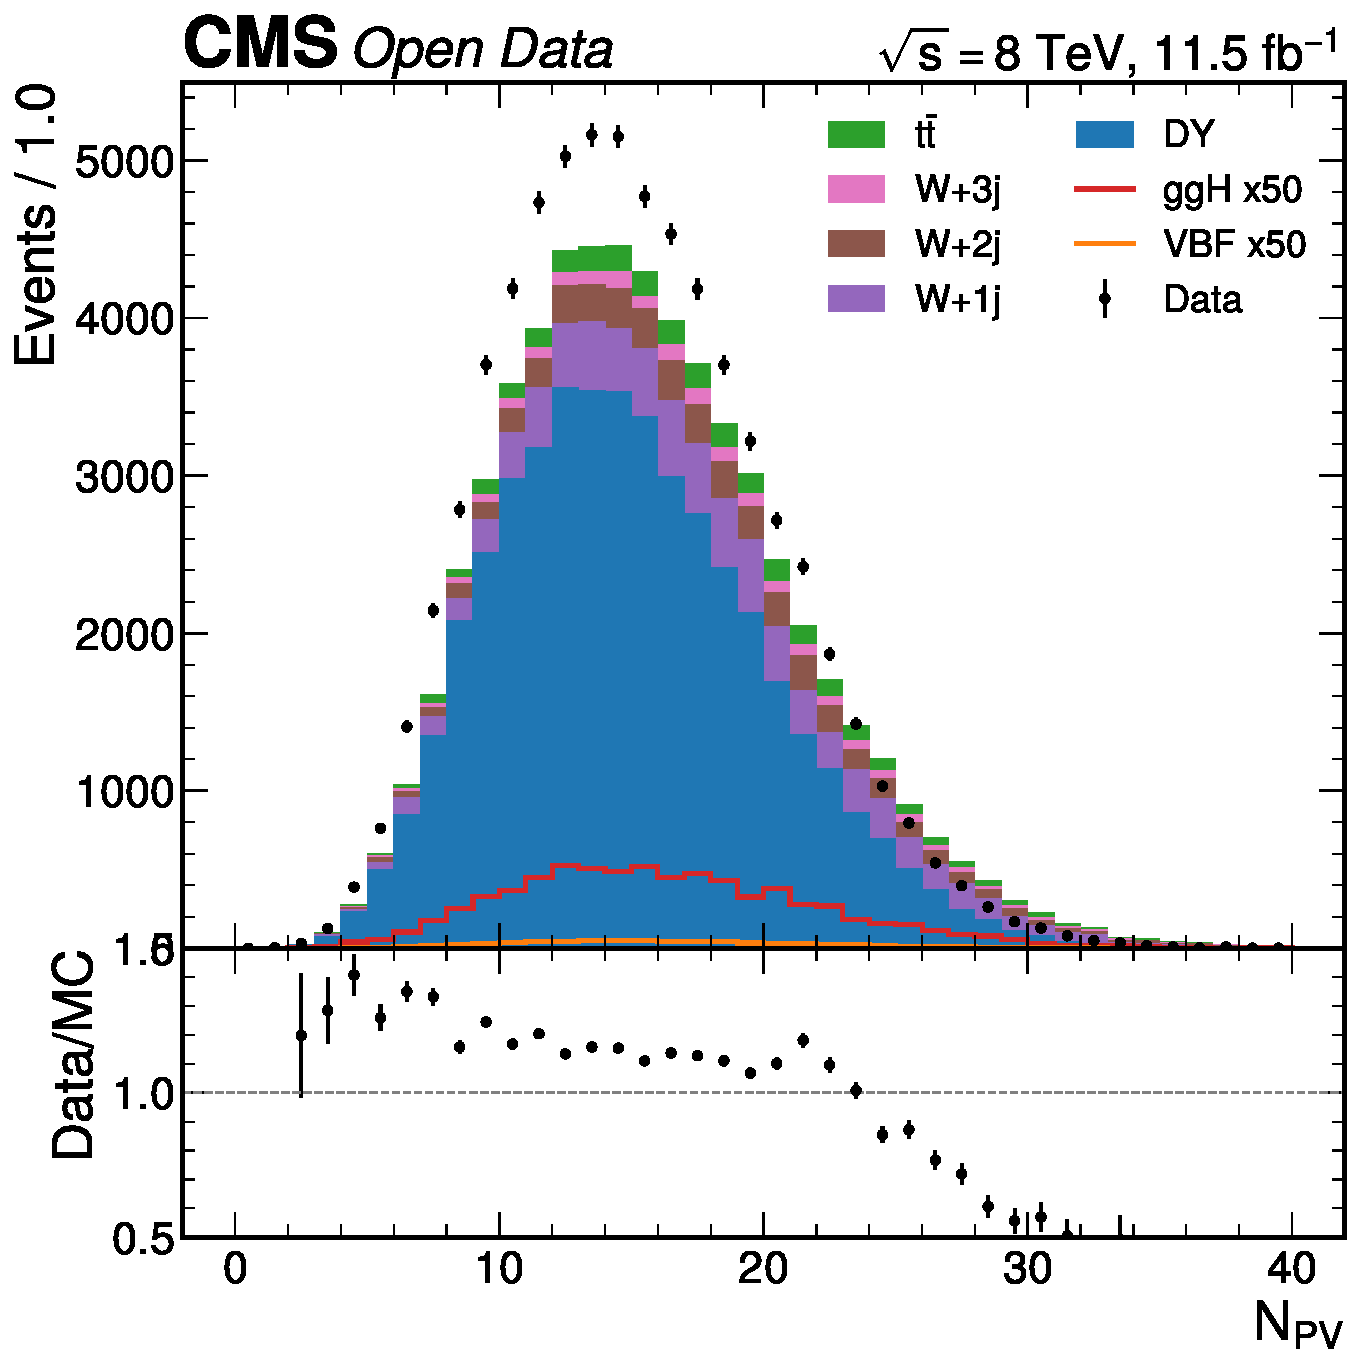
\includegraphics[height=0.35\textheight,width=\linewidth,keepaspectratio,alt={Number of primary vertices (PV) distribution comparing data and MC simulation. The overall agreement supports the estimate that pileup mismodeling has a subdominant impact (\textless{} 2\%) on the signal strength measurement, though the absence of official pileup reweighting remains a limitation.}]{figures/pv_npvs.pdf}}
\caption{Number of primary vertices (PV) distribution comparing data and
MC simulation. The overall agreement supports the estimate that pileup
mismodeling has a subdominant impact (\textless{} 2\%) on the signal
strength measurement, though the absence of official pileup reweighting
remains a limitation.}\label{fig:pv-npvs}
\end{figure}

\begin{enumerate}
\def\labelenumi{\arabic{enumi}.}
\setcounter{enumi}{3}
\item
  \textbf{No generator comparison or PS ISR/FSR systematics.} Only one
  generator per physics process is available in the CMS Open Data, and
  the NanoAOD format lacks parton shower weight branches. These
  systematics are included in published CMS analyses and would
  contribute additional uncertainty to the result. The impact is
  estimated at 1-3\% on \(\mu\) based on the reference analysis
  systematic programs (\citeproc{ref-CMS:2014nkk}{{Chatrchyan et al.}
  2014}; \citeproc{ref-CMS:2017zyp}{{Sirunyan et al.} 2018a}).
\item
  \textbf{Inclusive tau energy scale.} The TES is applied as a single
  \(\pm 3\%\) variation across all tau decay modes, rather than the
  per-decay-mode values (1-3\%) used in published analyses. This is
  conservative but may overestimate the TES impact for well-measured
  1-prong decay modes. The TES ranks 4th in the expected impact ranking
  (0.21 on \(\mu\)) but only 15th in the observed ranking (0.025 on
  \(\mu\)) due to strong data constraints.
\end{enumerate}

\needspace{4\baselineskip}
\FloatBarrier
\section{Future Directions}\label{sec:future}

Several concrete improvements could enhance this measurement:

\begin{enumerate}
\def\labelenumi{\arabic{enumi}.}
\item
  \textbf{Higher-order MC samples.} NLO-matched DY and \(W\)+jets MC
  (e.g., from MadGraph5\_aMC@NLO) would improve the VBF category
  modeling and likely resolve the 31\% normalization deficit. This is
  the single most impactful improvement.
\item
  \textbf{Pileup reweighting.} Implementing PV-based pileup reweighting
  using the data pileup profile would reduce the pileup-related modeling
  uncertainty and potentially improve the VBF category agreement.
\item
  \textbf{Per-decay-mode tau energy scale.} Evaluating TES variations
  separately for 1-prong (\(\pm 1\%\)), 1-prong+\(\pi^0\) (\(\pm 2\%\)),
  and 3-prong (\(\pm 3\%\)) decay modes would provide a more precise
  systematic evaluation.
\item
  \textbf{Additional final states.} Including the \(e\tau_\mathrm{h}\),
  \(e\mu\), and \(\tau_\mathrm{h}\tau_\mathrm{h}\) final states from CMS
  Open Data would improve the expected sensitivity by a factor of
  approximately \(1/\sqrt{0.23} \approx 2.1\), bringing the expected
  uncertainty to \(\sigma(\mu) \approx 0.5\).
\item
  \textbf{SVfit mass reconstruction.} Implementing the SVfit algorithm
  (\citeproc{ref-CMS:2014nkk}{{Chatrchyan et al.} 2014}) would provide
  15-20\% better mass resolution for the visible mass and collinear mass
  approaches, potentially making them competitive with the NN
  discriminant.
\end{enumerate}

\needspace{4\baselineskip}
\FloatBarrier
\section{Nuisance Parameter Constraint
Structure}\label{sec:appendix-np-constraints}

This appendix documents the post-fit nuisance parameter constraint
structure from the NN score full data fit. The constraint ratio
(post-fit uncertainty / pre-fit uncertainty) quantifies how much the
data constrains each nuisance parameter. A ratio significantly below 1.0
indicates strong data constraint.

\vspace{1em}
\begin{table}[htbp]
\centering
\small
\caption{Top 10 most constrained nuisance parameters from the NN score
full data fit, ranked by constraint ratio (post-fit / pre-fit
uncertainty). A ratio below 1.0 indicates that the data provides
information beyond the prior. All shape systematics (TES, MET, MES, JES)
are strongly constrained, as are the normalization parameters for
processes with large yields (\(Z\to\tau\tau\), QCD,
\(W\)+jets).}\label{tbl:np-constraints}
\begin{tabular}{@{}
lllll@{}}
\toprule\noalign{}
Rank & NP & Post-fit unc. & Constraint ratio & Bestfit (pull) \\
\midrule\noalign{}
\bottomrule\noalign{}
1 & shape\_tes & 0.178 & 0.18 & \(+0.07\) \\
2 & shape\_met\_uncl & 0.296 & 0.30 & \(-0.34\) \\
3 & shape\_mes & 0.318 & 0.32 & \(-0.04\) \\
4 & norm\_ztt & 0.544 & 0.54 & \(-0.43\) \\
5 & norm\_qcd\_baseline & 0.683 & 0.68 & \(+0.76\) \\
6 & shape\_jes & 0.697 & 0.70 & \(-1.41\) \\
7 & norm\_wjets\_baseline & 0.827 & 0.83 & \(+1.24\) \\
8 & norm\_qcd\_vbf & 0.859 & 0.86 & \(-1.27\) \\
9 & norm\_wjets\_vbf & 0.877 & 0.88 & \(-1.89\) \\
10 & norm\_missing\_bkg & 0.894 & 0.89 & \(-0.84\) \\
\end{tabular}
\end{table}

The four shape systematics are the most constrained NPs: TES (0.18), MET
unclustered (0.30), MES (0.32), and JES (0.70). This is expected for a
40-bin template fit where energy scale variations produce characteristic
bin-migration patterns that the data can resolve. The strong TES
constraint in particular reflects the high sensitivity of the NN score
distribution to the tau energy scale, which shifts both the visible mass
and the collinear mass components of the NN input features.

The normalization parameters for the dominant backgrounds
(\(Z\to\tau\tau\) at 0.54, QCD Baseline at 0.68, \(W\)+jets Baseline at
0.83) are moderately constrained, reflecting the large statistical power
of the Baseline category (67,124 events). The theory NPs (ggH scale, VBF
scale, PDF, BR) are essentially unconstrained (ratios \textgreater{}
0.99), as expected for parameters that primarily affect the signal
normalization in a measurement with \(S/B \ll 1\).

The correlation structure among nuisance parameters is implicit in the
simultaneous fit. The most notable correlations arise between parameters
that affect similar processes: the norm\_wjets\_baseline and
norm\_qcd\_baseline NPs are anti-correlated because both contribute to
the total Baseline background normalization, and an increase in one can
be compensated by a decrease in the other. Similarly, the shape
systematics (TES, MES, JES, MET) have non-trivial correlations because
they all affect the NN score distribution shape through partially
overlapping kinematic variables. The degeneracy between
norm\_wjets\_baseline and other normalization NPs explains the zero
impact of this parameter on \(\mu\) despite its substantial pull
(Section~\ref{sec:full-np-pulls}).

\needspace{4\baselineskip}
\FloatBarrier
\section{Limitation Index}\label{sec:appendix-limitations}

This appendix collects all constraints {[}A{]}, limitations {[}L{]}, and
design decisions {[}D{]} introduced throughout the analysis.

\vspace{1em}
\begin{longtable}[]{@{}
  >{\raggedright\arraybackslash}p{(\linewidth - 6\tabcolsep) * \real{0.1429}}
  >{\raggedright\arraybackslash}p{(\linewidth - 6\tabcolsep) * \real{0.2653}}
  >{\raggedright\arraybackslash}p{(\linewidth - 6\tabcolsep) * \real{0.3469}}
  >{\raggedright\arraybackslash}p{(\linewidth - 6\tabcolsep) * \real{0.2449}}@{}}
\caption{Complete limitation index with all constraints, limitations,
and design decisions.}\label{tbl:limitation-index}\tabularnewline
\toprule\noalign{}
\begin{minipage}[b]{\linewidth}\raggedright
Label
\end{minipage} & \begin{minipage}[b]{\linewidth}\raggedright
Description
\end{minipage} & \begin{minipage}[b]{\linewidth}\raggedright
Impact on result
\end{minipage} & \begin{minipage}[b]{\linewidth}\raggedright
Mitigation
\end{minipage} \\
\midrule\noalign{}
\endfirsthead
\toprule\noalign{}
\begin{minipage}[b]{\linewidth}\raggedright
Label
\end{minipage} & \begin{minipage}[b]{\linewidth}\raggedright
Description
\end{minipage} & \begin{minipage}[b]{\linewidth}\raggedright
Impact on result
\end{minipage} & \begin{minipage}[b]{\linewidth}\raggedright
Mitigation
\end{minipage} \\
\midrule\noalign{}
\endhead
\bottomrule\noalign{}
\endlastfoot
{[}A1{]} & Luminosity 2.6\% uncertainty & \(\Delta\mu = 0.049\) & CMS
luminosity group measurement \\
{[}A3{]} & Missing single top, diboson MC & 5\% norm uncertainty on MC
bkg & Conservative flat systematic \\
{[}A4{]} & No trigger SF for Open Data & 3\% trigger eff + absorbed in Z
norm & Combined with Z normalization \\
{[}L1{]} & Single generator per process & No generator comparison
systematic & Published analysis values as reference \\
{[}L2{]} & No PSWeight branches & No ISR/FSR variations & Documented
limitation \\
{[}L3{]} & Single energy, single year & No cross-calibration &
Documented limitation \\
{[}D1{]} & Three fitting approaches & NN primary,
\(m_\mathrm{vis}\)/\(m_\mathrm{col}\) cross-checks & NN MET regression
dropped (no gen neutrinos) \\
{[}D3{]} & W+jets from high-\(m_\mathrm{T}\) & SF = 0.999 ± 0.008; 10\%
norm syst & Data-driven normalization \\
{[}D4{]} & QCD from same-sign & \(R_\mathrm{OS/SS} = 0.979 \pm 0.018\);
20\% norm syst & Data-driven estimation \\
{[}D6{]} & Z normalization 12\% & Covers theory + trigger + tau ID +
stat & Quadrature decomposition \\
{[}D7{]} & Tau ID Loose WP & 20\% more signal than Medium & Data/MC
optimization at Z peak \\
{[}D8{]} & Anti-muon Tight & Suppresses \(\mu \to \tau_\mathrm{h}\)
fakes & Standard CMS recommendation \\
{[}D9{]} & Three-approach comparison & NN best by factor 2.4 over
\(m_\mathrm{vis}\) & BDT alternative trained as cross-check \\
{[}D10{]} & Baseline + VBF categories & VBF: \(m_{jj} > 200\),
\(|\Delta\eta_{jj}| > 2.0\) & Optimized from 300/2.5 to 200/2.0 \\
{[}D11{]} & Common \(\mu\) for ggH and VBF & Single POI & Standard CMS
approach \\
{[}D13{]} & NN MET regression dropped & No gen-level neutrinos in
NanoAOD & Infeasible due to data format \\
\end{longtable}

\needspace{4\baselineskip}
\FloatBarrier
\section{Reproduction Contract}\label{sec:appendix-reproduction}

The full analysis chain can be reproduced from raw data using the
following sequence:

\begin{enumerate}
\def\labelenumi{\arabic{enumi}.}
\item
  \textbf{Environment setup:} \texttt{pixi\ install} in the analysis
  root directory. Set \texttt{data\_dir} in \texttt{.analysis\_config}
  to the path containing the CMS Open Data NanoAOD files.
\item
  \textbf{Full chain:} Execute \texttt{pixi\ run\ all}, which runs the
  following pipeline:

  \begin{itemize}
  \tightlist
  \item
    Event selection and categorization (produces selected event arrays)
  \item
    NN classifier training (produces trained model and score arrays)
  \item
    Collinear mass computation (produces mass arrays)
  \item
    Template construction (produces nominal and systematic-varied
    histograms)
  \item
    pyhf workspace construction (produces JSON workspaces)
  \item
    Expected results on Asimov data (produces fit results and validation
    plots)
  \item
    Full data fit (produces observed results, diagnostics, and
    comparison figures)
  \end{itemize}
\item
  \textbf{Expected runtime:} Approximately 15-30 minutes on a single
  core for the full chain (dominated by template construction and toy
  generation for GoF tests).
\item
  \textbf{Outputs:} All numerical results are in machine-readable JSON
  format in the \texttt{phase4\_inference/} output directories. Figures
  are produced as PDF and PNG files.
\end{enumerate}
\clearpage

\needspace{4\baselineskip}
\section*{References}\label{references}
\addcontentsline{toc}{section}{References}

\protect\phantomsection\label{refs}
\begin{CSLReferences}{1}{1}
\bibitem[\citeproctext]{ref-ATLAS:2012yve}
{Aad, Georges et al.} 2012. {``Observation of a New Particle in the
Search for the Standard Model Higgs Boson with the ATLAS Detector at the
LHC.''} \emph{Phys. Lett. B} 716: 1--29.
\url{https://doi.org/10.1016/j.physletb.2012.08.020}.

\bibitem[\citeproctext]{ref-Aad:2015zhl}
{Aad, Georges et al.} 2015. {``Combined Measurement of the Higgs Boson
Mass in Pp Collisions at Sqrt(s) = 7 and 8 TeV with the ATLAS and CMS
Experiments.''} \emph{Phys. Rev. Lett.} 114: 191803.
\url{https://doi.org/10.1103/PhysRevLett.114.191803}.

\bibitem[\citeproctext]{ref-Alwall:2011uj}
Alwall, Johan, Michel Herquet, Fabio Maltoni, Olivier Mattelaer, and Tim
Stelzer. 2011. {``MadGraph 5: Going Beyond.''} \emph{JHEP} 06: 128.
\url{https://doi.org/10.1007/JHEP06(2011)128}.

\bibitem[\citeproctext]{ref-Barlow:1993dm}
Barlow, Roger J., and Christine Beeston. 1993. {``Fitting Using Finite
Monte Carlo Samples.''} \emph{Comput. Phys. Commun.} 77: 219--28.
\url{https://doi.org/10.1016/0010-4655(93)90005-W}.

\bibitem[\citeproctext]{ref-CMS:2011aa}
{Chatrchyan, Serguei et al.} 2008. {``The CMS Experiment at the CERN
LHC.''} \emph{JINST} 3: S08004.
\url{https://doi.org/10.1088/1748-0221/3/08/S08004}.

\bibitem[\citeproctext]{ref-CMS:2012qbp}
{Chatrchyan, Serguei et al.} 2012. {``Observation of a New Boson at a
Mass of 125 GeV with the CMS Experiment at the LHC.''} \emph{Phys. Lett.
B} 716: 30--61. \url{https://doi.org/10.1016/j.physletb.2012.08.021}.

\bibitem[\citeproctext]{ref-CMS:2014nkk}
{Chatrchyan, Serguei et al.} 2014. {``Evidence for the 125 GeV Higgs
Boson Decaying to a Pair of Tau Leptons.''} \emph{JHEP} 05: 104.
\url{https://doi.org/10.1007/JHEP05(2014)104}.

\bibitem[\citeproctext]{ref-CMS:PFT-09-001}
CMS Collaboration. 2009. \emph{Particle-Flow Event Reconstruction in CMS
and Performance for Jets, Taus, and MET}. CMS-PAS-PFT-09-001. CERN.
\url{https://cds.cern.ch/record/1194487}.

\bibitem[\citeproctext]{ref-CMS:LUM-13-001}
CMS Collaboration. 2013. \emph{CMS Luminosity Based on Pixel Cluster
Counting --- Summer 2013 Update}. CMS-PAS-LUM-13-001. CERN.
\url{https://cds.cern.ch/record/1598864}.

\bibitem[\citeproctext]{ref-CMSOpenData:Htautau}
CMS Collaboration. 2020. \emph{Higgs to Tau Tau NanoAOD Outreach
Analysis}.
\url{https://github.com/cms-opendata-analyses/HiggsTauTauNanoAODOutreachAnalysis}.

\bibitem[\citeproctext]{ref-Cowan:2010js}
Cowan, Glen, Kyle Cranmer, Eilam Gross, and Ofer Vitells. 2011.
{``Asymptotic Formulae for Likelihood-Based Tests of New Physics.''}
\emph{Eur. Phys. J. C} 71: 1554.
\url{https://doi.org/10.1140/epjc/s10052-011-1554-0}.

\bibitem[\citeproctext]{ref-Cranmer:2012sba}
Cranmer, Kyle, George Lewis, Lorenzo Moneta, Akira Shibata, and Wouter
Verkerke. 2012. \emph{HistFactory: A Tool for Creating Statistical
Models for Use with RooFit and RooStats}. CERN-OPEN-2012-016. CERN.
\url{https://cds.cern.ch/record/1456844}.

\bibitem[\citeproctext]{ref-Czakon:2011xx}
Czakon, Michal, and Alexander Mitov. 2014. {``Top++: A Program for the
Calculation of the Top-Pair Cross-Section at Hadron Colliders.''}
\emph{Comput. Phys. Commun.} 185: 2930.
\url{https://doi.org/10.1016/j.cpc.2014.06.021}.

\bibitem[\citeproctext]{ref-LHCHiggsCrossSectionWorkingGroup:2016ypw}
{Florian, D. de et al.} 2017. {``Handbook of LHC Higgs Cross Sections:
4. Deciphering the Nature of the Higgs Sector.''} \emph{CERN Report}
2017-002. \url{https://doi.org/10.23731/CYRM-2017-002}.

\bibitem[\citeproctext]{ref-pyhf}
Heinrich, Lukas, Matthew Feickert, Giordon Stark, and Kyle Cranmer.
2021. {``Pyhf: Pure-Python Implementation of HistFactory Statistical
Models.''} \emph{J. Open Source Softw.} 6 (58): 2823.
\url{https://doi.org/10.21105/joss.02823}.

\bibitem[\citeproctext]{ref-CMS:2016lmd}
{Khachatryan, Vardan et al.} 2017. {``Jet Energy Scale and Resolution in
the CMS Experiment in Pp Collisions at 8 TeV.''} \emph{JINST} 12:
P02014. \url{https://doi.org/10.1088/1748-0221/12/02/P02014}.

\bibitem[\citeproctext]{ref-Nason:2004rx}
Nason, Paolo. 2004. {``A New Method for Combining NLO QCD with Shower
Monte Carlo Algorithms.''} \emph{JHEP} 11: 040.
\url{https://doi.org/10.1088/1126-6708/2004/11/040}.

\bibitem[\citeproctext]{ref-Pedregosa:2011skl}
{Pedregosa, F. et al.} 2011. {``Scikit-Learn: Machine Learning in
Python.''} \emph{J. Mach. Learn. Res.} 12: 2825--30.
\url{https://jmlr.org/papers/v12/pedregosa11a.html}.

\bibitem[\citeproctext]{ref-Read:2002hq}
Read, Alexander L. 2002. {``Presentation of Search Results: The CLs
Technique.''} \emph{J. Phys. G} 28: 2693--704.
\url{https://doi.org/10.1088/0954-3899/28/10/313}.

\bibitem[\citeproctext]{ref-CMS:2017zyp}
{Sirunyan, Albert M. et al.} 2018a. {``Observation of the Higgs Boson
Decay to a Pair of Tau Leptons with the CMS Detector.''} \emph{Phys.
Lett. B} 779: 283--316.
\url{https://doi.org/10.1016/j.physletb.2018.02.004}.

\bibitem[\citeproctext]{ref-CMS:2018jrd}
{Sirunyan, Albert M. et al.} 2018b. {``Performance of Reconstruction and
Identification of Tau Leptons Decaying to Hadrons and Nu-Tau in Pp
Collisions at Sqrt(s) = 13 TeV.''} \emph{JINST} 13: P10005.
\url{https://doi.org/10.1088/1748-0221/13/10/P10005}.

\bibitem[\citeproctext]{ref-Sjostrand:2006za}
Sjostrand, Torbjorn, Stephen Mrenna, and Peter Z. Skands. 2006.
{``PYTHIA 6.4 Physics and Manual.''} \emph{JHEP} 05: 026.
\url{https://doi.org/10.1088/1126-6708/2006/05/026}.

\bibitem[\citeproctext]{ref-ParticleDataGroup:2022pth}
{Workman, R. L. et al.} 2022. {``Review of Particle Physics.''}
\emph{PTEP} 2022: 083C01. \url{https://doi.org/10.1093/ptep/ptac097}.

\end{CSLReferences}

\end{document}
